\documentclass[12pt]{article}

% 中文稿支持；如最终版本不需要中文，可移除 xeCJK 和字体设置。
\usepackage{xeCJK}
\setCJKmainfont{Songti SC}
\setCJKsansfont{PingFang SC}
\setCJKmonofont{Menlo}

\usepackage[a4paper,margin=2.5cm]{geometry}
\usepackage{amsmath}
\usepackage{booktabs}
\usepackage{chemformula}
\usepackage{graphicx}
\usepackage{longtable}
\usepackage{array}
\usepackage{calc}
\usepackage{caption}
\usepackage{needspace}
\usepackage{listings}
\usepackage{xcolor}
\usepackage{hyperref}

\lstset{
  basicstyle=\ttfamily\small,
  breaklines=true,
  columns=fullflexible,
  keepspaces=true,
  frame=single
}
\providecommand{\passthrough}[1]{#1}
\providecommand{\texorpdfstring}[2]{#1}
\providecommand{\tightlist}{}
\newcounter{none}
\setlength{\tabcolsep}{3pt}
\renewcommand{\thefigure}{S\arabic{figure}}
\renewcommand{\thetable}{S\arabic{table}}
\renewcommand{\figurename}{图}
\renewcommand{\tablename}{表}
\setlength{\LTleft}{0pt}
\setlength{\LTright}{0pt}
\setlength{\LTcapwidth}{\linewidth}
\captionsetup[figure]{font=small,hypcap=false}
\captionsetup[table]{font=small,labelfont=bf,justification=raggedright,singlelinecheck=false,hypcap=false,format=plain,indention=0pt}
\newcommand{\sitablecaption}[1]{\Needspace{12\baselineskip}\par\noindent\stepcounter{table}\textbf{表 \thetable：}~#1\par\nobreak\smallskip}
\newcommand{\silongtablecaption}[1]{\sitablecaption{#1}\addtocounter{table}{-1}}
\sloppy

\title{支持信息\\
\large Salt：结构编码、数据集覆盖与测试集子体系表}
\author{作者姓名}
\date{}

\begin{document}

\maketitle
\small

\section*{1. 体系--性质分布}\label{systemproperty-distribution}

\subsection*{1.1 Janz 数据集}\label{janz-dataset}

\subsubsection*{一元体系}\label{pure-system}

{
\silongtablecaption{Janz 一元体系性质分布。}
\footnotesize
\begin{longtable}[]{@{}
  >{\raggedright\arraybackslash}p{(\linewidth - 8\tabcolsep) * \real{0.3000}}
  >{\centering\arraybackslash}p{(\linewidth - 8\tabcolsep) * \real{0.1500}}
  >{\centering\arraybackslash}p{(\linewidth - 8\tabcolsep) * \real{0.1500}}
  >{\centering\arraybackslash}p{(\linewidth - 8\tabcolsep) * \real{0.2200}}
  >{\centering\arraybackslash}p{(\linewidth - 8\tabcolsep) * \real{0.1800}}@{}}
\toprule\noalign{}
\begin{minipage}[b]{\linewidth}\raggedright
盐体系
\end{minipage} & \begin{minipage}[b]{\linewidth}\centering
密度
\end{minipage} & \begin{minipage}[b]{\linewidth}\centering
黏度
\end{minipage} & \begin{minipage}[b]{\linewidth}\centering
\mbox{\scriptsize 电导率}
\end{minipage} & \begin{minipage}[b]{\linewidth}\centering
表面张力
\end{minipage} \\
\midrule\noalign{}
\endhead
\bottomrule\noalign{}
\endlastfoot
\mbox{Ag\textsubscript{2}SO\textsubscript{4}} & 1 & 0 & 1 & 0 \\
\mbox{Ag\textsubscript{2}Se} & 1 & 0 & 0 & 0 \\
\mbox{Ag\textsubscript{2}Te} & 1 & 0 & 0 & 0 \\
\mbox{AgBr} & 1 & 1 & 1 & 1 \\
\mbox{AgCl} & 1 & 1 & 1 & 1 \\
\mbox{AgClO\textsubscript{3}} & 1 & 0 & 1 & 0 \\
\mbox{AgF} & 0 & 0 & 1 & 0 \\
\mbox{AgI} & 1 & 1 & 1 & 1 \\
\mbox{AgNO\textsubscript{3}} & 1 & 1 & 1 & 1 \\
\mbox{AgPO\textsubscript{3}} & 0 & 0 & 0 & 1 \\
\mbox{AlBr\textsubscript{3}} & 1 & 1 & 1 & 0 \\
\mbox{AlCl\textsubscript{3}} & 1 & 1 & 1 & 1 \\
\mbox{AlI\textsubscript{3}} & 1 & 1 & 1 & 0 \\
\mbox{Ba(NO\textsubscript{2})\textsubscript{2}} & 1 & 1 & 1 & 0 \\
\mbox{Ba(NO\textsubscript{3})\textsubscript{2}} & 0 & 0 & 0 & 1 \\
\mbox{Ba(PO\textsubscript{3})\textsubscript{2}} & 1 & 0 & 1 & 1 \\
\mbox{BaBr\textsubscript{2}} & 1 & 0 & 1 & 1 \\
\mbox{BaCl\textsubscript{2}} & 1 & 1 & 1 & 1 \\
\mbox{BaF\textsubscript{2}} & 1 & 0 & 0 & 0 \\
\mbox{BaFCl} & 0 & 0 & 0 & 1 \\
\mbox{BaI\textsubscript{2}} & 1 & 0 & 1 & 1 \\
\mbox{BeCl\textsubscript{2}} & 1 & 0 & 0 & 0 \\
\mbox{BeF\textsubscript{2}} & 1 & 2 & 0 & 0 \\
\mbox{Bi\textsubscript{2}(MoO\textsubscript{4})\textsubscript{3}} & 1 & 0 & 1 & 1 \\
\mbox{Bi\textsubscript{2}(WO\textsubscript{4})\textsubscript{3}} & 1 & 0 & 1 & 1 \\
\mbox{BiBr\textsubscript{3}} & 1 & 0 & 1 & 1 \\
\mbox{BiCl\textsubscript{3}} & 1 & 1 & 1 & 1 \\
\mbox{BiI\textsubscript{3}} & 1 & 0 & 1 & 0 \\
\mbox{Ca(NO\textsubscript{2})\textsubscript{2}} & 0 & 0 & 1 & 0 \\
\mbox{Ca(NO\textsubscript{3})\textsubscript{2}} & 0 & 0 & 0 & 1 \\
\mbox{Ca(PO\textsubscript{3})\textsubscript{2}} & 0 & 0 & 1 & 1 \\
\mbox{CaBr\textsubscript{2}} & 1 & 0 & 1 & 1 \\
\mbox{CaCl\textsubscript{2}} & 1 & 1 & 1 & 2 \\
\mbox{CaF\textsubscript{2}} & 1 & 0 & 1 & 1 \\
\mbox{CaI\textsubscript{2}} & 1 & 0 & 1 & 1 \\
\mbox{CaSiO\textsubscript{3}} & 1 & 0 & 0 & 1 \\
\mbox{Cd(PO\textsubscript{3})\textsubscript{2}} & 1 & 0 & 1 & 1 \\
\mbox{CdBr\textsubscript{2}} & 1 & 1 & 1 & 1 \\
\mbox{CdCl\textsubscript{2}} & 1 & 1 & 1 & 1 \\
\mbox{CdI\textsubscript{2}} & 1 & 1 & 1 & 0 \\
\mbox{CeCl\textsubscript{3}} & 1 & 0 & 1 & 0 \\
\mbox{CeF\textsubscript{3}} & 1 & 0 & 0 & 0 \\
\mbox{CeI\textsubscript{3}} & 0 & 0 & 1 & 0 \\
\mbox{Co(PO\textsubscript{3})\textsubscript{2}} & 1 & 0 & 0 & 0 \\
\mbox{Cs\textsubscript{2}CO\textsubscript{3}} & 1 & 1 & 0 & 1 \\
\mbox{Cs\textsubscript{2}SO\textsubscript{4}} & 1 & 0 & 1 & 1 \\
\mbox{Cs\textsubscript{3}AlF\textsubscript{6}} & 1 & 0 & 0 & 0 \\
\mbox{CsBF\textsubscript{4}} & 1 & 0 & 0 & 0 \\
\mbox{CsBr} & 1 & 1 & 1 & 1 \\
\mbox{CsCl} & 1 & 1 & 1 & 1 \\
\mbox{CsF} & 1 & 1 & 1 & 1 \\
\mbox{CsI} & 1 & 1 & 1 & 1 \\
\mbox{CsNO\textsubscript{2}} & 0 & 1 & 1 & 0 \\
\mbox{CsNO\textsubscript{3}} & 1 & 1 & 1 & 1 \\
\mbox{CsPO\textsubscript{3}} & 1 & 0 & 1 & 1 \\
\mbox{CsSCN} & 1 & 0 & 0 & 1 \\
\mbox{CuBr} & 0 & 0 & 1 & 0 \\
\mbox{CuCl} & 1 & 1 & 1 & 1 \\
\mbox{CuF\textsubscript{2}} & 0 & 0 & 1 & 0 \\
\mbox{DyCl\textsubscript{3}} & 1 & 0 & 1 & 0 \\
\mbox{DyI\textsubscript{3}} & 0 & 0 & 1 & 0 \\
\mbox{ErCl\textsubscript{3}} & 0 & 0 & 1 & 0 \\
\mbox{FeCl\textsubscript{2}} & 1 & 0 & 1 & 0 \\
\mbox{GaBr\textsubscript{2}} & 0 & 0 & 1 & 0 \\
\mbox{GaBr\textsubscript{3}} & 1 & 0 & 1 & 1 \\
\mbox{GaCl\textsubscript{2}} & 0 & 0 & 1 & 0 \\
\mbox{GaCl\textsubscript{3}} & 1 & 0 & 1 & 1 \\
\mbox{GaI\textsubscript{2}} & 1 & 0 & 1 & 0 \\
\mbox{GaI\textsubscript{3}} & 1 & 0 & 4 & 0 \\
\mbox{GdBr\textsubscript{3}} & 0 & 0 & 1 & 0 \\
\mbox{GdCl\textsubscript{3}} & 1 & 0 & 1 & 0 \\
\mbox{GdI\textsubscript{3}} & 1 & 0 & 1 & 0 \\
\mbox{Hg\textsubscript{2}Cl\textsubscript{2}} & 1 & 0 & 1 & 0 \\
\mbox{HgBr\textsubscript{2}} & 1 & 0 & 1 & 1 \\
\mbox{HgCl\textsubscript{2}} & 1 & 0 & 1 & 1 \\
\mbox{HgI\textsubscript{2}} & 1 & 0 & 1 & 0 \\
\mbox{HoCl\textsubscript{3}} & 0 & 0 & 1 & 0 \\
\mbox{InBr\textsubscript{3}} & 1 & 0 & 1 & 0 \\
\mbox{InCl} & 1 & 0 & 1 & 0 \\
\mbox{InCl\textsubscript{2}} & 1 & 0 & 1 & 0 \\
\mbox{InCl\textsubscript{3}} & 1 & 0 & 1 & 0 \\
\mbox{InI\textsubscript{3}} & 1 & 0 & 2 & 0 \\
\mbox{K\textsubscript{2}B\textsubscript{4}O\textsubscript{7}} & 1 & 0 & 0 & 0 \\
\mbox{K\textsubscript{2}CO\textsubscript{3}} & 1 & 1 & 1 & 1 \\
\mbox{K\textsubscript{2}MoO\textsubscript{4}} & 0 & 1 & 1 & 1 \\
\mbox{K\textsubscript{2}SO\textsubscript{4}} & 0 & 0 & 1 & 1 \\
\mbox{K\textsubscript{2}TaF\textsubscript{7}} & 0 & 0 & 1 & 0 \\
\mbox{K\textsubscript{2}TiF\textsubscript{6}} & 0 & 1 & 1 & 0 \\
\mbox{K\textsubscript{2}WO\textsubscript{4}} & 1 & 1 & 1 & 1 \\
\mbox{K\textsubscript{2}ZrF\textsubscript{6}} & 1 & 1 & 1 & 1 \\
\mbox{K\textsubscript{3}AlF\textsubscript{6}} & 2 & 0 & 2 & 1 \\
\mbox{KAlCl\textsubscript{4}} & 0 & 0 & 2 & 0 \\
\mbox{KBF\textsubscript{4}} & 1 & 0 & 1 & 0 \\
\mbox{KBO\textsubscript{2}} & 0 & 0 & 0 & 1 \\
\mbox{KBr} & 1 & 0 & 1 & 1 \\
\mbox{KCl} & 1 & 1 & 1 & 2 \\
\mbox{KClO\textsubscript{3}} & 0 & 0 & 0 & 1 \\
\mbox{KF} & 1 & 1 & 1 & 1 \\
\mbox{KHSO\textsubscript{4}} & 1 & 0 & 0 & 0 \\
\mbox{KI} & 1 & 1 & 1 & 1 \\
\mbox{KNO\textsubscript{2}} & 1 & 1 & 1 & 1 \\
\mbox{KNO\textsubscript{3}} & 1 & 1 & 1 & 1 \\
\mbox{KOH} & 1 & 1 & 1 & 0 \\
\mbox{KPO\textsubscript{3}} & 1 & 1 & 1 & 1 \\
\mbox{KSCN} & 1 & 1 & 1 & 1 \\
\mbox{KVO\textsubscript{3}} & 1 & 0 & 0 & 1 \\
\mbox{LaBr\textsubscript{3}} & 1 & 0 & 1 & 0 \\
\mbox{LaCl\textsubscript{3}} & 1 & 1 & 1 & 1 \\
\mbox{LaF\textsubscript{3}} & 1 & 0 & 0 & 0 \\
\mbox{LaI\textsubscript{3}} & 1 & 0 & 1 & 0 \\
\mbox{Li\textsubscript{2}CO\textsubscript{3}} & 1 & 1 & 1 & 1 \\
\mbox{Li\textsubscript{2}MoO\textsubscript{4}} & 1 & 1 & 1 & 1 \\
\mbox{Li\textsubscript{2}SO\textsubscript{4}} & 1 & 0 & 1 & 1 \\
\mbox{Li\textsubscript{2}SiO\textsubscript{3}} & 0 & 0 & 0 & 1 \\
\mbox{Li\textsubscript{2}WO\textsubscript{4}} & 1 & 1 & 1 & 1 \\
\mbox{Li\textsubscript{3}AlF\textsubscript{6}} & 1 & 1 & 1 & 0 \\
\mbox{LiAlCl\textsubscript{4}} & 1 & 0 & 1 & 0 \\
\mbox{LiBF\textsubscript{4}} & 1 & 0 & 0 & 0 \\
\mbox{LiBO\textsubscript{2}} & 0 & 0 & 0 & 1 \\
\mbox{LiBr} & 1 & 1 & 1 & 1 \\
\mbox{LiCl} & 1 & 1 & 1 & 1 \\
\mbox{LiClO\textsubscript{3}} & 1 & 1 & 1 & 1 \\
\mbox{LiClO\textsubscript{4}} & 1 & 1 & 1 & 0 \\
\mbox{LiF} & 1 & 1 & 1 & 1 \\
\mbox{LiH} & 0 & 0 & 1 & 0 \\
\mbox{LiI} & 1 & 1 & 1 & 1 \\
\mbox{LiNO\textsubscript{2}} & 0 & 1 & 1 & 0 \\
\mbox{LiNO\textsubscript{3}} & 1 & 1 & 1 & 1 \\
\mbox{LiOH} & 1 & 0 & 0 & 0 \\
\mbox{LiPO\textsubscript{3}} & 1 & 0 & 1 & 1 \\
\mbox{LiSCN} & 1 & 0 & 0 & 0 \\
\mbox{Mg(PO\textsubscript{3})\textsubscript{2}} & 0 & 0 & 0 & 1 \\
\mbox{MgBr\textsubscript{2}} & 1 & 1 & 1 & 0 \\
\mbox{MgCl\textsubscript{2}} & 1 & 1 & 1 & 1 \\
\mbox{MgF\textsubscript{2}} & 1 & 0 & 0 & 0 \\
\mbox{MgI\textsubscript{2}} & 1 & 0 & 1 & 0 \\
\mbox{MgSiO\textsubscript{3}} & 0 & 0 & 0 & 1 \\
\mbox{Mn\textsubscript{2}SiO\textsubscript{4}} & 0 & 0 & 0 & 1 \\
\mbox{MnCl\textsubscript{2}} & 1 & 0 & 1 & 0 \\
\mbox{MnF\textsubscript{2}} & 0 & 0 & 1 & 0 \\
\mbox{MnSiO\textsubscript{3}} & 0 & 0 & 0 & 1 \\
\mbox{NH\textsubscript{4}HSO\textsubscript{4}} & 1 & 0 & 0 & 0 \\
\mbox{NH\textsubscript{4}NO\textsubscript{3}} & 1 & 0 & 0 & 1 \\
\mbox{Na\textsubscript{2}B\textsubscript{4}O\textsubscript{7}} & 1 & 1 & 1 & 1 \\
\mbox{Na\textsubscript{2}CO\textsubscript{3}} & 1 & 1 & 1 & 1 \\
\mbox{Na\textsubscript{2}CrO\textsubscript{4}} & 1 & 0 & 1 & 0 \\
\mbox{Na\textsubscript{2}MoO\textsubscript{4}} & 1 & 1 & 1 & 1 \\
\mbox{Na\textsubscript{2}SO\textsubscript{4}} & 1 & 1 & 1 & 1 \\
\mbox{Na\textsubscript{2}TiF\textsubscript{6}} & 1 & 0 & 1 & 0 \\
\mbox{Na\textsubscript{2}WO\textsubscript{4}} & 1 & 1 & 1 & 1 \\
\mbox{Na\textsubscript{2}ZrF\textsubscript{6}} & 1 & 0 & 0 & 0 \\
\mbox{Na\textsubscript{3}AlF\textsubscript{6}} & 1 & 1 & 1 & 2 \\
\mbox{Na\textsubscript{4}P\textsubscript{2}O\textsubscript{7}} & 1 & 1 & 1 & 1 \\
\mbox{NaBF\textsubscript{4}} & 1 & 1 & 1 & 1 \\
\mbox{NaBO\textsubscript{2}} & 0 & 0 & 0 & 1 \\
\mbox{NaBr} & 1 & 1 & 1 & 1 \\
\mbox{NaCl} & 1 & 1 & 1 & 2 \\
\mbox{NaClO\textsubscript{3}} & 1 & 1 & 1 & 1 \\
\mbox{NaF} & 1 & 1 & 1 & 1 \\
\mbox{NaHSO\textsubscript{4}} & 1 & 0 & 0 & 0 \\
\mbox{NaI} & 1 & 1 & 1 & 1 \\
\mbox{NaNO\textsubscript{2}} & 1 & 1 & 1 & 1 \\
\mbox{NaNO\textsubscript{3}} & 1 & 1 & 1 & 1 \\
\mbox{NaOH} & 1 & 1 & 1 & 0 \\
\mbox{NaPO\textsubscript{3}} & 1 & 2 & 1 & 1 \\
\mbox{NaSCN} & 2 & 1 & 1 & 1 \\
\mbox{NaVO\textsubscript{3}} & 1 & 1 & 1 & 0 \\
\mbox{NbCl\textsubscript{5}} & 1 & 0 & 0 & 0 \\
\mbox{NdBr\textsubscript{3}} & 1 & 0 & 1 & 0 \\
\mbox{NdCl\textsubscript{3}} & 1 & 1 & 1 & 0 \\
\mbox{NdI\textsubscript{3}} & 1 & 0 & 1 & 0 \\
\mbox{NiCl\textsubscript{2}} & 1 & 0 & 0 & 0 \\
\mbox{PbBr\textsubscript{2}} & 1 & 1 & 1 & 0 \\
\mbox{PbCl\textsubscript{2}} & 1 & 1 & 1 & 2 \\
\mbox{PbF\textsubscript{2}} & 0 & 0 & 1 & 0 \\
\mbox{PbI\textsubscript{2}} & 1 & 0 & 1 & 0 \\
\mbox{PbMoO\textsubscript{4}} & 1 & 0 & 1 & 1 \\
\mbox{PbWO\textsubscript{4}} & 1 & 0 & 1 & 1 \\
\mbox{PrBr\textsubscript{3}} & 0 & 0 & 1 & 0 \\
\mbox{PrCl\textsubscript{3}} & 1 & 1 & 1 & 1 \\
\mbox{PrI\textsubscript{3}} & 0 & 0 & 1 & 0 \\
\mbox{Rb\textsubscript{2}CO\textsubscript{3}} & 1 & 1 & 0 & 1 \\
\mbox{Rb\textsubscript{2}SO\textsubscript{4}} & 1 & 0 & 1 & 1 \\
\mbox{Rb\textsubscript{3}AlF\textsubscript{6}} & 1 & 0 & 0 & 0 \\
\mbox{RbBF\textsubscript{4}} & 1 & 0 & 0 & 0 \\
\mbox{RbBr} & 1 & 1 & 1 & 1 \\
\mbox{RbCl} & 1 & 1 & 1 & 1 \\
\mbox{RbF} & 1 & 1 & 0 & 1 \\
\mbox{RbI} & 1 & 1 & 1 & 1 \\
\mbox{RbNO\textsubscript{2}} & 0 & 1 & 1 & 0 \\
\mbox{RbNO\textsubscript{3}} & 1 & 1 & 1 & 1 \\
\mbox{RbPO\textsubscript{3}} & 0 & 0 & 1 & 0 \\
\mbox{RbSCN} & 1 & 0 & 0 & 1 \\
\mbox{SbBr\textsubscript{3}} & 1 & 1 & 1 & 0 \\
\mbox{SbCl\textsubscript{3}} & 1 & 1 & 1 & 0 \\
\mbox{SbCl\textsubscript{5}} & 1 & 1 & 0 & 0 \\
\mbox{SbI\textsubscript{3}} & 1 & 0 & 1 & 0 \\
\mbox{ScCl\textsubscript{3}} & 0 & 0 & 1 & 0 \\
\mbox{SmCl\textsubscript{3}} & 0 & 0 & 1 & 0 \\
\mbox{SnCl\textsubscript{2}} & 1 & 0 & 1 & 1 \\
\mbox{SnCl\textsubscript{4}} & 1 & 1 & 0 & 1 \\
\mbox{Sr(NO\textsubscript{3})\textsubscript{2}} & 0 & 0 & 0 & 1 \\
\mbox{Sr(PO\textsubscript{3})\textsubscript{2}} & 0 & 0 & 1 & 1 \\
\mbox{SrBr\textsubscript{2}} & 1 & 0 & 1 & 1 \\
\mbox{SrCl\textsubscript{2}} & 1 & 1 & 1 & 1 \\
\mbox{SrF\textsubscript{2}} & 1 & 0 & 0 & 0 \\
\mbox{SrI\textsubscript{2}} & 1 & 0 & 1 & 1 \\
\mbox{TaCl\textsubscript{5}} & 1 & 0 & 0 & 0 \\
\mbox{TeCl\textsubscript{2}} & 0 & 0 & 1 & 0 \\
\mbox{TeCl\textsubscript{4}} & 0 & 0 & 1 & 0 \\
\mbox{ThCl\textsubscript{4}} & 1 & 0 & 1 & 0 \\
\mbox{ThF\textsubscript{4}} & 1 & 0 & 0 & 1 \\
\mbox{TiCl\textsubscript{4}} & 1 & 1 & 0 & 1 \\
\mbox{Tl\textsubscript{2}SO\textsubscript{4}} & 1 & 0 & 1 & 0 \\
\mbox{TlBr} & 1 & 1 & 1 & 0 \\
\mbox{TlCl} & 1 & 1 & 1 & 0 \\
\mbox{TlI} & 1 & 1 & 1 & 0 \\
\mbox{TlNO\textsubscript{2}} & 1 & 0 & 1 & 0 \\
\mbox{TlNO\textsubscript{3}} & 1 & 1 & 1 & 1 \\
\mbox{UCl\textsubscript{3}} & 1 & 0 & 1 & 1 \\
\mbox{UCl\textsubscript{4}} & 1 & 0 & 1 & 1 \\
\mbox{UF\textsubscript{4}} & 1 & 1 & 0 & 1 \\
\mbox{UF\textsubscript{6}} & 0 & 0 & 0 & 1 \\
\mbox{YCl\textsubscript{3}} & 1 & 0 & 1 & 0 \\
\mbox{Zn(PO\textsubscript{3})\textsubscript{2}} & 1 & 0 & 1 & 1 \\
\mbox{ZnBr\textsubscript{2}} & 1 & 1 & 1 & 2 \\
\mbox{ZnCl\textsubscript{2}} & 1 & 3 & 2 & 2 \\
\mbox{ZnF\textsubscript{2}} & 0 & 0 & 1 & 0 \\
\mbox{ZnI\textsubscript{2}} & 1 & 0 & 1 & 0 \\
\mbox{ZnSO\textsubscript{4}} & 1 & 0 & 0 & 0 \\
\mbox{ZrCl\textsubscript{4}} & 1 & 1 & 0 & 1 \\
\end{longtable}
}

\subsubsection*{二元体系}\label{binary-system}

{
\silongtablecaption{Janz 二元体系性质分布。}
\footnotesize
\begin{longtable}[]{@{}
  >{\raggedright\arraybackslash}p{(\linewidth - 8\tabcolsep) * \real{0.3000}}
  >{\centering\arraybackslash}p{(\linewidth - 8\tabcolsep) * \real{0.1500}}
  >{\centering\arraybackslash}p{(\linewidth - 8\tabcolsep) * \real{0.1500}}
  >{\centering\arraybackslash}p{(\linewidth - 8\tabcolsep) * \real{0.2200}}
  >{\centering\arraybackslash}p{(\linewidth - 8\tabcolsep) * \real{0.1800}}@{}}
\toprule\noalign{}
\begin{minipage}[b]{\linewidth}\raggedright
盐体系
\end{minipage} & \begin{minipage}[b]{\linewidth}\centering
密度
\end{minipage} & \begin{minipage}[b]{\linewidth}\centering
黏度
\end{minipage} & \begin{minipage}[b]{\linewidth}\centering
\mbox{\scriptsize 电导率}
\end{minipage} & \begin{minipage}[b]{\linewidth}\centering
表面张力
\end{minipage} \\
\midrule\noalign{}
\endhead
\bottomrule\noalign{}
\endlastfoot
\mbox{Ag\textsubscript{2}SO\textsubscript{4}-Li\textsubscript{2}SO\textsubscript{4}} & 3 & 0 & 6 & 0 \\
\mbox{AgBr-Ag\textsubscript{2}Te} & 7 & 0 & 0 & 0 \\
\mbox{AgBr-AgCl} & 5 & 6 & 6 & 11 \\
\mbox{AgBr-AgI} & 0 & 0 & 9 & 11 \\
\mbox{AgBr-AgNO\textsubscript{3}} & 0 & 0 & 7 & 0 \\
\mbox{AgBr-CsBr} & 1 & 0 & 7 & 0 \\
\mbox{AgBr-CsCl} & 2 & 0 & 0 & 0 \\
\mbox{AgBr-HgBr\textsubscript{2}} & 0 & 5 & 1 & 0 \\
\mbox{AgBr-KBr} & 4 & 5 & 5 & 9 \\
\mbox{AgBr-KCl} & 2 & 0 & 6 & 10 \\
\mbox{AgBr-LiBr} & 1 & 0 & 0 & 0 \\
\mbox{AgBr-LiCl} & 2 & 0 & 6 & 0 \\
\mbox{AgBr-NaBr} & 1 & 0 & 5 & 8 \\
\mbox{AgBr-NaCl} & 2 & 0 & 6 & 9 \\
\mbox{AgBr-RbBr} & 1 & 0 & 7 & 0 \\
\mbox{AgBr-RbCl} & 2 & 0 & 0 & 0 \\
\mbox{AgCl-Ag\textsubscript{2}Se} & 8 & 0 & 0 & 0 \\
\mbox{AgCl-Ag\textsubscript{2}Te} & 12 & 0 & 0 & 0 \\
\mbox{AgCl-AgI} & 0 & 0 & 4 & 0 \\
\mbox{AgCl-AgNO\textsubscript{3}} & 6 & 0 & 7 & 0 \\
\mbox{AgCl-AlBr\textsubscript{3}} & 0 & 0 & 1 & 0 \\
\mbox{AgCl-KBr} & 1 & 0 & 6 & 11 \\
\mbox{AgCl-KCl} & 4 & 5 & 5 & 7 \\
\mbox{AgCl-LiBr} & 0 & 0 & 6 & 0 \\
\mbox{AgCl-NaBr} & 1 & 0 & 6 & 8 \\
\mbox{AgCl-PbCl\textsubscript{2}} & 8 & 6 & 6 & 11 \\
\mbox{AgCl-TlCl} & 0 & 0 & 2 & 0 \\
\mbox{AgClO\textsubscript{3}-LiNO\textsubscript{3}} & 1 & 0 & 1 & 0 \\
\mbox{AgI-Ag\textsubscript{2}Te} & 8 & 0 & 0 & 0 \\
\mbox{AgI-AgNO\textsubscript{3}} & 11 & 14 & 15 & 0 \\
\mbox{AgI-AlI\textsubscript{3}} & 0 & 0 & 2 & 0 \\
\mbox{AgI-HgI\textsubscript{2}} & 0 & 5 & 0 & 0 \\
\mbox{AgNO\textsubscript{3}-Ba(NO\textsubscript{3})\textsubscript{2}} & 3 & 0 & 3 & 0 \\
\mbox{AgNO\textsubscript{3}-Ca(NO\textsubscript{3})\textsubscript{2}} & 12 & 0 & 5 & 0 \\
\mbox{AgNO\textsubscript{3}-Cd(NO\textsubscript{3})\textsubscript{2}} & 8 & 0 & 17 & 0 \\
\mbox{AgNO\textsubscript{3}-CsNO\textsubscript{3}} & 12 & 5 & 5 & 5 \\
\mbox{AgNO\textsubscript{3}-HgBr\textsubscript{2}} & 0 & 4 & 0 & 0 \\
\mbox{AgNO\textsubscript{3}-HgI\textsubscript{2}} & 17 & 5 & 32 & 0 \\
\mbox{AgNO\textsubscript{3}-KNO\textsubscript{3}} & 12 & 5 & 11 & 12 \\
\mbox{AgNO\textsubscript{3}-LiNO\textsubscript{3}} & 11 & 5 & 11 & 12 \\
\mbox{AgNO\textsubscript{3}-Mg(NO\textsubscript{3})\textsubscript{2}} & 11 & 0 & 5 & 0 \\
\mbox{AgNO\textsubscript{3}-NaNO\textsubscript{3}} & 6 & 5 & 6 & 12 \\
\mbox{AgNO\textsubscript{3}-RbNO\textsubscript{3}} & 11 & 5 & 11 & 6 \\
\mbox{AgNO\textsubscript{3}-TlNO\textsubscript{3}} & 11 & 15 & 7 & 0 \\
\mbox{AlBr\textsubscript{3}-CoBr\textsubscript{2}} & 0 & 0 & 1 & 0 \\
\mbox{AlBr\textsubscript{3}-FeBr\textsubscript{3}} & 0 & 0 & 1 & 0 \\
\mbox{AlBr\textsubscript{3}-HgBr\textsubscript{2}} & 9 & 9 & 6 & 0 \\
\mbox{AlBr\textsubscript{3}-KBr} & 5 & 6 & 6 & 0 \\
\mbox{AlBr\textsubscript{3}-KCl} & 2 & 3 & 2 & 0 \\
\mbox{AlBr\textsubscript{3}-LiCl} & 0 & 0 & 1 & 0 \\
\mbox{AlBr\textsubscript{3}-MnBr\textsubscript{2}} & 0 & 0 & 1 & 0 \\
\mbox{AlBr\textsubscript{3}-NH\textsubscript{4}Br} & 6 & 6 & 5 & 0 \\
\mbox{AlBr\textsubscript{3}-NaBr} & 4 & 4 & 7 & 0 \\
\mbox{AlBr\textsubscript{3}-NaCl} & 0 & 0 & 8 & 0 \\
\mbox{AlBr\textsubscript{3}-SbBr\textsubscript{3}} & 21 & 11 & 11 & 0 \\
\mbox{AlBr\textsubscript{3}-ZnBr\textsubscript{2}} & 8 & 2 & 6 & 0 \\
\mbox{AlCl\textsubscript{3}-BiCl\textsubscript{3}} & 5 & 0 & 0 & 0 \\
\mbox{AlCl\textsubscript{3}-KCl} & 4 & 5 & 17 & 0 \\
\mbox{AlCl\textsubscript{3}-LiCl} & 11 & 0 & 6 & 0 \\
\mbox{AlCl\textsubscript{3}-MgCl\textsubscript{2}} & 0 & 0 & 8 & 0 \\
\mbox{AlCl\textsubscript{3}-NH\textsubscript{4}Cl} & 1 & 0 & 4 & 0 \\
\mbox{AlCl\textsubscript{3}-NaBr} & 6 & 0 & 6 & 0 \\
\mbox{AlCl\textsubscript{3}-NaCl} & 4 & 8 & 8 & 0 \\
\mbox{AlCl\textsubscript{3}-RbCl} & 2 & 0 & 2 & 0 \\
\mbox{AlCl\textsubscript{3}-SbCl\textsubscript{3}} & 0 & 0 & 11 & 0 \\
\mbox{AlF\textsubscript{3}-CsF} & 1 & 0 & 0 & 0 \\
\mbox{AlF\textsubscript{3}-KF} & 1 & 0 & 1 & 0 \\
\mbox{AlF\textsubscript{3}-LiF} & 10 & 6 & 2 & 0 \\
\mbox{AlF\textsubscript{3}-Na\textsubscript{3}AlF\textsubscript{6}} & 5 & 5 & 3 & 0 \\
\mbox{AlF\textsubscript{3}-NaF} & 11 & 8 & 7 & 6 \\
\mbox{AlF\textsubscript{3}-RbF} & 1 & 0 & 0 & 0 \\
\mbox{AlI\textsubscript{3}-CdI\textsubscript{2}} & 0 & 0 & 2 & 0 \\
\mbox{AlI\textsubscript{3}-CuI} & 0 & 0 & 7 & 0 \\
\mbox{AlI\textsubscript{3}-HgI\textsubscript{2}} & 1 & 0 & 3 & 0 \\
\mbox{AlI\textsubscript{3}-KI} & 1 & 0 & 2 & 0 \\
\mbox{AlI\textsubscript{3}-SbI\textsubscript{3}} & 0 & 0 & 3 & 0 \\
\mbox{Ba(NO\textsubscript{2})\textsubscript{2}-Ba(NO\textsubscript{3})\textsubscript{2}} & 3 & 0 & 4 & 0 \\
\mbox{Ba(NO\textsubscript{2})\textsubscript{2}-CsNO\textsubscript{2}} & 0 & 0 & 15 & 0 \\
\mbox{Ba(NO\textsubscript{2})\textsubscript{2}-CsNO\textsubscript{3}} & 0 & 0 & 18 & 0 \\
\mbox{Ba(NO\textsubscript{2})\textsubscript{2}-KNO\textsubscript{2}} & 16 & 11 & 23 & 0 \\
\mbox{Ba(NO\textsubscript{2})\textsubscript{2}-KNO\textsubscript{3}} & 0 & 0 & 8 & 0 \\
\mbox{Ba(NO\textsubscript{2})\textsubscript{2}-NaNO\textsubscript{2}} & 0 & 11 & 17 & 0 \\
\mbox{Ba(NO\textsubscript{3})\textsubscript{2}-CsNO\textsubscript{2}} & 0 & 0 & 10 & 0 \\
\mbox{Ba(NO\textsubscript{3})\textsubscript{2}-CsNO\textsubscript{3}} & 0 & 0 & 4 & 0 \\
\mbox{Ba(NO\textsubscript{3})\textsubscript{2}-KNO\textsubscript{2}} & 0 & 0 & 5 & 0 \\
\mbox{Ba(NO\textsubscript{3})\textsubscript{2}-KNO\textsubscript{3}} & 6 & 5 & 4 & 0 \\
\mbox{Ba(NO\textsubscript{3})\textsubscript{2}-NaNO\textsubscript{3}} & 6 & 0 & 0 & 0 \\
\mbox{Ba(NO\textsubscript{3})\textsubscript{2}-RbNO\textsubscript{3}} & 4 & 0 & 0 & 0 \\
\mbox{Ba(PO\textsubscript{3})\textsubscript{2}-KPO\textsubscript{3}} & 0 & 0 & 0 & 10 \\
\mbox{BaBr\textsubscript{2}-CsBr} & 0 & 0 & 0 & 1 \\
\mbox{BaBr\textsubscript{2}-KBr} & 10 & 0 & 9 & 1 \\
\mbox{BaBr\textsubscript{2}-NaBr} & 0 & 0 & 0 & 1 \\
\mbox{BaBr\textsubscript{2}-RbBr} & 0 & 0 & 0 & 1 \\
\mbox{BaCl\textsubscript{2}-BaF\textsubscript{2}} & 1 & 0 & 5 & 0 \\
\mbox{BaCl\textsubscript{2}-CaCl\textsubscript{2}} & 0 & 0 & 11 & 3 \\
\mbox{BaCl\textsubscript{2}-CdCl\textsubscript{2}} & 4 & 0 & 0 & 0 \\
\mbox{BaCl\textsubscript{2}-CsCl} & 11 & 10 & 11 & 11 \\
\mbox{BaCl\textsubscript{2}-KCl} & 12 & 0 & 0 & 13 \\
\mbox{BaCl\textsubscript{2}-KF} & 1 & 0 & 0 & 11 \\
\mbox{BaCl\textsubscript{2}-LaCl\textsubscript{3}} & 8 & 0 & 8 & 7 \\
\mbox{BaCl\textsubscript{2}-Li\textsubscript{2}SO\textsubscript{4}} & 0 & 0 & 0 & 7 \\
\mbox{BaCl\textsubscript{2}-LiCl} & 8 & 7 & 8 & 8 \\
\mbox{BaCl\textsubscript{2}-MgCl\textsubscript{2}} & 6 & 9 & 5 & 5 \\
\mbox{BaCl\textsubscript{2}-Na\textsubscript{3}AlF\textsubscript{6}} & 3 & 1 & 8 & 0 \\
\mbox{BaCl\textsubscript{2}-NaCl} & 16 & 8 & 8 & 8 \\
\mbox{BaCl\textsubscript{2}-NaF} & 0 & 0 & 11 & 10 \\
\mbox{BaCl\textsubscript{2}-NaNO\textsubscript{3}} & 0 & 0 & 4 & 0 \\
\mbox{BaCl\textsubscript{2}-PbCl\textsubscript{2}} & 4 & 0 & 0 & 0 \\
\mbox{BaCl\textsubscript{2}-RbCl} & 0 & 0 & 0 & 1 \\
\mbox{BaCl\textsubscript{2}-ZnCl\textsubscript{2}} & 1 & 0 & 0 & 0 \\
\mbox{BaF\textsubscript{2}-CaSiO\textsubscript{3}} & 0 & 0 & 0 & 1 \\
\mbox{BaF\textsubscript{2}-CsF} & 1 & 0 & 0 & 0 \\
\mbox{BaF\textsubscript{2}-KCl} & 1 & 0 & 0 & 6 \\
\mbox{BaF\textsubscript{2}-KF} & 7 & 0 & 0 & 0 \\
\mbox{BaF\textsubscript{2}-LiF} & 1 & 0 & 0 & 0 \\
\mbox{BaF\textsubscript{2}-Na\textsubscript{3}AlF\textsubscript{6}} & 4 & 0 & 0 & 0 \\
\mbox{BaF\textsubscript{2}-NaCl} & 0 & 0 & 0 & 8 \\
\mbox{BaF\textsubscript{2}-NaF} & 4 & 0 & 1 & 0 \\
\mbox{BaFCl-KCl} & 0 & 0 & 0 & 11 \\
\mbox{BaFCl-NaCl} & 0 & 0 & 0 & 6 \\
\mbox{BaSO\textsubscript{4}-Li\textsubscript{2}SO\textsubscript{4}} & 0 & 0 & 5 & 0 \\
\mbox{BeCl\textsubscript{2}-KCl} & 4 & 0 & 10 & 0 \\
\mbox{BeCl\textsubscript{2}-NaCl} & 5 & 0 & 15 & 0 \\
\mbox{BeF\textsubscript{2}-KF} & 0 & 2 & 0 & 0 \\
\mbox{BeF\textsubscript{2}-LiF} & 4 & 18 & 11 & 6 \\
\mbox{BeF\textsubscript{2}-Na\textsubscript{3}AlF\textsubscript{6}} & 1 & 0 & 1 & 0 \\
\mbox{BeF\textsubscript{2}-NaF} & 13 & 10 & 3 & 3 \\
\mbox{BeF\textsubscript{2}-RbF} & 1 & 1 & 0 & 0 \\
\mbox{BeF\textsubscript{2}-UF\textsubscript{4}} & 1 & 0 & 0 & 0 \\
\mbox{Bi\textsubscript{2}(MoO\textsubscript{4})\textsubscript{3}-PbMoO\textsubscript{4}} & 8 & 0 & 8 & 8 \\
\mbox{Bi\textsubscript{2}(WO\textsubscript{4})\textsubscript{3}-PbWO\textsubscript{4}} & 7 & 0 & 7 & 7 \\
\mbox{BiBr\textsubscript{3}-BiCl\textsubscript{3}} & 0 & 0 & 11 & 0 \\
\mbox{BiBr\textsubscript{3}-BiI\textsubscript{3}} & 0 & 0 & 11 & 0 \\
\mbox{BiCl\textsubscript{3}-GaCl\textsubscript{3}} & 0 & 0 & 9 & 0 \\
\mbox{Ca(NO\textsubscript{2})\textsubscript{2}-CsNO\textsubscript{2}} & 0 & 0 & 10 & 0 \\
\mbox{Ca(NO\textsubscript{2})\textsubscript{2}-KNO\textsubscript{2}} & 0 & 0 & 8 & 0 \\
\mbox{Ca(NO\textsubscript{2})\textsubscript{2}-NaNO\textsubscript{2}} & 0 & 0 & 5 & 0 \\
\mbox{Ca(NO\textsubscript{2})\textsubscript{2}-RbNO\textsubscript{2}} & 0 & 0 & 6 & 0 \\
\mbox{Ca(NO\textsubscript{3})\textsubscript{2}-CsNO\textsubscript{3}} & 11 & 0 & 0 & 7 \\
\mbox{Ca(NO\textsubscript{3})\textsubscript{2}-KNO\textsubscript{3}} & 4 & 10 & 4 & 8 \\
\mbox{Ca(NO\textsubscript{3})\textsubscript{2}-LiNO\textsubscript{3}} & 0 & 11 & 0 & 0 \\
\mbox{Ca(NO\textsubscript{3})\textsubscript{2}-NaNO\textsubscript{3}} & 9 & 11 & 4 & 7 \\
\mbox{Ca(PO\textsubscript{3})\textsubscript{2}-NaPO\textsubscript{3}} & 0 & 0 & 0 & 11 \\
\mbox{CaBr\textsubscript{2}-CdCl\textsubscript{2}} & 0 & 0 & 1 & 0 \\
\mbox{CaBr\textsubscript{2}-KCl} & 0 & 0 & 1 & 0 \\
\mbox{CaCl\textsubscript{2}-CaMoO\textsubscript{4}} & 1 & 0 & 0 & 0 \\
\mbox{CaCl\textsubscript{2}-CsCl} & 9 & 0 & 5 & 10 \\
\mbox{CaCl\textsubscript{2}-DyCl\textsubscript{3}} & 8 & 0 & 0 & 0 \\
\mbox{CaCl\textsubscript{2}-KBr} & 0 & 0 & 1 & 0 \\
\mbox{CaCl\textsubscript{2}-KCl} & 8 & 0 & 6 & 10 \\
\mbox{CaCl\textsubscript{2}-LaCl\textsubscript{3}} & 9 & 0 & 0 & 0 \\
\mbox{CaCl\textsubscript{2}-LiCl} & 11 & 0 & 1 & 1 \\
\mbox{CaCl\textsubscript{2}-MgCl\textsubscript{2}} & 8 & 0 & 6 & 8 \\
\mbox{CaCl\textsubscript{2}-MnCl\textsubscript{2}} & 8 & 0 & 0 & 0 \\
\mbox{CaCl\textsubscript{2}-NaCl} & 8 & 10 & 6 & 9 \\
\mbox{CaCl\textsubscript{2}-NdCl\textsubscript{3}} & 7 & 0 & 0 & 0 \\
\mbox{CaCl\textsubscript{2}-PrCl\textsubscript{3}} & 7 & 0 & 8 & 8 \\
\mbox{CaCl\textsubscript{2}-RbCl} & 11 & 0 & 11 & 1 \\
\mbox{CaCl\textsubscript{2}-SrCl\textsubscript{2}} & 3 & 0 & 3 & 0 \\
\mbox{CaCrO\textsubscript{4}-LiCl} & 0 & 0 & 1 & 0 \\
\mbox{CaF\textsubscript{2}-CaSiO\textsubscript{3}} & 1 & 0 & 0 & 1 \\
\mbox{CaF\textsubscript{2}-LiF} & 5 & 0 & 5 & 0 \\
\mbox{CaF\textsubscript{2}-Na\textsubscript{2}B\textsubscript{4}O\textsubscript{7}} & 1 & 0 & 0 & 1 \\
\mbox{CaF\textsubscript{2}-Na\textsubscript{3}AlF\textsubscript{6}} & 6 & 1 & 4 & 0 \\
\mbox{CaF\textsubscript{2}-NaF} & 4 & 0 & 1 & 0 \\
\mbox{CaSO\textsubscript{4}-Na\textsubscript{2}SO\textsubscript{4}} & 8 & 6 & 0 & 8 \\
\mbox{CaSiO\textsubscript{3}-KF} & 0 & 0 & 0 & 1 \\
\mbox{CaSiO\textsubscript{3}-LiF} & 0 & 0 & 0 & 1 \\
\mbox{CaSiO\textsubscript{3}-MgF\textsubscript{2}} & 0 & 0 & 0 & 1 \\
\mbox{CaSiO\textsubscript{3}-NaF} & 0 & 0 & 0 & 1 \\
\mbox{Cd(NO\textsubscript{3})\textsubscript{2}-CsNO\textsubscript{3}} & 0 & 0 & 15 & 7 \\
\mbox{Cd(NO\textsubscript{3})\textsubscript{2}-KNO\textsubscript{3}} & 11 & 0 & 17 & 9 \\
\mbox{Cd(NO\textsubscript{3})\textsubscript{2}-LiNO\textsubscript{3}} & 0 & 0 & 18 & 0 \\
\mbox{Cd(NO\textsubscript{3})\textsubscript{2}-NaNO\textsubscript{3}} & 0 & 0 & 12 & 11 \\
\mbox{Cd(NO\textsubscript{3})\textsubscript{2}-RbNO\textsubscript{3}} & 0 & 0 & 21 & 10 \\
\mbox{Cd(NO\textsubscript{3})\textsubscript{2}-TlNO\textsubscript{3}} & 0 & 0 & 19 & 0 \\
\mbox{CdBr\textsubscript{2}-CdCl\textsubscript{2}} & 5 & 11 & 11 & 11 \\
\mbox{CdBr\textsubscript{2}-KBr} & 7 & 0 & 8 & 7 \\
\mbox{CdBr\textsubscript{2}-KCl} & 8 & 4 & 0 & 9 \\
\mbox{CdBr\textsubscript{2}-NaBr} & 1 & 0 & 9 & 0 \\
\mbox{CdBr\textsubscript{2}-NaCl} & 0 & 1 & 0 & 0 \\
\mbox{CdBr\textsubscript{2}-PbCl\textsubscript{2}} & 0 & 10 & 0 & 0 \\
\mbox{CdBr\textsubscript{2}-TlBr} & 1 & 0 & 0 & 0 \\
\mbox{CdBr\textsubscript{2}-ZnBr\textsubscript{2}} & 10 & 0 & 0 & 0 \\
\mbox{CdBr\textsubscript{2}-ZnCl\textsubscript{2}} & 11 & 0 & 1 & 0 \\
\mbox{CdCl\textsubscript{2}-CdI\textsubscript{2}} & 5 & 6 & 5 & 0 \\
\mbox{CdCl\textsubscript{2}-CsCl} & 8 & 0 & 1 & 0 \\
\mbox{CdCl\textsubscript{2}-KBr} & 11 & 6 & 0 & 10 \\
\mbox{CdCl\textsubscript{2}-KCl} & 5 & 9 & 14 & 6 \\
\mbox{CdCl\textsubscript{2}-LiCl} & 5 & 0 & 5 & 0 \\
\mbox{CdCl\textsubscript{2}-NaBr} & 0 & 3 & 0 & 0 \\
\mbox{CdCl\textsubscript{2}-NaCl} & 6 & 6 & 3 & 6 \\
\mbox{CdCl\textsubscript{2}-PbBr\textsubscript{2}} & 0 & 7 & 1 & 0 \\
\mbox{CdCl\textsubscript{2}-PbCl\textsubscript{2}} & 6 & 6 & 6 & 11 \\
\mbox{CdCl\textsubscript{2}-RbCl} & 8 & 0 & 0 & 0 \\
\mbox{CdCl\textsubscript{2}-TlCl} & 10 & 0 & 12 & 0 \\
\mbox{CdCl\textsubscript{2}-ZnBr\textsubscript{2}} & 11 & 0 & 1 & 0 \\
\mbox{CdCl\textsubscript{2}-ZnCl\textsubscript{2}} & 11 & 0 & 0 & 0 \\
\mbox{CdI\textsubscript{2}-CsI} & 6 & 0 & 0 & 0 \\
\mbox{CdI\textsubscript{2}-KI} & 7 & 0 & 11 & 0 \\
\mbox{CdI\textsubscript{2}-NaI} & 3 & 0 & 0 & 0 \\
\mbox{CdSO\textsubscript{4}-Li\textsubscript{2}SO\textsubscript{4}} & 0 & 0 & 2 & 0 \\
\mbox{CeCl\textsubscript{3}-KCl} & 8 & 0 & 0 & 0 \\
\mbox{CeF\textsubscript{3}-KF} & 5 & 0 & 5 & 0 \\
\mbox{CeF\textsubscript{3}-LiF} & 5 & 0 & 5 & 0 \\
\mbox{CeF\textsubscript{3}-NaF} & 6 & 0 & 5 & 0 \\
\mbox{CoBr\textsubscript{2}-KNO\textsubscript{3}} & 4 & 0 & 4 & 0 \\
\mbox{CoCl\textsubscript{2}-KNO\textsubscript{3}} & 0 & 0 & 4 & 0 \\
\mbox{Cs\textsubscript{2}CO\textsubscript{3}-Li\textsubscript{2}CO\textsubscript{3}} & 0 & 0 & 0 & 2 \\
\mbox{Cs\textsubscript{2}SO\textsubscript{4}-K\textsubscript{2}SO\textsubscript{4}} & 0 & 0 & 2 & 5 \\
\mbox{Cs\textsubscript{2}SO\textsubscript{4}-Li\textsubscript{2}SO\textsubscript{4}} & 0 & 0 & 5 & 0 \\
\mbox{Cs\textsubscript{2}SO\textsubscript{4}-Na\textsubscript{2}SO\textsubscript{4}} & 0 & 0 & 3 & 5 \\
\mbox{Cs\textsubscript{2}SO\textsubscript{4}-Rb\textsubscript{2}SO\textsubscript{4}} & 0 & 0 & 3 & 3 \\
\mbox{Cs\textsubscript{2}SO\textsubscript{4}-Tl\textsubscript{2}SO\textsubscript{4}} & 0 & 0 & 1 & 0 \\
\mbox{Cs\textsubscript{3}AlF\textsubscript{6}-K\textsubscript{3}AlF\textsubscript{6}} & 10 & 0 & 0 & 0 \\
\mbox{Cs\textsubscript{3}AlF\textsubscript{6}-Li\textsubscript{3}AlF\textsubscript{6}} & 11 & 0 & 0 & 0 \\
\mbox{Cs\textsubscript{3}AlF\textsubscript{6}-Na\textsubscript{3}AlF\textsubscript{6}} & 9 & 0 & 0 & 0 \\
\mbox{CsBr-CsCl} & 5 & 1 & 5 & 8 \\
\mbox{CsBr-CsF} & 9 & 1 & 9 & 0 \\
\mbox{CsBr-CsI} & 5 & 1 & 5 & 9 \\
\mbox{CsBr-KBr} & 1 & 0 & 0 & 5 \\
\mbox{CsBr-KCl} & 2 & 0 & 11 & 0 \\
\mbox{CsBr-LiBr} & 1 & 0 & 0 & 1 \\
\mbox{CsBr-NaBr} & 0 & 0 & 0 & 5 \\
\mbox{CsBr-NaCl} & 1 & 0 & 11 & 0 \\
\mbox{CsBr-ZnSO\textsubscript{4}} & 0 & 0 & 9 & 0 \\
\mbox{CsCl-Cs\textsubscript{2}SO\textsubscript{4}} & 0 & 0 & 0 & 4 \\
\mbox{CsCl-CsF} & 9 & 1 & 9 & 0 \\
\mbox{CsCl-CsI} & 5 & 1 & 5 & 8 \\
\mbox{CsCl-GaCl\textsubscript{3}} & 0 & 0 & 10 & 0 \\
\mbox{CsCl-KBr} & 1 & 0 & 11 & 0 \\
\mbox{CsCl-KCl} & 5 & 5 & 5 & 0 \\
\mbox{CsCl-KI} & 1 & 0 & 0 & 0 \\
\mbox{CsCl-LaCl\textsubscript{3}} & 9 & 9 & 11 & 9 \\
\mbox{CsCl-Li\textsubscript{2}SO\textsubscript{4}} & 0 & 0 & 0 & 10 \\
\mbox{CsCl-LiCl} & 10 & 14 & 7 & 9 \\
\mbox{CsCl-MgCl\textsubscript{2}} & 5 & 0 & 0 & 4 \\
\mbox{CsCl-MnCl\textsubscript{2}} & 11 & 0 & 11 & 0 \\
\mbox{CsCl-NaBr} & 1 & 0 & 11 & 0 \\
\mbox{CsCl-NaCl} & 5 & 0 & 5 & 5 \\
\mbox{CsCl-PbCl\textsubscript{2}} & 7 & 0 & 6 & 7 \\
\mbox{CsCl-RbCl} & 5 & 3 & 5 & 0 \\
\mbox{CsCl-ScCl\textsubscript{3}} & 0 & 0 & 8 & 0 \\
\mbox{CsCl-SrCl\textsubscript{2}} & 0 & 0 & 11 & 1 \\
\mbox{CsCl-TiCl\textsubscript{3}} & 0 & 0 & 1 & 0 \\
\mbox{CsCl-UCl\textsubscript{4}} & 27 & 0 & 27 & 0 \\
\mbox{CsCl-ZnCl\textsubscript{2}} & 16 & 10 & 3 & 0 \\
\mbox{CsClO\textsubscript{4}-LiClO\textsubscript{4}} & 3 & 0 & 3 & 0 \\
\mbox{CsF-CsI} & 9 & 1 & 9 & 0 \\
\mbox{CsI-DyI\textsubscript{3}} & 0 & 0 & 11 & 0 \\
\mbox{CsI-GdI\textsubscript{3}} & 8 & 0 & 11 & 0 \\
\mbox{CsI-KCl} & 1 & 0 & 0 & 0 \\
\mbox{CsI-LaI\textsubscript{3}} & 8 & 0 & 11 & 0 \\
\mbox{CsI-LiI} & 6 & 0 & 7 & 0 \\
\mbox{CsI-NdI\textsubscript{3}} & 8 & 0 & 11 & 0 \\
\mbox{CsNO\textsubscript{2}-CsNO\textsubscript{3}} & 0 & 0 & 11 & 0 \\
\mbox{CsNO\textsubscript{2}-LiNO\textsubscript{2}} & 0 & 0 & 6 & 0 \\
\mbox{CsNO\textsubscript{2}-LiNO\textsubscript{3}} & 0 & 0 & 7 & 0 \\
\mbox{CsNO\textsubscript{3}-KNO\textsubscript{3}} & 5 & 5 & 5 & 5 \\
\mbox{CsNO\textsubscript{3}-LiNO\textsubscript{2}} & 0 & 0 & 9 & 0 \\
\mbox{CsNO\textsubscript{3}-LiNO\textsubscript{3}} & 12 & 6 & 5 & 4 \\
\mbox{CsNO\textsubscript{3}-NaNO\textsubscript{3}} & 6 & 5 & 5 & 5 \\
\mbox{CsNO\textsubscript{3}-RbNO\textsubscript{3}} & 12 & 5 & 3 & 0 \\
\mbox{CsNO\textsubscript{3}-Sr(NO\textsubscript{3})\textsubscript{2}} & 0 & 0 & 4 & 0 \\
\mbox{CsNO\textsubscript{3}-TlNO\textsubscript{3}} & 0 & 0 & 3 & 0 \\
\mbox{CuBr-HgBr\textsubscript{2}} & 0 & 0 & 1 & 0 \\
\mbox{CuCl-KCl} & 1 & 0 & 9 & 0 \\
\mbox{DyCl\textsubscript{3}-KCl} & 0 & 0 & 1 & 0 \\
\mbox{DyCl\textsubscript{3}-NaCl} & 0 & 0 & 1 & 0 \\
\mbox{DyI\textsubscript{3}-KI} & 0 & 0 & 11 & 0 \\
\mbox{ErCl\textsubscript{3}-KCl} & 0 & 0 & 1 & 0 \\
\mbox{FeCl\textsubscript{3}-NaCl} & 0 & 0 & 11 & 0 \\
\mbox{GaCl\textsubscript{3}-HgCl\textsubscript{2}} & 0 & 0 & 1 & 0 \\
\mbox{GaCl\textsubscript{3}-KCl} & 0 & 0 & 7 & 0 \\
\mbox{GaCl\textsubscript{3}-LiCl} & 0 & 0 & 7 & 0 \\
\mbox{GaCl\textsubscript{3}-NaCl} & 0 & 0 & 11 & 0 \\
\mbox{GaCl\textsubscript{3}-RbCl} & 0 & 0 & 10 & 0 \\
\mbox{GaCl\textsubscript{3}-SbCl\textsubscript{3}} & 0 & 0 & 10 & 0 \\
\mbox{GaI-GaI\textsubscript{3}} & 8 & 0 & 8 & 0 \\
\mbox{GdCl\textsubscript{3}-KCl} & 0 & 0 & 1 & 0 \\
\mbox{GdCl\textsubscript{3}-NaCl} & 0 & 0 & 1 & 0 \\
\mbox{GdI\textsubscript{3}-KI} & 5 & 0 & 11 & 0 \\
\mbox{GdI\textsubscript{3}-NaI} & 0 & 0 & 11 & 0 \\
\mbox{HgBr\textsubscript{2}-HgI\textsubscript{2}} & 3 & 0 & 1 & 0 \\
\mbox{HgBr\textsubscript{2}-KBr} & 0 & 0 & 1 & 0 \\
\mbox{HgBr\textsubscript{2}-NH\textsubscript{4}Br} & 0 & 0 & 32 & 0 \\
\mbox{HgBr\textsubscript{2}-NaBr} & 0 & 0 & 1 & 0 \\
\mbox{HgBr\textsubscript{2}-PbBr\textsubscript{2}} & 0 & 0 & 1 & 0 \\
\mbox{HgBr\textsubscript{2}-TlBr} & 0 & 0 & 1 & 0 \\
\mbox{HgCl\textsubscript{2}-Hg\textsubscript{2}Cl\textsubscript{2}} & 0 & 0 & 6 & 0 \\
\mbox{HgCl\textsubscript{2}-HgI\textsubscript{2}} & 0 & 0 & 10 & 0 \\
\mbox{HgCl\textsubscript{2}-NH\textsubscript{4}Cl} & 0 & 0 & 24 & 0 \\
\mbox{HgCl\textsubscript{2}-TlNO\textsubscript{3}} & 6 & 0 & 6 & 0 \\
\mbox{HgI\textsubscript{2}-Hg\textsubscript{2}I\textsubscript{2}} & 0 & 0 & 3 & 0 \\
\mbox{HgI\textsubscript{2}-KI} & 0 & 0 & 11 & 0 \\
\mbox{HgI\textsubscript{2}-NH\textsubscript{4}I} & 0 & 0 & 35 & 0 \\
\mbox{HgI\textsubscript{2}-SbI\textsubscript{3}} & 0 & 0 & 1 & 0 \\
\mbox{HgI\textsubscript{2}-TlNO\textsubscript{3}} & 0 & 0 & 15 & 0 \\
\mbox{InBr\textsubscript{3}-KBr} & 0 & 0 & 6 & 0 \\
\mbox{InBr\textsubscript{3}-LiBr} & 0 & 0 & 5 & 0 \\
\mbox{K\textsubscript{2}CO\textsubscript{3}-Li\textsubscript{2}CO\textsubscript{3}} & 0 & 13 & 12 & 8 \\
\mbox{K\textsubscript{2}CO\textsubscript{3}-Li\textsubscript{2}SO\textsubscript{4}} & 0 & 0 & 1 & 0 \\
\mbox{K\textsubscript{2}CO\textsubscript{3}-LiCl} & 5 & 0 & 0 & 0 \\
\mbox{K\textsubscript{2}CO\textsubscript{3}-LiF} & 5 & 0 & 0 & 0 \\
\mbox{K\textsubscript{2}CO\textsubscript{3}-Na\textsubscript{2}CO\textsubscript{3}} & 0 & 6 & 12 & 6 \\
\mbox{K\textsubscript{2}MoO\textsubscript{4}-Li\textsubscript{2}MoO\textsubscript{4}} & 0 & 0 & 9 & 7 \\
\mbox{K\textsubscript{2}SO\textsubscript{4}-K\textsubscript{2}WO\textsubscript{4}} & 0 & 0 & 1 & 0 \\
\mbox{K\textsubscript{2}SO\textsubscript{4}-Li\textsubscript{2}CO\textsubscript{3}} & 0 & 0 & 1 & 0 \\
\mbox{K\textsubscript{2}SO\textsubscript{4}-Li\textsubscript{2}SO\textsubscript{4}} & 0 & 0 & 11 & 0 \\
\mbox{K\textsubscript{2}SO\textsubscript{4}-Na\textsubscript{2}SO\textsubscript{4}} & 0 & 0 & 1 & 5 \\
\mbox{K\textsubscript{2}SO\textsubscript{4}-NaBr} & 0 & 0 & 0 & 10 \\
\mbox{K\textsubscript{2}SO\textsubscript{4}-NaCl} & 0 & 0 & 3 & 0 \\
\mbox{K\textsubscript{2}SO\textsubscript{4}-Rb\textsubscript{2}SO\textsubscript{4}} & 0 & 0 & 1 & 4 \\
\mbox{K\textsubscript{2}SO\textsubscript{4}-RbCl} & 0 & 0 & 0 & 1 \\
\mbox{K\textsubscript{2}SO\textsubscript{4}-Tl\textsubscript{2}SO\textsubscript{4}} & 0 & 0 & 1 & 0 \\
\mbox{K\textsubscript{2}SO\textsubscript{4}-ZnSO\textsubscript{4}} & 2 & 0 & 6 & 0 \\
\mbox{K\textsubscript{2}TiF\textsubscript{6}-NaCl} & 0 & 4 & 14 & 0 \\
\mbox{K\textsubscript{2}WO\textsubscript{4}-Li\textsubscript{2}SO\textsubscript{4}} & 0 & 0 & 1 & 0 \\
\mbox{K\textsubscript{2}WO\textsubscript{4}-Li\textsubscript{2}WO\textsubscript{4}} & 11 & 0 & 11 & 10 \\
\mbox{K\textsubscript{2}ZrF\textsubscript{6}-Na\textsubscript{2}B\textsubscript{4}O\textsubscript{7}} & 0 & 8 & 0 & 7 \\
\mbox{K\textsubscript{2}ZrF\textsubscript{6}-NaCl} & 11 & 11 & 16 & 11 \\
\mbox{K\textsubscript{3}AlF\textsubscript{6}-Li\textsubscript{3}AlF\textsubscript{6}} & 12 & 0 & 0 & 0 \\
\mbox{K\textsubscript{3}AlF\textsubscript{6}-Na\textsubscript{3}AlF\textsubscript{6}} & 14 & 0 & 6 & 6 \\
\mbox{KBF\textsubscript{4}-KF} & 0 & 0 & 7 & 0 \\
\mbox{KBO\textsubscript{2}-KPO\textsubscript{3}} & 11 & 0 & 0 & 0 \\
\mbox{KBr-KCl} & 7 & 0 & 7 & 14 \\
\mbox{KBr-KF} & 9 & 0 & 9 & 0 \\
\mbox{KBr-KI} & 6 & 0 & 6 & 0 \\
\mbox{KBr-KNO\textsubscript{3}} & 7 & 0 & 6 & 0 \\
\mbox{KBr-LiBr} & 3 & 0 & 5 & 1 \\
\mbox{KBr-LiCl} & 1 & 0 & 0 & 0 \\
\mbox{KBr-Na\textsubscript{2}SO\textsubscript{4}} & 0 & 0 & 0 & 1 \\
\mbox{KBr-NaBr} & 3 & 0 & 3 & 5 \\
\mbox{KBr-NaCl} & 3 & 0 & 11 & 7 \\
\mbox{KBr-PbBr\textsubscript{2}} & 12 & 0 & 9 & 0 \\
\mbox{KBr-PbCl\textsubscript{2}} & 0 & 1 & 0 & 0 \\
\mbox{KBr-RbBr} & 3 & 0 & 3 & 3 \\
\mbox{KBr-RbCl} & 1 & 0 & 11 & 10 \\
\mbox{KBr-ScBr\textsubscript{3}} & 0 & 0 & 8 & 0 \\
\mbox{KBr-TlBr} & 12 & 0 & 10 & 0 \\
\mbox{KBr-ZnBr\textsubscript{2}} & 11 & 0 & 0 & 0 \\
\mbox{KBr-ZnSO\textsubscript{4}} & 7 & 0 & 17 & 0 \\
\mbox{KCl-K\textsubscript{2}CO\textsubscript{3}} & 18 & 0 & 0 & 0 \\
\mbox{KCl-K\textsubscript{2}SO\textsubscript{4}} & 10 & 0 & 0 & 9 \\
\mbox{KCl-K\textsubscript{2}ZrF\textsubscript{6}} & 11 & 11 & 10 & 11 \\
\mbox{KCl-K\textsubscript{3}PO\textsubscript{4}} & 0 & 0 & 1 & 0 \\
\mbox{KCl-K\textsubscript{4}P\textsubscript{2}O\textsubscript{7}} & 0 & 0 & 1 & 0 \\
\mbox{KCl-KF} & 8 & 0 & 8 & 1 \\
\mbox{KCl-KI} & 8 & 0 & 8 & 0 \\
\mbox{KCl-KNO\textsubscript{3}} & 4 & 0 & 0 & 0 \\
\mbox{KCl-KPO\textsubscript{3}} & 0 & 4 & 1 & 0 \\
\mbox{KCl-LaCl\textsubscript{3}} & 8 & 0 & 10 & 9 \\
\mbox{KCl-Li\textsubscript{2}CO\textsubscript{3}} & 9 & 0 & 0 & 0 \\
\mbox{KCl-Li\textsubscript{2}SO\textsubscript{4}} & 0 & 0 & 0 & 16 \\
\mbox{KCl-LiCl} & 7 & 8 & 7 & 10 \\
\mbox{KCl-LuCl\textsubscript{3}} & 0 & 0 & 0 & 2 \\
\mbox{KCl-MgCl\textsubscript{2}} & 14 & 10 & 14 & 12 \\
\mbox{KCl-MnCl\textsubscript{2}} & 12 & 0 & 12 & 0 \\
\mbox{KCl-NH\textsubscript{4}NO\textsubscript{3}} & 4 & 3 & 0 & 0 \\
\mbox{KCl-Na\textsubscript{2}B\textsubscript{4}O\textsubscript{7}} & 1 & 0 & 0 & 1 \\
\mbox{KCl-Na\textsubscript{2}CO\textsubscript{3}} & 9 & 0 & 0 & 0 \\
\mbox{KCl-Na\textsubscript{2}SO\textsubscript{4}} & 0 & 0 & 6 & 0 \\
\mbox{KCl-NaBr} & 3 & 0 & 11 & 7 \\
\mbox{KCl-NaCl} & 8 & 8 & 8 & 9 \\
\mbox{KCl-NaI} & 9 & 0 & 7 & 8 \\
\mbox{KCl-NaNO\textsubscript{3}} & 0 & 0 & 0 & 3 \\
\mbox{KCl-NdCl\textsubscript{3}} & 7 & 0 & 1 & 4 \\
\mbox{KCl-PbBr\textsubscript{2}} & 0 & 6 & 0 & 0 \\
\mbox{KCl-PbCl\textsubscript{2}} & 4 & 11 & 15 & 7 \\
\mbox{KCl-PrCl\textsubscript{3}} & 7 & 0 & 9 & 7 \\
\mbox{KCl-RbBr} & 1 & 0 & 11 & 8 \\
\mbox{KCl-RbCl} & 5 & 5 & 5 & 0 \\
\mbox{KCl-ScCl\textsubscript{3}} & 0 & 1 & 8 & 0 \\
\mbox{KCl-SnCl\textsubscript{2}} & 0 & 0 & 13 & 0 \\
\mbox{KCl-SrCl\textsubscript{2}} & 6 & 0 & 11 & 6 \\
\mbox{KCl-ThCl\textsubscript{4}} & 14 & 0 & 12 & 0 \\
\mbox{KCl-TiCl\textsubscript{3}} & 0 & 0 & 1 & 0 \\
\mbox{KCl-UCl\textsubscript{3}} & 8 & 0 & 6 & 11 \\
\mbox{KCl-UCl\textsubscript{4}} & 8 & 0 & 8 & 7 \\
\mbox{KCl-YCl\textsubscript{3}} & 5 & 0 & 9 & 1 \\
\mbox{KCl-ZnCl\textsubscript{2}} & 16 & 13 & 3 & 7 \\
\mbox{KCl-ZnSO\textsubscript{4}} & 13 & 0 & 18 & 0 \\
\mbox{KClO\textsubscript{4}-KNO\textsubscript{3}} & 4 & 4 & 8 & 0 \\
\mbox{KClO\textsubscript{4}-LiClO\textsubscript{4}} & 5 & 0 & 5 & 0 \\
\mbox{KClO\textsubscript{4}-LiNO\textsubscript{3}} & 5 & 5 & 6 & 0 \\
\mbox{KClO\textsubscript{4}-NaNO\textsubscript{3}} & 4 & 5 & 4 & 0 \\
\mbox{KF-K\textsubscript{2}SiF\textsubscript{6}} & 0 & 0 & 1 & 0 \\
\mbox{KF-K\textsubscript{2}ZrF\textsubscript{6}} & 11 & 1 & 14 & 1 \\
\mbox{KF-KI} & 9 & 0 & 9 & 0 \\
\mbox{KF-KPO\textsubscript{3}} & 0 & 1 & 0 & 0 \\
\mbox{KF-LaF\textsubscript{3}} & 6 & 0 & 5 & 0 \\
\mbox{KF-Li\textsubscript{2}CO\textsubscript{3}} & 5 & 0 & 0 & 0 \\
\mbox{KF-LiF} & 7 & 0 & 7 & 11 \\
\mbox{KF-Na\textsubscript{2}B\textsubscript{4}O\textsubscript{7}} & 1 & 0 & 0 & 1 \\
\mbox{KF-Na\textsubscript{3}AlF\textsubscript{6}} & 8 & 0 & 0 & 7 \\
\mbox{KF-NaCl} & 1 & 0 & 3 & 0 \\
\mbox{KF-NaF} & 7 & 0 & 7 & 1 \\
\mbox{KF-SmF\textsubscript{3}} & 6 & 0 & 6 & 0 \\
\mbox{KF-ThF\textsubscript{4}} & 5 & 0 & 5 & 0 \\
\mbox{KF-UF\textsubscript{4}} & 7 & 0 & 6 & 0 \\
\mbox{KF-YF\textsubscript{3}} & 7 & 0 & 6 & 0 \\
\mbox{KF-ZrF\textsubscript{4}} & 1 & 1 & 0 & 1 \\
\mbox{KI-LaI\textsubscript{3}} & 5 & 0 & 11 & 0 \\
\mbox{KI-LiI} & 6 & 0 & 7 & 0 \\
\mbox{KI-Na\textsubscript{2}SO\textsubscript{4}} & 0 & 0 & 0 & 1 \\
\mbox{KI-NaCl} & 7 & 0 & 6 & 0 \\
\mbox{KI-NaI} & 6 & 0 & 6 & 0 \\
\mbox{KI-NdI\textsubscript{3}} & 8 & 0 & 11 & 0 \\
\mbox{KI-PbI\textsubscript{2}} & 11 & 0 & 10 & 0 \\
\mbox{KI-RbI} & 3 & 0 & 3 & 0 \\
\mbox{KI-TlI} & 11 & 0 & 11 & 0 \\
\mbox{KI-ZnSO\textsubscript{4}} & 0 & 0 & 6 & 0 \\
\mbox{KNO\textsubscript{2}-K\textsubscript{2}MoO\textsubscript{4}} & 8 & 0 & 0 & 0 \\
\mbox{KNO\textsubscript{2}-K\textsubscript{2}WO\textsubscript{4}} & 9 & 0 & 0 & 0 \\
\mbox{KNO\textsubscript{2}-KNO\textsubscript{3}} & 12 & 0 & 0 & 6 \\
\mbox{KNO\textsubscript{2}-NaNO\textsubscript{2}} & 12 & 11 & 20 & 0 \\
\mbox{KNO\textsubscript{2}-NaNO\textsubscript{3}} & 12 & 0 & 0 & 0 \\
\mbox{KNO\textsubscript{3}-K\textsubscript{2}MoO\textsubscript{4}} & 7 & 0 & 0 & 0 \\
\mbox{KNO\textsubscript{3}-K\textsubscript{2}WO\textsubscript{4}} & 11 & 0 & 0 & 0 \\
\mbox{KNO\textsubscript{3}-KOH} & 11 & 0 & 0 & 0 \\
\mbox{KNO\textsubscript{3}-LiClO\textsubscript{4}} & 7 & 7 & 7 & 0 \\
\mbox{KNO\textsubscript{3}-LiNO\textsubscript{3}} & 12 & 6 & 5 & 6 \\
\mbox{KNO\textsubscript{3}-Mg(NO\textsubscript{3})\textsubscript{2}} & 6 & 0 & 0 & 0 \\
\mbox{KNO\textsubscript{3}-NaClO\textsubscript{4}} & 5 & 5 & 5 & 0 \\
\mbox{KNO\textsubscript{3}-NaNO\textsubscript{2}} & 12 & 0 & 6 & 0 \\
\mbox{KNO\textsubscript{3}-NaNO\textsubscript{3}} & 12 & 5 & 5 & 12 \\
\mbox{KNO\textsubscript{3}-Pb(NO\textsubscript{3})\textsubscript{2}} & 8 & 0 & 0 & 0 \\
\mbox{KNO\textsubscript{3}-RbNO\textsubscript{3}} & 11 & 5 & 20 & 5 \\
\mbox{KNO\textsubscript{3}-Sr(NO\textsubscript{3})\textsubscript{2}} & 6 & 6 & 4 & 0 \\
\mbox{KNO\textsubscript{3}-TlBr} & 0 & 0 & 1 & 0 \\
\mbox{KNO\textsubscript{3}-TlCl} & 0 & 0 & 1 & 0 \\
\mbox{KNO\textsubscript{3}-TlNO\textsubscript{3}} & 5 & 0 & 7 & 0 \\
\mbox{KOH-K\textsubscript{2}CO\textsubscript{3}} & 8 & 3 & 8 & 0 \\
\mbox{KPO\textsubscript{3}-K\textsubscript{3}PO\textsubscript{4}} & 10 & 0 & 0 & 0 \\
\mbox{KPO\textsubscript{3}-K\textsubscript{4}P\textsubscript{2}O\textsubscript{7}} & 7 & 0 & 0 & 0 \\
\mbox{KPO\textsubscript{3}-LiPO\textsubscript{3}} & 0 & 0 & 0 & 11 \\
\mbox{KPO\textsubscript{3}-NaPO\textsubscript{3}} & 0 & 0 & 0 & 11 \\
\mbox{KPO\textsubscript{3}-Zn(PO\textsubscript{3})\textsubscript{2}} & 7 & 0 & 0 & 10 \\
\mbox{KSCN-NaSCN} & 7 & 0 & 0 & 6 \\
\mbox{KSCN-RbSCN} & 0 & 0 & 0 & 1 \\
\mbox{LaCl\textsubscript{2}-LaCl\textsubscript{3}} & 1 & 2 & 0 & 2 \\
\mbox{LaCl\textsubscript{3}-LiCl} & 8 & 4 & 9 & 0 \\
\mbox{LaCl\textsubscript{3}-NaCl} & 9 & 0 & 9 & 8 \\
\mbox{LaCl\textsubscript{3}-RbCl} & 0 & 0 & 1 & 0 \\
\mbox{LaF\textsubscript{3}-LiF} & 6 & 0 & 8 & 0 \\
\mbox{LaF\textsubscript{3}-NaF} & 6 & 0 & 5 & 0 \\
\mbox{LaI\textsubscript{3}-NaI} & 0 & 0 & 11 & 0 \\
\mbox{Li\textsubscript{2}CO\textsubscript{3}-Na\textsubscript{2}CO\textsubscript{3}} & 12 & 10 & 12 & 8 \\
\mbox{Li\textsubscript{2}MoO\textsubscript{4}-Na\textsubscript{2}MoO\textsubscript{4}} & 7 & 0 & 7 & 7 \\
\mbox{Li\textsubscript{2}SO\textsubscript{4}-Li\textsubscript{2}WO\textsubscript{4}} & 0 & 0 & 1 & 0 \\
\mbox{Li\textsubscript{2}SO\textsubscript{4}-MgSO\textsubscript{4}} & 0 & 0 & 1 & 0 \\
\mbox{Li\textsubscript{2}SO\textsubscript{4}-Na\textsubscript{2}SO\textsubscript{4}} & 1 & 0 & 13 & 0 \\
\mbox{Li\textsubscript{2}SO\textsubscript{4}-NaCl} & 0 & 0 & 0 & 10 \\
\mbox{Li\textsubscript{2}SO\textsubscript{4}-NaPO\textsubscript{3}} & 4 & 0 & 0 & 2 \\
\mbox{Li\textsubscript{2}SO\textsubscript{4}-Rb\textsubscript{2}SO\textsubscript{4}} & 0 & 0 & 5 & 0 \\
\mbox{Li\textsubscript{2}SO\textsubscript{4}-RbCl} & 0 & 0 & 0 & 14 \\
\mbox{Li\textsubscript{2}SO\textsubscript{4}-Tl\textsubscript{2}SO\textsubscript{4}} & 2 & 0 & 1 & 0 \\
\mbox{Li\textsubscript{2}SO\textsubscript{4}-ZnSO\textsubscript{4}} & 2 & 0 & 5 & 0 \\
\mbox{Li\textsubscript{2}WO\textsubscript{4}-Na\textsubscript{2}WO\textsubscript{4}} & 8 & 0 & 8 & 8 \\
\mbox{Li\textsubscript{3}AlF\textsubscript{6}-Na\textsubscript{3}AlF\textsubscript{6}} & 11 & 4 & 15 & 0 \\
\mbox{Li\textsubscript{3}AlF\textsubscript{6}-Rb\textsubscript{3}AlF\textsubscript{6}} & 9 & 0 & 0 & 0 \\
\mbox{LiBr-LiCl} & 9 & 0 & 9 & 8 \\
\mbox{LiBr-LiF} & 9 & 0 & 9 & 9 \\
\mbox{LiBr-LiI} & 5 & 0 & 9 & 5 \\
\mbox{LiBr-NaBr} & 2 & 0 & 2 & 1 \\
\mbox{LiBr-PbBr\textsubscript{2}} & 0 & 0 & 8 & 0 \\
\mbox{LiBr-RbBr} & 2 & 0 & 2 & 1 \\
\mbox{LiCl-Li\textsubscript{2}CO\textsubscript{3}} & 7 & 7 & 0 & 6 \\
\mbox{LiCl-LiF} & 9 & 0 & 9 & 8 \\
\mbox{LiCl-LiI} & 5 & 0 & 8 & 4 \\
\mbox{LiCl-LiNO\textsubscript{3}} & 3 & 0 & 0 & 0 \\
\mbox{LiCl-MgCl\textsubscript{2}} & 8 & 12 & 6 & 9 \\
\mbox{LiCl-MnCl\textsubscript{2}} & 8 & 0 & 6 & 0 \\
\mbox{LiCl-Na\textsubscript{2}B\textsubscript{4}O\textsubscript{7}} & 1 & 0 & 0 & 1 \\
\mbox{LiCl-NaCl} & 3 & 0 & 2 & 5 \\
\mbox{LiCl-NaNO\textsubscript{3}} & 0 & 0 & 1 & 0 \\
\mbox{LiCl-PbCl\textsubscript{2}} & 8 & 0 & 0 & 7 \\
\mbox{LiCl-RbCl} & 3 & 5 & 2 & 1 \\
\mbox{LiCl-ScCl\textsubscript{3}} & 0 & 0 & 8 & 0 \\
\mbox{LiCl-SrCl\textsubscript{2}} & 4 & 0 & 11 & 0 \\
\mbox{LiCl-UCl\textsubscript{4}} & 19 & 0 & 22 & 16 \\
\mbox{LiCl-ZnCl\textsubscript{2}} & 14 & 12 & 0 & 0 \\
\mbox{LiClO\textsubscript{3}-LiNO\textsubscript{3}} & 5 & 6 & 6 & 4 \\
\mbox{LiClO\textsubscript{3}-LiOH} & 2 & 0 & 2 & 0 \\
\mbox{LiClO\textsubscript{4}-LiNO\textsubscript{3}} & 5 & 7 & 20 & 0 \\
\mbox{LiClO\textsubscript{4}-NaClO\textsubscript{4}} & 5 & 0 & 6 & 0 \\
\mbox{LiClO\textsubscript{4}-NaNO\textsubscript{3}} & 7 & 7 & 7 & 0 \\
\mbox{LiF-LiI} & 5 & 0 & 7 & 5 \\
\mbox{LiF-LiPO\textsubscript{3}} & 0 & 1 & 0 & 0 \\
\mbox{LiF-Na\textsubscript{3}AlF\textsubscript{6}} & 8 & 5 & 11 & 0 \\
\mbox{LiF-NaF} & 11 & 1 & 8 & 1 \\
\mbox{LiF-RbF} & 1 & 1 & 0 & 0 \\
\mbox{LiF-SmF\textsubscript{3}} & 6 & 0 & 6 & 0 \\
\mbox{LiF-ThF\textsubscript{4}} & 7 & 0 & 6 & 5 \\
\mbox{LiF-UF\textsubscript{4}} & 6 & 4 & 7 & 0 \\
\mbox{LiF-YF\textsubscript{3}} & 6 & 0 & 6 & 0 \\
\mbox{LiI-NaI} & 6 & 0 & 7 & 0 \\
\mbox{LiI-RbI} & 6 & 0 & 5 & 0 \\
\mbox{LiNO\textsubscript{2}-NaNO\textsubscript{2}} & 0 & 0 & 9 & 0 \\
\mbox{LiNO\textsubscript{2}-NaNO\textsubscript{3}} & 0 & 0 & 9 & 0 \\
\mbox{LiNO\textsubscript{3}-LiOH} & 13 & 0 & 1 & 0 \\
\mbox{LiNO\textsubscript{3}-NaClO\textsubscript{4}} & 6 & 5 & 6 & 0 \\
\mbox{LiNO\textsubscript{3}-NaNO\textsubscript{2}} & 0 & 0 & 9 & 0 \\
\mbox{LiNO\textsubscript{3}-NaNO\textsubscript{3}} & 6 & 6 & 5 & 0 \\
\mbox{LiNO\textsubscript{3}-RbNO\textsubscript{3}} & 10 & 11 & 3 & 4 \\
\mbox{LiNO\textsubscript{3}-TlNO\textsubscript{3}} & 6 & 0 & 6 & 0 \\
\mbox{LiOH-Li\textsubscript{2}CO\textsubscript{3}} & 0 & 0 & 0 & 1 \\
\mbox{LiPO\textsubscript{3}-Li\textsubscript{3}PO\textsubscript{4}} & 3 & 0 & 0 & 0 \\
\mbox{LiPO\textsubscript{3}-Li\textsubscript{4}P\textsubscript{2}O\textsubscript{7}} & 5 & 0 & 0 & 0 \\
\mbox{LiPO\textsubscript{3}-NaPO\textsubscript{3}} & 0 & 0 & 0 & 11 \\
\mbox{MgCl\textsubscript{2}-NaCl} & 12 & 11 & 6 & 11 \\
\mbox{MgCl\textsubscript{2}-RbCl} & 13 & 0 & 0 & 12 \\
\mbox{MgF\textsubscript{2}-Na\textsubscript{3}AlF\textsubscript{6}} & 1 & 6 & 5 & 0 \\
\mbox{MnCl\textsubscript{2}-NaCl} & 8 & 0 & 11 & 0 \\
\mbox{MnCl\textsubscript{2}-RbCl} & 13 & 0 & 11 & 0 \\
\mbox{NH\textsubscript{4}H\textsubscript{2}PO\textsubscript{4}-NH\textsubscript{4}NO\textsubscript{3}} & 8 & 8 & 0 & 0 \\
\mbox{Na\textsubscript{2}B\textsubscript{4}O\textsubscript{7}-ZrF\textsubscript{4}} & 1 & 0 & 0 & 1 \\
\mbox{Na\textsubscript{2}SO\textsubscript{4}-Na\textsubscript{4}P\textsubscript{2}O\textsubscript{7}} & 0 & 1 & 0 & 0 \\
\mbox{Na\textsubscript{2}SO\textsubscript{4}-Rb\textsubscript{2}SO\textsubscript{4}} & 0 & 0 & 1 & 4 \\
\mbox{Na\textsubscript{2}SO\textsubscript{4}-RbCl} & 0 & 0 & 0 & 1 \\
\mbox{Na\textsubscript{2}SO\textsubscript{4}-Tl\textsubscript{2}SO\textsubscript{4}} & 0 & 0 & 1 & 0 \\
\mbox{Na\textsubscript{2}SO\textsubscript{4}-ZnSO\textsubscript{4}} & 2 & 0 & 5 & 0 \\
\mbox{Na\textsubscript{3}AlF\textsubscript{6}-Rb\textsubscript{3}AlF\textsubscript{6}} & 11 & 0 & 0 & 0 \\
\mbox{NaBF\textsubscript{4}-NaF} & 1 & 2 & 6 & 2 \\
\mbox{NaBO\textsubscript{2}-NaPO\textsubscript{3}} & 8 & 4 & 0 & 0 \\
\mbox{NaBr-Na\textsubscript{2}CrO\textsubscript{4}} & 5 & 0 & 7 & 0 \\
\mbox{NaBr-NaCl} & 7 & 6 & 7 & 3 \\
\mbox{NaBr-NaI} & 6 & 0 & 6 & 0 \\
\mbox{NaBr-PbBr\textsubscript{2}} & 1 & 0 & 12 & 0 \\
\mbox{NaBr-RbBr} & 3 & 0 & 3 & 5 \\
\mbox{NaBr-ScBr\textsubscript{3}} & 0 & 0 & 8 & 0 \\
\mbox{NaBr-TlBr} & 11 & 0 & 0 & 0 \\
\mbox{NaCl-Na\textsubscript{2}B\textsubscript{4}O\textsubscript{7}} & 0 & 0 & 5 & 0 \\
\mbox{NaCl-Na\textsubscript{2}CO\textsubscript{3}} & 11 & 0 & 3 & 0 \\
\mbox{NaCl-Na\textsubscript{2}SO\textsubscript{4}} & 0 & 1 & 8 & 6 \\
\mbox{NaCl-Na\textsubscript{2}TiF\textsubscript{6}} & 12 & 0 & 13 & 0 \\
\mbox{NaCl-Na\textsubscript{2}ZrF\textsubscript{6}} & 1 & 0 & 0 & 0 \\
\mbox{NaCl-Na\textsubscript{3}AlF\textsubscript{6}} & 1 & 9 & 13 & 0 \\
\mbox{NaCl-Na\textsubscript{4}P\textsubscript{2}O\textsubscript{7}} & 7 & 0 & 9 & 0 \\
\mbox{NaCl-NaF} & 6 & 1 & 0 & 1 \\
\mbox{NaCl-NaI} & 6 & 0 & 6 & 0 \\
\mbox{NaCl-NaNO\textsubscript{3}} & 12 & 7 & 15 & 1 \\
\mbox{NaCl-NaOH} & 5 & 1 & 0 & 0 \\
\mbox{NaCl-NaPO\textsubscript{3}} & 0 & 1 & 1 & 0 \\
\mbox{NaCl-NbCl\textsubscript{5}} & 0 & 0 & 6 & 0 \\
\mbox{NaCl-NdCl\textsubscript{3}} & 7 & 0 & 1 & 0 \\
\mbox{NaCl-PbCl\textsubscript{2}} & 4 & 0 & 7 & 5 \\
\mbox{NaCl-PrCl\textsubscript{3}} & 6 & 0 & 9 & 7 \\
\mbox{NaCl-RbCl} & 5 & 0 & 5 & 5 \\
\mbox{NaCl-ScCl\textsubscript{3}} & 0 & 0 & 9 & 0 \\
\mbox{NaCl-SmCl\textsubscript{3}} & 0 & 0 & 1 & 0 \\
\mbox{NaCl-SrCl\textsubscript{2}} & 11 & 0 & 11 & 1 \\
\mbox{NaCl-ThCl\textsubscript{4}} & 15 & 0 & 8 & 0 \\
\mbox{NaCl-TiCl\textsubscript{3}} & 0 & 0 & 1 & 0 \\
\mbox{NaCl-UCl\textsubscript{3}} & 4 & 0 & 8 & 11 \\
\mbox{NaCl-UCl\textsubscript{4}} & 9 & 0 & 10 & 0 \\
\mbox{NaCl-YCl\textsubscript{3}} & 6 & 0 & 0 & 0 \\
\mbox{NaCl-ZnCl\textsubscript{2}} & 16 & 19 & 6 & 0 \\
\mbox{NaCl-ZrCl\textsubscript{4}} & 0 & 0 & 10 & 0 \\
\mbox{NaClO\textsubscript{3}-NaNO\textsubscript{3}} & 4 & 4 & 4 & 4 \\
\mbox{NaClO\textsubscript{4}-NaNO\textsubscript{3}} & 6 & 6 & 1 & 0 \\
\mbox{NaF-Na\textsubscript{2}B\textsubscript{4}O\textsubscript{7}} & 1 & 0 & 5 & 1 \\
\mbox{NaF-Na\textsubscript{2}ZrF\textsubscript{6}} & 5 & 0 & 0 & 0 \\
\mbox{NaF-Na\textsubscript{3}AlF\textsubscript{6}} & 7 & 2 & 5 & 0 \\
\mbox{NaF-NaNO\textsubscript{3}} & 0 & 0 & 0 & 1 \\
\mbox{NaF-NaPO\textsubscript{3}} & 0 & 5 & 0 & 0 \\
\mbox{NaF-SmF\textsubscript{3}} & 6 & 0 & 6 & 0 \\
\mbox{NaF-SrF\textsubscript{2}} & 0 & 0 & 1 & 0 \\
\mbox{NaF-ThF\textsubscript{4}} & 6 & 0 & 6 & 0 \\
\mbox{NaF-UF\textsubscript{4}} & 7 & 9 & 8 & 0 \\
\mbox{NaF-YF\textsubscript{3}} & 6 & 0 & 6 & 0 \\
\mbox{NaF-ZrF\textsubscript{4}} & 1 & 2 & 2 & 6 \\
\mbox{NaI-Na\textsubscript{2}SO\textsubscript{4}} & 0 & 0 & 0 & 1 \\
\mbox{NaI-NaNO\textsubscript{3}} & 0 & 0 & 0 & 1 \\
\mbox{NaI-NdI\textsubscript{3}} & 7 & 0 & 11 & 0 \\
\mbox{NaI-RbI} & 3 & 0 & 3 & 0 \\
\mbox{NaNO\textsubscript{2}-Na\textsubscript{2}MoO\textsubscript{4}} & 15 & 0 & 7 & 0 \\
\mbox{NaNO\textsubscript{2}-Na\textsubscript{2}WO\textsubscript{4}} & 15 & 0 & 7 & 0 \\
\mbox{NaNO\textsubscript{2}-NaNO\textsubscript{3}} & 12 & 0 & 8 & 5 \\
\mbox{NaNO\textsubscript{2}-TlNO\textsubscript{2}} & 0 & 0 & 8 & 0 \\
\mbox{NaNO\textsubscript{2}-TlNO\textsubscript{3}} & 0 & 0 & 10 & 0 \\
\mbox{NaNO\textsubscript{3}-Na\textsubscript{2}MoO\textsubscript{4}} & 14 & 0 & 7 & 0 \\
\mbox{NaNO\textsubscript{3}-Na\textsubscript{2}SO\textsubscript{4}} & 0 & 0 & 3 & 0 \\
\mbox{NaNO\textsubscript{3}-Na\textsubscript{2}WO\textsubscript{4}} & 15 & 0 & 7 & 0 \\
\mbox{NaNO\textsubscript{3}-NaOH} & 12 & 0 & 0 & 0 \\
\mbox{NaNO\textsubscript{3}-Pb(NO\textsubscript{3})\textsubscript{2}} & 7 & 0 & 0 & 0 \\
\mbox{NaNO\textsubscript{3}-PbCl\textsubscript{2}} & 0 & 0 & 3 & 0 \\
\mbox{NaNO\textsubscript{3}-RbNO\textsubscript{3}} & 7 & 7 & 5 & 4 \\
\mbox{NaNO\textsubscript{3}-TlCl} & 0 & 0 & 1 & 0 \\
\mbox{NaNO\textsubscript{3}-TlNO\textsubscript{2}} & 0 & 0 & 7 & 0 \\
\mbox{NaNO\textsubscript{3}-TlNO\textsubscript{3}} & 12 & 0 & 12 & 0 \\
\mbox{NaOH-Na\textsubscript{2}CO\textsubscript{3}} & 9 & 3 & 7 & 0 \\
\mbox{NaOH-Na\textsubscript{3}AsO\textsubscript{4}} & 0 & 4 & 0 & 0 \\
\mbox{NaPO\textsubscript{3}-Na\textsubscript{2}B\textsubscript{4}O\textsubscript{7}} & 0 & 2 & 0 & 0 \\
\mbox{NaPO\textsubscript{3}-Na\textsubscript{2}SO\textsubscript{4}} & 7 & 11 & 0 & 4 \\
\mbox{NaPO\textsubscript{3}-Na\textsubscript{3}PO\textsubscript{4}} & 8 & 0 & 0 & 0 \\
\mbox{NaPO\textsubscript{3}-Na\textsubscript{4}P\textsubscript{2}O\textsubscript{7}} & 7 & 10 & 4 & 4 \\
\mbox{NaPO\textsubscript{3}-Rb\textsubscript{2}SO\textsubscript{4}} & 3 & 0 & 0 & 3 \\
\mbox{NaPO\textsubscript{3}-UO\textsubscript{2}SO\textsubscript{4}} & 7 & 0 & 0 & 2 \\
\mbox{NaPO\textsubscript{3}-Zn(PO\textsubscript{3})\textsubscript{2}} & 7 & 0 & 0 & 10 \\
\mbox{NbCl\textsubscript{5}-TaCl\textsubscript{5}} & 5 & 0 & 0 & 0 \\
\mbox{PbBr\textsubscript{2}-PbCl\textsubscript{2}} & 5 & 5 & 6 & 0 \\
\mbox{PbBr\textsubscript{2}-TlBr} & 0 & 0 & 11 & 0 \\
\mbox{PbCl\textsubscript{2}-RbCl} & 7 & 0 & 7 & 8 \\
\mbox{PbCl\textsubscript{2}-TlCl} & 11 & 0 & 11 & 0 \\
\mbox{PbCl\textsubscript{2}-ZnCl\textsubscript{2}} & 3 & 0 & 10 & 0 \\
\mbox{Rb\textsubscript{2}SO\textsubscript{4}-Tl\textsubscript{2}SO\textsubscript{4}} & 0 & 0 & 1 & 0 \\
\mbox{RbBr-RbCl} & 5 & 0 & 5 & 3 \\
\mbox{RbBr-RbI} & 5 & 0 & 5 & 0 \\
\mbox{RbBr-TlBr} & 11 & 0 & 0 & 0 \\
\mbox{RbCl-Rb\textsubscript{2}SO\textsubscript{4}} & 0 & 0 & 0 & 1 \\
\mbox{RbCl-RbF} & 0 & 0 & 0 & 1 \\
\mbox{RbCl-RbI} & 5 & 0 & 5 & 0 \\
\mbox{RbCl-ScCl\textsubscript{3}} & 0 & 0 & 8 & 0 \\
\mbox{RbCl-SrCl\textsubscript{2}} & 0 & 0 & 11 & 1 \\
\mbox{RbCl-TiCl\textsubscript{3}} & 0 & 0 & 1 & 0 \\
\mbox{RbCl-UCl\textsubscript{4}} & 16 & 0 & 21 & 0 \\
\mbox{RbCl-ZnCl\textsubscript{2}} & 10 & 0 & 0 & 0 \\
\mbox{RbNO\textsubscript{3}-TlNO\textsubscript{3}} & 6 & 0 & 6 & 0 \\
\mbox{SbBr\textsubscript{3}-SbI\textsubscript{3}} & 6 & 0 & 13 & 0 \\
\mbox{SbCl\textsubscript{3}-SbCl\textsubscript{5}} & 22 & 23 & 15 & 0 \\
\mbox{SnCl\textsubscript{2}-ZnCl\textsubscript{2}} & 11 & 0 & 0 & 0 \\
\mbox{SnCl\textsubscript{4}-TiCl\textsubscript{4}} & 6 & 6 & 0 & 0 \\
\mbox{TiF\textsubscript{4}-XeF\textsubscript{2}} & 0 & 0 & 2 & 0 \\
\mbox{TlBr-TlCl} & 11 & 11 & 0 & 0 \\
\mbox{TlBr-TlI} & 12 & 11 & 0 & 0 \\
\mbox{TlCl-ZnCl\textsubscript{2}} & 11 & 0 & 0 & 0 \\
\mbox{TlCl-ZnSO\textsubscript{4}} & 7 & 0 & 5 & 0 \\
\mbox{TlNO\textsubscript{2}-TlNO\textsubscript{3}} & 6 & 0 & 6 & 0 \\
\end{longtable}
}

\subsubsection*{三元体系}\label{ternary-system}

{
\silongtablecaption{Janz 三元体系性质分布。}
\footnotesize
\begin{longtable}[]{@{}
  >{\raggedright\arraybackslash}p{(\linewidth - 8\tabcolsep) * \real{0.3000}}
  >{\centering\arraybackslash}p{(\linewidth - 8\tabcolsep) * \real{0.1500}}
  >{\centering\arraybackslash}p{(\linewidth - 8\tabcolsep) * \real{0.1500}}
  >{\centering\arraybackslash}p{(\linewidth - 8\tabcolsep) * \real{0.2200}}
  >{\centering\arraybackslash}p{(\linewidth - 8\tabcolsep) * \real{0.1800}}@{}}
\toprule\noalign{}
\begin{minipage}[b]{\linewidth}\raggedright
盐体系
\end{minipage} & \begin{minipage}[b]{\linewidth}\centering
密度
\end{minipage} & \begin{minipage}[b]{\linewidth}\centering
黏度
\end{minipage} & \begin{minipage}[b]{\linewidth}\centering
\mbox{\scriptsize 电导率}
\end{minipage} & \begin{minipage}[b]{\linewidth}\centering
表面张力
\end{minipage} \\
\midrule\noalign{}
\endhead
\bottomrule\noalign{}
\endlastfoot
\mbox{AlCl\textsubscript{3}-KCl-NaCl} & 0 & 15 & 0 & 0 \\
\mbox{AlCl\textsubscript{3}-LiCl-NaCl} & 12 & 10 & 22 & 0 \\
\mbox{Ba(NO\textsubscript{2})\textsubscript{2}-KNO\textsubscript{2}-NaNO\textsubscript{2}} & 0 & 3 & 0 & 0 \\
\mbox{Ba(NO\textsubscript{3})\textsubscript{2}-KNO\textsubscript{3}-NaNO\textsubscript{3}} & 0 & 1 & 0 & 0 \\
\mbox{BeF\textsubscript{2}-LiF-ThF\textsubscript{4}} & 3 & 2 & 0 & 6 \\
\mbox{BeF\textsubscript{2}-LiF-ZrF\textsubscript{4}} & 1 & 0 & 0 & 0 \\
\mbox{Ca(NO\textsubscript{3})\textsubscript{2}-KNO\textsubscript{3}-NaNO\textsubscript{3}} & 13 & 8 & 0 & 0 \\
\mbox{CaCl\textsubscript{2}-KCl-MgCl\textsubscript{2}} & 6 & 0 & 0 & 6 \\
\mbox{CaCl\textsubscript{2}-LaCl\textsubscript{3}-NaCl} & 22 & 0 & 0 & 0 \\
\mbox{CaCl\textsubscript{2}-MgCl\textsubscript{2}-NaCl} & 6 & 0 & 0 & 6 \\
\mbox{CaCrO\textsubscript{4}-KCl-LiCl} & 0 & 0 & 5 & 0 \\
\mbox{Cd(NO\textsubscript{3})\textsubscript{2}-KNO\textsubscript{3}-LiNO\textsubscript{3}} & 0 & 1 & 0 & 0 \\
\mbox{Cd(NO\textsubscript{3})\textsubscript{2}-KNO\textsubscript{3}-NaNO\textsubscript{3}} & 0 & 4 & 0 & 0 \\
\mbox{Cd(NO\textsubscript{3})\textsubscript{2}-LiNO\textsubscript{3}-NaNO\textsubscript{3}} & 0 & 2 & 0 & 0 \\
\mbox{FeCl\textsubscript{3}-LiCl-NaCl} & 0 & 0 & 1 & 0 \\
\mbox{K\textsubscript{2}CO\textsubscript{3}-Li\textsubscript{2}CO\textsubscript{3}-Na\textsubscript{2}CO\textsubscript{3}} & 0 & 1 & 4 & 1 \\
\mbox{KAlCl\textsubscript{4}-LiAlBr\textsubscript{4}-NaAlCl\textsubscript{4}} & 1 & 0 & 0 & 0 \\
\mbox{KCl-KOH-K\textsubscript{2}CO\textsubscript{3}} & 4 & 1 & 7 & 0 \\
\mbox{KCl-LiCl-PbCl\textsubscript{2}} & 12 & 0 & 0 & 12 \\
\mbox{KCl-NaCl-PbCl\textsubscript{2}} & 6 & 0 & 0 & 6 \\
\mbox{KCl-NaCl-YCl\textsubscript{3}} & 6 & 0 & 0 & 0 \\
\mbox{KOH-K\textsubscript{2}CO\textsubscript{3}-K\textsubscript{2}SiO\textsubscript{3}} & 2 & 0 & 3 & 0 \\
\mbox{NaCl-NaF-NaI} & 1 & 1 & 0 & 1 \\
\mbox{NaCl-NaOH-Na\textsubscript{2}CO\textsubscript{3}} & 5 & 2 & 13 & 0 \\
\mbox{NaOH-Na\textsubscript{2}CO\textsubscript{3}-Na\textsubscript{2}SiO\textsubscript{3}} & 2 & 1 & 2 & 0 \\
\end{longtable}
}

\subsubsection*{四元体系}\label{quaternary-system}

{
\silongtablecaption{Janz 四元体系性质分布。}
\footnotesize
\begin{longtable}[]{@{}
  >{\raggedright\arraybackslash}p{(\linewidth - 8\tabcolsep) * \real{0.3000}}
  >{\centering\arraybackslash}p{(\linewidth - 8\tabcolsep) * \real{0.1500}}
  >{\centering\arraybackslash}p{(\linewidth - 8\tabcolsep) * \real{0.1500}}
  >{\centering\arraybackslash}p{(\linewidth - 8\tabcolsep) * \real{0.2200}}
  >{\centering\arraybackslash}p{(\linewidth - 8\tabcolsep) * \real{0.1800}}@{}}
\toprule\noalign{}
\begin{minipage}[b]{\linewidth}\raggedright
盐体系
\end{minipage} & \begin{minipage}[b]{\linewidth}\centering
密度
\end{minipage} & \begin{minipage}[b]{\linewidth}\centering
黏度
\end{minipage} & \begin{minipage}[b]{\linewidth}\centering
\mbox{\scriptsize 电导率}
\end{minipage} & \begin{minipage}[b]{\linewidth}\centering
表面张力
\end{minipage} \\
\midrule\noalign{}
\endhead
\bottomrule\noalign{}
\endlastfoot
\mbox{BeF\textsubscript{2}-LiF-UF\textsubscript{4}-ZrF\textsubscript{4}} & 1 & 0 & 0 & 0 \\
\end{longtable}
}

\subsection*{1.2 MSTDB-TP(v4) 数据集}\label{mstdb-tpv4-dataset}

\subsubsection*{一元体系}\label{pure-system-1}

{
\silongtablecaption{MSTDB-TP(v4) 一元体系性质分布。}
\begin{longtable}[]{@{}
  >{\raggedright\arraybackslash}p{(\linewidth - 4\tabcolsep) * \real{0.7000}}
  >{\centering\arraybackslash}p{(\linewidth - 4\tabcolsep) * \real{0.1500}}
  >{\centering\arraybackslash}p{(\linewidth - 4\tabcolsep) * \real{0.1500}}@{}}
\toprule\noalign{}
盐体系 & 密度 & 黏度 \\
\midrule\noalign{}
\endhead
\bottomrule\noalign{}
\endlastfoot
\mbox{AlCl\textsubscript{3}} & 1 & 1 \\
\mbox{BeCl\textsubscript{2}} & 1 & 0 \\
\mbox{BeF\textsubscript{2}} & 1 & 1 \\
\mbox{CaCl\textsubscript{2}} & 1 & 1 \\
\mbox{CaF\textsubscript{2}} & 1 & 1 \\
\mbox{GdCl\textsubscript{3}} & 1 & 1 \\
\mbox{KCl} & 1 & 1 \\
\mbox{KF} & 1 & 1 \\
\mbox{LaCl\textsubscript{3}} & 1 & 1 \\
\mbox{LaF\textsubscript{3}} & 1 & 0 \\
\mbox{LiCl} & 1 & 1 \\
\mbox{LiF} & 1 & 1 \\
\mbox{MgCl\textsubscript{2}} & 1 & 1 \\
\mbox{MgF\textsubscript{2}} & 1 & 1 \\
\mbox{NaCl} & 1 & 1 \\
\mbox{NaF} & 1 & 1 \\
\mbox{NdCl\textsubscript{3}} & 1 & 1 \\
\mbox{SrCl\textsubscript{2}} & 1 & 1 \\
\mbox{SrF\textsubscript{2}} & 1 & 1 \\
\mbox{ThCl\textsubscript{4}} & 1 & 0 \\
\mbox{ThF\textsubscript{4}} & 1 & 0 \\
\mbox{UCl\textsubscript{3}} & 1 & 1 \\
\mbox{UCl\textsubscript{4}} & 1 & 1 \\
\mbox{UF\textsubscript{4}} & 1 & 1 \\
\mbox{ZrCl\textsubscript{4}} & 1 & 1 \\
\mbox{ZrF\textsubscript{4}} & 1 & 0 \\
\end{longtable}
}

\subsubsection*{三元体系}\label{ternary-system-1}

{
\silongtablecaption{MSTDB-TP(v4) 三元体系性质分布。}
\begin{longtable}[]{@{}
  >{\raggedright\arraybackslash}p{(\linewidth - 4\tabcolsep) * \real{0.7000}}
  >{\centering\arraybackslash}p{(\linewidth - 4\tabcolsep) * \real{0.1500}}
  >{\centering\arraybackslash}p{(\linewidth - 4\tabcolsep) * \real{0.1500}}@{}}
\toprule\noalign{}
盐体系 & 密度 & 黏度 \\
\midrule\noalign{}
\endhead
\bottomrule\noalign{}
\endlastfoot
\mbox{AlCl\textsubscript{3}-LiCl-NaCl} & 10 & 10 \\
\mbox{BeF\textsubscript{2}-KF-NaF} & 1 & 1 \\
\mbox{BeF\textsubscript{2}-LiF-NaF} & 4 & 4 \\
\mbox{BeF\textsubscript{2}-LiF-ThF\textsubscript{4}} & 3 & 2 \\
\mbox{BeF\textsubscript{2}-LiF-UF\textsubscript{4}} & 36 & 38 \\
\mbox{BeF\textsubscript{2}-LiF-ZrF\textsubscript{4}} & 1 & 0 \\
\mbox{BeF\textsubscript{2}-NaF-UF\textsubscript{4}} & 78 & 70 \\
\mbox{KCl-LiCl-NaCl} & 4 & 0 \\
\mbox{KCl-LiCl-UCl\textsubscript{3}} & 18 & 0 \\
\mbox{KCl-LiCl-UCl\textsubscript{4}} & 18 & 0 \\
\mbox{KCl-MgCl\textsubscript{2}-NaCl} & 1 & 1 \\
\mbox{KCl-NaCl-UCl\textsubscript{3}} & 18 & 20 \\
\mbox{KCl-UCl\textsubscript{3}-UCl\textsubscript{4}} & 32 & 0 \\
\mbox{KF-LiF-NaF} & 1 & 1 \\
\mbox{KF-MgF\textsubscript{2}-NaF} & 1 & 0 \\
\mbox{KF-NaF-UF\textsubscript{4}} & 4 & 2 \\
\mbox{KF-NaF-ZrF\textsubscript{4}} & 0 & 1 \\
\mbox{LiCl-NaCl-UCl\textsubscript{3}} & 18 & 0 \\
\mbox{LiCl-NaCl-UCl\textsubscript{4}} & 18 & 0 \\
\mbox{LiCl-UCl\textsubscript{3}-UCl\textsubscript{4}} & 21 & 0 \\
\mbox{LiF-NaF-ZrF\textsubscript{4}} & 10 & 1 \\
\mbox{LiF-ThF\textsubscript{4}-UF\textsubscript{4}} & 1 & 0 \\
\mbox{MgCl\textsubscript{2}-NaCl-PuCl\textsubscript{3}} & 2 & 0 \\
\mbox{NaCl-PuCl\textsubscript{3}-UCl\textsubscript{3}} & 3 & 0 \\
\mbox{NaCl-UCl\textsubscript{3}-UCl\textsubscript{4}} & 21 & 40 \\
\mbox{NaF-UF\textsubscript{4}-ZrF\textsubscript{4}} & 5 & 4 \\
\mbox{RbF-UF\textsubscript{4}-ZrF\textsubscript{4}} & 2 & 2 \\
\end{longtable}
}

\subsubsection*{四元体系}\label{quaternary-system-1}

{
\silongtablecaption{MSTDB-TP(v4) 四元体系性质分布。}
\begin{longtable}[]{@{}
  >{\raggedright\arraybackslash}p{(\linewidth - 4\tabcolsep) * \real{0.7000}}
  >{\centering\arraybackslash}p{(\linewidth - 4\tabcolsep) * \real{0.1500}}
  >{\centering\arraybackslash}p{(\linewidth - 4\tabcolsep) * \real{0.1500}}@{}}
\toprule\noalign{}
盐体系 & 密度 & 黏度 \\
\midrule\noalign{}
\endhead
\bottomrule\noalign{}
\endlastfoot
\mbox{BeF\textsubscript{2}-LiF-NaF-UF\textsubscript{4}} & 1 & 1 \\
\mbox{BeF\textsubscript{2}-LiF-ThF\textsubscript{4}-UF\textsubscript{4}} & 0 & 1 \\
\mbox{BeF\textsubscript{2}-LiF-UF\textsubscript{4}-ZrF\textsubscript{4}} & 1 & 0 \\
\mbox{BeF\textsubscript{2}-NaF-UF\textsubscript{4}-ZrF\textsubscript{4}} & 1 & 0 \\
\mbox{KF-LiF-NaF-UF\textsubscript{4}} & 2 & 2 \\
\mbox{LiF-NaF-UF\textsubscript{4}-ZrF\textsubscript{4}} & 1 & 1 \\
\end{longtable}
}

\subsection*{1.3 Janz 数据人工校订}\label{janz-data-curation}

在训练过程中，我们发现 Janz 熔盐物性汇编中的极少数数据记录存在公式符号、数值量级或物理一致性问题，并对这些记录进行了相应处理。表 S8 汇总了相关记录、原始公式、处理方式及依据。

{
\silongtablecaption{Janz 熔盐物性数据的人工校订记录。}
\footnotesize
\begin{longtable}[]{@{}
  >{\raggedright\arraybackslash}p{(\linewidth - 2\tabcolsep) * \real{0.1100}}
  >{\raggedright\arraybackslash}p{(\linewidth - 2\tabcolsep) * \real{0.8900}}@{}}
\toprule\noalign{}
性质 & 记录 \\
\midrule\noalign{}
\endhead
\bottomrule\noalign{}
\endlastfoot
密度 & 体系：\passthrough{\lstinline!AlI3-SbI3!}；\texttt{0-58.01 SbI3 mol\%}；\passthrough{\lstinline!473 K!}\newline
索引：\passthrough{\lstinline!EXP_DEN_P024_005!}\newline
原始公式：\(d = 3.256 - 0.05304 C + 0.02333 C^2 - 9.521 \times 10^{-4} C^3\)\newline
操作：丢弃\newline
备注：该体系声明的组成范围会产生负密度值，因此从密度训练/评估数据中排除。 \\
\midrule
表面张力 & 体系：\passthrough{\lstinline!BaBr2-RbBr!}；\texttt{0-100 BaBr2 mol\%}；\passthrough{\lstinline!1123 K!}\newline
索引：\passthrough{\lstinline!EXP_ST_P117_039!}\newline
原始公式：\(g = 77.11 - 0.3196 C + 0.006093 C^2 - 1.52 \times 10^{-4} C^3 + 1.339 \times 10^{-6} C^4\)\newline
操作：修正为 \(g = 77.11 + 0.3196 C + 0.006093 C^2 - 1.52 \times 10^{-4} C^3 + 1.339 \times 10^{-6} C^4\)\newline
备注：修正一次项符号；与 Janz 汇编中 BaBr2-RbBr 1123 K 组成序列表值比对，遍历多项式项符号后仅一次项取正可复现实验表值；参考：G. J. Janz, Journal of Physical and Chemical Reference Data, 17, Suppl. 2, Table 191, 1988。 \\
\midrule
表面张力 & 体系：\passthrough{\lstinline!BeF2-LiF!}；\texttt{15-85 mol\%}；\passthrough{\lstinline!1057-1216 K!}\newline
索引：\passthrough{\lstinline!EXP_ST_P120_036!}\newline
原始公式：\(g = 340.8 + 0.12 T\)\newline
操作：修正为 \(g = 340.8 - 0.12 T\)\newline
备注：修正温度项符号；参考：K. Yajima, H. Moriyama, J. Oishi, and Y. Tominaga, Journal of Physical Chemistry, 86(21), 4193--4196, 1982；DOI：\href{https://doi.org/10.1021/j100218a021}{10.1021/j100218a021}。 \\
\midrule
表面张力 & 体系：\passthrough{\lstinline!BeF2-LiF!}；\texttt{25-75 mol\%}；\passthrough{\lstinline!998-1115 K!}\newline
索引：\passthrough{\lstinline!EXP_ST_P120_037!}\newline
原始公式：\(g = 328.5 + 0.13 T\)\newline
操作：修正为 \(g = 328.5 - 0.13 T\)\newline
备注：修正温度项符号；参考：K. Yajima, H. Moriyama, J. Oishi, and Y. Tominaga, Journal of Physical Chemistry, 86(21), 4193--4196, 1982；DOI：\href{https://doi.org/10.1021/j100218a021}{10.1021/j100218a021}。 \\
\midrule
表面张力 & 体系：\passthrough{\lstinline!BeF2-LiF!}；\texttt{33-67 mol\%}；\passthrough{\lstinline!773-1073 K!}\newline
索引：\passthrough{\lstinline!EXP_ST_P120_038!}\newline
原始公式：\(g = 295.8 + 0.12 T\)\newline
操作：修正为 \(g = 295.8 - 0.12 T\)\newline
备注：修正温度项符号；参考：K. Yajima, H. Moriyama, J. Oishi, and Y. Tominaga, Journal of Physical Chemistry, 86(21), 4193--4196, 1982；DOI：\href{https://doi.org/10.1021/j100218a021}{10.1021/j100218a021}。 \\
\midrule
表面张力 & 体系：\passthrough{\lstinline!BeF2-LiF!}；\texttt{50-50 mol\%}；\passthrough{\lstinline!831-1067 K!}\newline
索引：\passthrough{\lstinline!EXP_ST_P120_040!}\newline
原始公式：\(g = 297.8 + 0.12 T\)\newline
操作：修正为 \(g = 297.8 - 0.12 T\)\newline
备注：修正温度项符号；参考：K. Yajima, H. Moriyama, J. Oishi, and Y. Tominaga, Journal of Physical Chemistry, 86(21), 4193--4196, 1982；DOI：\href{https://doi.org/10.1021/j100218a021}{10.1021/j100218a021}。 \\
\midrule
表面张力 & 体系：\passthrough{\lstinline!BeF2-LiF!}；\texttt{67-33 mol\%}；\passthrough{\lstinline!975-1059 K!}\newline
索引：\passthrough{\lstinline!EXP_ST_P120_041!}\newline
原始公式：\(g = 323.5 + 0.13 T\)\newline
操作：修正为 \(g = 323.5 - 0.13 T\)\newline
备注：修正温度项符号；参考：K. Yajima, H. Moriyama, J. Oishi, and Y. Tominaga, Journal of Physical Chemistry, 86(21), 4193--4196, 1982；DOI：\href{https://doi.org/10.1021/j100218a021}{10.1021/j100218a021}。 \\
\midrule
表面张力 & 体系：\passthrough{\lstinline!NaCl-NaF-NaI!}；\texttt{31.6-15.2-53.2 mol\%}；\passthrough{\lstinline!820-1020 K!}\newline
索引：\passthrough{\lstinline!EXP_ST_P146_027!}\newline
原始公式：\(g = 152 + 0.06 T\)\newline
操作：修正为 \(g = 152 - 0.06 T\)\newline
备注：修正温度项符号；参考：Cairns et al., Galvanic Cells with Fused-Salt Electrolytes, ANL-7316, Argonne National Laboratory, p. 64；DOI：\href{https://doi.org/10.2172/4543889}{10.2172/4543889}。 \\
\midrule
表面张力 & 体系：\passthrough{\lstinline!CsI!}；\texttt{100 mol\%}；\passthrough{\lstinline!900-1147 K!}\newline
索引：\passthrough{\lstinline!EXP_ST_P129_002!}\newline
原始公式：\(g = -122.88 - 0.05678 T\)\newline
操作：修正为 \(g = 122.88 - 0.05678 T\)\newline
备注：修正常数项符号；原公式会使所列温度范围内的表面张力为负，物理上不合理。 \\
\midrule
表面张力 & 体系：\passthrough{\lstinline!KBr!}；\texttt{100 mol\%}；\passthrough{\lstinline!1012-1193 K!}\newline
索引：\passthrough{\lstinline!EXP_ST_P130_014!}\newline
原始公式：\(g = -158.69 - 0.06815 T\)\newline
操作：修正为 \(g = 158.69 - 0.06815 T\)\newline
备注：修正常数项符号；原公式会使所列温度范围内的表面张力为负，物理上不合理。 \\
\midrule
表面张力 & 体系：\passthrough{\lstinline!KF-ZrF4!}；\texttt{0.0-33.3 ZrF4 mol\%}；\passthrough{\lstinline!1233 K!}\newline
索引：\passthrough{\lstinline!EXP_ST_P136_011!}\newline
原始公式：\(g = 135.6 - 1.077 C + 0.1857 C^2 + 0.01183 C^3 + 1.84 \times 10^{-4} C^4\)\newline
操作：修正为 \(g = 135.6 - 1.077 C + 0.1857 C^2 - 0.01183 C^3 + 1.84 \times 10^{-4} C^4\)\newline
备注：修正三次项符号；与 Janz 汇编中 1233.3 K 下 KF-ZrF4 组成序列表值比对，遍历多项式项符号后仅三次项取负可复现实验表值；参考：G. J. Janz, G. L. Gardner, U. Krebs, and R. P. T. Tomkins, Journal of Physical and Chemical Reference Data, 3(1), 1, 1974；DOI：\href{https://doi.org/10.1063/1.3253134}{10.1063/1.3253134}。 \\
\midrule
黏度 & 体系：\passthrough{\lstinline!NaOH-Na3AsO4!}；\texttt{31.0-69.0 mol\%}；\passthrough{\lstinline!773 K!}\newline
索引：\passthrough{\lstinline!EXP_VIS_P299_002!}\newline
原始公式：\(v = 603\)\newline
操作：修正为 \(v = 6.03\)\newline
备注：修正常数黏度值；参考：Journal of Physical and Chemical Reference Data 12, 591 (1983), p. 809；DOI：\href{https://doi.org/10.1063/1.555693}{10.1063/1.555693}。 \\
\midrule
黏度 & 体系：\passthrough{\lstinline!NaOH-Na3AsO4!}；\texttt{60.9-39.1 mol\%}；\passthrough{\lstinline!653 K!}\newline
索引：\passthrough{\lstinline!EXP_VIS_P299_005!}\newline
原始公式：\(v = 144\)\newline
操作：修正为 \(v = 1.44\)\newline
备注：修正常数黏度值；参考：Journal of Physical and Chemical Reference Data 12, 591 (1983), p. 809；DOI：\href{https://doi.org/10.1063/1.555693}{10.1063/1.555693}。 \\
\midrule
电导率 & 体系：\passthrough{\lstinline!KF-ZrF4!}；\texttt{0.0-33.3 mol\% ZrF4}；\passthrough{\lstinline!1233 K!}\newline
索引：\passthrough{\lstinline!EXP_EC_P216_031!}\newline
原始公式：\(k = 5.85 - 0.04785 C - 0.001579 C^2\)\newline
操作：丢弃\newline
备注：该体系由公式计算得到的数值与参考文献给出的数值不一致，因此从电导率训练/评估数据中排除。 \\
\midrule
电导率 & 体系：\passthrough{\lstinline!KCl-PrCl3!}；\texttt{0-100 mol\% KCl}；\passthrough{\lstinline!1073 K!}\newline
索引：\passthrough{\lstinline!EXP_EC_P212_009!}\newline
原始公式：\(k = 77.18 - 0.4777 C + 0.012484 C^2 - 2.4683 \times 10^{-4} C^3 + 2.0545 \times 10^{-6} C^4\)\newline
操作：丢弃\newline
备注：该定温组成多项式的数值尺度与同页 KCl-PrCl3 具体电导率 Arrhenius 记录不一致，因此从电导率训练/评估数据中排除；参考：G. J. Janz, Journal of Physical and Chemical Reference Data, 17, Suppl. 2, Table 2.3.a, 1988。 \\
\midrule
电导率 & 体系：\passthrough{\lstinline!NaCl-PrCl3!}；\texttt{0-100 mol\% NaCl}；\passthrough{\lstinline!1073 K!}\newline
索引：\passthrough{\lstinline!EXP_EC_P239_043!}\newline
原始公式：\(k = 76.7 + 0.0222 C + 0.014364 C^2 - 2.9872 \times 10^{-4} C^3 + 2.0896 \times 10^{-6} C^4\)\newline
操作：丢弃\newline
备注：该定温组成多项式的数值尺度与同页 NaCl-PrCl3 具体电导率 Arrhenius 记录不一致，因此从电导率训练/评估数据中排除；参考：G. J. Janz, Journal of Physical and Chemical Reference Data, 17, Suppl. 2, Table 2.3.a, 1988。 \\
\end{longtable}
}

\section*{2. 结构序列示例}\label{structural-sequence-examples}

结构序列在组分层面生成。对于每个盐组分，解析器保留原始化学式，并追加阳离子/阴离子身份以及化学计量数标记。对于多组分熔盐，模型输入由每个组分的一条结构序列、相应摩尔分数和温度共同组成。

\subsection*{2.1 结构序列示例}\label{structural-sequence-example}

结构序列示例以 JSON 格式给出。该 JSON 对象包含盐体系、组分化学式、组分层面的结构标记序列、摩尔分数和温度。

\Needspace{12\baselineskip}
\noindent\begin{minipage}{\linewidth}
\captionof{table}{多组分熔盐体系的结构序列示例。}
\smallskip
\begin{lstlisting}
{
  "system": "NaCl-NaOH-Na2CO3",
  "components": ["NaCl", "NaOH", "Na2CO3"],
  "component_tokens": [
    ["[CLS]", "[COMP]", "NaCl", "[CAT]", "Na1+", "[CAT_NUM]", "1", "[ANI]", "Cl-", "[ANI_NUM]", "1", "[SEP]"],
    ["[CLS]", "[COMP]", "NaOH", "[CAT]", "Na1+", "[CAT_NUM]", "1", "[ANI]", "OH^-", "[ANI_NUM]", "1", "[SEP]"],
    ["[CLS]", "[COMP]", "Na2CO3", "[CAT]", "Na1+", "[CAT_NUM]", "2", "[ANI]", "CO3^2-", "[ANI_NUM]", "1", "[SEP]"]
  ],
  "mole_fractions": [0.02, 0.974, 0.006],
  "temperature": 650.0
}
\end{lstlisting}
\end{minipage}

\subsection*{2.2 离子标记格式}\label{ion-token-format}

对于单原子阳离子，分词器写入元素符号，并在其后追加推断得到的正电荷数和 \passthrough{\lstinline!+!}；例如，\passthrough{\lstinline!Li+!}、\passthrough{\lstinline!Na+!} 和 \passthrough{\lstinline!K+!} 分别表示为 \passthrough{\lstinline!Li1+!}、\passthrough{\lstinline!Na1+!} 和 \passthrough{\lstinline!K1+!}。以下阳离子标记出现在本研究实验所用的生成样本文件中。

{
\sitablecaption{生成样本文件中观察到的阳离子标记。}
\noindent\begin{tabular*}{\linewidth}{@{}l@{\extracolsep{\fill}}lllllll@{}}
\toprule
标记 & 标记 & 标记 & 标记 & 标记 & 标记 & 标记 & 标记 \\
\midrule
\passthrough{\lstinline!Ag1+!} & \passthrough{\lstinline!Al3+!} & \passthrough{\lstinline!Ba2+!} & \passthrough{\lstinline!Be2+!} & \passthrough{\lstinline!Bi3+!} & \passthrough{\lstinline!Ca2+!} & \passthrough{\lstinline!Cd2+!} & \passthrough{\lstinline!Ce3+!} \\
\passthrough{\lstinline!Co2+!} & \passthrough{\lstinline!Cs1+!} & \passthrough{\lstinline!Cu1+!} & \passthrough{\lstinline!Cu2+!} & \passthrough{\lstinline!Dy3+!} & \passthrough{\lstinline!Er3+!} & \passthrough{\lstinline!Fe2+!} & \passthrough{\lstinline!Fe3+!} \\
\passthrough{\lstinline!Ga1+!} & \passthrough{\lstinline!Ga2+!} & \passthrough{\lstinline!Ga3+!} & \passthrough{\lstinline!Gd3+!} & \passthrough{\lstinline!Hg1+!} & \passthrough{\lstinline!Hg2+!} & \passthrough{\lstinline!Ho3+!} & \passthrough{\lstinline!In1+!} \\
\passthrough{\lstinline!In2+!} & \passthrough{\lstinline!In3+!} & \passthrough{\lstinline!K1+!} & \passthrough{\lstinline!La2+!} & \passthrough{\lstinline!La3+!} & \passthrough{\lstinline!Li1+!} & \passthrough{\lstinline!Lu3+!} & \passthrough{\lstinline!Mg2+!} \\
\passthrough{\lstinline!Mn2+!} & \passthrough{\lstinline!NH4\^+!} & \passthrough{\lstinline!Na1+!} & \passthrough{\lstinline!Nb5+!} & \passthrough{\lstinline!Nd3+!} & \passthrough{\lstinline!Ni2+!} & \passthrough{\lstinline!Pb2+!} & \passthrough{\lstinline!Pr3+!} \\
\passthrough{\lstinline!Pu3+!} & \passthrough{\lstinline!Rb1+!} & \passthrough{\lstinline!Sb3+!} & \passthrough{\lstinline!Sb5+!} & \passthrough{\lstinline!Sc3+!} & \passthrough{\lstinline!Sm3+!} & \passthrough{\lstinline!Sn2+!} & \passthrough{\lstinline!Sn4+!} \\
\passthrough{\lstinline!Sr2+!} & \passthrough{\lstinline!Ta5+!} & \passthrough{\lstinline!Te2+!} & \passthrough{\lstinline!Te4+!} & \passthrough{\lstinline!Th4+!} & \passthrough{\lstinline!Ti3+!} & \passthrough{\lstinline!Ti4+!} & \passthrough{\lstinline!Tl1+!} \\
\passthrough{\lstinline!U3+!} & \passthrough{\lstinline!U4+!} & \passthrough{\lstinline!U6+!} & \passthrough{\lstinline!Xe2+!} & \passthrough{\lstinline!Y3+!} & \passthrough{\lstinline!Zn2+!} & \passthrough{\lstinline!Zr4+!} & \\
\bottomrule
\end{tabular*}
}

对于阴离子，单原子卤素阴离子写作 \passthrough{\lstinline!F-!}、\passthrough{\lstinline!Cl-!}、\passthrough{\lstinline!Br-!} 和 \passthrough{\lstinline!I-!}，多原子阴离子则使用 \passthrough{\lstinline!\^!} 记号保留显式电荷标记。分词器中定义的阴离子标记如下。

{
\sitablecaption{分词器中定义的阴离子标记。}
\noindent\begin{tabular*}{\linewidth}{@{}l@{\extracolsep{\fill}}lllllll@{}}
\toprule
标记 & 标记 & 标记 & 标记 & 标记 & 标记 & 标记 & 标记 \\
\midrule
\passthrough{\lstinline!AlBr4\^-!} & \passthrough{\lstinline!AlCl4\^-!} & \passthrough{\lstinline!AlF6\^3-!} & \passthrough{\lstinline!B4O7\^2-!} & \passthrough{\lstinline!BF4\^-!} & \passthrough{\lstinline!BO2\^-!} & \passthrough{\lstinline!Br-!} & \passthrough{\lstinline!CN\^-!} \\
\passthrough{\lstinline!CO3\^2-!} & \passthrough{\lstinline!Cl-!} & \passthrough{\lstinline!ClO3\^-!} & \passthrough{\lstinline!ClO4\^-!} & \passthrough{\lstinline!CrO4\^2-!} & \passthrough{\lstinline!F-!} & \passthrough{\lstinline!HCO3\^-!} & \passthrough{\lstinline!I-!} \\
\passthrough{\lstinline!MoO4\^2-!} & \passthrough{\lstinline!NO2\^-!} & \passthrough{\lstinline!NO3\^-!} & \passthrough{\lstinline!OH\^-!} & \passthrough{\lstinline!P2O7\^4-!} & \passthrough{\lstinline!PF6\^-!} & \passthrough{\lstinline!PO3\^-!} & \passthrough{\lstinline!PO4\^3-!} \\
\passthrough{\lstinline!S2O7\^2-!} & \passthrough{\lstinline!SCN\^-!} & \passthrough{\lstinline!SO3\^2-!} & \passthrough{\lstinline!SO4\^2-!} & \passthrough{\lstinline!VO3\^-!} & \passthrough{\lstinline!VO4\^3-!} & \passthrough{\lstinline!WO4\^2-!} & \passthrough{\lstinline!ZrF6\^2-!} \\
\bottomrule
\end{tabular*}
}

如果某一组分不能分解为受支持的离子形式，分词器使用回退标记 \passthrough{\lstinline![UNK\_CAT]!} 和 \passthrough{\lstinline![UNK\_ANI]!}。

\section*{3. 模型性能图}\label{model-performance-figures}

\subsection*{3.1 密度}\label{density-figures}

\begin{center}
\begin{minipage}{\linewidth}
\centering
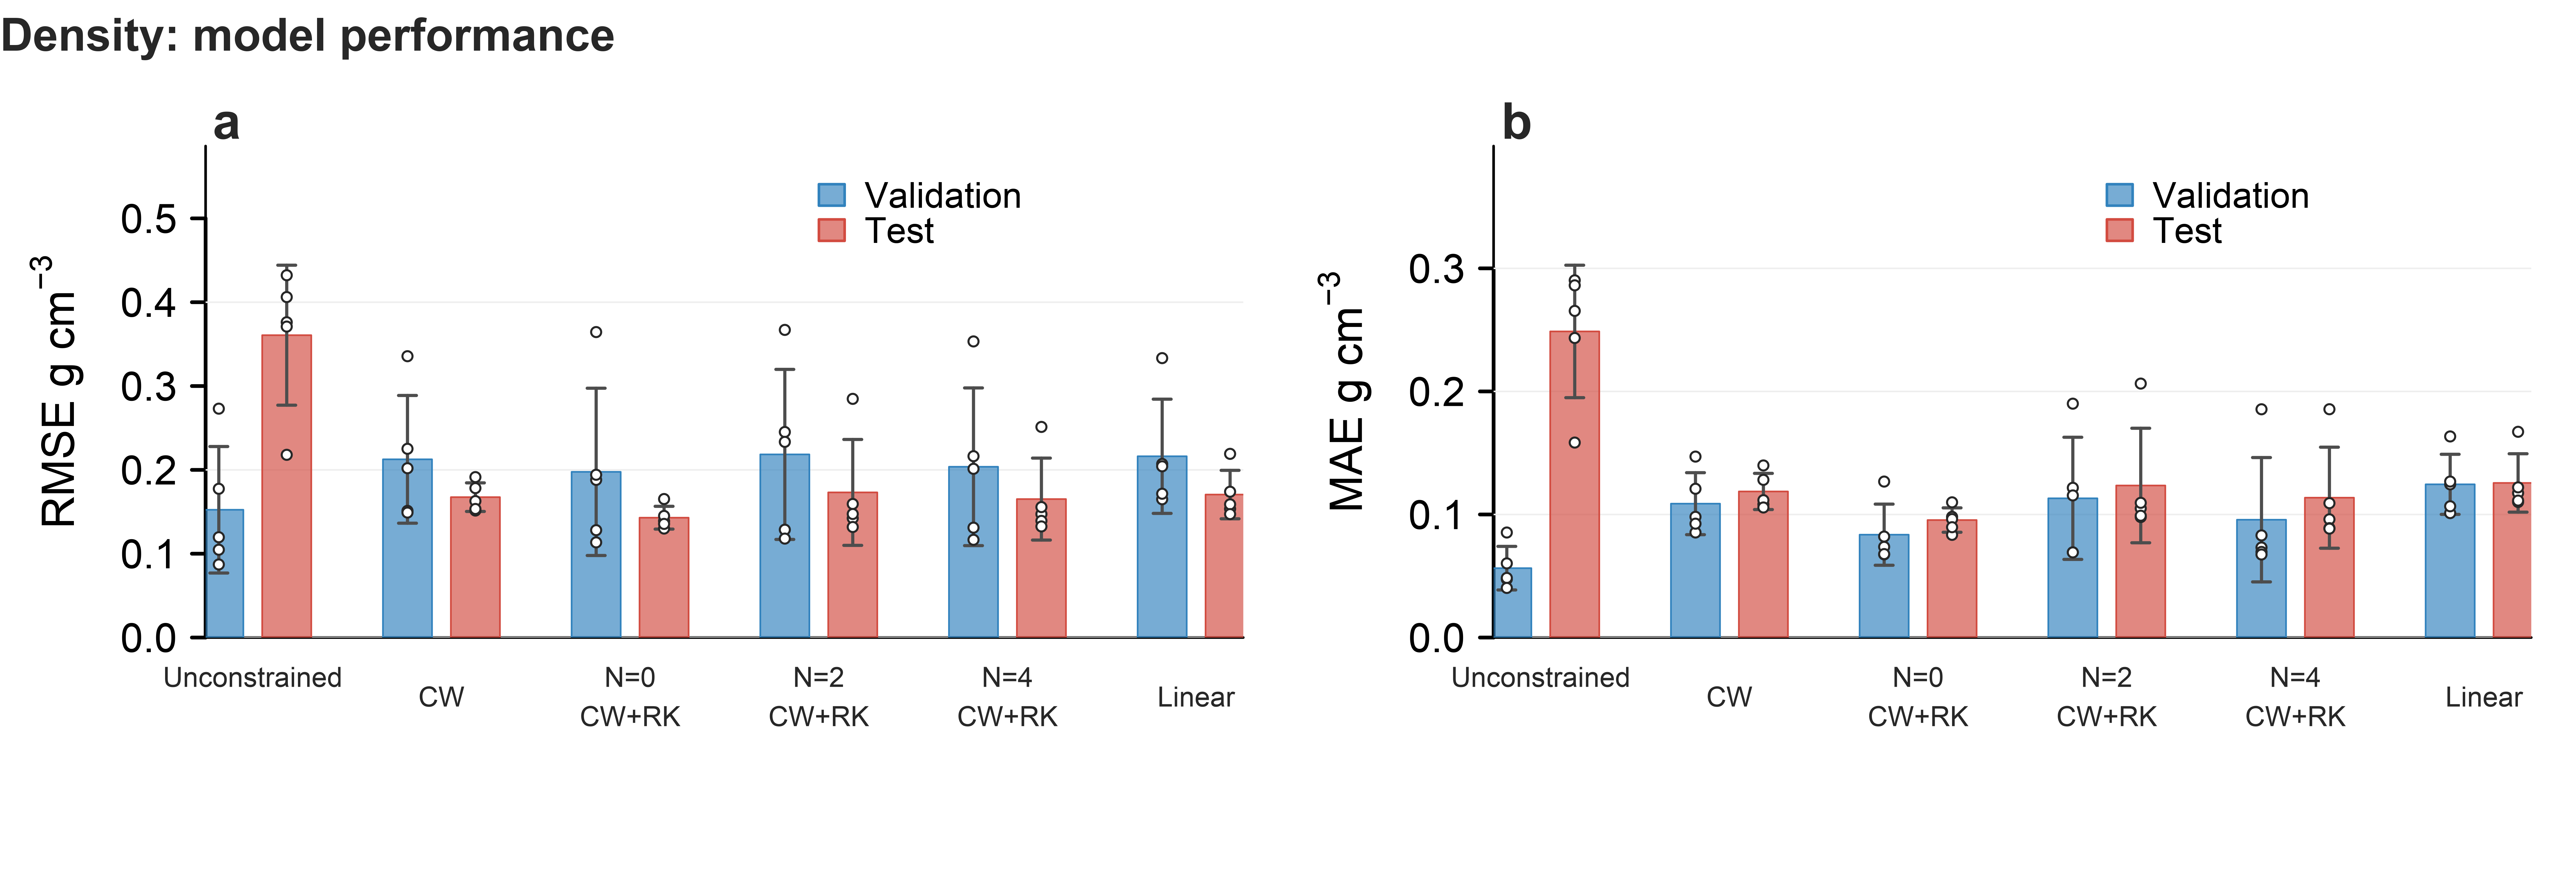
\includegraphics[width=\linewidth,height=0.68\textheight,keepaspectratio]{figures-SI/density_rmse_mae_by_n.png}
\captionof{figure}{不同模型变体和 RK 阶数下的密度 RMSE 与 MAE 比较。}
\label{fig:si-density-rmse-mae}
\end{minipage}
\end{center}

\begin{center}
\begin{minipage}{\linewidth}
\centering
\makebox[\linewidth][c]{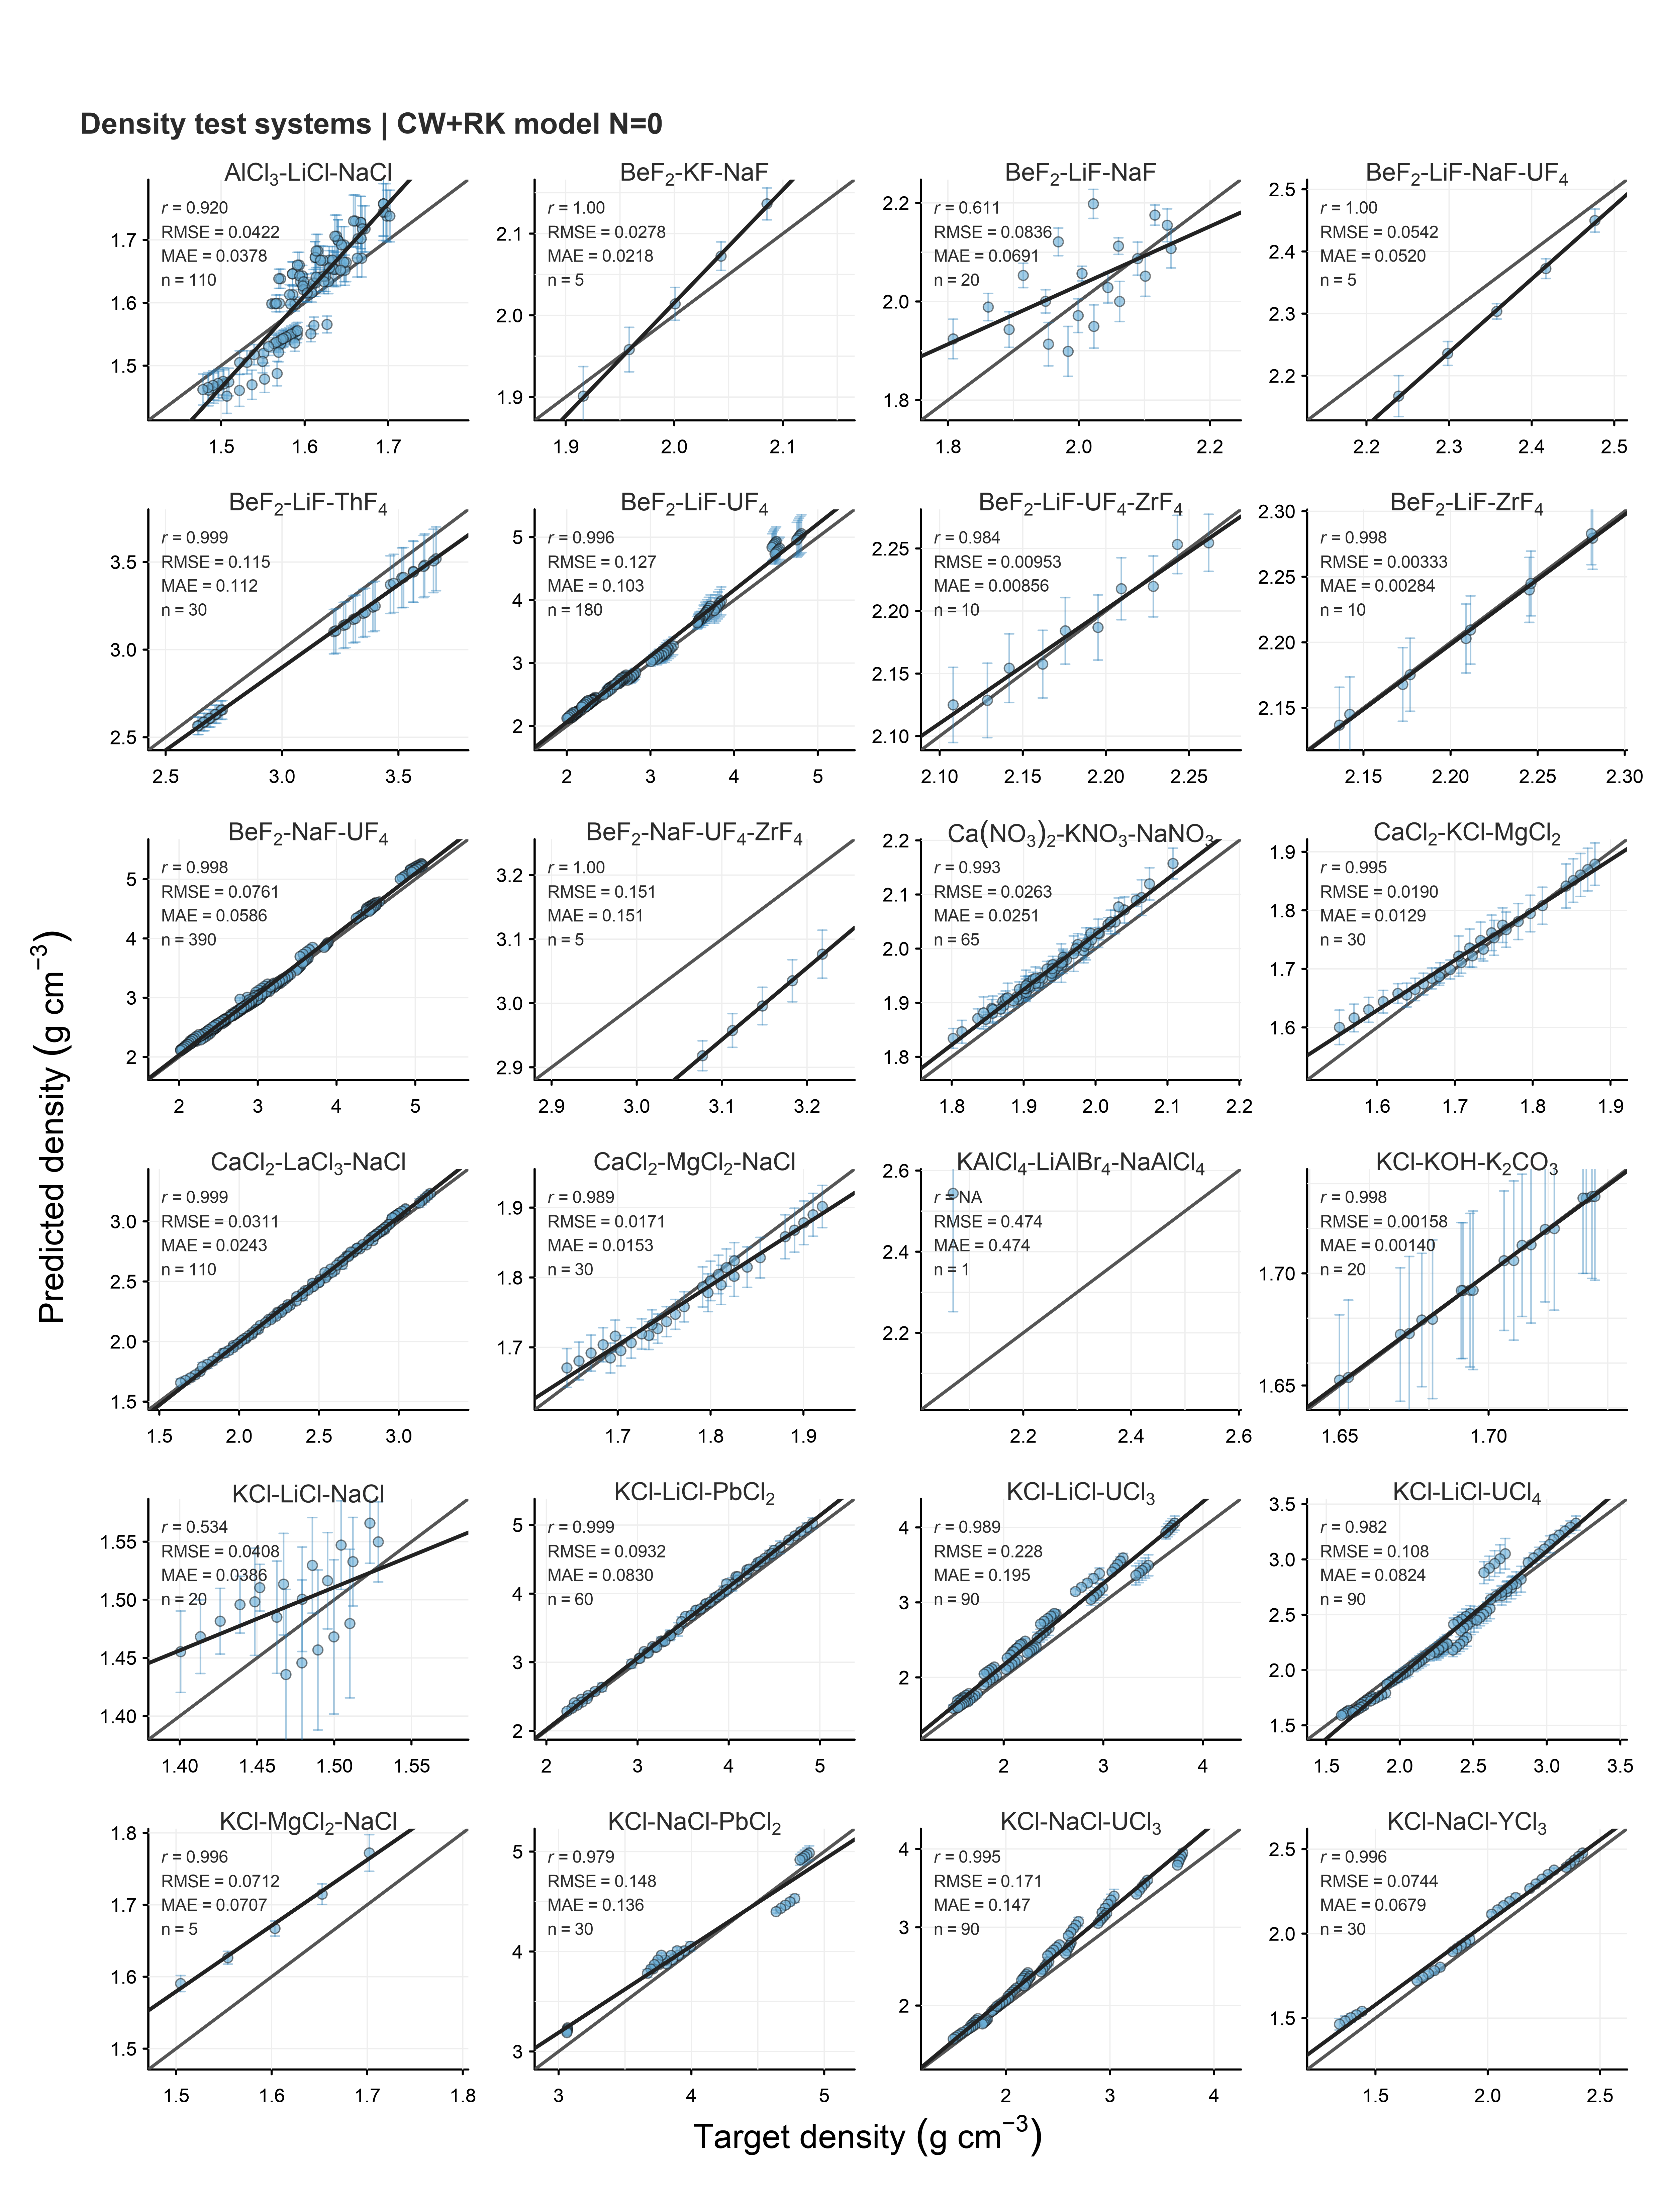
\includegraphics[width=\linewidth]{figures-SI/density_test_system_correlation_grid_cw_rk_model_n_0_page_01.png}}
\end{minipage}
\end{center}

\begin{center}
\begin{minipage}{\linewidth}
\centering
\makebox[\linewidth][c]{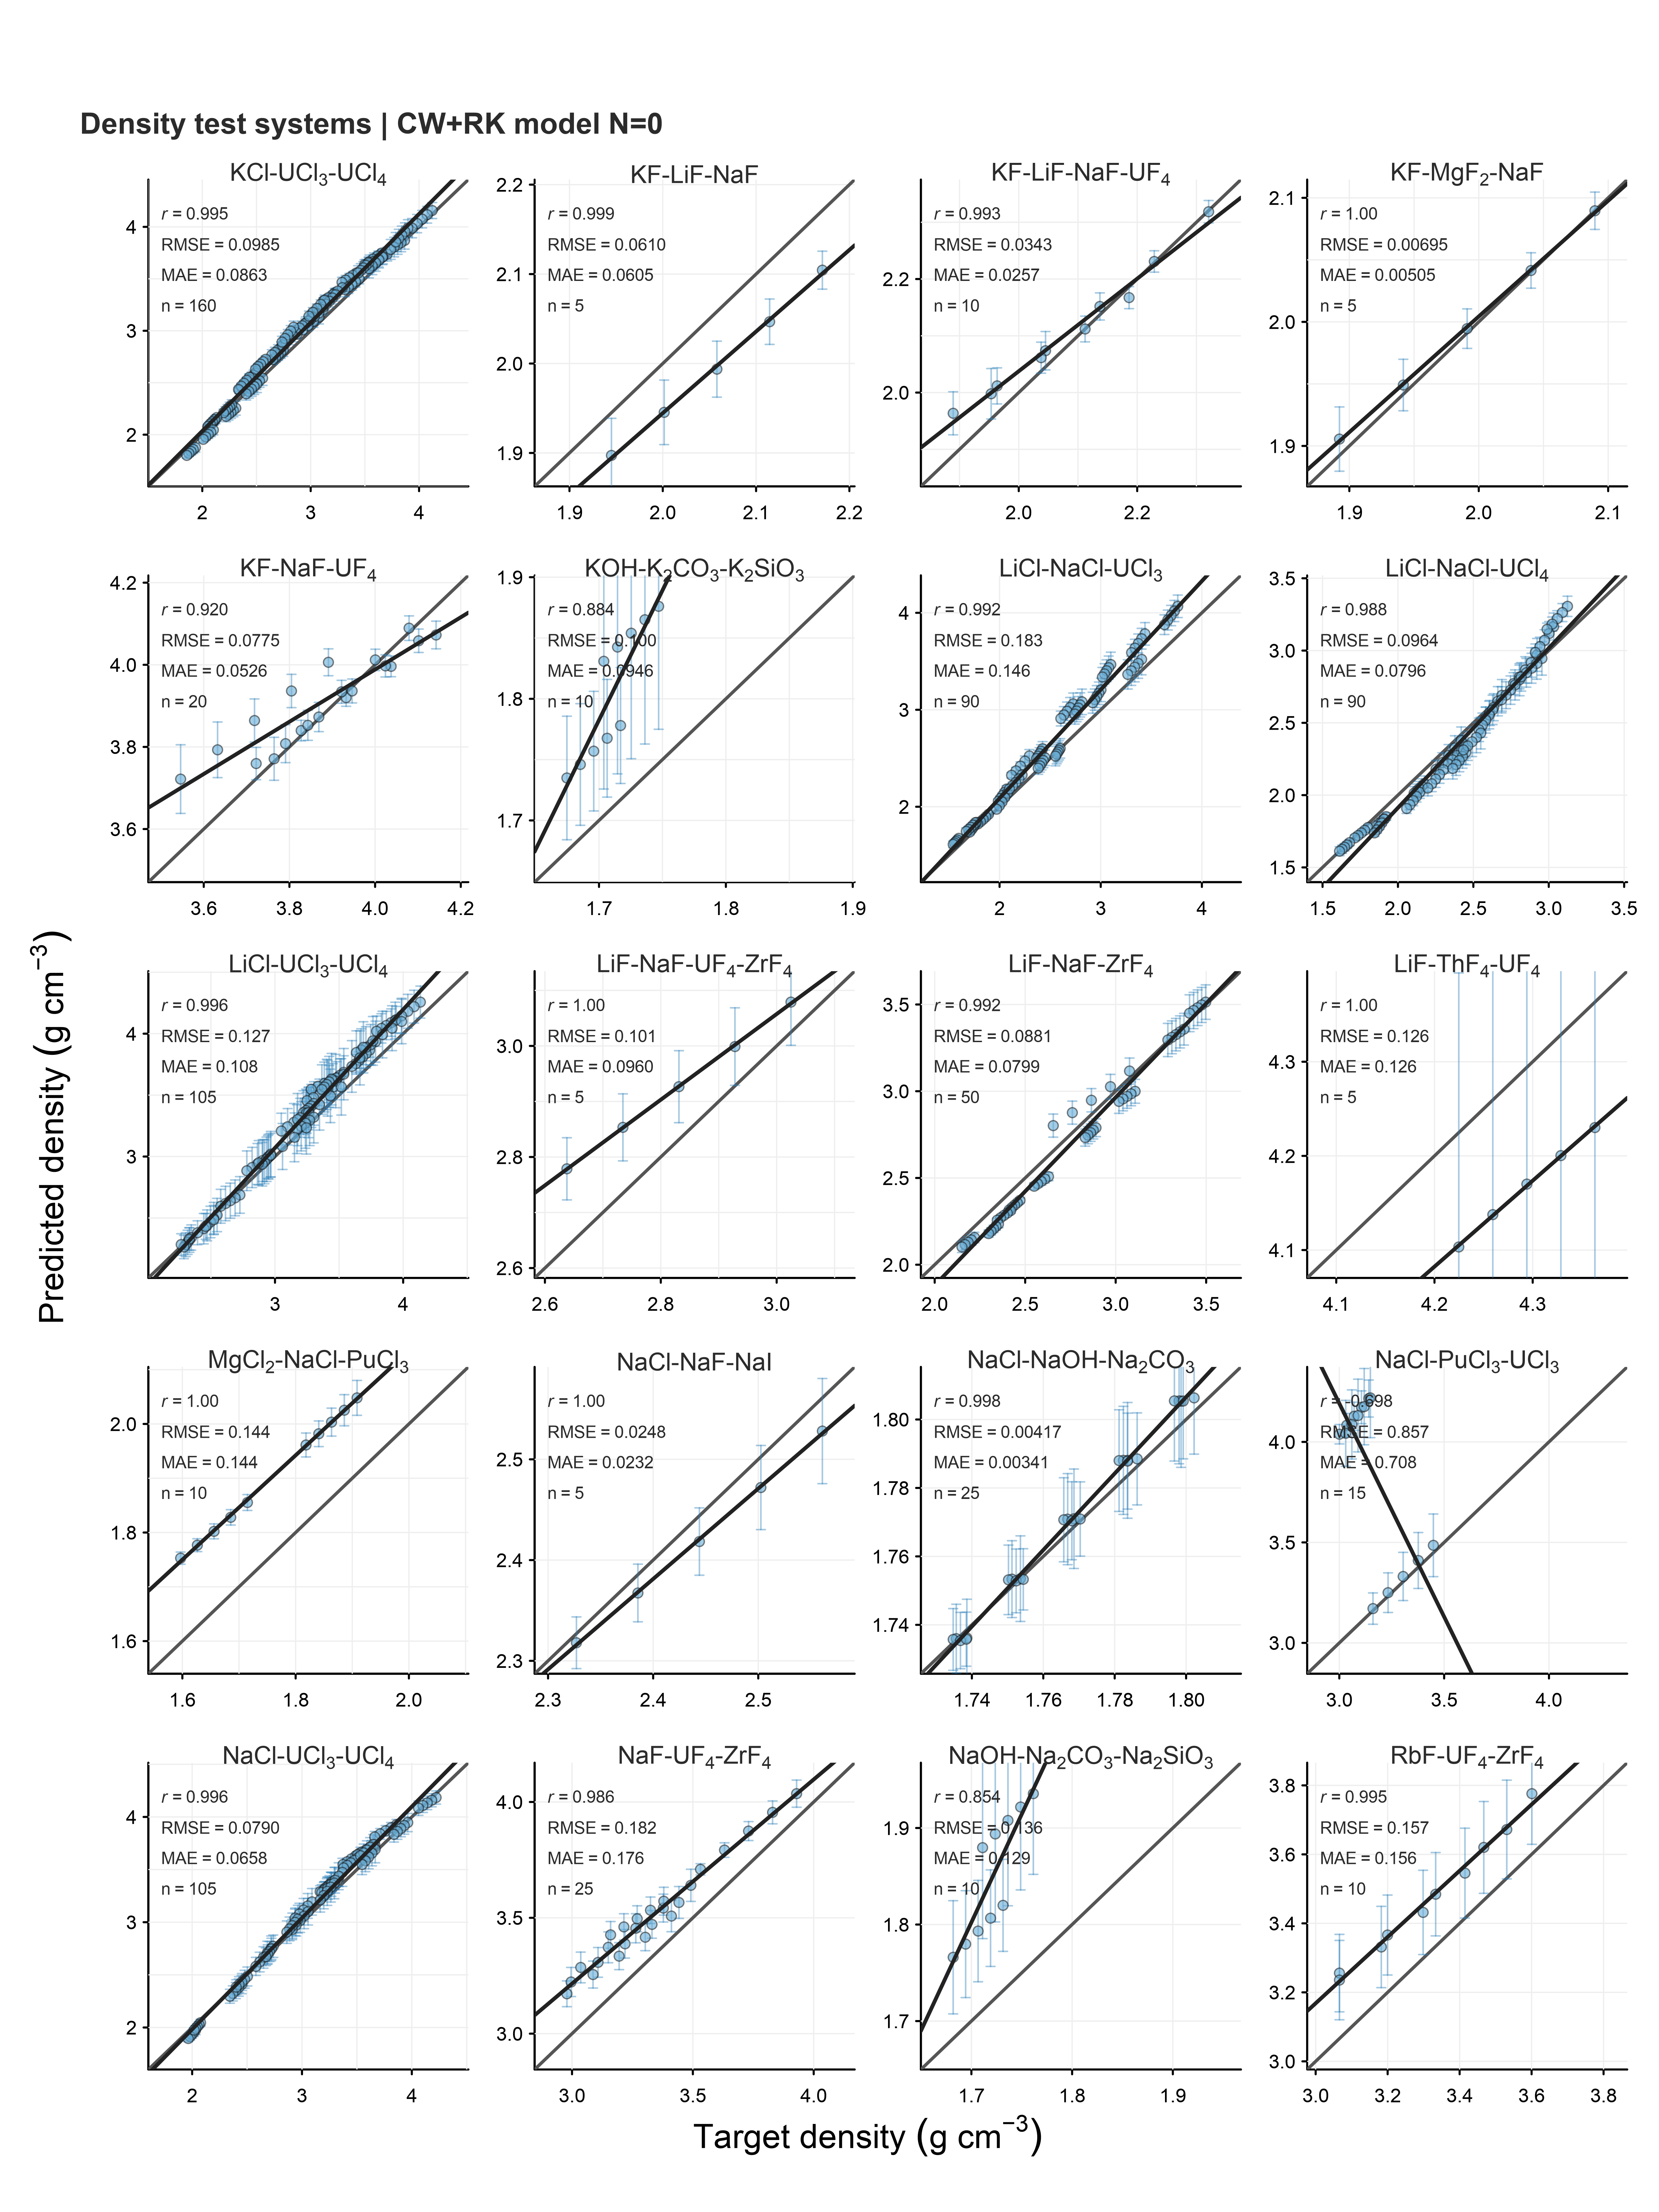
\includegraphics[width=\linewidth]{figures-SI/density_test_system_correlation_grid_cw_rk_model_n_0_page_02.png}}
\captionof{figure}{CW+RK 模型（\(N=0\)）在密度测试体系中的相关性网格图。}
\label{fig:si-density-test-correlation}
\end{minipage}
\end{center}

三元测试体系中最大的密度误差主要集中在低阶覆盖不完整的锕系氯化物和氟化物体系。最明显的离群体系是 NaCl--PuCl\(_3\)--UCl\(_3\)，其 MAE 为 0.708，最大绝对误差为 1.075；模型对该体系存在系统性高估。这一现象与纯 PuCl\(_3\) 记录缺失以及 PuCl\(_3\)--UCl\(_3\) 二元覆盖缺失一致，最大偏差出现在低 NaCl、高 Pu/U 氯化物组成区域。KAlCl\(_4\)--LiAlBr\(_4\)--NaAlCl\(_4\) 也表现出较大误差（MAE = 0.474），因为三个伪组分及其所有对应二元子体系都不在低阶训练池中，该案例接近完全外推。其他高误差三元氟化物体系，例如 NaF--UF\(_4\)--ZrF\(_4\) 和 RbF--UF\(_4\)--ZrF\(_4\)，主要受到 UF\(_4\)--ZrF\(_4\) 二元覆盖缺失以及含 RbF 二元数据稀疏的影响。此外，即使 KCl/LiCl/NaCl--UCl\(_3\) 家族的一元和二元子体系覆盖较充分，预测仍存在偏差，说明三元锕系氯化物的非理想行为不能仅由现有二元 RK 项和组成加权项充分推断。

对于四元密度体系，误差整体较为温和。误差最大的体系是 BeF\(_2\)--NaF--UF\(_4\)--ZrF\(_4\)，MAE 为 0.151，其中 BeF\(_2\)--ZrF\(_4\) 和 UF\(_4\)--ZrF\(_4\) 二元覆盖缺失。LiF--NaF--UF\(_4\)--ZrF\(_4\) 的 MAE 为 0.096，主要受 UF\(_4\)--ZrF\(_4\) 子体系缺失限制。

\subsection*{3.2 表面张力}\label{surface-tension-figures}

\begin{center}
\begin{minipage}{\linewidth}
\centering
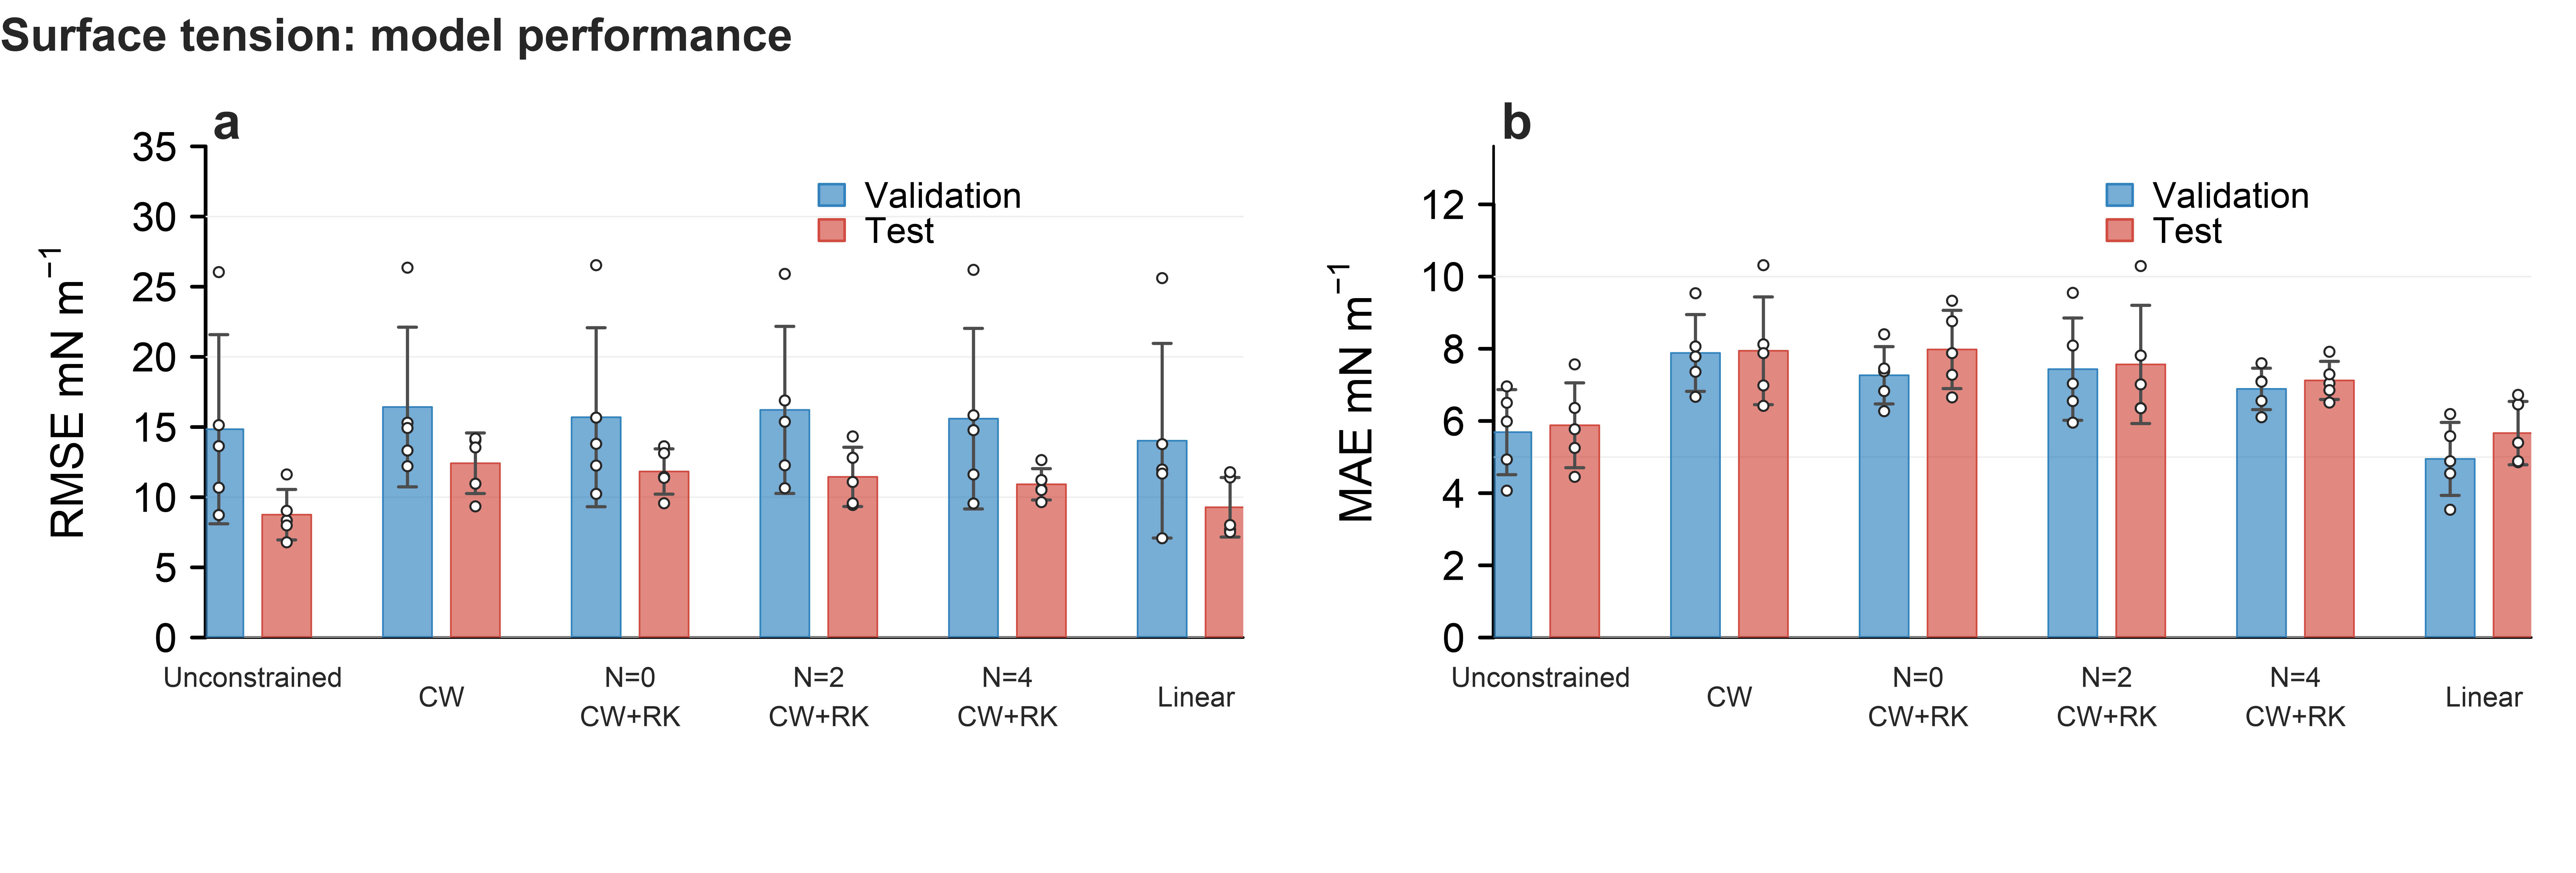
\includegraphics[width=\linewidth,height=0.68\textheight,keepaspectratio]{figures-SI/surface_tension_rmse_mae_by_n.png}
\captionof{figure}{不同模型变体和 RK 阶数下的表面张力 RMSE 与 MAE 比较。}
\label{fig:si-surface-tension-rmse-mae}
\end{minipage}
\end{center}

\begin{center}
\begin{minipage}{\linewidth}
\centering
\makebox[\linewidth][c]{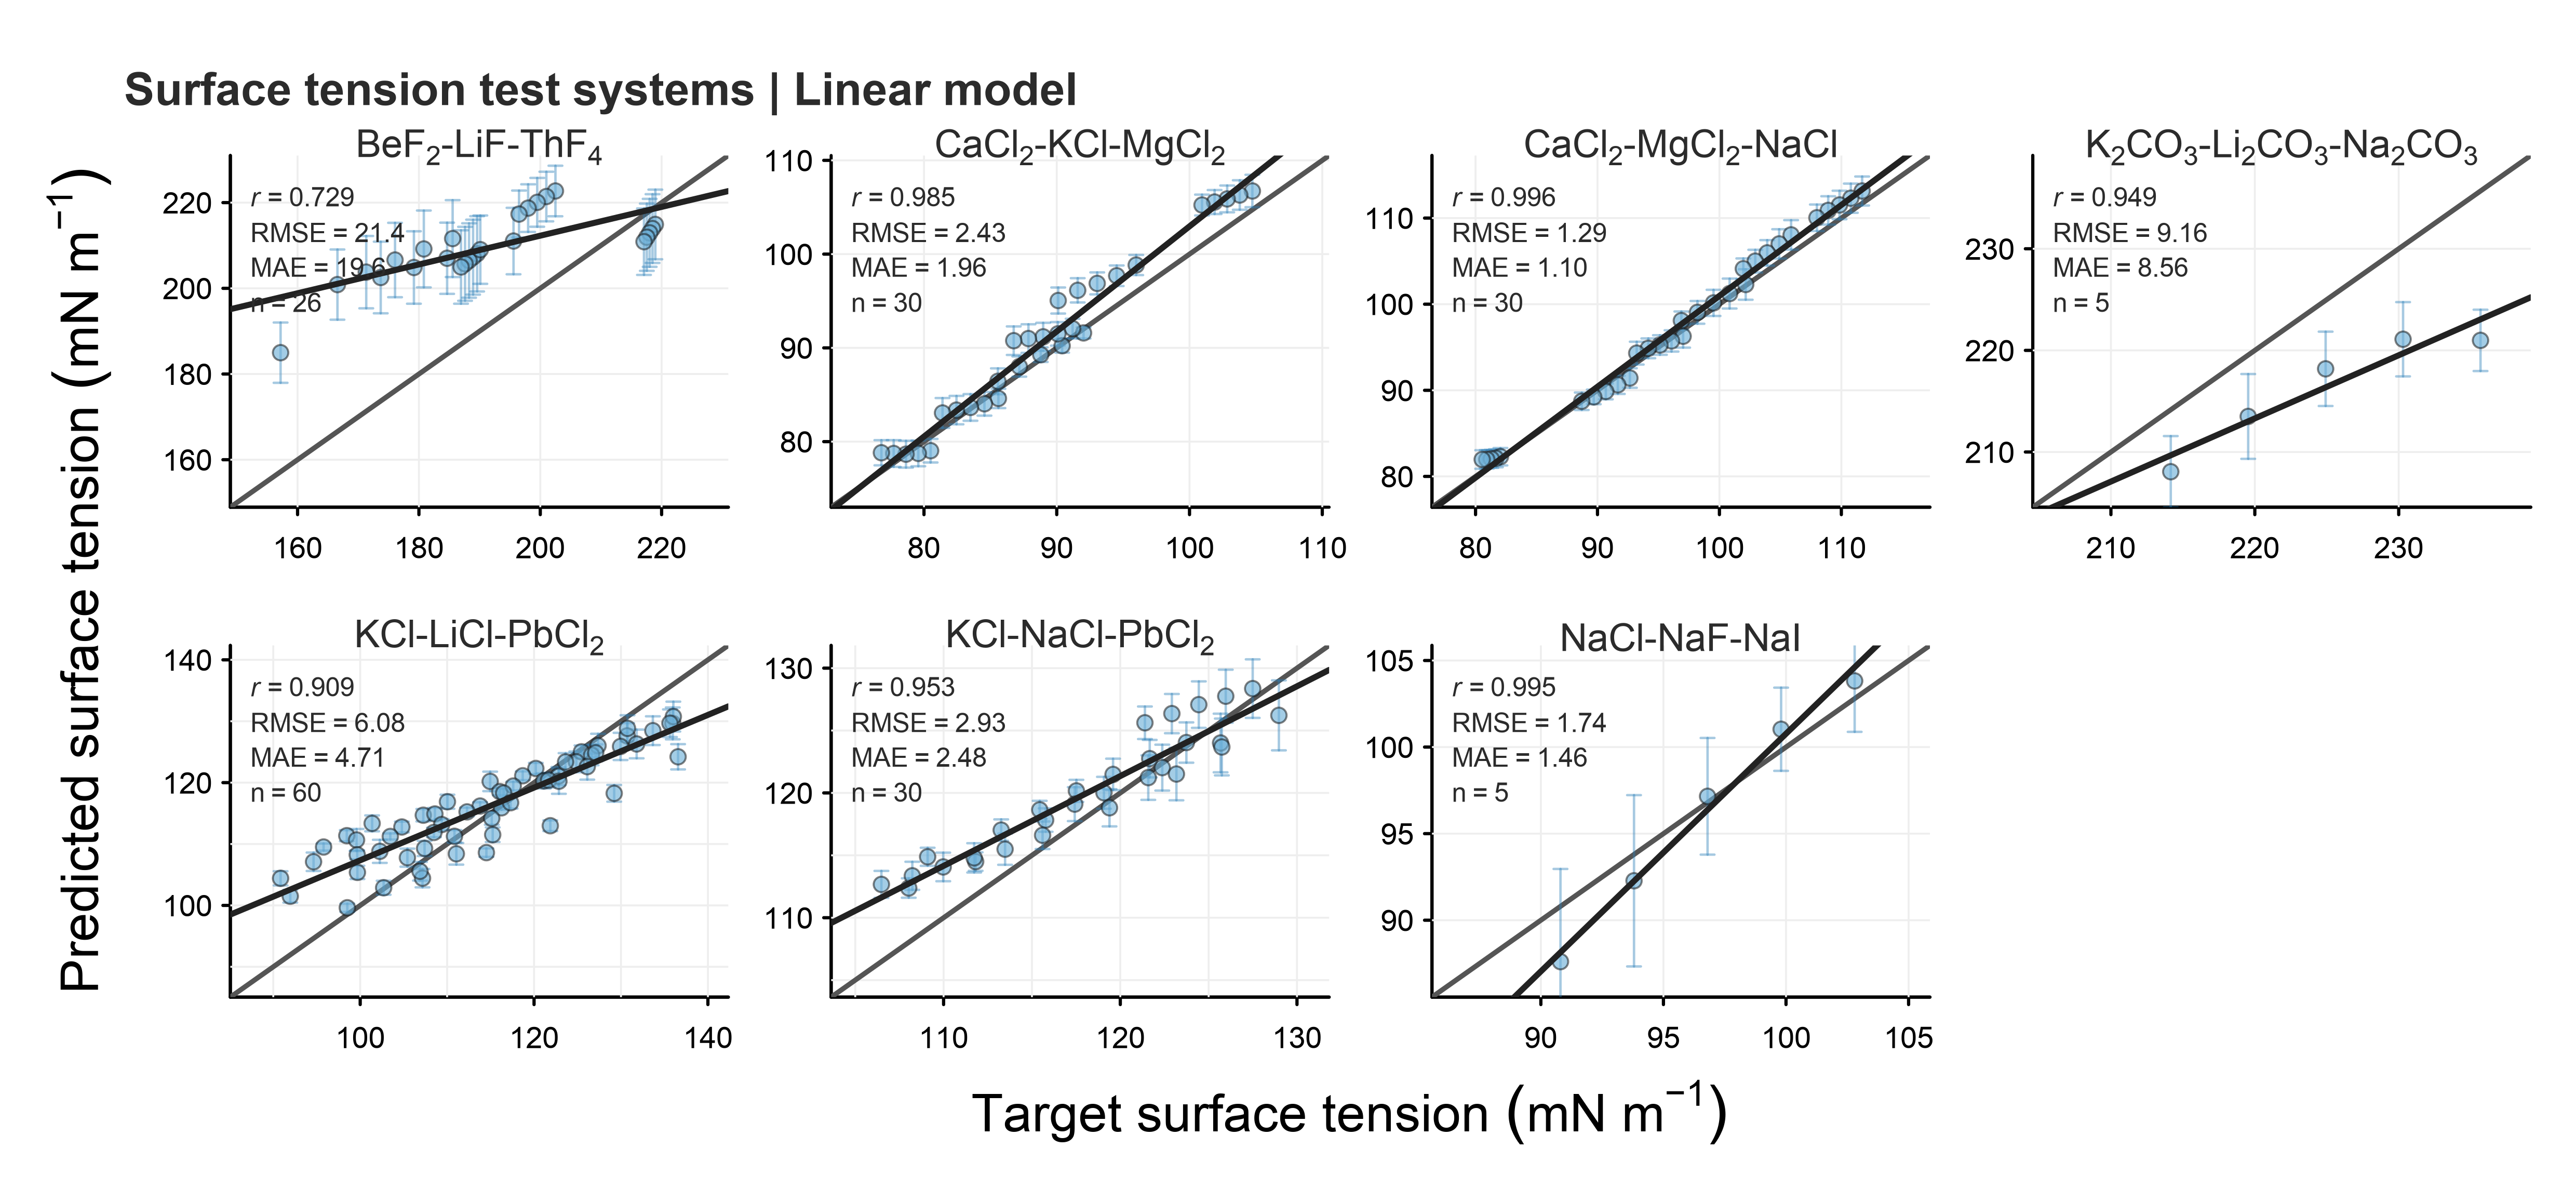
\includegraphics[width=\linewidth]{figures-SI/surface_tension_test_system_correlation_grid_linear_model_page_01.png}}
\captionof{figure}{线性约束模型在表面张力测试体系中的相关性网格图。}
\label{fig:si-surface-tension-test-correlation}
\end{minipage}
\end{center}

对于表面张力，最大的三元误差出现在 BeF\(_2\)--LiF--ThF\(_4\)，其 MAE 为 19.623 mN m\(^{-1}\)，最大绝对误差为 34.297 mN m\(^{-1}\)。模型对该体系存在系统性高估，尤其是在目标值较低的记录中更为明显。这一行为与低阶覆盖不完整一致：低阶数据池中没有纯 BeF\(_2\) 表面张力记录，同时也缺少 BeF\(_2\)--ThF\(_4\) 二元子体系。K\(_2\)CO\(_3\)--Li\(_2\)CO\(_3\)--Na\(_2\)CO\(_3\) 的一元和二元覆盖完整，但仍表现出较大的 MAE（8.556 mN m\(^{-1}\)），主要原因是模型低估了该三元碳酸盐记录的高表面张力端。这表明仅依靠低阶数据，线性约束模型未能捕捉到该三元体系的组成或温度非线性。

KCl--LiCl--PbCl\(_2\) 和 KCl--NaCl--PbCl\(_2\) 体系的偏差较小但仍然可见，MAE 分别为 4.706 和 2.475 mN m\(^{-1}\)。它们的一元和二元子体系覆盖相对充分，因此这些误差较少由覆盖缺失导致，更可能反映富 PbCl\(_2\) 低温组成中的局部三元偏差。该测试集中没有四元表面张力体系。

\subsection*{3.3 黏度}\label{viscosity-figures}

\begin{center}
\begin{minipage}{\linewidth}
\centering
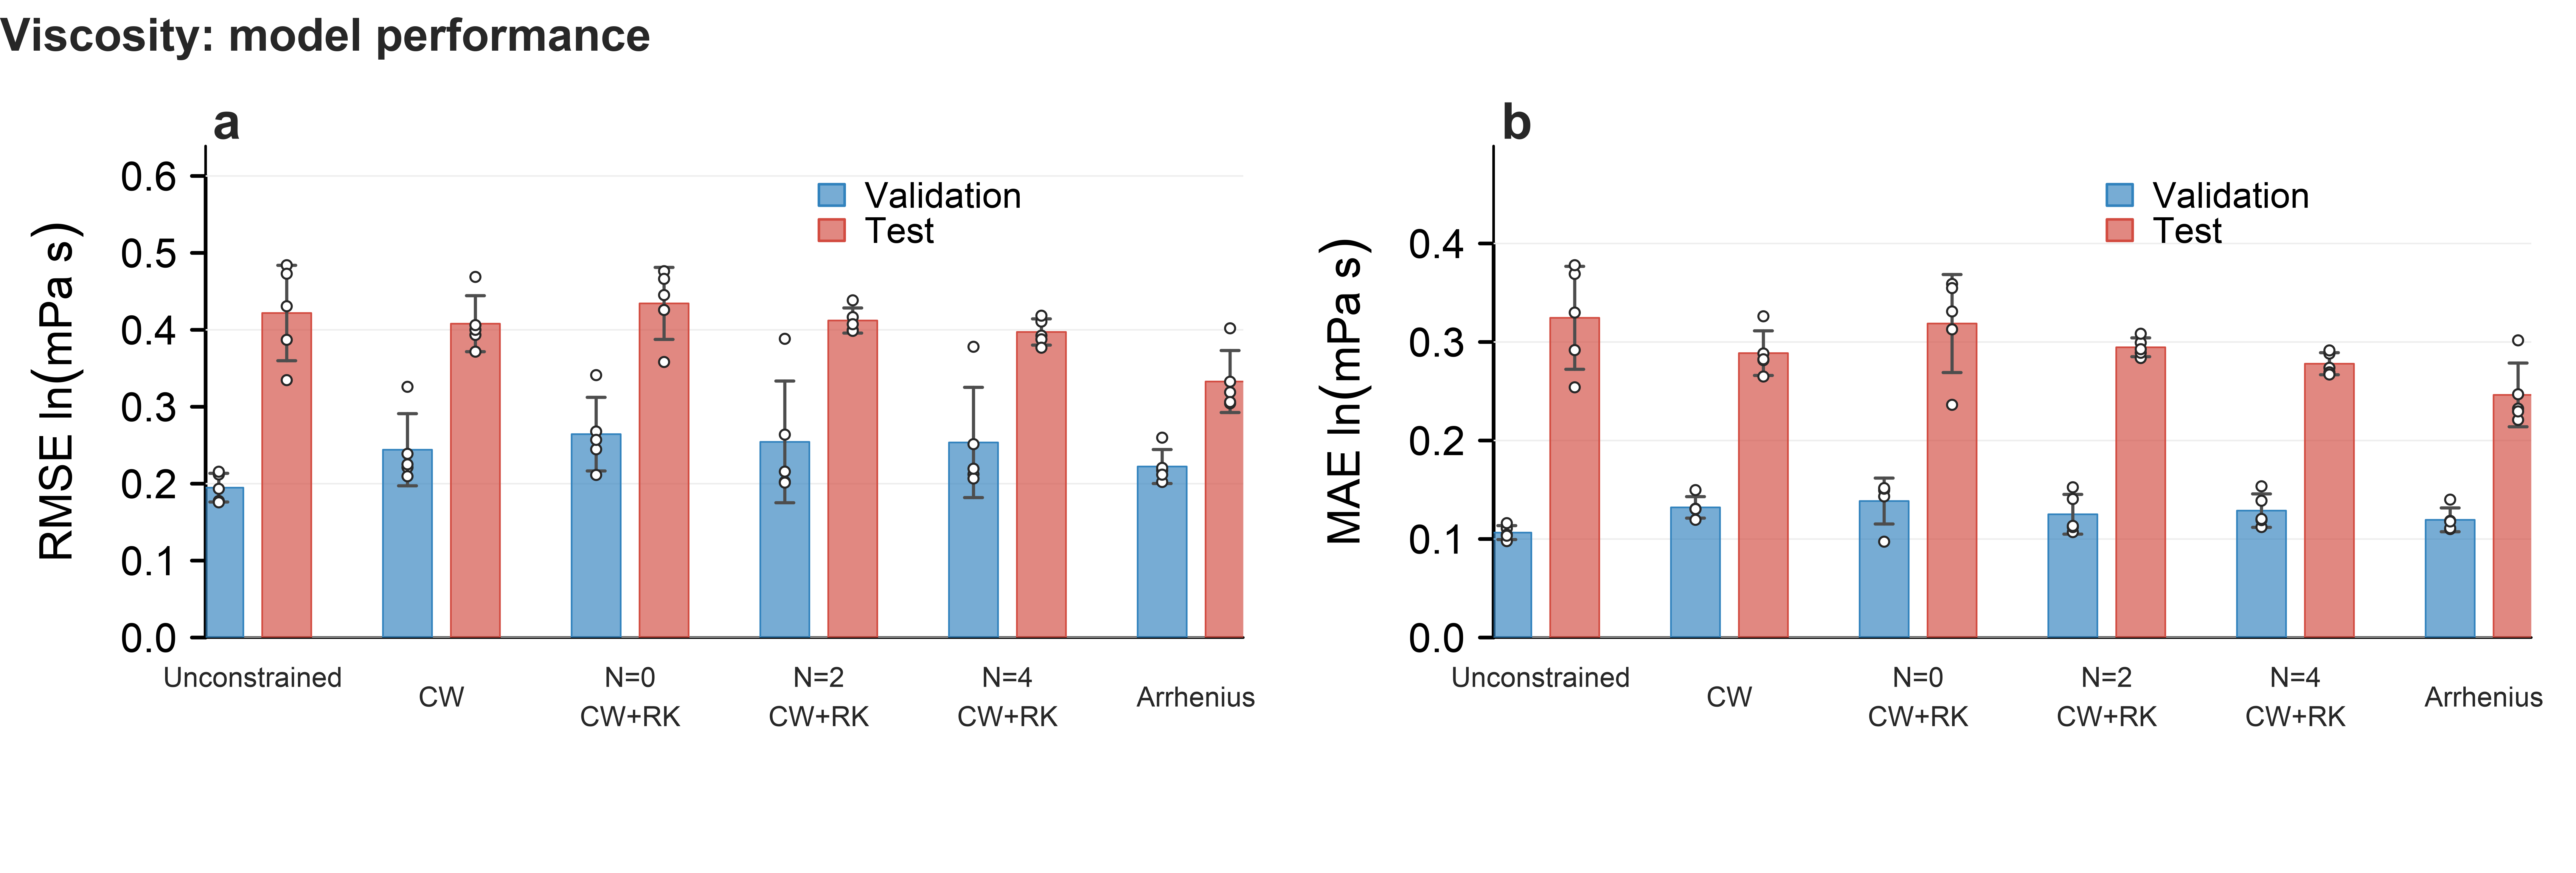
\includegraphics[width=\linewidth,height=0.68\textheight,keepaspectratio]{figures-SI/viscosity_rmse_mae_by_n.png}
\captionof{figure}{不同模型变体和 RK 阶数下的黏度 RMSE 与 MAE 比较。}
\label{fig:si-viscosity-rmse-mae}
\end{minipage}
\end{center}

\begin{center}
\begin{minipage}{\linewidth}
\centering
\makebox[\linewidth][c]{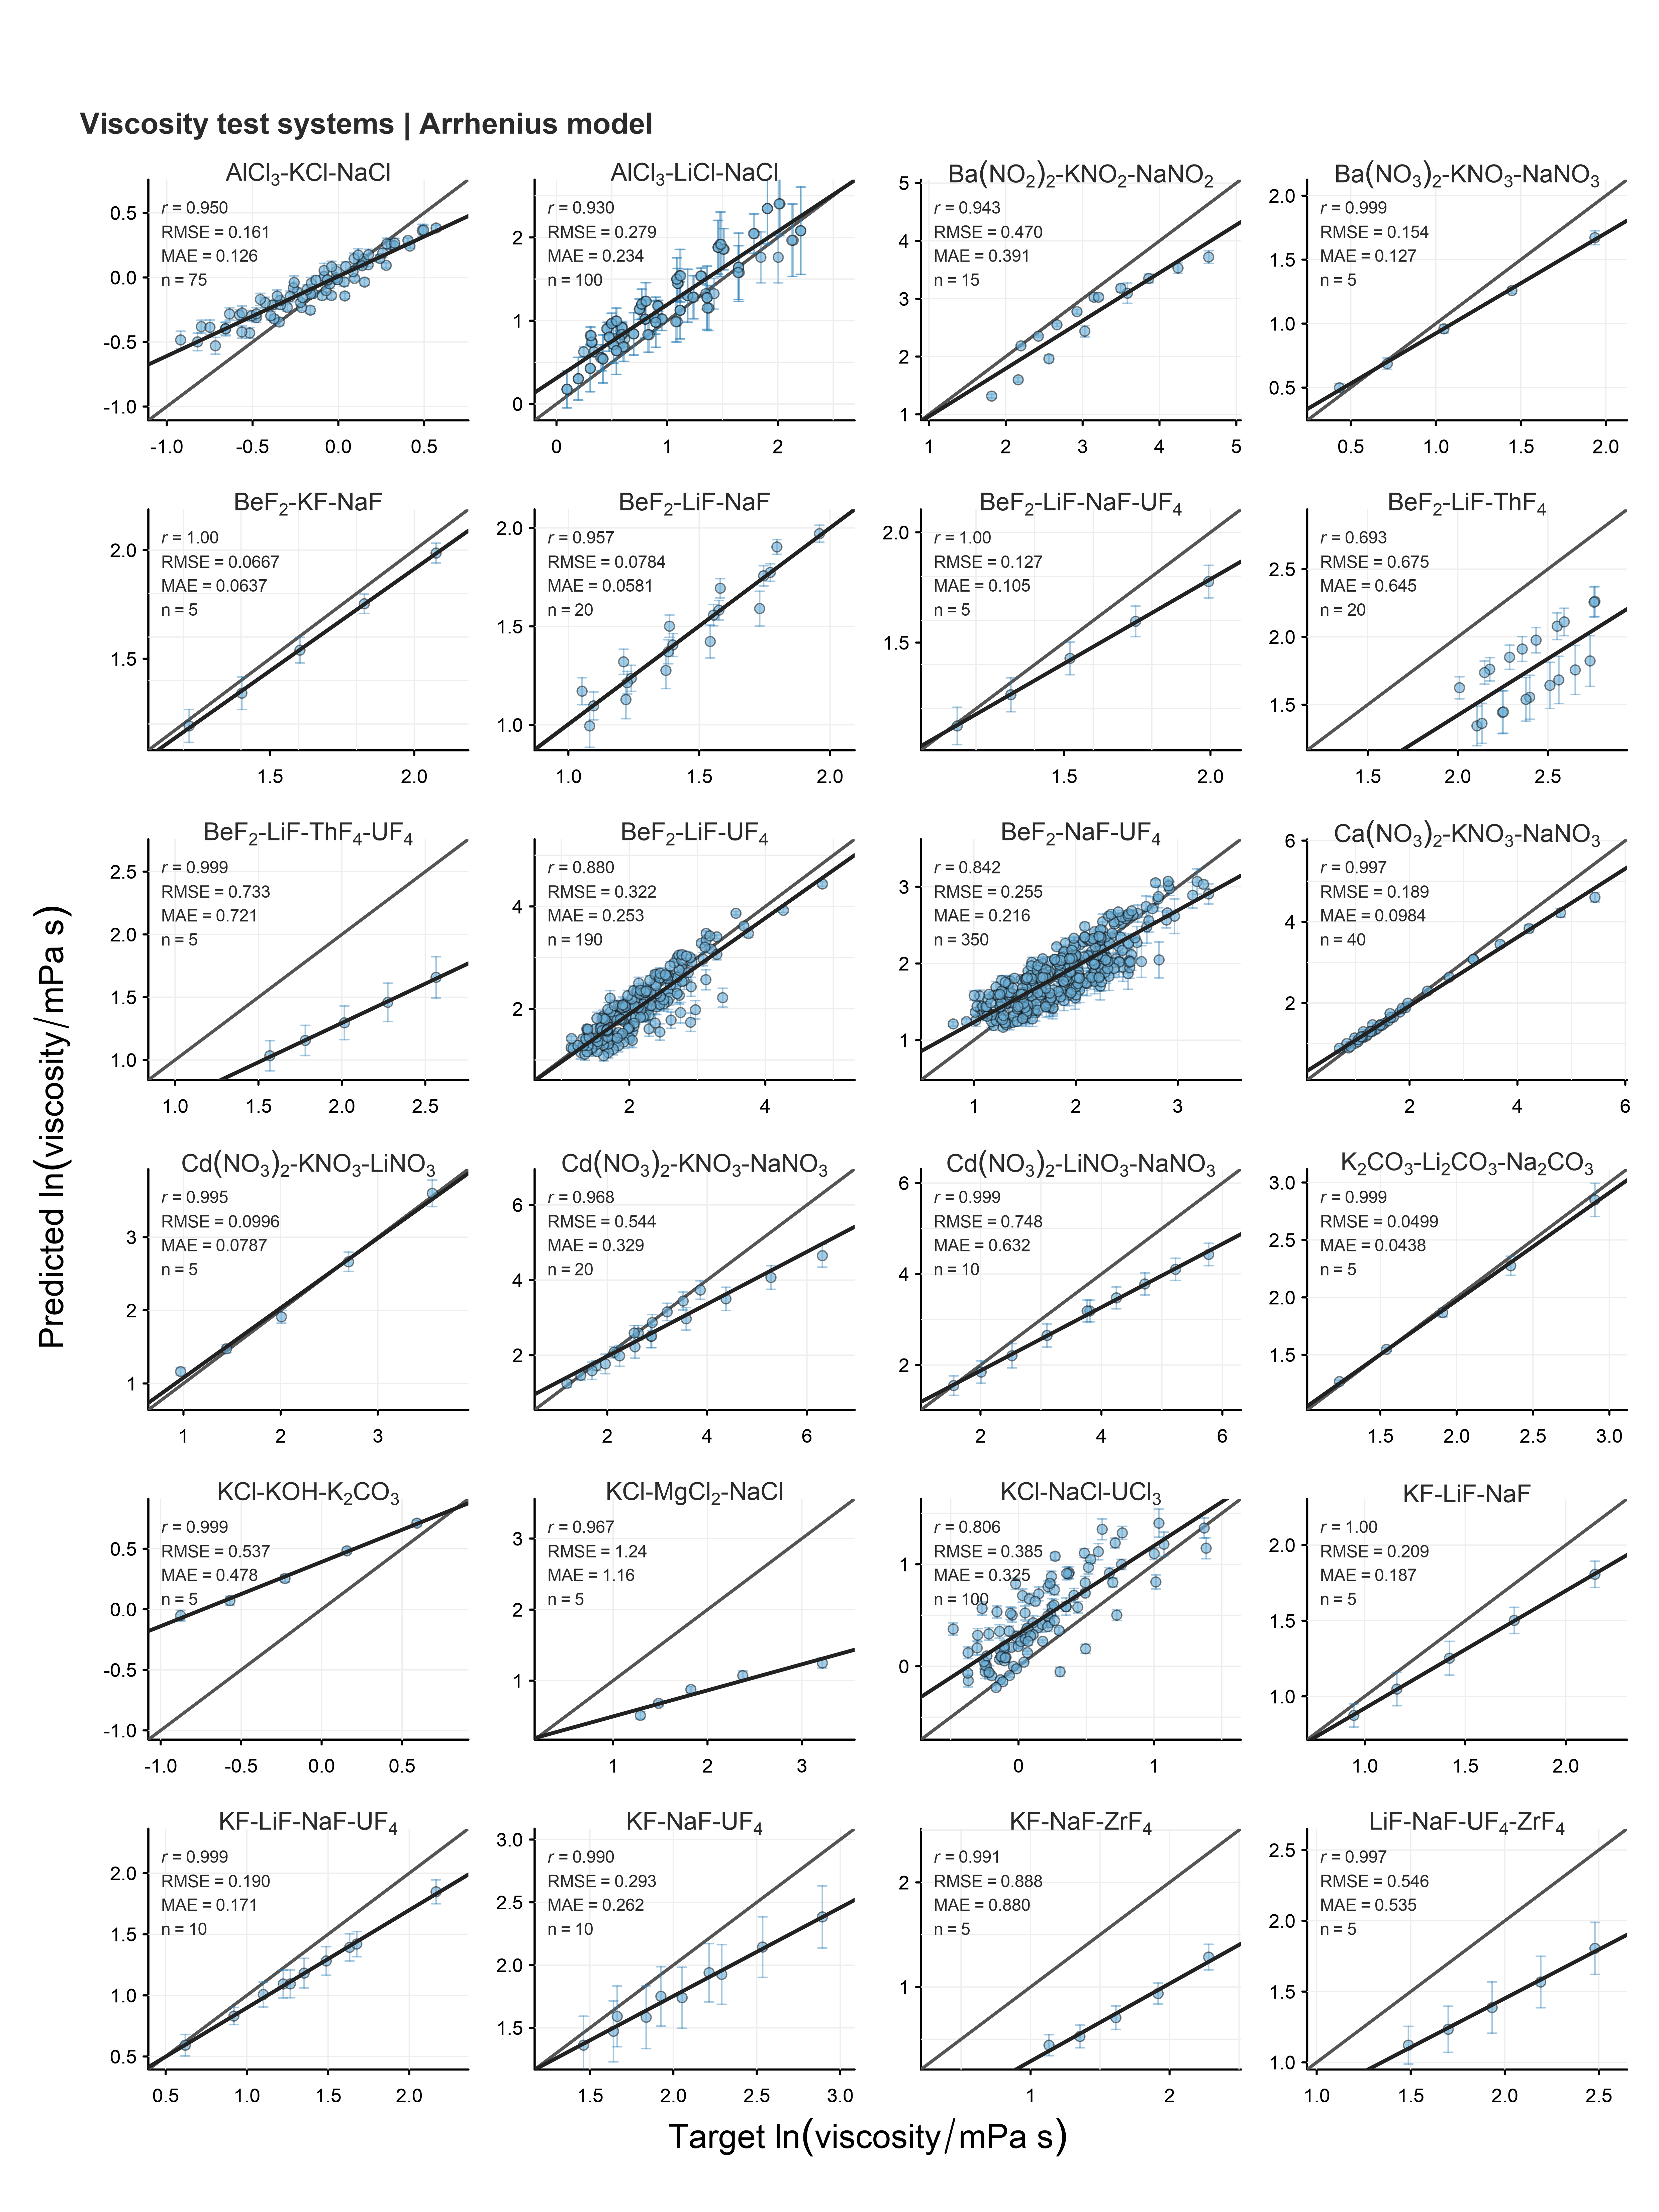
\includegraphics[width=\linewidth]{figures-SI/viscosity_test_system_correlation_grid_arrhenius_model_page_01.png}}
\end{minipage}
\end{center}

\begin{center}
\begin{minipage}{\linewidth}
\centering
\makebox[\linewidth][c]{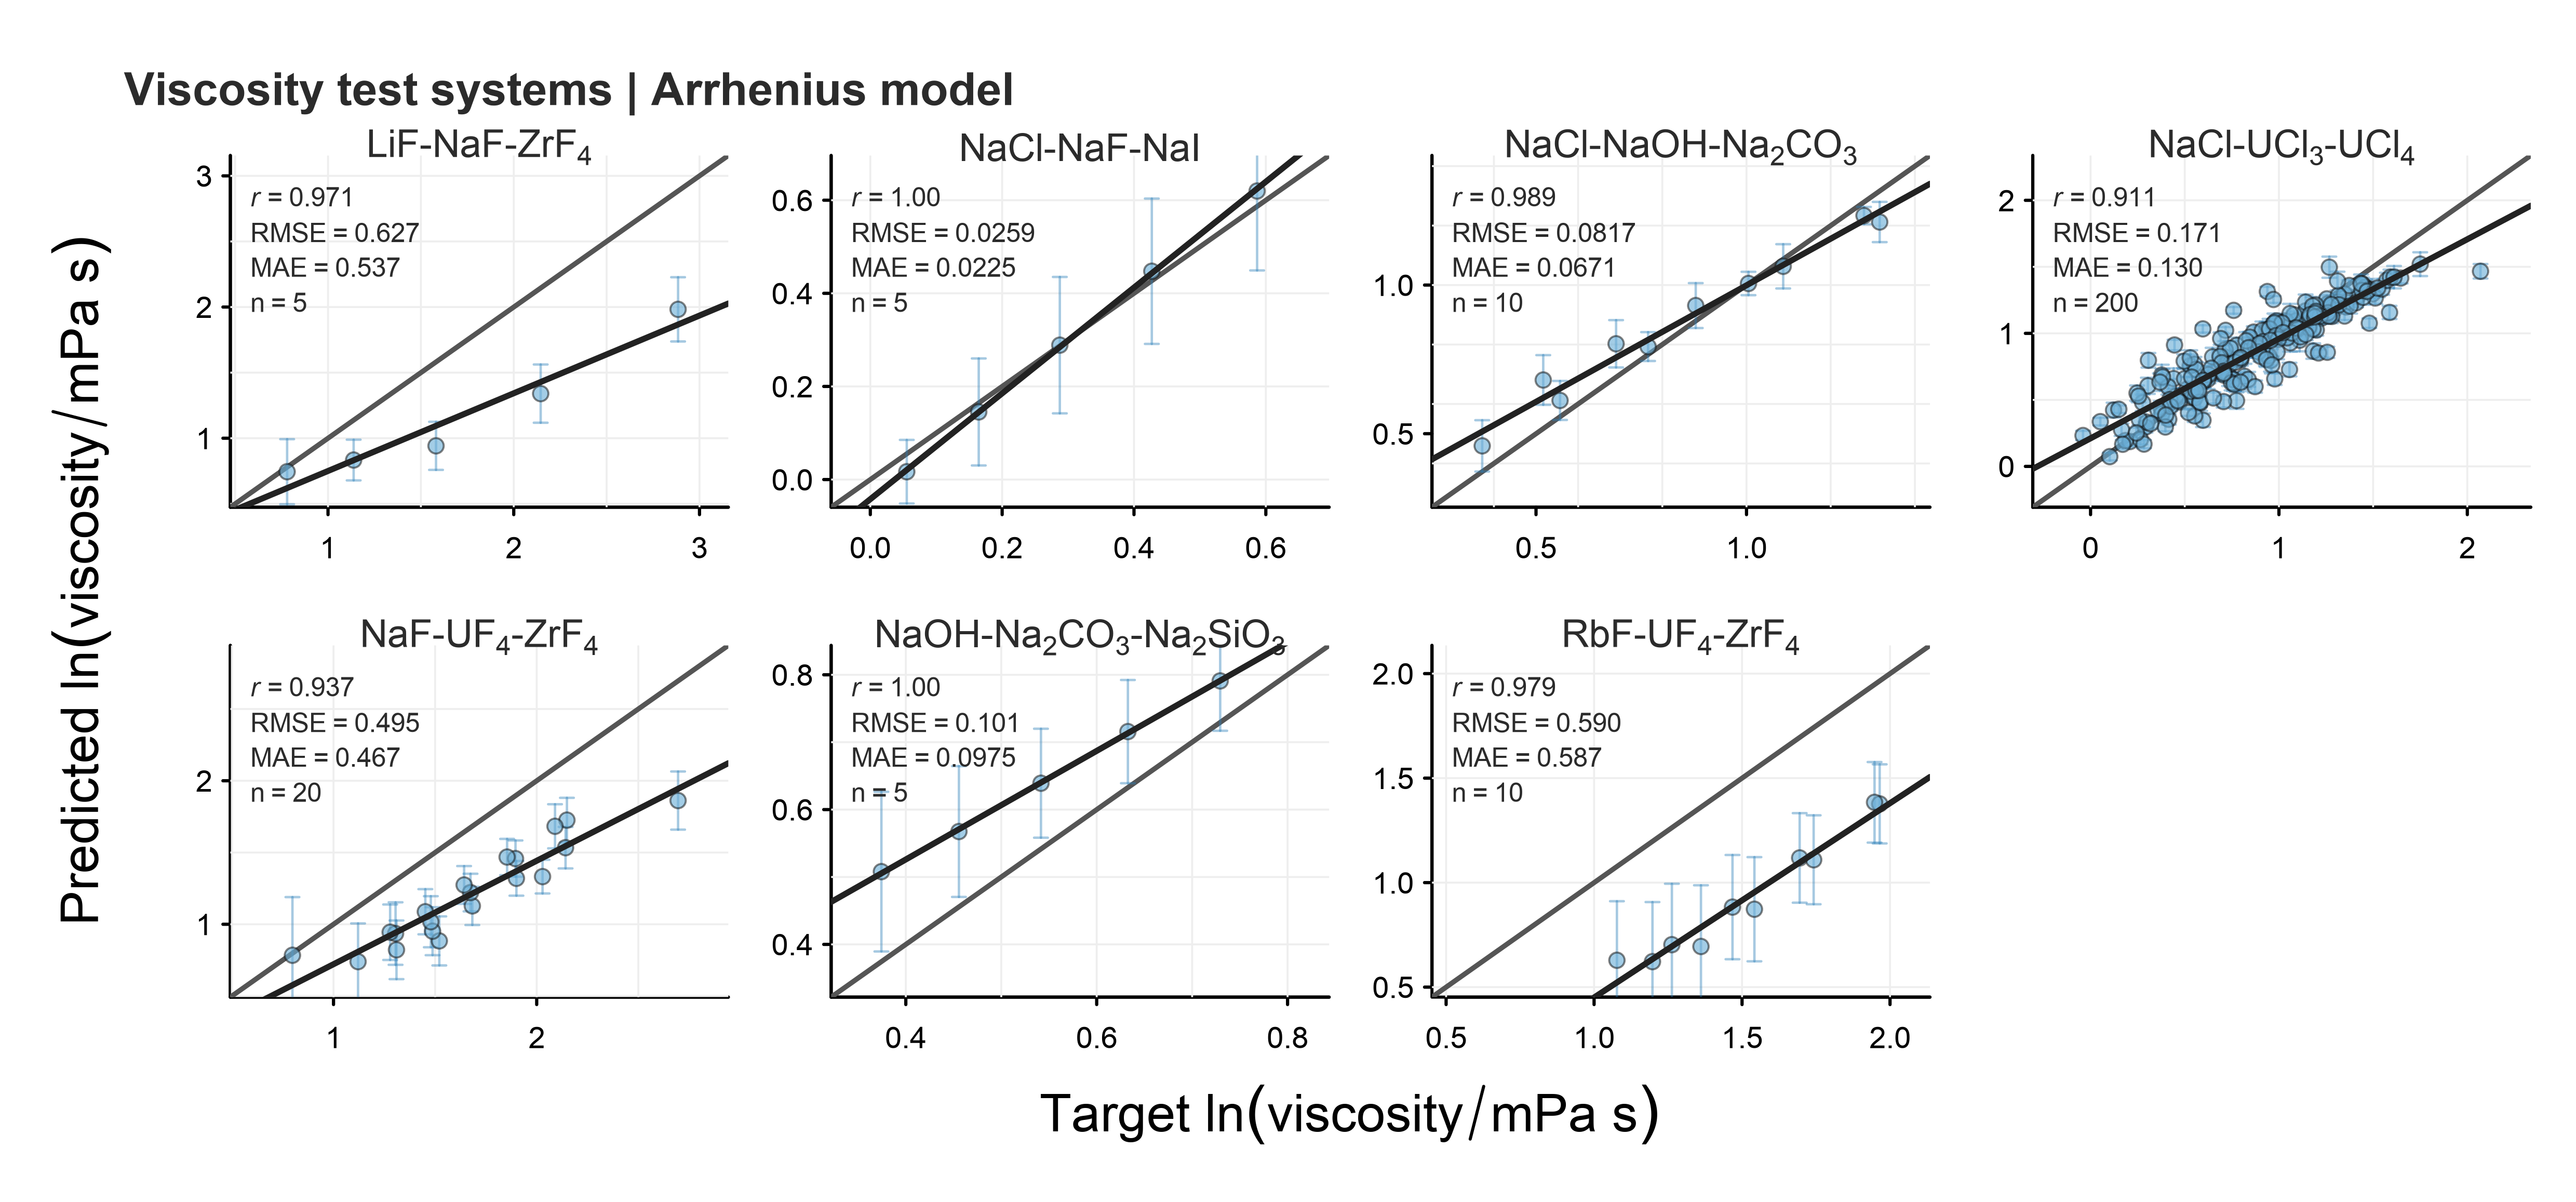
\includegraphics[width=\linewidth]{figures-SI/viscosity_test_system_correlation_grid_arrhenius_model_page_02.png}}
\captionof{figure}{Arrhenius 约束模型在黏度测试体系中的相关性网格图。}
\label{fig:si-viscosity-test-correlation}
\end{minipage}
\end{center}

对于黏度，最大的三元误差主要对应 Arrhenius 约束模型低估的低温高黏度区域。KCl--MgCl\(_2\)--NaCl 的三元误差最大，对数空间 MAE 为 1.160，最大绝对误差为 1.968；尽管其一元和二元子体系均有覆盖，仍出现较大偏差。最大偏差出现在目标对数黏度最高的点，说明低阶 Arrhenius 趋势未能充分再现该三元组成中黏度随温度降低而急剧升高的行为。KF--NaF--ZrF\(_4\) 和 LiF--NaF--ZrF\(_4\) 也表现出较大的对数空间 MAE，分别为 0.880 和 0.537；这些案例受到纯 ZrF\(_4\) 黏度覆盖缺失，以及含 ZrF\(_4\) 二元子体系稀疏或缺失的影响。

其他若干高误差三元体系同时具有低阶覆盖缺失和强非理想高价组分。BeF\(_2\)--LiF--ThF\(_4\) 的对数空间 MAE 为 0.645，缺少纯 ThF\(_4\)、BeF\(_2\)--ThF\(_4\) 和 LiF--ThF\(_4\) 黏度覆盖。RbF--UF\(_4\)--ZrF\(_4\) 和 NaF--UF\(_4\)--ZrF\(_4\) 也类似地受限于 ZrF\(_4\) 或 UF\(_4\)--ZrF\(_4\) 覆盖缺失。Cd(NO\(_3\))\(_2\)--LiNO\(_3\)--NaNO\(_3\) 和 Cd(NO\(_3\))\(_2\)--KNO\(_3\)--NaNO\(_3\) 同样被低估，这与纯 Cd(NO\(_3\))\(_2\) 以及含 Cd 二元记录缺失一致。对于四元黏度，BeF\(_2\)--LiF--ThF\(_4\)--UF\(_4\) 是误差最大的案例（对数空间 MAE = 0.721），其次是 LiF--NaF--UF\(_4\)--ZrF\(_4\)（对数空间 MAE = 0.535）；二者主要由 ThF\(_4\)、ZrF\(_4\) 或 UF\(_4\)--ZrF\(_4\) 低阶覆盖缺失主导。

\subsection*{3.4 电导率}\label{electrical-conductivity-figures}

\begin{center}
\begin{minipage}{\linewidth}
\centering
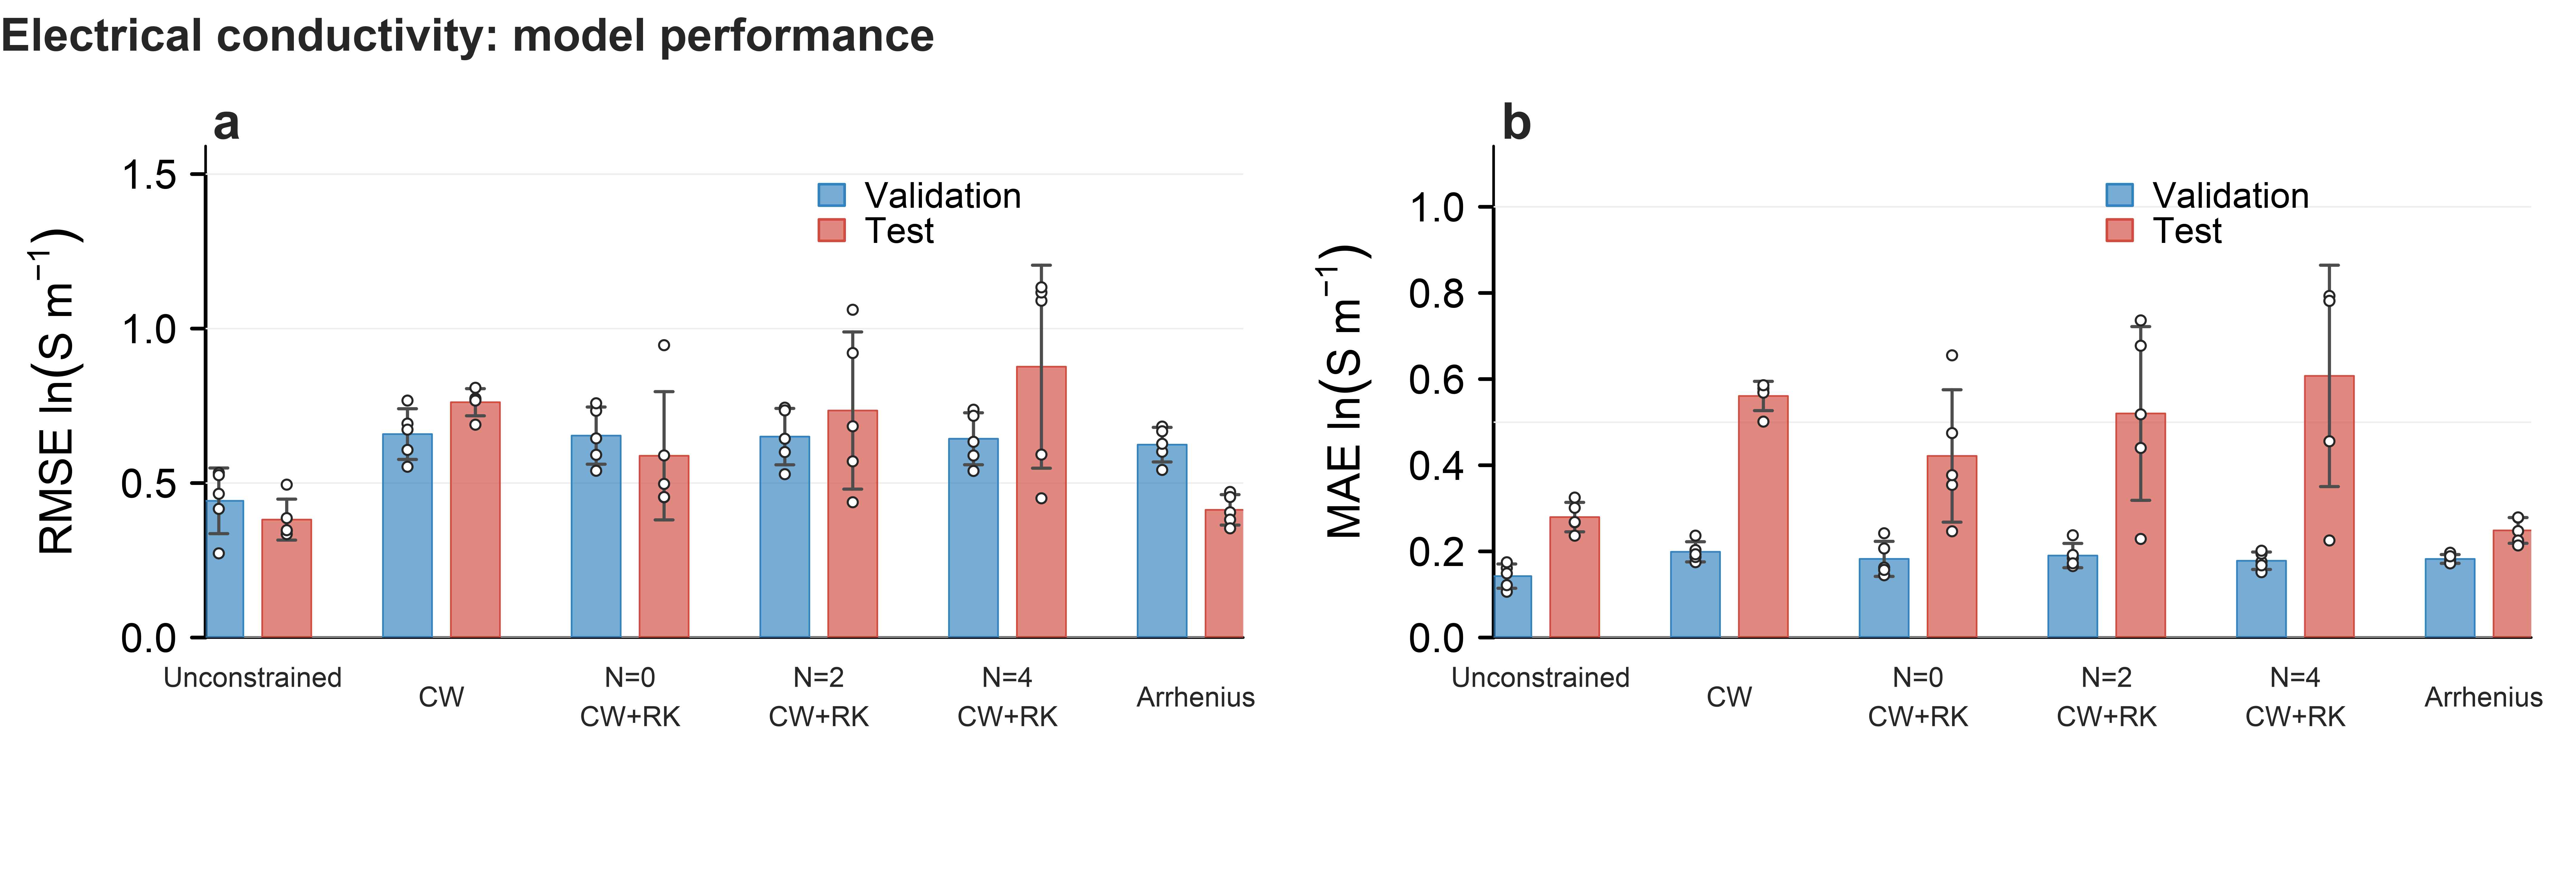
\includegraphics[width=\linewidth,height=0.68\textheight,keepaspectratio]{figures-SI/electrical_conductivity_rmse_mae_by_n.png}
\captionof{figure}{不同模型变体和 RK 阶数下的电导率 RMSE 与 MAE 比较。}
\label{fig:si-electrical-conductivity-rmse-mae}
\end{minipage}
\end{center}

\begin{center}
\begin{minipage}{\linewidth}
\centering
\makebox[\linewidth][c]{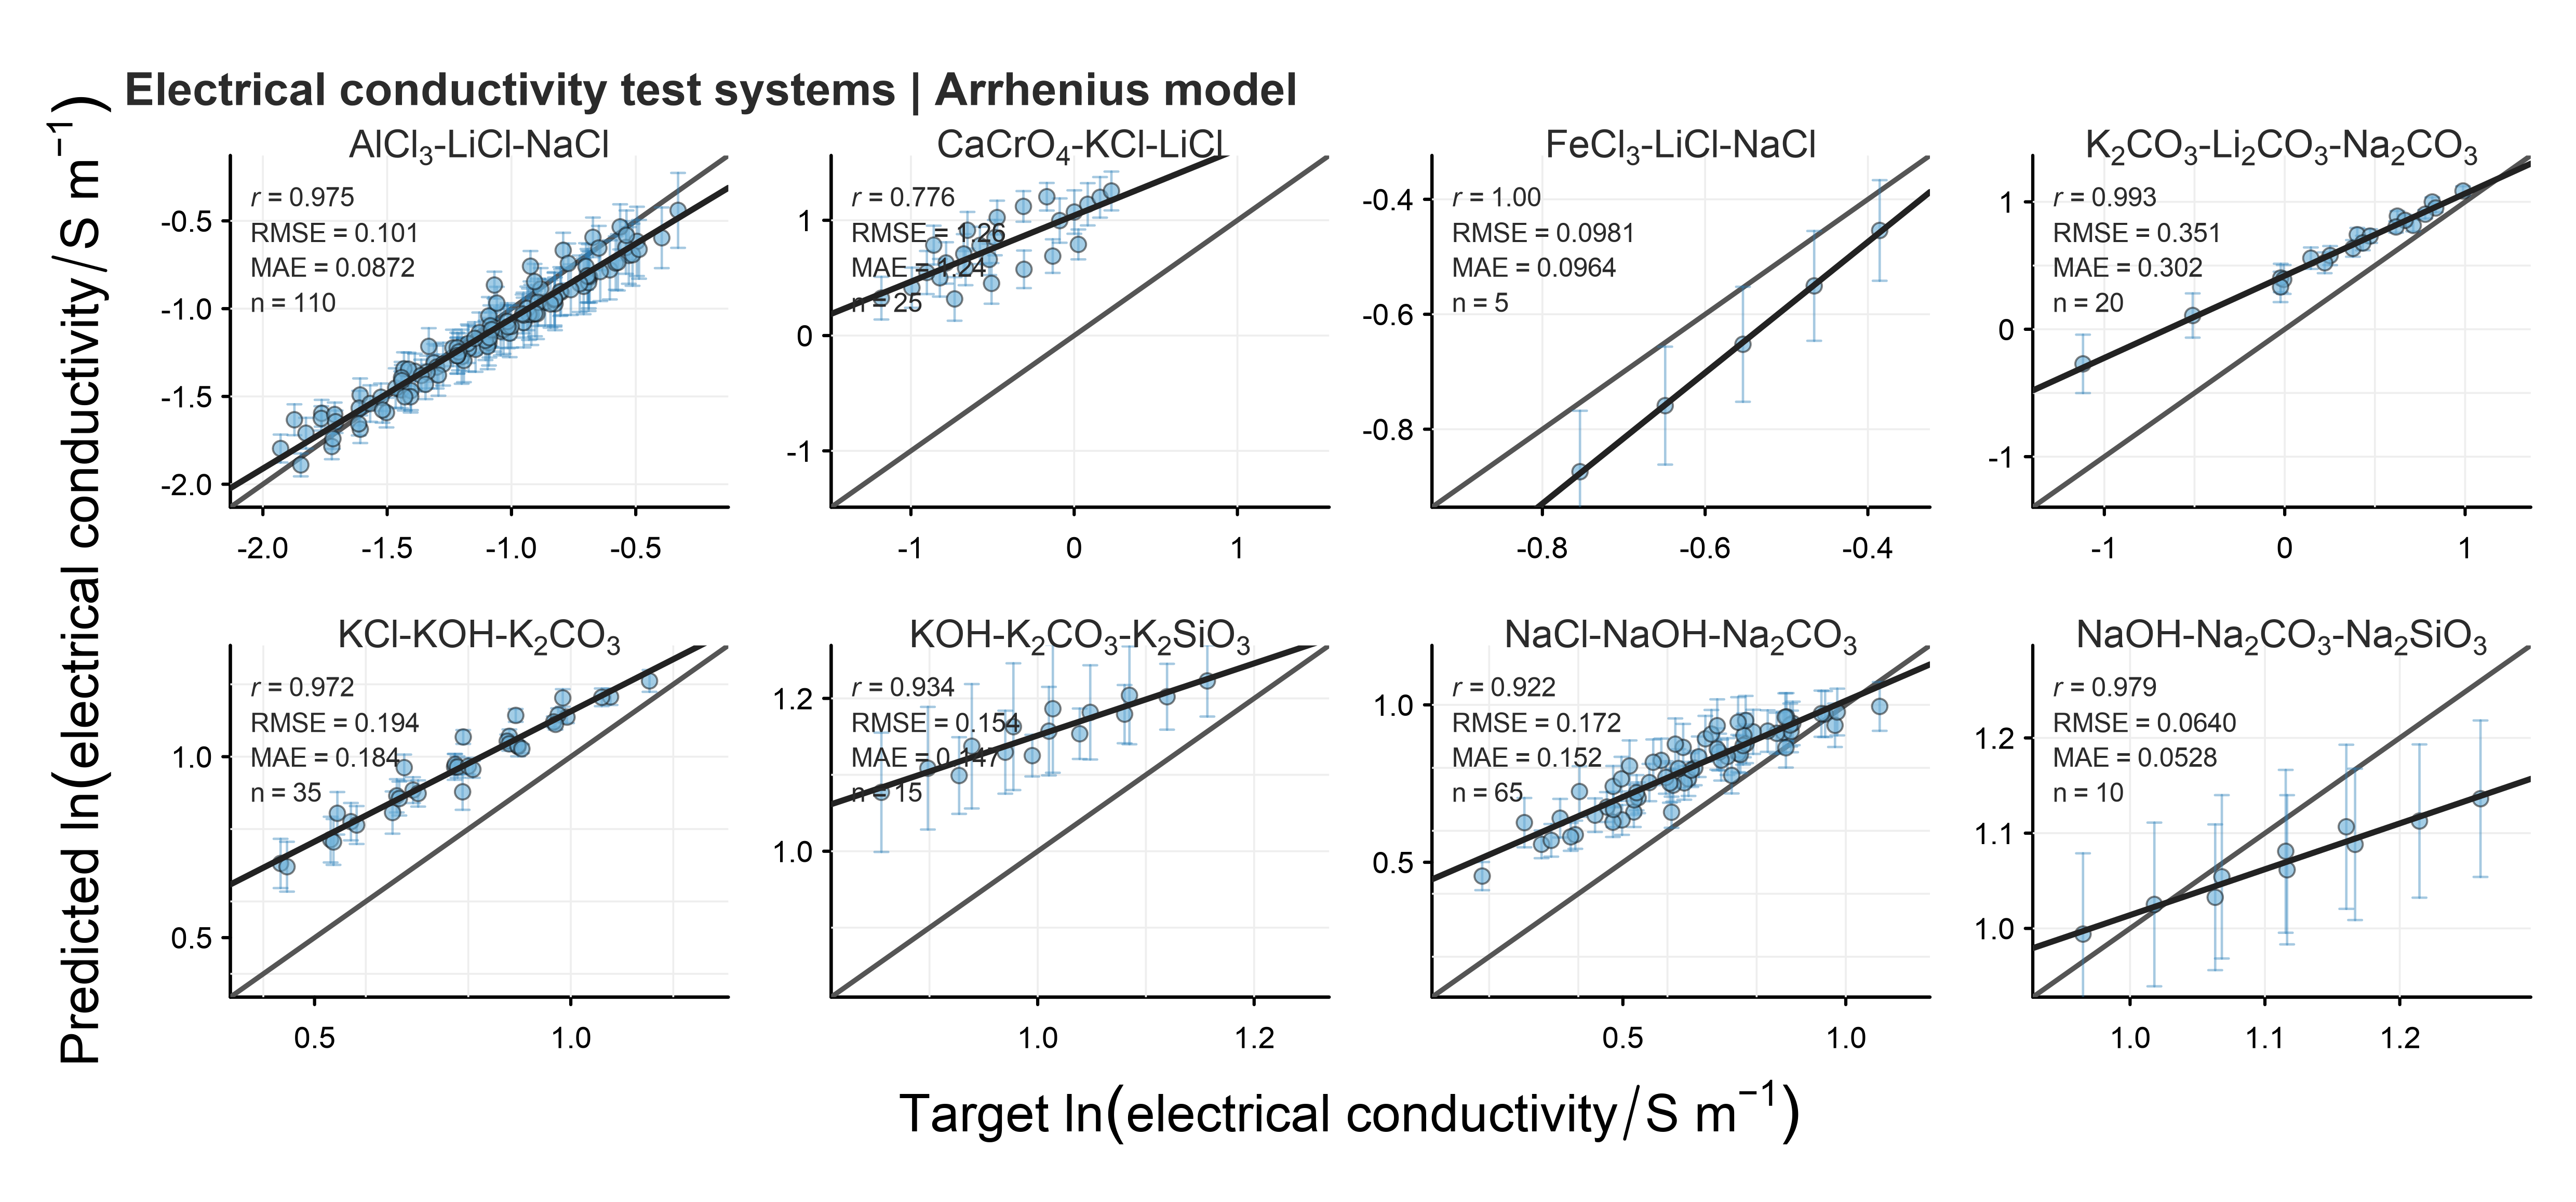
\includegraphics[width=\linewidth]{figures-SI/electrical_conductivity_test_system_correlation_grid_arrhenius_model_page_01.png}}
\captionof{figure}{Arrhenius 约束模型在电导率测试体系中的相关性网格图。}
\label{fig:si-electrical-conductivity-test-correlation}
\end{minipage}
\end{center}

对于电导率，主导性的三元离群体系是 CaCrO\(_4\)--KCl--LiCl，其对数空间 MAE 为 1.235，最大绝对误差为 1.645。模型严重高估该体系，对若干目标值为负的样本预测出正的对数电导率。该失效与严重的低阶覆盖缺口一致：纯 CaCrO\(_4\) 记录缺失，同时 CaCrO\(_4\)--KCl 二元覆盖也缺失，使三元预测只能依赖来自相关组分的稀疏迁移。

其余电导率误差较小，但呈现相同的化学特异性外推模式。K\(_2\)CO\(_3\)--Li\(_2\)CO\(_3\)--Na\(_2\)CO\(_3\) 的一元和二元覆盖完整，但仍被高估（对数空间 MAE = 0.302），尤其是在碳酸盐三元记录的低电导率部分；这表明低阶 Arrhenius 混合未能充分捕捉三元碳酸盐趋势。KCl--KOH--K\(_2\)CO\(_3\)、NaCl--NaOH--Na\(_2\)CO\(_3\)、KOH--K\(_2\)CO\(_3\)--K\(_2\)SiO\(_3\) 和 NaOH--Na\(_2\)CO\(_3\)--Na\(_2\)SiO\(_3\) 主要受到氢氧化物、碳酸盐和硅酸盐二元子体系缺失或稀疏的影响。该测试集中没有四元电导率体系。

\section*{4. 测试体系的子体系覆盖}\label{subsystem-coverage-of-test-systems}

本节汇总密度、表面张力、黏度和电导率任务中测试体系的子体系覆盖情况。测试记录的指标按 RMSE/MAE/r 的顺序给出，其中 Pearson 相关系数 \(r\) 按目标值与预测值的相关性计算。

\subsection*{4.1 密度}\label{density}

模型：CW+RK 模型 \(N=0\)。测试记录指标按 RMSE/MAE/r 的顺序给出，其中 Pearson 相关系数 \(r\) 按目标值与预测值的相关性计算。每个测试体系以纵向行块列出：首先给出目标体系，随后给出可用的密度子体系记录，包括记录编号、摩尔比和温度区间。缺失记录以 \passthrough{\lstinline!-!} 标记。

\subsubsection*{三元体系}\label{ternary-system-2}

{
\silongtablecaption{密度三元测试体系的子体系覆盖。}
\begin{longtable}[]{@{}
  >{\raggedright\arraybackslash}p{(\linewidth - 2\tabcolsep) * \real{0.1600}}
  >{\raggedright\arraybackslash}p{(\linewidth - 2\tabcolsep) * \real{0.8400}}@{}}
\toprule\noalign{}
\begin{minipage}[b]{\linewidth}\raggedright
项目
\end{minipage} & \begin{minipage}[b]{\linewidth}\raggedright
记录
\end{minipage} \\
\midrule\noalign{}
\endhead
\bottomrule\noalign{}
\endlastfoot
体系 & \textbf{AlCl\textsubscript{3}-LiCl-NaCl} \\
 & 记录1： MSTDB\_TP\_V4\_DEN\_0006; 50-10-40 mol\%; 432-606 K; 0.038/0.038/1.000 \\
 & 记录2： MSTDB\_TP\_V4\_DEN\_0007; 50-20-30 mol\%; 419-545 K; 0.046/0.046/1.000 \\
 & 记录3： MSTDB\_TP\_V4\_DEN\_0008; 50-30-20 mol\%; 397-534 K; 0.061/0.061/1.000 \\
 & 记录4： MSTDB\_TP\_V4\_DEN\_0009; 50-40-10 mol\%; 418-535 K; 0.067/0.067/1.000 \\
 & 记录5： MSTDB\_TP\_V4\_DEN\_0010; 60-10-30 mol\%; 426-520 K; 0.006/0.006/1.000 \\
 & 记录6： MSTDB\_TP\_V4\_DEN\_0011; 60-20-20 mol\%; 426-482 K; 0.017/0.017/1.000 \\
 & 记录7： MSTDB\_TP\_V4\_DEN\_0012; 60-30-10 mol\%; 426-500 K; 0.025/0.025/1.000 \\
 & 记录8： MSTDB\_TP\_V4\_DEN\_0013; 70-10-20 mol\%; 464-545 K; 0.037/0.036/1.000 \\
 & 记录9： MSTDB\_TP\_V4\_DEN\_0014; 70-20-10 mol\%; 468-492 K; 0.032/0.032/1.000 \\
 & 记录10： MSTDB\_TP\_V4\_DEN\_0015; 80-10-10 mol\%; 473-492 K; 0.030/0.030/1.000 \\
 & 记录11： EXP\_DEN\_P022\_044; 50-30-20 mol\%; 397-534 K; 0.061/0.061/1.000 \\
 & 记录12： EXP\_DEN\_P022\_045; 50-40-10 mol\%; 418-535 K; 0.070/0.070/1.000 \\
 & 记录13： EXP\_DEN\_P022\_046; 50-20-30 mol\%; 419-545 K; 0.049/0.049/1.000 \\
 & 记录14： EXP\_DEN\_P022\_047; 50-10-40 mol\%; 432-606 K; 0.035/0.035/1.000 \\
 & 记录15： EXP\_DEN\_P022\_048; 60-20-20 mol\%; 426-482 K; 0.020/0.020/1.000 \\
 & 记录16： EXP\_DEN\_P022\_049; 60-30-10 mol\%; 426-500 K; 0.029/0.029/1.000 \\
 & 记录17： EXP\_DEN\_P022\_050; 60-10-30 mol\%; 426-520 K; 0.011/0.011/1.000 \\
 & 记录18： EXP\_DEN\_P023\_001; 69.7-20.2-10.1 mol\%; 468-492 K; 0.032/0.032/1.000 \\
 & 记录19： EXP\_DEN\_P023\_002; 69.8-10.1-20.1 mol\%; 464-545 K; 0.053/0.052/1.000 \\
 & 记录20： EXP\_DEN\_P023\_003; 69.9-20.0-10.1 mol\%; 464-535 K; 0.027/0.027/1.000 \\
 & 记录21： EXP\_DEN\_P023\_004; 79.2-10.4-10.4 mol\%; 463-515 K; 0.068/0.067/1.000 \\
 & 记录22： EXP\_DEN\_P023\_005; 79.9-10.0-10.1 mol\%; 473-492 K; 0.022/0.022/1.000 \\
 & 总体： 0.042/0.038/0.920  \\

组分 1  & \textbf{AlCl\textsubscript{3}} \\
 & 记录1： MSTDB\_TP\_V4\_DEN\_0001; 100 mol\%; 462-569 K \\
 & 记录2： EXP\_DEN\_P022\_023; 100 mol\%; 462-569 K  \\

组分 2  & \textbf{LiCl} \\
 & 记录1： MSTDB\_TP\_V4\_DEN\_0362; 100 mol\%; 893.2-1053.2 K \\
 & 记录2： EXP\_DEN\_P068\_001; 100 mol\%; 894-1054 K  \\

组分 3  & \textbf{NaCl} \\
 & 记录1： MSTDB\_TP\_V4\_DEN\_0519; 100 mol\%; 1076.2-1303.2 K \\
 & 记录2： EXP\_DEN\_P078\_001; 100 mol\%; 1080-1300 K  \\

二元子体系 1  & \textbf{AlCl\textsubscript{3}-LiCl} \\
 & 记录1： EXP\_DEN\_P022\_033; 49.25-50.75 mol\%; 420-530 K \\
 & 记录2： EXP\_DEN\_P022\_034; 54.7-45.3 mol\%; 470-520 K \\
 & 记录3： EXP\_DEN\_P022\_035; 55-45 mol\%; 450-495 K \\
 & 记录4： EXP\_DEN\_P022\_036; 60-40 mol\%; 450-495 K \\
 & 记录5： EXP\_DEN\_P022\_037; 60-40 mol\%; 470-540 K \\
 & 记录6： EXP\_DEN\_P022\_038; 65-35 mol\%; 450-495 K \\
 & 记录7： EXP\_DEN\_P022\_039; 65.3-34.7 mol\%; 470-540 K \\
 & 记录8： EXP\_DEN\_P022\_040; 69.8-30.2 mol\%; 470-520 K \\
 & 记录9： EXP\_DEN\_P022\_041; 70-30 mol\%; 450-495 K \\
 & 记录10： EXP\_DEN\_P022\_042; 75-25 mol\%; 470-520 K \\
 & 记录11： EXP\_DEN\_P022\_043; 75.0-25.0 mol\%; 450-495 K  \\

二元子体系 2  & \textbf{AlCl\textsubscript{3}-NaCl} \\
 & 记录1： MSTDB\_TP\_V4\_DEN\_0016; 52-48 mol\%; 400-560 K \\
 & 记录2： MSTDB\_TP\_V4\_DEN\_0017; 61.8-38.2 mol\%; 440-540 K \\
 & 记录3： MSTDB\_TP\_V4\_DEN\_0018; 73-27 mol\%; 460-610 K \\
 & 记录4： EXP\_DEN\_P023\_012; 52.0-48.0 mol\%; 400-560 K \\
 & 记录5： EXP\_DEN\_P023\_013; 61.8-38.2 mol\%; 440-540 K \\
 & 记录6： EXP\_DEN\_P023\_014; 73.0-27.0 mol\%; 460-610 K \\
 & 记录7： EXP\_DEN\_P023\_015; 100-0 mol\%; 480-490 K  \\

二元子体系 3  & \textbf{LiCl-NaCl} \\
 & 记录1： MSTDB\_TP\_V4\_DEN\_0363; 10-90 mol\%; 880-1115 K \\
 & 记录2： MSTDB\_TP\_V4\_DEN\_0364; 20-80 mol\%; 863-1110 K \\
 & 记录3： MSTDB\_TP\_V4\_DEN\_0365; 30-70 mol\%; 850-1100 K \\
 & 记录4： MSTDB\_TP\_V4\_DEN\_0366; 50-50 mol\%; 901-1143 K \\
 & 记录5： MSTDB\_TP\_V4\_DEN\_0367; 70-30 mol\%; 980-1207 K \\
 & 记录6： MSTDB\_TP\_V4\_DEN\_0368; 80-20 mol\%; 1045-1255 K \\
 & 记录7： EXP\_DEN\_P068\_043; 0-100 mol\%; 1090-1220 K \\
 & 记录8： EXP\_DEN\_P068\_044; 50-50 mol\%; 900-1120 K \\
 & 记录9： EXP\_DEN\_P069\_001; 100-0 mol\%; 880-1070 K  \\

\midrule
体系 & \textbf{BeF\textsubscript{2}-KF-NaF} \\
 & 记录1： MSTDB\_TP\_V4\_DEN\_0023; 36-15-49 mol\%; 828-1273 K; 0.028/0.022/1.000 \\
 & 总体： 0.028/0.022/1.000  \\

组分 1  & \textbf{BeF\textsubscript{2}} \\
 & 记录1： MSTDB\_TP\_V4\_DEN\_0020; 100 mol\%; 1080-1170 K \\
 & 记录2： EXP\_DEN\_P028\_030; 100 mol\%; 1073-1123 K  \\

组分 2  & \textbf{KF} \\
 & 记录1： MSTDB\_TP\_V4\_DEN\_0328; 100 mol\%; 1143-1283 K \\
 & 记录2： EXP\_DEN\_P056\_006; 100 mol\%; 1154-1310 K  \\

组分 3  & \textbf{NaF} \\
 & 记录1： MSTDB\_TP\_V4\_DEN\_0589; 100 mol\%; 1273-1473 K \\
 & 记录2： EXP\_DEN\_P081\_037; 100 mol\%; 1280-1370 K  \\

二元子体系 1  & \textbf{BeF\textsubscript{2}-KF} \\
 & 记录1： MSTDB\_TP\_V4\_DEN\_0021; 21-79 mol\%; 1003-1273 K \\
 & 记录2： MSTDB\_TP\_V4\_DEN\_0022; 50-50 mol\%; 718-1273 K  \\

二元子体系 2  & \textbf{BeF\textsubscript{2}-NaF} \\
 & 记录1： MSTDB\_TP\_V4\_DEN\_0076; 30-70 mol\%; 873-1073 K \\
 & 记录2： MSTDB\_TP\_V4\_DEN\_0077; 33.3-66.7 mol\%; 873-1073 K \\
 & 记录3： MSTDB\_TP\_V4\_DEN\_0078; 36-64 mol\%; 873-1073 K \\
 & 记录4： MSTDB\_TP\_V4\_DEN\_0079; 40-60 mol\%; 873-1073 K \\
 & 记录5： MSTDB\_TP\_V4\_DEN\_0080; 42-58 mol\%; 873-1073 K \\
 & 记录6： MSTDB\_TP\_V4\_DEN\_0081; 47.1-52.9 mol\%; 873-1073 K \\
 & 记录7： MSTDB\_TP\_V4\_DEN\_0082; 48-52 mol\%; 873-1073 K \\
 & 记录8： MSTDB\_TP\_V4\_DEN\_0083; 50-50 mol\%; 873-1073 K \\
 & 记录9： MSTDB\_TP\_V4\_DEN\_0084; 54-46 mol\%; 873-1073 K \\
 & 记录10： MSTDB\_TP\_V4\_DEN\_0085; 60-40 mol\%; 873-1073 K \\
 & 记录11： EXP\_DEN\_P029\_001; 20-80 mol\%; 1073 K \\
 & 记录12： EXP\_DEN\_P029\_002; 24-76 mol\%; 1073 K \\
 & 记录13： EXP\_DEN\_P029\_003; 30-70 mol\%; 873-1073 K \\
 & 记录14： EXP\_DEN\_P029\_004; 33.3-66.7 mol\%; 873-1073 K \\
 & 记录15： EXP\_DEN\_P029\_005; 36-64 mol\%; 873-1073 K \\
 & 记录16： EXP\_DEN\_P029\_006; 40-60 mol\%; 873-1073 K \\
 & 记录17： EXP\_DEN\_P029\_007; 42-58 mol\%; 873-1073 K \\
 & 记录18： EXP\_DEN\_P029\_008; 47.1-52.9 mol\%; 873-1073 K \\
 & 记录19： EXP\_DEN\_P029\_009; 48-52 mol\%; 873-1073 K \\
 & 记录20： EXP\_DEN\_P029\_010; 50-50 mol\%; 873-1073 K \\
 & 记录21： EXP\_DEN\_P029\_011; 54-46 mol\%; 873-1073 K \\
 & 记录22： EXP\_DEN\_P029\_012; 60-40 mol\%; 873-1073 K \\
 & 记录23： EXP\_DEN\_P029\_013; 80-20 mol\%; 1073 K  \\

二元子体系 3  & \textbf{KF-NaF} \\
 & 记录1： MSTDB\_TP\_V4\_DEN\_0338; 20-80 mol\%; 1200-1350 K \\
 & 记录2： MSTDB\_TP\_V4\_DEN\_0339; 40-60 mol\%; 1125-1350 K \\
 & 记录3： MSTDB\_TP\_V4\_DEN\_0340; 60-40 mol\%; 1050-1250 K \\
 & 记录4： MSTDB\_TP\_V4\_DEN\_0341; 75-25 mol\%; 1065-1350 K \\
 & 记录5： MSTDB\_TP\_V4\_DEN\_0342; 88-12 mol\%; 1095-1350 K \\
 & 记录6： EXP\_DEN\_P057\_001; 0.0-100.0 mol\%; 1275-1350 K \\
 & 记录7： EXP\_DEN\_P057\_002; 20.0-80.0 mol\%; 1200-1350 K \\
 & 记录8： EXP\_DEN\_P057\_003; 40.0-60.0 mol\%; 1125-1350 K \\
 & 记录9： EXP\_DEN\_P057\_004; 60.0-40.0 mol\%; 1050-1350 K \\
 & 记录10： EXP\_DEN\_P057\_005; 75.0-25.0 mol\%; 1065-1350 K \\
 & 记录11： EXP\_DEN\_P057\_006; 88.0-12.0 mol\%; 1095-1350 K \\
 & 记录12： EXP\_DEN\_P057\_007; 100.0-0.0 mol\%; 1140-1350 K  \\

\midrule
体系 & \textbf{BeF\textsubscript{2}-LiF-NaF} \\
 & 记录1： MSTDB\_TP\_V4\_DEN\_0028; 15-36-49 mol\%; 870-1273 K; 0.063/0.061/1.000 \\
 & 记录2： MSTDB\_TP\_V4\_DEN\_0029; 23-24-53 mol\%; 808-1273 K; 0.025/0.021/0.999 \\
 & 记录3： MSTDB\_TP\_V4\_DEN\_0030; 28-16-56 mol\%; 751-1273 K; 0.143/0.142/0.999 \\
 & 记录4： MSTDB\_TP\_V4\_DEN\_0031; 31-5-64 mol\%; 828-1273 K; 0.053/0.053/1.000 \\
 & 总体： 0.084/0.069/0.611  \\

组分 1  & \textbf{BeF\textsubscript{2}} \\
 & 记录1： MSTDB\_TP\_V4\_DEN\_0020; 100 mol\%; 1080-1170 K \\
 & 记录2： EXP\_DEN\_P028\_030; 100 mol\%; 1073-1123 K  \\

组分 2  & \textbf{LiF} \\
 & 记录1： MSTDB\_TP\_V4\_DEN\_0455; 100 mol\%; 1123.6-1367.5 K \\
 & 记录2： EXP\_DEN\_P070\_030; 100 mol\%; 1149-1320 K  \\

组分 3  & \textbf{NaF} \\
 & 记录1： MSTDB\_TP\_V4\_DEN\_0589; 100 mol\%; 1273-1473 K \\
 & 记录2： EXP\_DEN\_P081\_037; 100 mol\%; 1280-1370 K  \\

二元子体系 1  & \textbf{BeF\textsubscript{2}-LiF} \\
 & 记录1： MSTDB\_TP\_V4\_DEN\_0024; 34-66 mol\%; 787.7-1093.5 K \\
 & 记录2： MSTDB\_TP\_V4\_DEN\_0025; 50-50 mol\%; 800-1080 K \\
 & 记录3： MSTDB\_TP\_V4\_DEN\_0026; 75-25 mol\%; 860-1130 K \\
 & 记录4： MSTDB\_TP\_V4\_DEN\_0027; 89-11 mol\%; 1020-1130 K \\
 & 记录5： EXP\_DEN\_P028\_031; 34.0-66.0 mol\%; 800-1080 K \\
 & 记录6： EXP\_DEN\_P028\_032; 50.2-49.8 mol\%; 930-1130 K \\
 & 记录7： EXP\_DEN\_P028\_033; 74.9-25.1 mol\%; 860-1130 K \\
 & 记录8： EXP\_DEN\_P028\_034; 89.2-10.8 mol\%; 1020-1130 K  \\

二元子体系 2  & \textbf{BeF\textsubscript{2}-NaF} \\
 & 记录1： MSTDB\_TP\_V4\_DEN\_0076; 30-70 mol\%; 873-1073 K \\
 & 记录2： MSTDB\_TP\_V4\_DEN\_0077; 33.3-66.7 mol\%; 873-1073 K \\
 & 记录3： MSTDB\_TP\_V4\_DEN\_0078; 36-64 mol\%; 873-1073 K \\
 & 记录4： MSTDB\_TP\_V4\_DEN\_0079; 40-60 mol\%; 873-1073 K \\
 & 记录5： MSTDB\_TP\_V4\_DEN\_0080; 42-58 mol\%; 873-1073 K \\
 & 记录6： MSTDB\_TP\_V4\_DEN\_0081; 47.1-52.9 mol\%; 873-1073 K \\
 & 记录7： MSTDB\_TP\_V4\_DEN\_0082; 48-52 mol\%; 873-1073 K \\
 & 记录8： MSTDB\_TP\_V4\_DEN\_0083; 50-50 mol\%; 873-1073 K \\
 & 记录9： MSTDB\_TP\_V4\_DEN\_0084; 54-46 mol\%; 873-1073 K \\
 & 记录10： MSTDB\_TP\_V4\_DEN\_0085; 60-40 mol\%; 873-1073 K \\
 & 记录11： EXP\_DEN\_P029\_001; 20-80 mol\%; 1073 K \\
 & 记录12： EXP\_DEN\_P029\_002; 24-76 mol\%; 1073 K \\
 & 记录13： EXP\_DEN\_P029\_003; 30-70 mol\%; 873-1073 K \\
 & 记录14： EXP\_DEN\_P029\_004; 33.3-66.7 mol\%; 873-1073 K \\
 & 记录15： EXP\_DEN\_P029\_005; 36-64 mol\%; 873-1073 K \\
 & 记录16： EXP\_DEN\_P029\_006; 40-60 mol\%; 873-1073 K \\
 & 记录17： EXP\_DEN\_P029\_007; 42-58 mol\%; 873-1073 K \\
 & 记录18： EXP\_DEN\_P029\_008; 47.1-52.9 mol\%; 873-1073 K \\
 & 记录19： EXP\_DEN\_P029\_009; 48-52 mol\%; 873-1073 K \\
 & 记录20： EXP\_DEN\_P029\_010; 50-50 mol\%; 873-1073 K \\
 & 记录21： EXP\_DEN\_P029\_011; 54-46 mol\%; 873-1073 K \\
 & 记录22： EXP\_DEN\_P029\_012; 60-40 mol\%; 873-1073 K \\
 & 记录23： EXP\_DEN\_P029\_013; 80-20 mol\%; 1073 K  \\

二元子体系 3  & \textbf{LiF-NaF} \\
 & 记录1： MSTDB\_TP\_V4\_DEN\_0456; 10-90 mol\%; 1280-1320 K \\
 & 记录2： MSTDB\_TP\_V4\_DEN\_0457; 20-80 mol\%; 1280-1320 K \\
 & 记录3： MSTDB\_TP\_V4\_DEN\_0458; 30-70 mol\%; 1230-1320 K \\
 & 记录4： MSTDB\_TP\_V4\_DEN\_0459; 40-60 mol\%; 1130-1320 K \\
 & 记录5： MSTDB\_TP\_V4\_DEN\_0460; 50-50 mol\%; 1130-1320 K \\
 & 记录6： MSTDB\_TP\_V4\_DEN\_0461; 60-40 mol\%; 1130-1320 K \\
 & 记录7： MSTDB\_TP\_V4\_DEN\_0462; 70-30 mol\%; 1130-1320 K \\
 & 记录8： MSTDB\_TP\_V4\_DEN\_0463; 80-20 mol\%; 1130-1320 K \\
 & 记录9： MSTDB\_TP\_V4\_DEN\_0464; 90-10 mol\%; 1130-1320 K \\
 & 记录10： EXP\_DEN\_P070\_036; 0-100 mol\%; 1280-1320 K \\
 & 记录11： EXP\_DEN\_P070\_037; 10-90 mol\%; 1280-1320 K \\
 & 记录12： EXP\_DEN\_P070\_038; 20-80 mol\%; 1230-1320 K \\
 & 记录13： EXP\_DEN\_P070\_039; 30-70 mol\%; 1130-1320 K \\
 & 记录14： EXP\_DEN\_P070\_040; 40-60 mol\%; 1130-1320 K \\
 & 记录15： EXP\_DEN\_P071\_001; 50-50 mol\%; 1130-1320 K \\
 & 记录16： EXP\_DEN\_P071\_002; 60-40 mol\%; 1130-1320 K \\
 & 记录17： EXP\_DEN\_P071\_003; 70-30 mol\%; 1130-1320 K \\
 & 记录18： EXP\_DEN\_P071\_004; 80-20 mol\%; 1130-1320 K \\
 & 记录19： EXP\_DEN\_P071\_005; 90-10 mol\%; 1130-1320 K \\
 & 记录20： EXP\_DEN\_P071\_006; 100-0 mol\%; 1130-1320 K  \\

\midrule
体系 & \textbf{BeF\textsubscript{2}-LiF-ThF\textsubscript{4}} \\
 & 记录1： MSTDB\_TP\_V4\_DEN\_0034; 14.99-69.98-15.03 mol\%; 816.6-1022.7 K; 0.119/0.118/1.000 \\
 & 记录2： MSTDB\_TP\_V4\_DEN\_0035; 17.96-70.06-11.98 mol\%; 806.4-1014.4 K; 0.134/0.134/1.000 \\
 & 记录3： MSTDB\_TP\_V4\_DEN\_0036; 23.88-70.11-6.01 mol\%; 828.3-980.6 K; 0.083/0.083/1.000 \\
 & 记录4： EXP\_DEN\_P028\_035; 15-70-15 mol\%; 830-1010 K; 0.123/0.122/1.000 \\
 & 记录5： EXP\_DEN\_P028\_036; 18-70-12 mol\%; 800-1010 K; 0.138/0.138/1.000 \\
 & 记录6： EXP\_DEN\_P028\_037; 23.9-70.1-6.0 mol\%; 830-980 K; 0.079/0.079/1.000 \\
 & 总体： 0.115/0.112/0.999  \\

组分 1  & \textbf{BeF\textsubscript{2}} \\
 & 记录1： MSTDB\_TP\_V4\_DEN\_0020; 100 mol\%; 1080-1170 K \\
 & 记录2： EXP\_DEN\_P028\_030; 100 mol\%; 1073-1123 K  \\

组分 2  & \textbf{LiF} \\
 & 记录1： MSTDB\_TP\_V4\_DEN\_0455; 100 mol\%; 1123.6-1367.5 K \\
 & 记录2： EXP\_DEN\_P070\_030; 100 mol\%; 1149-1320 K  \\

组分 3  & \textbf{ThF\textsubscript{4}} \\
 & 记录1： MSTDB\_TP\_V4\_DEN\_0621; 100 mol\%; 1393-1651 K \\
 & 记录2： EXP\_DEN\_P096\_002; 100 mol\%; 1393-1651 K  \\

二元子体系 1  & \textbf{BeF\textsubscript{2}-LiF} \\
 & 记录1： MSTDB\_TP\_V4\_DEN\_0024; 34-66 mol\%; 787.7-1093.5 K \\
 & 记录2： MSTDB\_TP\_V4\_DEN\_0025; 50-50 mol\%; 800-1080 K \\
 & 记录3： MSTDB\_TP\_V4\_DEN\_0026; 75-25 mol\%; 860-1130 K \\
 & 记录4： MSTDB\_TP\_V4\_DEN\_0027; 89-11 mol\%; 1020-1130 K \\
 & 记录5： EXP\_DEN\_P028\_031; 34.0-66.0 mol\%; 800-1080 K \\
 & 记录6： EXP\_DEN\_P028\_032; 50.2-49.8 mol\%; 930-1130 K \\
 & 记录7： EXP\_DEN\_P028\_033; 74.9-25.1 mol\%; 860-1130 K \\
 & 记录8： EXP\_DEN\_P028\_034; 89.2-10.8 mol\%; 1020-1130 K  \\

二元子体系 2 & \textbf{BeF\textsubscript{2}-ThF\textsubscript{4}} \\
 & 记录1： 无 \\
二元子体系 3  & \textbf{LiF-ThF\textsubscript{4}} \\
 & 记录1： MSTDB\_TP\_V4\_DEN\_0476; 20-80 mol\%; 1320-1440 K \\
 & 记录2： MSTDB\_TP\_V4\_DEN\_0477; 40-60 mol\%; 1220-1360 K \\
 & 记录3： MSTDB\_TP\_V4\_DEN\_0478; 60-40 mol\%; 1080-1260 K \\
 & 记录4： MSTDB\_TP\_V4\_DEN\_0479; 80-20 mol\%; 1020-1220 K \\
 & 记录5： MSTDB\_TP\_V4\_DEN\_0480; 81.36-18.64 mol\%; 1040-1220 K \\
 & 记录6： EXP\_DEN\_P071\_022; 0-100 mol\%; 1400-1500 K \\
 & 记录7： EXP\_DEN\_P071\_023; 20.00-80.00 mol\%; 1320-1440 K \\
 & 记录8： EXP\_DEN\_P071\_024; 40.0-60.0 mol\%; 1220-1360 K \\
 & 记录9： EXP\_DEN\_P071\_025; 60.00-40.00 mol\%; 1080-1260 K \\
 & 记录10： EXP\_DEN\_P071\_026; 80.00-20.00 mol\%; 1020-1220 K \\
 & 记录11： EXP\_DEN\_P071\_027; 81.36-18.64 mol\%; 1040-1220 K \\
 & 记录12： EXP\_DEN\_P071\_028; 100.0-0.0 mol\%; 1140-1360 K  \\

\midrule
体系 & \textbf{BeF\textsubscript{2}-LiF-UF\textsubscript{4}} \\
 & 记录1： MSTDB\_TP\_V4\_DEN\_0038; 5-60-35 mol\%; 973-1073 K; 0.231/0.230/0.999 \\
 & 记录2： MSTDB\_TP\_V4\_DEN\_0039; 10-70-20 mol\%; 873-1073 K; 0.110/0.107/0.999 \\
 & 记录3： MSTDB\_TP\_V4\_DEN\_0040; 12-76-12 mol\%; 873-1073 K; 0.023/0.019/1.000 \\
 & 记录4： MSTDB\_TP\_V4\_DEN\_0041; 12-80-8 mol\%; 973-1073 K; 0.007/0.006/1.000 \\
 & 记录5： MSTDB\_TP\_V4\_DEN\_0042; 14-80-6 mol\%; 973-1073 K; 0.088/0.088/1.000 \\
 & 记录6： MSTDB\_TP\_V4\_DEN\_0043; 15-50-35 mol\%; 973-1073 K; 0.407/0.407/0.999 \\
 & 记录7： MSTDB\_TP\_V4\_DEN\_0044; 18-70-12 mol\%; 873-1073 K; 0.020/0.018/1.000 \\
 & 记录8： MSTDB\_TP\_V4\_DEN\_0045; 18-80-2 mol\%; 973-1073 K; 0.110/0.110/1.000 \\
 & 记录9： MSTDB\_TP\_V4\_DEN\_0046; 20-60-20 mol\%; 873-1073 K; 0.160/0.158/1.000 \\
 & 记录10： MSTDB\_TP\_V4\_DEN\_0047; 21-75-4 mol\%; 873-1073 K; 0.106/0.106/1.000 \\
 & 记录11： MSTDB\_TP\_V4\_DEN\_0048; 22-70-8 mol\%; 873-1073 K; 0.015/0.013/1.000 \\
 & 记录12： MSTDB\_TP\_V4\_DEN\_0049; 23-75-2 mol\%; 873-1073 K; 0.081/0.080/1.000 \\
 & 记录13： MSTDB\_TP\_V4\_DEN\_0050; 24-70-6 mol\%; 873-973 K; 0.088/0.088/1.000 \\
 & 记录14： MSTDB\_TP\_V4\_DEN\_0051; 25-40-35 mol\%; 973-1073 K; 0.262/0.262/1.000 \\
 & 记录15： MSTDB\_TP\_V4\_DEN\_0052; 26-70-4 mol\%; 873-1073 K; 0.081/0.081/1.000 \\
 & 记录16： MSTDB\_TP\_V4\_DEN\_0053; 28-60-12 mol\%; 873-1073 K; 0.011/0.009/1.000 \\
 & 记录17： MSTDB\_TP\_V4\_DEN\_0054; 28-70-2 mol\%; 873-1073 K; 0.103/0.103/1.000 \\
 & 记录18： MSTDB\_TP\_V4\_DEN\_0055; 30-50-20 mol\%; 873-1073 K; 0.121/0.120/1.000 \\
 & 记录19： MSTDB\_TP\_V4\_DEN\_0056; 31-65-4 mol\%; 873-1073 K; 0.102/0.102/1.000 \\
 & 记录20： MSTDB\_TP\_V4\_DEN\_0057; 32-60-8 mol\%; 873-1073 K; 0.095/0.095/1.000 \\
 & 记录21： MSTDB\_TP\_V4\_DEN\_0058; 33-65-2 mol\%; 873-1073 K; 0.093/0.093/1.000 \\
 & 记录22： MSTDB\_TP\_V4\_DEN\_0059; 36-60-4 mol\%; 873-1073 K; 0.110/0.110/1.000 \\
 & 记录23： MSTDB\_TP\_V4\_DEN\_0060; 38-50-12 mol\%; 873-1073 K; 0.034/0.032/1.000 \\
 & 记录24： MSTDB\_TP\_V4\_DEN\_0061; 38-60-2 mol\%; 873-1073 K; 0.113/0.113/1.000 \\
 & 记录25： MSTDB\_TP\_V4\_DEN\_0062; 40-40-20 mol\%; 973-1073 K; 0.102/0.101/1.000 \\
 & 记录26： MSTDB\_TP\_V4\_DEN\_0063; 41-55-4 mol\%; 873-1073 K; 0.091/0.091/1.000 \\
 & 记录27： MSTDB\_TP\_V4\_DEN\_0064; 42-50-8 mol\%; 873-1073 K; 0.054/0.054/1.000 \\
 & 记录28： MSTDB\_TP\_V4\_DEN\_0065; 43-55-2 mol\%; 873-1073 K; 0.108/0.108/1.000 \\
 & 记录29： MSTDB\_TP\_V4\_DEN\_0066; 44-50-6 mol\%; 873-1073 K; 0.055/0.055/1.000 \\
 & 记录30： MSTDB\_TP\_V4\_DEN\_0067; 46-46-8 mol\%; 873-1073 K; 0.074/0.073/1.000 \\
 & 记录31： MSTDB\_TP\_V4\_DEN\_0068; 46-50-4 mol\%; 873-1073 K; 0.087/0.087/1.000 \\
 & 记录32： MSTDB\_TP\_V4\_DEN\_0069; 48-50-2 mol\%; 873-1073 K; 0.128/0.128/1.000 \\
 & 记录33： MSTDB\_TP\_V4\_DEN\_0070; 51-45-4 mol\%; 873-1073 K; 0.089/0.088/1.000 \\
 & 记录34： MSTDB\_TP\_V4\_DEN\_0071; 52-40-8 mol\%; 873-1073 K; 0.094/0.093/1.000 \\
 & 记录35： MSTDB\_TP\_V4\_DEN\_0072; 56-40-4 mol\%; 873-1073 K; 0.136/0.136/1.000 \\
 & 记录36： MSTDB\_TP\_V4\_DEN\_0073; 61-35-4 mol\%; 873-1073 K; 0.136/0.136/1.000 \\
 & 总体： 0.127/0.103/0.996  \\

组分 1  & \textbf{BeF\textsubscript{2}} \\
 & 记录1： MSTDB\_TP\_V4\_DEN\_0020; 100 mol\%; 1080-1170 K \\
 & 记录2： EXP\_DEN\_P028\_030; 100 mol\%; 1073-1123 K  \\

组分 2  & \textbf{LiF} \\
 & 记录1： MSTDB\_TP\_V4\_DEN\_0455; 100 mol\%; 1123.6-1367.5 K \\
 & 记录2： EXP\_DEN\_P070\_030; 100 mol\%; 1149-1320 K  \\

组分 3  & \textbf{UF\textsubscript{4}} \\
 & 记录1： MSTDB\_TP\_V4\_DEN\_0635; 100 mol\%; 1309-1614 K \\
 & 记录2： EXP\_DEN\_P097\_023; 100 mol\%; 1309-1614 K  \\

二元子体系 1  & \textbf{BeF\textsubscript{2}-LiF} \\
 & 记录1： MSTDB\_TP\_V4\_DEN\_0024; 34-66 mol\%; 787.7-1093.5 K \\
 & 记录2： MSTDB\_TP\_V4\_DEN\_0025; 50-50 mol\%; 800-1080 K \\
 & 记录3： MSTDB\_TP\_V4\_DEN\_0026; 75-25 mol\%; 860-1130 K \\
 & 记录4： MSTDB\_TP\_V4\_DEN\_0027; 89-11 mol\%; 1020-1130 K \\
 & 记录5： EXP\_DEN\_P028\_031; 34.0-66.0 mol\%; 800-1080 K \\
 & 记录6： EXP\_DEN\_P028\_032; 50.2-49.8 mol\%; 930-1130 K \\
 & 记录7： EXP\_DEN\_P028\_033; 74.9-25.1 mol\%; 860-1130 K \\
 & 记录8： EXP\_DEN\_P028\_034; 89.2-10.8 mol\%; 1020-1130 K  \\

二元子体系 2  & \textbf{BeF\textsubscript{2}-UF\textsubscript{4}} \\
 & 记录1： EXP\_DEN\_P029\_016; 65-35 mol\%; 1073.2 K  \\

二元子体系 3  & \textbf{LiF-UF\textsubscript{4}} \\
 & 记录1： MSTDB\_TP\_V4\_DEN\_0482; 40-60 mol\%; 1100-1340 K \\
 & 记录2： MSTDB\_TP\_V4\_DEN\_0483; 50-50 mol\%; 1040-1340 K \\
 & 记录3： MSTDB\_TP\_V4\_DEN\_0484; 60-40 mol\%; 980-1340 K \\
 & 记录4： MSTDB\_TP\_V4\_DEN\_0485; 72.5-27.5 mol\%; 980-1340 K \\
 & 记录5： MSTDB\_TP\_V4\_DEN\_0486; 85-15 mol\%; 1020-1340 K \\
 & 记录6： EXP\_DEN\_P071\_029; 40.0-60.0 mol\%; 1100-1340 K \\
 & 记录7： EXP\_DEN\_P071\_030; 50.0-50.0 mol\%; 1040-1340 K \\
 & 记录8： EXP\_DEN\_P071\_031; 60.0-40.0 mol\%; 980-1340 K \\
 & 记录9： EXP\_DEN\_P071\_032; 72.5-27.5 mol\%; 980-1340 K \\
 & 记录10： EXP\_DEN\_P071\_033; 85.0-15.0 mol\%; 1020-1340 K \\
 & 记录11： EXP\_DEN\_P071\_034; 100.0-0.0 mol\%; 1140-1340 K  \\

\midrule
体系 & \textbf{BeF\textsubscript{2}-LiF-ZrF\textsubscript{4}} \\
 & 记录1： MSTDB\_TP\_V4\_DEN\_0075; 30.1-64.7-5.2 mol\%; 725.2-977.1 K; 0.004/0.004/0.999 \\
 & 记录2： EXP\_DEN\_P028\_039; 30.1-64.7-5.2 mol\%; 720-960 K; 0.002/0.002/0.999 \\
 & 总体： 0.003/0.003/0.998  \\

组分 1  & \textbf{BeF\textsubscript{2}} \\
 & 记录1： MSTDB\_TP\_V4\_DEN\_0020; 100 mol\%; 1080-1170 K \\
 & 记录2： EXP\_DEN\_P028\_030; 100 mol\%; 1073-1123 K  \\

组分 2  & \textbf{LiF} \\
 & 记录1： MSTDB\_TP\_V4\_DEN\_0455; 100 mol\%; 1123.6-1367.5 K \\
 & 记录2： EXP\_DEN\_P070\_030; 100 mol\%; 1149-1320 K  \\

组分 3  & \textbf{ZrF\textsubscript{4}} \\
 & 记录1： MSTDB\_TP\_V4\_DEN\_0637; 100 mol\%; 1200-1280 K  \\

二元子体系 1  & \textbf{BeF\textsubscript{2}-LiF} \\
 & 记录1： MSTDB\_TP\_V4\_DEN\_0024; 34-66 mol\%; 787.7-1093.5 K \\
 & 记录2： MSTDB\_TP\_V4\_DEN\_0025; 50-50 mol\%; 800-1080 K \\
 & 记录3： MSTDB\_TP\_V4\_DEN\_0026; 75-25 mol\%; 860-1130 K \\
 & 记录4： MSTDB\_TP\_V4\_DEN\_0027; 89-11 mol\%; 1020-1130 K \\
 & 记录5： EXP\_DEN\_P028\_031; 34.0-66.0 mol\%; 800-1080 K \\
 & 记录6： EXP\_DEN\_P028\_032; 50.2-49.8 mol\%; 930-1130 K \\
 & 记录7： EXP\_DEN\_P028\_033; 74.9-25.1 mol\%; 860-1130 K \\
 & 记录8： EXP\_DEN\_P028\_034; 89.2-10.8 mol\%; 1020-1130 K  \\

二元子体系 2 & \textbf{BeF\textsubscript{2}-ZrF\textsubscript{4}} \\
 & 记录1： 无 \\
二元子体系 3  & \textbf{LiF-ZrF\textsubscript{4}} \\
 & 记录1： MSTDB\_TP\_V4\_DEN\_0487; 30-70 mol\%; 1053-1133 K \\
 & 记录2： MSTDB\_TP\_V4\_DEN\_0488; 40-60 mol\%; 1003-1133 K \\
 & 记录3： MSTDB\_TP\_V4\_DEN\_0489; 50-50 mol\%; 943-1073 K \\
 & 记录4： MSTDB\_TP\_V4\_DEN\_0490; 60-40 mol\%; 993-1103 K \\
 & 记录5： MSTDB\_TP\_V4\_DEN\_0491; 70-30 mol\%; 973-1133 K \\
 & 记录6： MSTDB\_TP\_V4\_DEN\_0492; 75-25 mol\%; 1013-1083 K \\
 & 记录7： MSTDB\_TP\_V4\_DEN\_0493; 77.6-22.4 mol\%; 1055-1145 K \\
 & 记录8： MSTDB\_TP\_V4\_DEN\_0494; 80-20 mol\%; 1073-1153 K \\
 & 记录9： MSTDB\_TP\_V4\_DEN\_0495; 81.1-18.9 mol\%; 1045-1135 K \\
 & 记录10： MSTDB\_TP\_V4\_DEN\_0496; 84.1-15.9 mol\%; 1051-1140 K \\
 & 记录11： MSTDB\_TP\_V4\_DEN\_0497; 85-15 mol\%; 1043-1133 K \\
 & 记录12： MSTDB\_TP\_V4\_DEN\_0498; 86.6-13.4 mol\%; 1070-1162 K \\
 & 记录13： MSTDB\_TP\_V4\_DEN\_0499; 88.7-11.3 mol\%; 1070-1158 K \\
 & 记录14： MSTDB\_TP\_V4\_DEN\_0500; 90-10 mol\%; 1063-1143 K \\
 & 记录15： MSTDB\_TP\_V4\_DEN\_0501; 90.6-9.4 mol\%; 1091-1185 K \\
 & 记录16： MSTDB\_TP\_V4\_DEN\_0502; 92.3-7.7 mol\%; 1103-1200 K \\
 & 记录17： MSTDB\_TP\_V4\_DEN\_0503; 93.8-6.2 mol\%; 1097-1203 K \\
 & 记录18： MSTDB\_TP\_V4\_DEN\_0504; 95.1-4.9 mol\%; 1103-1213 K \\
 & 记录19： MSTDB\_TP\_V4\_DEN\_0505; 96.3-3.7 mol\%; 1100-1207 K \\
 & 记录20： MSTDB\_TP\_V4\_DEN\_0506; 98.3-1.7 mol\%; 1130-1185 K  \\

\midrule
体系 & \textbf{BeF\textsubscript{2}-NaF-UF\textsubscript{4}} \\
 & 记录1： MSTDB\_TP\_V4\_DEN\_0086; 6-76-18 mol\%; 973-1073 K; 0.020/0.018/1.000 \\
 & 记录2： MSTDB\_TP\_V4\_DEN\_0087; 7-46-47 mol\%; 973-1073 K; 0.207/0.207/1.000 \\
 & 记录3： MSTDB\_TP\_V4\_DEN\_0088; 7-58-35 mol\%; 973-1073 K; 0.089/0.088/1.000 \\
 & 记录4： MSTDB\_TP\_V4\_DEN\_0089; 9-76-15 mol\%; 873-1073 K; 0.036/0.035/1.000 \\
 & 记录5： MSTDB\_TP\_V4\_DEN\_0090; 10-43-47 mol\%; 973-1073 K; 0.198/0.198/1.000 \\
 & 记录6： MSTDB\_TP\_V4\_DEN\_0091; 10-46-44 mol\%; 973-1073 K; 0.189/0.189/1.000 \\
 & 记录7： MSTDB\_TP\_V4\_DEN\_0092; 10-55-35 mol\%; 973-1073 K; 0.119/0.119/1.000 \\
 & 记录8： MSTDB\_TP\_V4\_DEN\_0093; 10-58-32 mol\%; 973-1073 K; 0.082/0.082/1.000 \\
 & 记录9： MSTDB\_TP\_V4\_DEN\_0094; 10-66-24 mol\%; 973-1073 K; 0.024/0.022/1.000 \\
 & 记录10： MSTDB\_TP\_V4\_DEN\_0095; 10-70-20 mol\%; 973-1073 K; 0.021/0.021/1.000 \\
 & 记录11： MSTDB\_TP\_V4\_DEN\_0096; 10-76-14 mol\%; 973-1073 K; 0.030/0.030/1.000 \\
 & 记录12： MSTDB\_TP\_V4\_DEN\_0097; 14-76-10 mol\%; 873-1073 K; 0.026/0.025/1.000 \\
 & 记录13： MSTDB\_TP\_V4\_DEN\_0098; 15-70-15 mol\%; 873-1073 K; 0.008/0.007/1.000 \\
 & 记录14： MSTDB\_TP\_V4\_DEN\_0099; 16-37-47 mol\%; 973-1073 K; 0.160/0.160/1.000 \\
 & 记录15： MSTDB\_TP\_V4\_DEN\_0100; 16-72-12 mol\%; 873-1073 K; 0.013/0.011/1.000 \\
 & 记录16： MSTDB\_TP\_V4\_DEN\_0101; 16-76-8 mol\%; 973-1073 K; 0.031/0.031/1.000 \\
 & 记录17： MSTDB\_TP\_V4\_DEN\_0102; 18-70-12 mol\%; 873-1073 K; 0.011/0.010/1.000 \\
 & 记录18： MSTDB\_TP\_V4\_DEN\_0103; 18-76-6 mol\%; 973-1073 K; 0.012/0.012/1.000 \\
 & 记录19： MSTDB\_TP\_V4\_DEN\_0104; 19-46-35 mol\%; 973-1073 K; 0.104/0.104/1.000 \\
 & 记录20： MSTDB\_TP\_V4\_DEN\_0105; 20-58-22 mol\%; 873-1073 K; 0.156/0.156/1.000 \\
 & 记录21： MSTDB\_TP\_V4\_DEN\_0106; 20-68-12 mol\%; 873-1073 K; 0.006/0.005/1.000 \\
 & 记录22： MSTDB\_TP\_V4\_DEN\_0107; 20-70-10 mol\%; 873-1073 K; 0.030/0.029/1.000 \\
 & 记录23： MSTDB\_TP\_V4\_DEN\_0108; 20-76-4 mol\%; 973-1073 K; 0.069/0.069/1.000 \\
 & 记录24： MSTDB\_TP\_V4\_DEN\_0109; 20.09-66.67-13.24 mol\%; 873-1073 K; 0.111/0.111/1.000 \\
 & 记录25： MSTDB\_TP\_V4\_DEN\_0110; 22-70-8 mol\%; 873-1073 K; 0.005/0.004/1.000 \\
 & 记录26： MSTDB\_TP\_V4\_DEN\_0111; 22-76-2 mol\%; 973-1073 K; 0.083/0.083/1.000 \\
 & 记录27： MSTDB\_TP\_V4\_DEN\_0112; 22.31-66.67-11.02 mol\%; 873-1073 K; 0.043/0.043/1.000 \\
 & 记录28： MSTDB\_TP\_V4\_DEN\_0113; 24-64-12 mol\%; 873-1073 K; 0.008/0.008/1.000 \\
 & 记录29： MSTDB\_TP\_V4\_DEN\_0114; 24-70-6 mol\%; 873-1073 K; 0.039/0.039/1.000 \\
 & 记录30： MSTDB\_TP\_V4\_DEN\_0115; 24-72-4 mol\%; 873-1073 K; 0.036/0.036/1.000 \\
 & 记录31： MSTDB\_TP\_V4\_DEN\_0116; 25.07-66.67-8.26 mol\%; 873-1073 K; 0.049/0.048/1.000 \\
 & 记录32： MSTDB\_TP\_V4\_DEN\_0117; 26-64-10 mol\%; 873-1073 K; 0.023/0.021/1.000 \\
 & 记录33： MSTDB\_TP\_V4\_DEN\_0118; 26-70-4 mol\%; 873-1073 K; 0.027/0.027/1.000 \\
 & 记录34： MSTDB\_TP\_V4\_DEN\_0119; 26.5-26.5-47 mol\%; 973-1073 K; 0.151/0.150/1.000 \\
 & 记录35： MSTDB\_TP\_V4\_DEN\_0120; 28-64-8 mol\%; 873-1073 K; 0.006/0.005/1.000 \\
 & 记录36： MSTDB\_TP\_V4\_DEN\_0121; 28-68-4 mol\%; 873-1073 K; 0.028/0.028/1.000 \\
 & 记录37： MSTDB\_TP\_V4\_DEN\_0122; 28-70-2 mol\%; 873-1073 K; 0.090/0.090/1.000 \\
 & 记录38： MSTDB\_TP\_V4\_DEN\_0123; 28.61-66.67-4.72 mol\%; 873-1073 K; 0.071/0.071/1.000 \\
 & 记录39： MSTDB\_TP\_V4\_DEN\_0124; 30-58-12 mol\%; 873-1073 K; 0.003/0.003/1.000 \\
 & 记录40： MSTDB\_TP\_V4\_DEN\_0125; 30-60-10 mol\%; 873-1073 K; 0.007/0.006/1.000 \\
 & 记录41： MSTDB\_TP\_V4\_DEN\_0126; 30-62-8 mol\%; 873-1073 K; 0.017/0.016/1.000 \\
 & 记录42： MSTDB\_TP\_V4\_DEN\_0127; 30-64-6 mol\%; 873-1073 K; 0.053/0.053/1.000 \\
 & 记录43： MSTDB\_TP\_V4\_DEN\_0128; 30-66-4 mol\%; 873-1073 K; 0.025/0.025/1.000 \\
 & 记录44： MSTDB\_TP\_V4\_DEN\_0129; 30-68-2 mol\%; 873-1073 K; 0.076/0.076/1.000 \\
 & 记录45： MSTDB\_TP\_V4\_DEN\_0130; 30.79-66.67-2.54 mol\%; 873-1073 K; 0.056/0.056/1.000 \\
 & 记录46： MSTDB\_TP\_V4\_DEN\_0131; 32-58-10 mol\%; 873-1073 K; 0.019/0.017/1.000 \\
 & 记录47： MSTDB\_TP\_V4\_DEN\_0132; 32-64-4 mol\%; 873-1073 K; 0.027/0.026/1.000 \\
 & 记录48： MSTDB\_TP\_V4\_DEN\_0133; 32.5-32.5-35 mol\%; 973-1073 K; 0.072/0.071/1.000 \\
 & 记录49： MSTDB\_TP\_V4\_DEN\_0134; 34-58-8 mol\%; 873-1073 K; 0.030/0.030/1.000 \\
 & 记录50： MSTDB\_TP\_V4\_DEN\_0135; 34-64-2 mol\%; 873-1073 K; 0.074/0.074/1.000 \\
 & 记录51： MSTDB\_TP\_V4\_DEN\_0136; 36-52-12 mol\%; 873-1073 K; 0.117/0.096/1.000 \\
 & 记录52： MSTDB\_TP\_V4\_DEN\_0137; 36-58-6 mol\%; 873-1073 K; 0.057/0.057/1.000 \\
 & 记录53： MSTDB\_TP\_V4\_DEN\_0138; 38-52-10 mol\%; 873-1073 K; 0.030/0.029/1.000 \\
 & 记录54： MSTDB\_TP\_V4\_DEN\_0139; 38-58-4 mol\%; 873-1073 K; 0.046/0.045/1.000 \\
 & 记录55： MSTDB\_TP\_V4\_DEN\_0140; 39-58-3 mol\%; 873-1073 K; 0.007/0.005/1.000 \\
 & 记录56： MSTDB\_TP\_V4\_DEN\_0141; 40-46-14 mol\%; 873-1073 K; 0.031/0.029/1.000 \\
 & 记录57： MSTDB\_TP\_V4\_DEN\_0142; 40-48-12 mol\%; 873-1073 K; 0.019/0.015/1.000 \\
 & 记录58： MSTDB\_TP\_V4\_DEN\_0143; 40-50-10 mol\%; 873-1073 K; 0.027/0.026/1.000 \\
 & 记录59： MSTDB\_TP\_V4\_DEN\_0144; 40-52-8 mol\%; 873-1073 K; 0.025/0.025/1.000 \\
 & 记录60： MSTDB\_TP\_V4\_DEN\_0145; 40-54-6 mol\%; 873-1073 K; 0.055/0.055/1.000 \\
 & 记录61： MSTDB\_TP\_V4\_DEN\_0146; 40-56-4 mol\%; 873-1073 K; 0.057/0.056/1.000 \\
 & 记录62： MSTDB\_TP\_V4\_DEN\_0147; 40-58-2 mol\%; 873-1073 K; 0.089/0.089/1.000 \\
 & 记录63： MSTDB\_TP\_V4\_DEN\_0148; 41-58-1 mol\%; 873-1073 K; 0.102/0.102/1.000 \\
 & 记录64： MSTDB\_TP\_V4\_DEN\_0149; 42-46-12 mol\%; 873-1073 K; 0.044/0.036/1.000 \\
 & 记录65： MSTDB\_TP\_V4\_DEN\_0150; 42-52-6 mol\%; 873-1073 K; 0.067/0.067/1.000 \\
 & 记录66： MSTDB\_TP\_V4\_DEN\_0151; 42.5-42.5-15 mol\%; 873-1073 K; 0.014/0.011/1.000 \\
 & 记录67： MSTDB\_TP\_V4\_DEN\_0152; 43-56-1 mol\%; 873-1073 K; 0.098/0.098/1.000 \\
 & 记录68： MSTDB\_TP\_V4\_DEN\_0153; 44-46-10 mol\%; 873-1073 K; 0.021/0.021/1.000 \\
 & 记录69： MSTDB\_TP\_V4\_DEN\_0154; 44-52-4 mol\%; 873-1073 K; 0.077/0.077/1.000 \\
 & 记录70： MSTDB\_TP\_V4\_DEN\_0155; 45-20-35 mol\%; 973-1073 K; 0.050/0.049/1.000 \\
 & 记录71： MSTDB\_TP\_V4\_DEN\_0156; 45-52-3 mol\%; 873-1073 K; 0.091/0.091/1.000 \\
 & 记录72： MSTDB\_TP\_V4\_DEN\_0157; 46-52-2 mol\%; 873-1073 K; 0.090/0.090/1.000 \\
 & 记录73： MSTDB\_TP\_V4\_DEN\_0158; 47-52-1 mol\%; 873-1073 K; 0.077/0.077/1.000 \\
 & 记录74： MSTDB\_TP\_V4\_DEN\_0159; 48-46-6 mol\%; 873-1073 K; 0.067/0.067/1.000 \\
 & 记录75： MSTDB\_TP\_V4\_DEN\_0160; 50-46-4 mol\%; 873-1073 K; 0.080/0.080/1.000 \\
 & 记录76： MSTDB\_TP\_V4\_DEN\_0161; 51-46-3 mol\%; 873-1073 K; 0.128/0.128/1.000 \\
 & 记录77： MSTDB\_TP\_V4\_DEN\_0162; 52-46-2 mol\%; 873-1073 K; 0.113/0.113/1.000 \\
 & 记录78： MSTDB\_TP\_V4\_DEN\_0163; 53-46-1 mol\%; 873-1073 K; 0.090/0.090/1.000 \\
 & 总体： 0.076/0.059/0.998  \\

组分 1  & \textbf{BeF\textsubscript{2}} \\
 & 记录1： MSTDB\_TP\_V4\_DEN\_0020; 100 mol\%; 1080-1170 K \\
 & 记录2： EXP\_DEN\_P028\_030; 100 mol\%; 1073-1123 K  \\

组分 2  & \textbf{NaF} \\
 & 记录1： MSTDB\_TP\_V4\_DEN\_0589; 100 mol\%; 1273-1473 K \\
 & 记录2： EXP\_DEN\_P081\_037; 100 mol\%; 1280-1370 K  \\

组分 3  & \textbf{UF\textsubscript{4}} \\
 & 记录1： MSTDB\_TP\_V4\_DEN\_0635; 100 mol\%; 1309-1614 K \\
 & 记录2： EXP\_DEN\_P097\_023; 100 mol\%; 1309-1614 K  \\

二元子体系 1  & \textbf{BeF\textsubscript{2}-NaF} \\
 & 记录1： MSTDB\_TP\_V4\_DEN\_0076; 30-70 mol\%; 873-1073 K \\
 & 记录2： MSTDB\_TP\_V4\_DEN\_0077; 33.3-66.7 mol\%; 873-1073 K \\
 & 记录3： MSTDB\_TP\_V4\_DEN\_0078; 36-64 mol\%; 873-1073 K \\
 & 记录4： MSTDB\_TP\_V4\_DEN\_0079; 40-60 mol\%; 873-1073 K \\
 & 记录5： MSTDB\_TP\_V4\_DEN\_0080; 42-58 mol\%; 873-1073 K \\
 & 记录6： MSTDB\_TP\_V4\_DEN\_0081; 47.1-52.9 mol\%; 873-1073 K \\
 & 记录7： MSTDB\_TP\_V4\_DEN\_0082; 48-52 mol\%; 873-1073 K \\
 & 记录8： MSTDB\_TP\_V4\_DEN\_0083; 50-50 mol\%; 873-1073 K \\
 & 记录9： MSTDB\_TP\_V4\_DEN\_0084; 54-46 mol\%; 873-1073 K \\
 & 记录10： MSTDB\_TP\_V4\_DEN\_0085; 60-40 mol\%; 873-1073 K \\
 & 记录11： EXP\_DEN\_P029\_001; 20-80 mol\%; 1073 K \\
 & 记录12： EXP\_DEN\_P029\_002; 24-76 mol\%; 1073 K \\
 & 记录13： EXP\_DEN\_P029\_003; 30-70 mol\%; 873-1073 K \\
 & 记录14： EXP\_DEN\_P029\_004; 33.3-66.7 mol\%; 873-1073 K \\
 & 记录15： EXP\_DEN\_P029\_005; 36-64 mol\%; 873-1073 K \\
 & 记录16： EXP\_DEN\_P029\_006; 40-60 mol\%; 873-1073 K \\
 & 记录17： EXP\_DEN\_P029\_007; 42-58 mol\%; 873-1073 K \\
 & 记录18： EXP\_DEN\_P029\_008; 47.1-52.9 mol\%; 873-1073 K \\
 & 记录19： EXP\_DEN\_P029\_009; 48-52 mol\%; 873-1073 K \\
 & 记录20： EXP\_DEN\_P029\_010; 50-50 mol\%; 873-1073 K \\
 & 记录21： EXP\_DEN\_P029\_011; 54-46 mol\%; 873-1073 K \\
 & 记录22： EXP\_DEN\_P029\_012; 60-40 mol\%; 873-1073 K \\
 & 记录23： EXP\_DEN\_P029\_013; 80-20 mol\%; 1073 K  \\

二元子体系 2  & \textbf{BeF\textsubscript{2}-UF\textsubscript{4}} \\
 & 记录1： EXP\_DEN\_P029\_016; 65-35 mol\%; 1073.2 K  \\

二元子体系 3  & \textbf{NaF-UF\textsubscript{4}} \\
 & 记录1： MSTDB\_TP\_V4\_DEN\_0598; 40-60 mol\%; 973-1073 K \\
 & 记录2： MSTDB\_TP\_V4\_DEN\_0599; 46-54 mol\%; 973-1073 K \\
 & 记录3： MSTDB\_TP\_V4\_DEN\_0600; 58-42 mol\%; 973-1073 K \\
 & 记录4： MSTDB\_TP\_V4\_DEN\_0601; 66.7-33.3 mol\%; 923-1373 K \\
 & 记录5： MSTDB\_TP\_V4\_DEN\_0602; 76-24 mol\%; 973-1073 K \\
 & 记录6： EXP\_DEN\_P082\_023; 25.0-75.0 mol\%; 1215-1350 K \\
 & 记录7： EXP\_DEN\_P082\_024; 45.3-54.7 mol\%; 1080-1350 K \\
 & 记录8： EXP\_DEN\_P082\_025; 54.0-46.0 mol\%; 1080-1350 K \\
 & 记录9： EXP\_DEN\_P082\_026; 65.0-35.0 mol\%; 1080-1350 K \\
 & 记录10： EXP\_DEN\_P082\_027; 78.0-22.0 mol\%; 1080-1350 K \\
 & 记录11： EXP\_DEN\_P082\_028; 85.0-15.0 mol\%; 1155-1350 K \\
 & 记录12： EXP\_DEN\_P082\_029; 100.0-0.0 mol\%; 1275-1350 K  \\

\midrule
体系 & \textbf{KCl-LiCl-NaCl} \\
 & 记录1： MSTDB\_TP\_V4\_DEN\_0182; 16.67-16.67-66.66 mol\%; 1028-1168 K; 0.045/0.045/0.999 \\
 & 记录2： MSTDB\_TP\_V4\_DEN\_0183; 16.67-66.66-16.67 mol\%; 1088-1173 K; 0.032/0.032/1.000 \\
 & 记录3： MSTDB\_TP\_V4\_DEN\_0184; 33.33-33.33-33.34 mol\%; 993-1123 K; 0.021/0.021/1.000 \\
 & 记录4： MSTDB\_TP\_V4\_DEN\_0185; 66.66-16.67-16.67 mol\%; 1073-1193 K; 0.056/0.056/1.000 \\
 & 总体： 0.041/0.039/0.534  \\

组分 1  & \textbf{KCl} \\
 & 记录1： MSTDB\_TP\_V4\_DEN\_0168; 100 mol\%; 1053.2-1213.2 K \\
 & 记录2： EXP\_DEN\_P049\_035; 100 mol\%; 1053-1212 K  \\

组分 2  & \textbf{LiCl} \\
 & 记录1： MSTDB\_TP\_V4\_DEN\_0362; 100 mol\%; 893.2-1053.2 K \\
 & 记录2： EXP\_DEN\_P068\_001; 100 mol\%; 894-1054 K  \\

组分 3  & \textbf{NaCl} \\
 & 记录1： MSTDB\_TP\_V4\_DEN\_0519; 100 mol\%; 1076.2-1303.2 K \\
 & 记录2： EXP\_DEN\_P078\_001; 100 mol\%; 1080-1300 K  \\

二元子体系 1  & \textbf{KCl-LiCl} \\
 & 记录1： MSTDB\_TP\_V4\_DEN\_0177; 18.23-81.77 mol\%; 820-920 K \\
 & 记录2： MSTDB\_TP\_V4\_DEN\_0178; 30-70 mol\%; 740-860 K \\
 & 记录3： MSTDB\_TP\_V4\_DEN\_0179; 41.8-58.2 mol\%; 668-866 K \\
 & 记录4： MSTDB\_TP\_V4\_DEN\_0180; 60-40 mol\%; 860-1000 K \\
 & 记录5： MSTDB\_TP\_V4\_DEN\_0181; 80-20 mol\%; 980-1120 K \\
 & 记录6： EXP\_DEN\_P051\_012; 0-100 mol\%; 894-1054 K \\
 & 记录7： EXP\_DEN\_P051\_013; 18.23-81.77 mol\%; 820-920 K \\
 & 记录8： EXP\_DEN\_P051\_014; 29.64-70.36 mol\%; 740-860 K \\
 & 记录9： EXP\_DEN\_P051\_015; 41.20-58.80 mol\%; 680-860 K \\
 & 记录10： EXP\_DEN\_P051\_016; 59.55-40.45 mol\%; 860-1000 K \\
 & 记录11： EXP\_DEN\_P051\_017; 80.04-19.96 mol\%; 980-1120 K \\
 & 记录12： EXP\_DEN\_P051\_018; 100-0 mol\%; 1053-1212 K  \\

二元子体系 2  & \textbf{KCl-NaCl} \\
 & 记录1： MSTDB\_TP\_V4\_DEN\_0236; 15.23-84.77 mol\%; 1065-1185 K \\
 & 记录2： MSTDB\_TP\_V4\_DEN\_0237; 27.06-72.94 mol\%; 990-1185 K \\
 & 记录3： MSTDB\_TP\_V4\_DEN\_0238; 34.85-65.15 mol\%; 990-1185 K \\
 & 记录4： MSTDB\_TP\_V4\_DEN\_0239; 48.77-51.23 mol\%; 945-1170 K \\
 & 记录5： MSTDB\_TP\_V4\_DEN\_0240; 59-41 mol\%; 960-1170 K \\
 & 记录6： MSTDB\_TP\_V4\_DEN\_0241; 79.25-20.75 mol\%; 1005-1200 K \\
 & 记录7： EXP\_DEN\_P052\_020; 0-100 mol\%; 1080-1290 K \\
 & 记录8： EXP\_DEN\_P052\_021; 15.23-84.77 mol\%; 1065-1185 K \\
 & 记录9： EXP\_DEN\_P052\_022; 27.06-72.94 mol\%; 990-1185 K \\
 & 记录10： EXP\_DEN\_P052\_023; 34.85-65.15 mol\%; 990-1185 K \\
 & 记录11： EXP\_DEN\_P052\_024; 48.77-51.23 mol\%; 945-1170 K \\
 & 记录12： EXP\_DEN\_P052\_025; 59.00-41.00 mol\%; 960-1170 K \\
 & 记录13： EXP\_DEN\_P052\_026; 79.25-20.75 mol\%; 1005-1200 K \\
 & 记录14： EXP\_DEN\_P052\_027; 100-0 mol\%; 1053-1212 K  \\

二元子体系 3  & \textbf{LiCl-NaCl} \\
 & 记录1： MSTDB\_TP\_V4\_DEN\_0363; 10-90 mol\%; 880-1115 K \\
 & 记录2： MSTDB\_TP\_V4\_DEN\_0364; 20-80 mol\%; 863-1110 K \\
 & 记录3： MSTDB\_TP\_V4\_DEN\_0365; 30-70 mol\%; 850-1100 K \\
 & 记录4： MSTDB\_TP\_V4\_DEN\_0366; 50-50 mol\%; 901-1143 K \\
 & 记录5： MSTDB\_TP\_V4\_DEN\_0367; 70-30 mol\%; 980-1207 K \\
 & 记录6： MSTDB\_TP\_V4\_DEN\_0368; 80-20 mol\%; 1045-1255 K \\
 & 记录7： EXP\_DEN\_P068\_043; 0-100 mol\%; 1090-1220 K \\
 & 记录8： EXP\_DEN\_P068\_044; 50-50 mol\%; 900-1120 K \\
 & 记录9： EXP\_DEN\_P069\_001; 100-0 mol\%; 880-1070 K  \\

\midrule
体系 & \textbf{KCl-LiCl-UCl\textsubscript{3}} \\
 & 记录1： MSTDB\_TP\_V4\_DEN\_0186; 15-21-64 mol\%; 977-1103 K; 0.322/0.322/1.000 \\
 & 记录2： MSTDB\_TP\_V4\_DEN\_0187; 16-42-42 mol\%; 938-1099 K; 0.037/0.037/1.000 \\
 & 记录3： MSTDB\_TP\_V4\_DEN\_0188; 17-62-21 mol\%; 959-1154 K; 0.194/0.194/1.000 \\
 & 记录4： MSTDB\_TP\_V4\_DEN\_0189; 30-17-53 mol\%; 1048-1217 K; 0.361/0.360/0.999 \\
 & 记录5： MSTDB\_TP\_V4\_DEN\_0190; 30-35-35 mol\%; 890-1084 K; 0.182/0.182/0.999 \\
 & 记录6： MSTDB\_TP\_V4\_DEN\_0191; 30-53-17 mol\%; 974-1101 K; 0.084/0.084/1.000 \\
 & 记录7： MSTDB\_TP\_V4\_DEN\_0192; 45-14-41 mol\%; 816-1069 K; 0.421/0.421/0.999 \\
 & 记录8： MSTDB\_TP\_V4\_DEN\_0193; 45-27-28 mol\%; 917-1073 K; 0.294/0.294/1.000 \\
 & 记录9： MSTDB\_TP\_V4\_DEN\_0194; 45-41-14 mol\%; 959-1153 K; 0.089/0.089/1.000 \\
 & 记录10： MSTDB\_TP\_V4\_DEN\_0195; 60-10-30 mol\%; 918-1088 K; 0.344/0.344/1.000 \\
 & 记录11： MSTDB\_TP\_V4\_DEN\_0196; 60-20-20 mol\%; 915-1109 K; 0.259/0.259/1.000 \\
 & 记录12： MSTDB\_TP\_V4\_DEN\_0197; 60-30-10 mol\%; 960-1155 K; 0.102/0.102/1.000 \\
 & 记录13： MSTDB\_TP\_V4\_DEN\_0198; 75-12-13 mol\%; 961-1103 K; 0.238/0.238/1.000 \\
 & 记录14： MSTDB\_TP\_V4\_DEN\_0199; 75-19-6 mol\%; 1051-1230 K; 0.041/0.041/1.000 \\
 & 记录15： MSTDB\_TP\_V4\_DEN\_0200; 76-6-18 mol\%; 834-1077 K; 0.244/0.243/1.000 \\
 & 记录16： MSTDB\_TP\_V4\_DEN\_0201; 90-3-7 mol\%; 1123-1275 K; 0.143/0.143/1.000 \\
 & 记录17： MSTDB\_TP\_V4\_DEN\_0202; 90-5-5 mol\%; 1093-1316 K; 0.105/0.105/1.000 \\
 & 记录18： MSTDB\_TP\_V4\_DEN\_0203; 90-7-3 mol\%; 1025-1158 K; 0.056/0.056/1.000 \\
 & 总体： 0.228/0.195/0.989  \\

组分 1  & \textbf{KCl} \\
 & 记录1： MSTDB\_TP\_V4\_DEN\_0168; 100 mol\%; 1053.2-1213.2 K \\
 & 记录2： EXP\_DEN\_P049\_035; 100 mol\%; 1053-1212 K  \\

组分 2  & \textbf{LiCl} \\
 & 记录1： MSTDB\_TP\_V4\_DEN\_0362; 100 mol\%; 893.2-1053.2 K \\
 & 记录2： EXP\_DEN\_P068\_001; 100 mol\%; 894-1054 K  \\

组分 3  & \textbf{UCl\textsubscript{3}} \\
 & 记录1： MSTDB\_TP\_V4\_DEN\_0622; 100 mol\%; 1116-1300 K \\
 & 记录2： EXP\_DEN\_P097\_021; 100 mol\%; 1220-1300 K  \\

二元子体系 1  & \textbf{KCl-LiCl} \\
 & 记录1： MSTDB\_TP\_V4\_DEN\_0177; 18.23-81.77 mol\%; 820-920 K \\
 & 记录2： MSTDB\_TP\_V4\_DEN\_0178; 30-70 mol\%; 740-860 K \\
 & 记录3： MSTDB\_TP\_V4\_DEN\_0179; 41.8-58.2 mol\%; 668-866 K \\
 & 记录4： MSTDB\_TP\_V4\_DEN\_0180; 60-40 mol\%; 860-1000 K \\
 & 记录5： MSTDB\_TP\_V4\_DEN\_0181; 80-20 mol\%; 980-1120 K \\
 & 记录6： EXP\_DEN\_P051\_012; 0-100 mol\%; 894-1054 K \\
 & 记录7： EXP\_DEN\_P051\_013; 18.23-81.77 mol\%; 820-920 K \\
 & 记录8： EXP\_DEN\_P051\_014; 29.64-70.36 mol\%; 740-860 K \\
 & 记录9： EXP\_DEN\_P051\_015; 41.20-58.80 mol\%; 680-860 K \\
 & 记录10： EXP\_DEN\_P051\_016; 59.55-40.45 mol\%; 860-1000 K \\
 & 记录11： EXP\_DEN\_P051\_017; 80.04-19.96 mol\%; 980-1120 K \\
 & 记录12： EXP\_DEN\_P051\_018; 100-0 mol\%; 1053-1212 K  \\

二元子体系 2  & \textbf{KCl-UCl\textsubscript{3}} \\
 & 记录1： MSTDB\_TP\_V4\_DEN\_0260; 10-90 mol\%; 1128-1246 K \\
 & 记录2： MSTDB\_TP\_V4\_DEN\_0261; 23-77 mol\%; 1084-1202 K \\
 & 记录3： MSTDB\_TP\_V4\_DEN\_0262; 25-75 mol\%; 1059-1147 K \\
 & 记录4： MSTDB\_TP\_V4\_DEN\_0263; 36-64 mol\%; 1022-1184 K \\
 & 记录5： MSTDB\_TP\_V4\_DEN\_0264; 45-55 mol\%; 919-1118 K \\
 & 记录6： MSTDB\_TP\_V4\_DEN\_0265; 46-54 mol\%; 965-1138 K \\
 & 记录7： MSTDB\_TP\_V4\_DEN\_0266; 53.5-46.5 mol\%; 863-1115 K \\
 & 记录8： MSTDB\_TP\_V4\_DEN\_0267; 57.5-42.5 mol\%; 865-1134 K \\
 & 记录9： MSTDB\_TP\_V4\_DEN\_0268; 60-40 mol\%; 932-1120 K \\
 & 记录10： MSTDB\_TP\_V4\_DEN\_0269; 63.3-36.7 mol\%; 910-1141 K \\
 & 记录11： MSTDB\_TP\_V4\_DEN\_0270; 66.7-33.3 mol\%; 969-1094 K \\
 & 记录12： MSTDB\_TP\_V4\_DEN\_0271; 68.2-31.8 mol\%; 950-1159 K \\
 & 记录13： MSTDB\_TP\_V4\_DEN\_0272; 75-25 mol\%; 975-1158 K \\
 & 记录14： MSTDB\_TP\_V4\_DEN\_0273; 78-22 mol\%; 956-1137 K \\
 & 记录15： MSTDB\_TP\_V4\_DEN\_0274; 86.1-13.9 mol\%; 998-1158 K \\
 & 记录16： MSTDB\_TP\_V4\_DEN\_0275; 90-10 mol\%; 1022-1206 K \\
 & 记录17： EXP\_DEN\_P054\_017; 0-100 mol\%; 1220-1300 K \\
 & 记录18： EXP\_DEN\_P054\_018; 25.5-74.5 mol\%; 1220-1260 K \\
 & 记录19： EXP\_DEN\_P054\_019; 32.5-67.5 mol\%; 1180-1270 K \\
 & 记录20： EXP\_DEN\_P054\_020; 62.9-37.1 mol\%; 1090-1280 K \\
 & 记录21： EXP\_DEN\_P054\_021; 74.4-25.6 mol\%; 1230-1280 K \\
 & 记录22： EXP\_DEN\_P054\_022; 88.3-11.7 mol\%; 1130-1270 K \\
 & 记录23： EXP\_DEN\_P054\_023; 97.6-2.4 mol\%; 1170-1250 K \\
 & 记录24： EXP\_DEN\_P054\_024; 100-0 mol\%; 1090-1290 K  \\

二元子体系 3  & \textbf{LiCl-UCl\textsubscript{3}} \\
 & 记录1： MSTDB\_TP\_V4\_DEN\_0410; 11-89 mol\%; 1170-1253 K \\
 & 记录2： MSTDB\_TP\_V4\_DEN\_0411; 16-84 mol\%; 1132-1201 K \\
 & 记录3： MSTDB\_TP\_V4\_DEN\_0412; 25-75 mol\%; 1118-1193 K \\
 & 记录4： MSTDB\_TP\_V4\_DEN\_0413; 32-68 mol\%; 1027-1142 K \\
 & 记录5： MSTDB\_TP\_V4\_DEN\_0414; 50-50 mol\%; 966-1124 K \\
 & 记录6： MSTDB\_TP\_V4\_DEN\_0415; 59-41 mol\%; 898-1121 K \\
 & 记录7： MSTDB\_TP\_V4\_DEN\_0416; 68-32 mol\%; 869-1122 K \\
 & 记录8： MSTDB\_TP\_V4\_DEN\_0417; 75-25 mol\%; 847-1088 K \\
 & 记录9： MSTDB\_TP\_V4\_DEN\_0418; 83-17 mol\%; 885-1126 K \\
 & 记录10： MSTDB\_TP\_V4\_DEN\_0419; 90-10 mol\%; 885-1125 K  \\

\midrule
体系 & \textbf{KCl-LiCl-UCl\textsubscript{4}} \\
 & 记录1： MSTDB\_TP\_V4\_DEN\_0204; 15-21-64 mol\%; 813-942 K; 0.132/0.132/1.000 \\
 & 记录2： MSTDB\_TP\_V4\_DEN\_0205; 15-64-21 mol\%; 812-937 K; 0.053/0.053/1.000 \\
 & 记录3： MSTDB\_TP\_V4\_DEN\_0206; 16-42-42 mol\%; 746-912 K; 0.319/0.318/1.000 \\
 & 记录4： MSTDB\_TP\_V4\_DEN\_0207; 30-17-53 mol\%; 787-944 K; 0.106/0.105/1.000 \\
 & 记录5： MSTDB\_TP\_V4\_DEN\_0208; 30-35-35 mol\%; 764-924 K; 0.017/0.015/1.000 \\
 & 记录6： MSTDB\_TP\_V4\_DEN\_0209; 30-53-17 mol\%; 867-981 K; 0.085/0.084/1.000 \\
 & 记录7： MSTDB\_TP\_V4\_DEN\_0210; 45-27-28 mol\%; 818-945 K; 0.066/0.066/1.000 \\
 & 记录8： MSTDB\_TP\_V4\_DEN\_0211; 45-41-14 mol\%; 876-983 K; 0.060/0.060/1.000 \\
 & 记录9： MSTDB\_TP\_V4\_DEN\_0212; 48-13-39 mol\%; 843-996 K; 0.013/0.012/1.000 \\
 & 记录10： MSTDB\_TP\_V4\_DEN\_0213; 60-10-30 mol\%; 895-1018 K; 0.038/0.037/1.000 \\
 & 记录11： MSTDB\_TP\_V4\_DEN\_0214; 60-20-20 mol\%; 846-1002 K; 0.174/0.174/1.000 \\
 & 记录12： MSTDB\_TP\_V4\_DEN\_0215; 61-29-10 mol\%; 917-1019 K; 0.049/0.049/1.000 \\
 & 记录13： MSTDB\_TP\_V4\_DEN\_0216; 74-13-13 mol\%; 967-1060 K; 0.060/0.059/1.000 \\
 & 记录14： MSTDB\_TP\_V4\_DEN\_0217; 75-6-19 mol\%; 870-1003 K; 0.079/0.078/1.000 \\
 & 记录15： MSTDB\_TP\_V4\_DEN\_0218; 75-19-6 mol\%; 978-1101 K; 0.054/0.054/1.000 \\
 & 记录16： MSTDB\_TP\_V4\_DEN\_0219; 90-3-7 mol\%; 991-1119 K; 0.098/0.097/1.000 \\
 & 记录17： MSTDB\_TP\_V4\_DEN\_0220; 90-7-3 mol\%; 1030-1119 K; 0.016/0.015/1.000 \\
 & 记录18： MSTDB\_TP\_V4\_DEN\_0221; 91-5-4 mol\%; 1021-1135 K; 0.072/0.072/1.000 \\
 & 总体： 0.108/0.082/0.982  \\

组分 1  & \textbf{KCl} \\
 & 记录1： MSTDB\_TP\_V4\_DEN\_0168; 100 mol\%; 1053.2-1213.2 K \\
 & 记录2： EXP\_DEN\_P049\_035; 100 mol\%; 1053-1212 K  \\

组分 2  & \textbf{LiCl} \\
 & 记录1： MSTDB\_TP\_V4\_DEN\_0362; 100 mol\%; 893.2-1053.2 K \\
 & 记录2： EXP\_DEN\_P068\_001; 100 mol\%; 894-1054 K  \\

组分 3  & \textbf{UCl\textsubscript{4}} \\
 & 记录1： MSTDB\_TP\_V4\_DEN\_0634; 100 mol\%; 891-968 K \\
 & 记录2： EXP\_DEN\_P097\_022; 100 mol\%; 870-940 K  \\

二元子体系 1  & \textbf{KCl-LiCl} \\
 & 记录1： MSTDB\_TP\_V4\_DEN\_0177; 18.23-81.77 mol\%; 820-920 K \\
 & 记录2： MSTDB\_TP\_V4\_DEN\_0178; 30-70 mol\%; 740-860 K \\
 & 记录3： MSTDB\_TP\_V4\_DEN\_0179; 41.8-58.2 mol\%; 668-866 K \\
 & 记录4： MSTDB\_TP\_V4\_DEN\_0180; 60-40 mol\%; 860-1000 K \\
 & 记录5： MSTDB\_TP\_V4\_DEN\_0181; 80-20 mol\%; 980-1120 K \\
 & 记录6： EXP\_DEN\_P051\_012; 0-100 mol\%; 894-1054 K \\
 & 记录7： EXP\_DEN\_P051\_013; 18.23-81.77 mol\%; 820-920 K \\
 & 记录8： EXP\_DEN\_P051\_014; 29.64-70.36 mol\%; 740-860 K \\
 & 记录9： EXP\_DEN\_P051\_015; 41.20-58.80 mol\%; 680-860 K \\
 & 记录10： EXP\_DEN\_P051\_016; 59.55-40.45 mol\%; 860-1000 K \\
 & 记录11： EXP\_DEN\_P051\_017; 80.04-19.96 mol\%; 980-1120 K \\
 & 记录12： EXP\_DEN\_P051\_018; 100-0 mol\%; 1053-1212 K  \\

二元子体系 2  & \textbf{KCl-UCl\textsubscript{4}} \\
 & 记录1： MSTDB\_TP\_V4\_DEN\_0308; 11-89 mol\%; 857-947 K \\
 & 记录2： MSTDB\_TP\_V4\_DEN\_0309; 24-76 mol\%; 816-933 K \\
 & 记录3： MSTDB\_TP\_V4\_DEN\_0310; 29-71 mol\%; 808-919 K \\
 & 记录4： MSTDB\_TP\_V4\_DEN\_0311; 40-60 mol\%; 744-933 K \\
 & 记录5： MSTDB\_TP\_V4\_DEN\_0312; 43-57 mol\%; 758-909 K \\
 & 记录6： MSTDB\_TP\_V4\_DEN\_0313; 50-50 mol\%; 688-917 K \\
 & 记录7： MSTDB\_TP\_V4\_DEN\_0314; 53-47 mol\%; 657-909 K \\
 & 记录8： MSTDB\_TP\_V4\_DEN\_0315; 60-40 mol\%; 827-946 K \\
 & 记录9： MSTDB\_TP\_V4\_DEN\_0316; 67-33 mol\%; 925-1054 K \\
 & 记录10： MSTDB\_TP\_V4\_DEN\_0317; 75-25 mol\%; 843-994 K \\
 & 记录11： MSTDB\_TP\_V4\_DEN\_0318; 84-16 mol\%; 987-1087 K \\
 & 记录12： MSTDB\_TP\_V4\_DEN\_0319; 95-5 mol\%; 1041-1160 K \\
 & 记录13： EXP\_DEN\_P054\_025; 0.00-100.00 mol\%; 870-940 K \\
 & 记录14： EXP\_DEN\_P054\_026; 4.47-95.53 mol\%; 860-890 K \\
 & 记录15： EXP\_DEN\_P054\_027; 9.66-90.34 mol\%; 860-910 K \\
 & 记录16： EXP\_DEN\_P054\_028; 16.74-83.26 mol\%; 840-890 K \\
 & 记录17： EXP\_DEN\_P054\_029; 25.76-74.24 mol\%; 800-890 K \\
 & 记录18： EXP\_DEN\_P054\_030; 35.65-64.35 mol\%; 810-910 K \\
 & 记录19： EXP\_DEN\_P054\_031; 46.30-53.70 mol\%; 840-920 K \\
 & 记录20： EXP\_DEN\_P054\_032; 54.38-45.62 mol\%; 850-930 K  \\

二元子体系 3  & \textbf{LiCl-UCl\textsubscript{4}} \\
 & 记录1： MSTDB\_TP\_V4\_DEN\_0441; 18-82 mol\%; 829-941 K \\
 & 记录2： MSTDB\_TP\_V4\_DEN\_0442; 25-75 mol\%; 817-962 K \\
 & 记录3： MSTDB\_TP\_V4\_DEN\_0443; 31-69 mol\%; 806-926 K \\
 & 记录4： MSTDB\_TP\_V4\_DEN\_0444; 37-63 mol\%; 778-904 K \\
 & 记录5： MSTDB\_TP\_V4\_DEN\_0445; 45-55 mol\%; 785-905 K \\
 & 记录6： MSTDB\_TP\_V4\_DEN\_0446; 50-50 mol\%; 783-956 K \\
 & 记录7： MSTDB\_TP\_V4\_DEN\_0447; 57-43 mol\%; 773-920 K \\
 & 记录8： MSTDB\_TP\_V4\_DEN\_0448; 66-34 mol\%; 795-895 K \\
 & 记录9： MSTDB\_TP\_V4\_DEN\_0449; 67-33 mol\%; 748-871 K \\
 & 记录10： MSTDB\_TP\_V4\_DEN\_0450; 75-25 mol\%; 780-975 K \\
 & 记录11： MSTDB\_TP\_V4\_DEN\_0451; 76-24 mol\%; 787-926 K \\
 & 记录12： MSTDB\_TP\_V4\_DEN\_0452; 79-21 mol\%; 812-908 K \\
 & 记录13： MSTDB\_TP\_V4\_DEN\_0453; 88-12 mol\%; 845-937 K \\
 & 记录14： MSTDB\_TP\_V4\_DEN\_0454; 95-5 mol\%; 885-989 K \\
 & 记录15： EXP\_DEN\_P069\_018; 0.00-100.00 mol\%; 870-940 K \\
 & 记录16： EXP\_DEN\_P069\_019; 14.76-85.24 mol\%; 850-880 K \\
 & 记录17： EXP\_DEN\_P069\_020; 21.56-78.44 mol\%; 830-900 K \\
 & 记录18： EXP\_DEN\_P069\_021; 24.70-75.30 mol\%; 850-910 K \\
 & 记录19： EXP\_DEN\_P069\_022; 38.04-61.96 mol\%; 820-920 K \\
 & 记录20： EXP\_DEN\_P069\_023; 46.40-53.60 mol\%; 820-940 K \\
 & 记录21： EXP\_DEN\_P069\_024; 52.84-47.16 mol\%; 820-900 K \\
 & 记录22： EXP\_DEN\_P069\_025; 56.61-43.39 mol\%; 840-920 K \\
 & 记录23： EXP\_DEN\_P069\_026; 58.36-41.64 mol\%; 810-900 K \\
 & 记录24： EXP\_DEN\_P069\_027; 61.08-38.92 mol\%; 800-910 K \\
 & 记录25： EXP\_DEN\_P069\_028; 68.78-31.22 mol\%; 720-890 K \\
 & 记录26： EXP\_DEN\_P069\_029; 72.21-27.79 mol\%; 710-880 K \\
 & 记录27： EXP\_DEN\_P069\_030; 79.56-20.44 mol\%; 790-890 K \\
 & 记录28： EXP\_DEN\_P069\_031; 83.99-16.01 mol\%; 820-880 K \\
 & 记录29： EXP\_DEN\_P069\_032; 91.10-8.90 mol\%; 860-900 K \\
 & 记录30： EXP\_DEN\_P069\_033; 91.69-8.31 mol\%; 860-900 K \\
 & 记录31： EXP\_DEN\_P069\_034; 94.34-5.66 mol\%; 880-910 K \\
 & 记录32： EXP\_DEN\_P069\_035; 96.21-3.79 mol\%; 880-890 K \\
 & 记录33： EXP\_DEN\_P069\_036; 100.00-0.00 mol\%; 890-920 K  \\

\midrule
体系 & \textbf{KCl-MgCl\textsubscript{2}-NaCl} \\
 & 记录1： MSTDB\_TP\_V4\_DEN\_0235; 41.3-38.2-20.5 mol\%; 723-1073 K; 0.071/0.071/0.996 \\
 & 总体： 0.071/0.071/0.996  \\

组分 1  & \textbf{KCl} \\
 & 记录1： MSTDB\_TP\_V4\_DEN\_0168; 100 mol\%; 1053.2-1213.2 K \\
 & 记录2： EXP\_DEN\_P049\_035; 100 mol\%; 1053-1212 K  \\

组分 2  & \textbf{MgCl\textsubscript{2}} \\
 & 记录1： MSTDB\_TP\_V4\_DEN\_0507; 100 mol\%; 987-1300 K \\
 & 记录2： EXP\_DEN\_P075\_020; 100 mol\%; 1017-1099 K  \\

组分 3  & \textbf{NaCl} \\
 & 记录1： MSTDB\_TP\_V4\_DEN\_0519; 100 mol\%; 1076.2-1303.2 K \\
 & 记录2： EXP\_DEN\_P078\_001; 100 mol\%; 1080-1300 K  \\

二元子体系 1  & \textbf{KCl-MgCl\textsubscript{2}} \\
 & 记录1： MSTDB\_TP\_V4\_DEN\_0222; 10-90 mol\%; 1060-1110 K \\
 & 记录2： MSTDB\_TP\_V4\_DEN\_0223; 22.6-77.4 mol\%; 1060-1130 K \\
 & 记录3： MSTDB\_TP\_V4\_DEN\_0224; 32.5-67.5 mol\%; 1060-1160 K \\
 & 记录4： MSTDB\_TP\_V4\_DEN\_0225; 33.7-66.3 mol\%; 1050-1120 K \\
 & 记录5： MSTDB\_TP\_V4\_DEN\_0226; 38.3-61.7 mol\%; 1060-1140 K \\
 & 记录6： MSTDB\_TP\_V4\_DEN\_0227; 46.5-53.5 mol\%; 1060-1130 K \\
 & 记录7： MSTDB\_TP\_V4\_DEN\_0228; 49.7-50.3 mol\%; 1080-1170 K \\
 & 记录8： MSTDB\_TP\_V4\_DEN\_0229; 57.8-42.2 mol\%; 1030-1140 K \\
 & 记录9： MSTDB\_TP\_V4\_DEN\_0230; 67.2-32.8 mol\%; 1030-1150 K \\
 & 记录10： MSTDB\_TP\_V4\_DEN\_0231; 68-32 mol\%; 723-1073 K \\
 & 记录11： MSTDB\_TP\_V4\_DEN\_0232; 75-25 mol\%; 1050-1120 K \\
 & 记录12： MSTDB\_TP\_V4\_DEN\_0233; 88-12 mol\%; 1080-1140 K \\
 & 记录13： MSTDB\_TP\_V4\_DEN\_0234; 93.4-6.6 mol\%; 1050-1140 K \\
 & 记录14： EXP\_DEN\_P051\_040; 0.0-100.0 mol\%; 1017-1099 K \\
 & 记录15： EXP\_DEN\_P051\_041; 10.0-90.0 mol\%; 1060-1110 K \\
 & 记录16： EXP\_DEN\_P051\_042; 22.6-77.4 mol\%; 1060-1130 K \\
 & 记录17： EXP\_DEN\_P051\_043; 32.5-67.5 mol\%; 1060-1160 K \\
 & 记录18： EXP\_DEN\_P051\_044; 33.7-66.3 mol\%; 1050-1120 K \\
 & 记录19： EXP\_DEN\_P051\_045; 38.3-61.7 mol\%; 1060-1140 K \\
 & 记录20： EXP\_DEN\_P051\_046; 46.5-53.5 mol\%; 1060-1130 K \\
 & 记录21： EXP\_DEN\_P051\_047; 49.7-50.3 mol\%; 1080-1170 K \\
 & 记录22： EXP\_DEN\_P051\_048; 57.8-42.2 mol\%; 1030-1140 K \\
 & 记录23： EXP\_DEN\_P051\_049; 67.2-32.8 mol\%; 1030-1150 K \\
 & 记录24： EXP\_DEN\_P052\_001; 75.0-25.0 mol\%; 1050-1120 K \\
 & 记录25： EXP\_DEN\_P052\_002; 88.0-12.0 mol\%; 1080-1140 K \\
 & 记录26： EXP\_DEN\_P052\_003; 93.4-6.6 mol\%; 1050-1140 K \\
 & 记录27： EXP\_DEN\_P052\_004; 100.0-0.0 mol\%; 1080-1120 K  \\

二元子体系 2  & \textbf{KCl-NaCl} \\
 & 记录1： MSTDB\_TP\_V4\_DEN\_0236; 15.23-84.77 mol\%; 1065-1185 K \\
 & 记录2： MSTDB\_TP\_V4\_DEN\_0237; 27.06-72.94 mol\%; 990-1185 K \\
 & 记录3： MSTDB\_TP\_V4\_DEN\_0238; 34.85-65.15 mol\%; 990-1185 K \\
 & 记录4： MSTDB\_TP\_V4\_DEN\_0239; 48.77-51.23 mol\%; 945-1170 K \\
 & 记录5： MSTDB\_TP\_V4\_DEN\_0240; 59-41 mol\%; 960-1170 K \\
 & 记录6： MSTDB\_TP\_V4\_DEN\_0241; 79.25-20.75 mol\%; 1005-1200 K \\
 & 记录7： EXP\_DEN\_P052\_020; 0-100 mol\%; 1080-1290 K \\
 & 记录8： EXP\_DEN\_P052\_021; 15.23-84.77 mol\%; 1065-1185 K \\
 & 记录9： EXP\_DEN\_P052\_022; 27.06-72.94 mol\%; 990-1185 K \\
 & 记录10： EXP\_DEN\_P052\_023; 34.85-65.15 mol\%; 990-1185 K \\
 & 记录11： EXP\_DEN\_P052\_024; 48.77-51.23 mol\%; 945-1170 K \\
 & 记录12： EXP\_DEN\_P052\_025; 59.00-41.00 mol\%; 960-1170 K \\
 & 记录13： EXP\_DEN\_P052\_026; 79.25-20.75 mol\%; 1005-1200 K \\
 & 记录14： EXP\_DEN\_P052\_027; 100-0 mol\%; 1053-1212 K  \\

二元子体系 3  & \textbf{MgCl\textsubscript{2}-NaCl} \\
 & 记录1： MSTDB\_TP\_V4\_DEN\_0508; 5-95 mol\%; 1030-1120 K \\
 & 记录2： MSTDB\_TP\_V4\_DEN\_0509; 11-89 mol\%; 1080-1120 K \\
 & 记录3： MSTDB\_TP\_V4\_DEN\_0510; 23.6-76.4 mol\%; 1050-1090 K \\
 & 记录4： MSTDB\_TP\_V4\_DEN\_0511; 28.9-71.1 mol\%; 1040-1100 K \\
 & 记录5： MSTDB\_TP\_V4\_DEN\_0512; 33.7-66.3 mol\%; 1050-1110 K \\
 & 记录6： MSTDB\_TP\_V4\_DEN\_0513; 41.8-58.2 mol\%; 1030-1100 K \\
 & 记录7： MSTDB\_TP\_V4\_DEN\_0514; 51.5-48.5 mol\%; 1040-1120 K \\
 & 记录8： MSTDB\_TP\_V4\_DEN\_0515; 62.3-37.7 mol\%; 1030-1120 K \\
 & 记录9： MSTDB\_TP\_V4\_DEN\_0516; 74.4-25.6 mol\%; 1050-1120 K \\
 & 记录10： MSTDB\_TP\_V4\_DEN\_0517; 82.3-17.7 mol\%; 1020-1110 K \\
 & 记录11： EXP\_DEN\_P075\_021; 0-100 mol\%; 1090-1170 K \\
 & 记录12： EXP\_DEN\_P075\_022; 5.0-95.0 mol\%; 1030-1120 K \\
 & 记录13： EXP\_DEN\_P075\_023; 11.0-89.0 mol\%; 1080-1120 K \\
 & 记录14： EXP\_DEN\_P075\_024; 23.6-76.4 mol\%; 1050-1090 K \\
 & 记录15： EXP\_DEN\_P075\_025; 28.9-71.1 mol\%; 1040-1100 K \\
 & 记录16： EXP\_DEN\_P075\_026; 33.7-66.3 mol\%; 1050-1110 K \\
 & 记录17： EXP\_DEN\_P075\_027; 41.8-58.2 mol\%; 1030-1100 K \\
 & 记录18： EXP\_DEN\_P075\_028; 51.5-48.5 mol\%; 1040-1120 K \\
 & 记录19： EXP\_DEN\_P075\_029; 62.3-37.7 mol\%; 1030-1120 K \\
 & 记录20： EXP\_DEN\_P075\_030; 74.4-25.6 mol\%; 1050-1120 K \\
 & 记录21： EXP\_DEN\_P075\_031; 82.3-17.7 mol\%; 1020-1110 K \\
 & 记录22： EXP\_DEN\_P075\_032; 100-0 mol\%; 1017-1099 K  \\

\midrule
体系 & \textbf{KCl-NaCl-UCl\textsubscript{3}} \\
 & 记录1： MSTDB\_TP\_V4\_DEN\_0242; 15-21-64 mol\%; 995-1122 K; 0.201/0.198/1.000 \\
 & 记录2： MSTDB\_TP\_V4\_DEN\_0243; 15-43-42 mol\%; 934-1126 K; 0.313/0.312/1.000 \\
 & 记录3： MSTDB\_TP\_V4\_DEN\_0244; 15-64-21 mol\%; 1007-1161 K; 0.124/0.122/1.000 \\
 & 记录4： MSTDB\_TP\_V4\_DEN\_0245; 30-17-53 mol\%; 984-1141 K; 0.207/0.205/1.000 \\
 & 记录5： MSTDB\_TP\_V4\_DEN\_0246; 30-35-35 mol\%; 961-1147 K; 0.334/0.333/1.000 \\
 & 记录6： MSTDB\_TP\_V4\_DEN\_0247; 30-53-17 mol\%; 992-1148 K; 0.125/0.125/1.000 \\
 & 记录7： MSTDB\_TP\_V4\_DEN\_0248; 44-28-28 mol\%; 966-1127 K; 0.248/0.248/1.000 \\
 & 记录8： MSTDB\_TP\_V4\_DEN\_0249; 45-14-41 mol\%; 998-1123 K; 0.189/0.189/1.000 \\
 & 记录9： MSTDB\_TP\_V4\_DEN\_0250; 45-41-14 mol\%; 975-1127 K; 0.111/0.111/1.000 \\
 & 记录10： MSTDB\_TP\_V4\_DEN\_0251; 60-10-30 mol\%; 970-1123 K; 0.137/0.134/1.000 \\
 & 记录11： MSTDB\_TP\_V4\_DEN\_0252; 60-20-20 mol\%; 993-1118 K; 0.192/0.192/1.000 \\
 & 记录12： MSTDB\_TP\_V4\_DEN\_0253; 60-30-10 mol\%; 1025-1147 K; 0.064/0.064/1.000 \\
 & 记录13： MSTDB\_TP\_V4\_DEN\_0254; 75-6-19 mol\%; 973-1130 K; 0.110/0.108/1.000 \\
 & 记录14： MSTDB\_TP\_V4\_DEN\_0255; 75-13-12 mol\%; 979-1134 K; 0.074/0.074/1.000 \\
 & 记录15： MSTDB\_TP\_V4\_DEN\_0256; 75-19-6 mol\%; 995-1153 K; 0.092/0.092/1.000 \\
 & 记录16： MSTDB\_TP\_V4\_DEN\_0257; 90-3-7 mol\%; 1070-1163 K; 0.006/0.005/1.000 \\
 & 记录17： MSTDB\_TP\_V4\_DEN\_0258; 90-5-5 mol\%; 1050-1170 K; 0.057/0.056/1.000 \\
 & 记录18： MSTDB\_TP\_V4\_DEN\_0259; 90-7-3 mol\%; 1069-1232 K; 0.078/0.078/1.000 \\
 & 总体： 0.171/0.147/0.995  \\

组分 1  & \textbf{KCl} \\
 & 记录1： MSTDB\_TP\_V4\_DEN\_0168; 100 mol\%; 1053.2-1213.2 K \\
 & 记录2： EXP\_DEN\_P049\_035; 100 mol\%; 1053-1212 K  \\

组分 2  & \textbf{NaCl} \\
 & 记录1： MSTDB\_TP\_V4\_DEN\_0519; 100 mol\%; 1076.2-1303.2 K \\
 & 记录2： EXP\_DEN\_P078\_001; 100 mol\%; 1080-1300 K  \\

组分 3  & \textbf{UCl\textsubscript{3}} \\
 & 记录1： MSTDB\_TP\_V4\_DEN\_0622; 100 mol\%; 1116-1300 K \\
 & 记录2： EXP\_DEN\_P097\_021; 100 mol\%; 1220-1300 K  \\

二元子体系 1  & \textbf{KCl-NaCl} \\
 & 记录1： MSTDB\_TP\_V4\_DEN\_0236; 15.23-84.77 mol\%; 1065-1185 K \\
 & 记录2： MSTDB\_TP\_V4\_DEN\_0237; 27.06-72.94 mol\%; 990-1185 K \\
 & 记录3： MSTDB\_TP\_V4\_DEN\_0238; 34.85-65.15 mol\%; 990-1185 K \\
 & 记录4： MSTDB\_TP\_V4\_DEN\_0239; 48.77-51.23 mol\%; 945-1170 K \\
 & 记录5： MSTDB\_TP\_V4\_DEN\_0240; 59-41 mol\%; 960-1170 K \\
 & 记录6： MSTDB\_TP\_V4\_DEN\_0241; 79.25-20.75 mol\%; 1005-1200 K \\
 & 记录7： EXP\_DEN\_P052\_020; 0-100 mol\%; 1080-1290 K \\
 & 记录8： EXP\_DEN\_P052\_021; 15.23-84.77 mol\%; 1065-1185 K \\
 & 记录9： EXP\_DEN\_P052\_022; 27.06-72.94 mol\%; 990-1185 K \\
 & 记录10： EXP\_DEN\_P052\_023; 34.85-65.15 mol\%; 990-1185 K \\
 & 记录11： EXP\_DEN\_P052\_024; 48.77-51.23 mol\%; 945-1170 K \\
 & 记录12： EXP\_DEN\_P052\_025; 59.00-41.00 mol\%; 960-1170 K \\
 & 记录13： EXP\_DEN\_P052\_026; 79.25-20.75 mol\%; 1005-1200 K \\
 & 记录14： EXP\_DEN\_P052\_027; 100-0 mol\%; 1053-1212 K  \\

二元子体系 2  & \textbf{KCl-UCl\textsubscript{3}} \\
 & 记录1： MSTDB\_TP\_V4\_DEN\_0260; 10-90 mol\%; 1128-1246 K \\
 & 记录2： MSTDB\_TP\_V4\_DEN\_0261; 23-77 mol\%; 1084-1202 K \\
 & 记录3： MSTDB\_TP\_V4\_DEN\_0262; 25-75 mol\%; 1059-1147 K \\
 & 记录4： MSTDB\_TP\_V4\_DEN\_0263; 36-64 mol\%; 1022-1184 K \\
 & 记录5： MSTDB\_TP\_V4\_DEN\_0264; 45-55 mol\%; 919-1118 K \\
 & 记录6： MSTDB\_TP\_V4\_DEN\_0265; 46-54 mol\%; 965-1138 K \\
 & 记录7： MSTDB\_TP\_V4\_DEN\_0266; 53.5-46.5 mol\%; 863-1115 K \\
 & 记录8： MSTDB\_TP\_V4\_DEN\_0267; 57.5-42.5 mol\%; 865-1134 K \\
 & 记录9： MSTDB\_TP\_V4\_DEN\_0268; 60-40 mol\%; 932-1120 K \\
 & 记录10： MSTDB\_TP\_V4\_DEN\_0269; 63.3-36.7 mol\%; 910-1141 K \\
 & 记录11： MSTDB\_TP\_V4\_DEN\_0270; 66.7-33.3 mol\%; 969-1094 K \\
 & 记录12： MSTDB\_TP\_V4\_DEN\_0271; 68.2-31.8 mol\%; 950-1159 K \\
 & 记录13： MSTDB\_TP\_V4\_DEN\_0272; 75-25 mol\%; 975-1158 K \\
 & 记录14： MSTDB\_TP\_V4\_DEN\_0273; 78-22 mol\%; 956-1137 K \\
 & 记录15： MSTDB\_TP\_V4\_DEN\_0274; 86.1-13.9 mol\%; 998-1158 K \\
 & 记录16： MSTDB\_TP\_V4\_DEN\_0275; 90-10 mol\%; 1022-1206 K \\
 & 记录17： EXP\_DEN\_P054\_017; 0-100 mol\%; 1220-1300 K \\
 & 记录18： EXP\_DEN\_P054\_018; 25.5-74.5 mol\%; 1220-1260 K \\
 & 记录19： EXP\_DEN\_P054\_019; 32.5-67.5 mol\%; 1180-1270 K \\
 & 记录20： EXP\_DEN\_P054\_020; 62.9-37.1 mol\%; 1090-1280 K \\
 & 记录21： EXP\_DEN\_P054\_021; 74.4-25.6 mol\%; 1230-1280 K \\
 & 记录22： EXP\_DEN\_P054\_022; 88.3-11.7 mol\%; 1130-1270 K \\
 & 记录23： EXP\_DEN\_P054\_023; 97.6-2.4 mol\%; 1170-1250 K \\
 & 记录24： EXP\_DEN\_P054\_024; 100-0 mol\%; 1090-1290 K  \\

二元子体系 3  & \textbf{NaCl-UCl\textsubscript{3}} \\
 & 记录1： MSTDB\_TP\_V4\_DEN\_0544; 59.6-40.4 mol\%; 863-1300 K \\
 & 记录2： MSTDB\_TP\_V4\_DEN\_0545; 66.7-33.3 mol\%; 796-1300 K \\
 & 记录3： MSTDB\_TP\_V4\_DEN\_0546; 71.6-28.4 mol\%; 825-1300 K \\
 & 记录4： MSTDB\_TP\_V4\_DEN\_0547; 85.5-14.5 mol\%; 974-1300 K \\
 & 记录5： MSTDB\_TP\_V4\_DEN\_0548; 96.75-3.25 mol\%; 1048-1300 K \\
 & 记录6： MSTDB\_TP\_V4\_DEN\_0549; 97.54-2.46 mol\%; 1056-1300 K \\
 & 记录7： MSTDB\_TP\_V4\_DEN\_0550; 98.87-1.13 mol\%; 1066-1300 K \\
 & 记录8： MSTDB\_TP\_V4\_DEN\_0551; 99.44-0.56 mol\%; 1074-1300 K \\
 & 记录9： EXP\_DEN\_P080\_032; 46.2-53.8 mol\%; 980-1270 K \\
 & 记录10： EXP\_DEN\_P080\_033; 75.3-24.7 mol\%; 980-1270 K \\
 & 记录11： EXP\_DEN\_P080\_034; 91.3-8.7 mol\%; 980-1270 K \\
 & 记录12： EXP\_DEN\_P080\_035; 98.4-1.6 mol\%; 980-1270 K  \\

\midrule
体系 & \textbf{KCl-UCl\textsubscript{3}-UCl\textsubscript{4}} \\
 & 记录1： MSTDB\_TP\_V4\_DEN\_0276; 14-69-17 mol\%; 1068-1196 K; 0.045/0.045/1.000 \\
 & 记录2： MSTDB\_TP\_V4\_DEN\_0277; 20-12-68 mol\%; 869-948 K; 0.155/0.155/1.000 \\
 & 记录3： MSTDB\_TP\_V4\_DEN\_0278; 20-24-56 mol\%; 851-943 K; 0.116/0.115/1.000 \\
 & 记录4： MSTDB\_TP\_V4\_DEN\_0279; 20-36-44 mol\%; 1002-1086 K; 0.071/0.066/1.000 \\
 & 记录5： MSTDB\_TP\_V4\_DEN\_0280; 20-48-32 mol\%; 1031-1105 K; 0.028/0.024/1.000 \\
 & 记录6： MSTDB\_TP\_V4\_DEN\_0281; 20-64-16 mol\%; 1098-1196 K; 0.081/0.080/1.000 \\
 & 记录7： MSTDB\_TP\_V4\_DEN\_0282; 30-42-28 mol\%; 991-1091 K; 0.054/0.054/1.000 \\
 & 记录8： MSTDB\_TP\_V4\_DEN\_0283; 35-29-36 mol\%; 957-1057 K; 0.068/0.068/1.000 \\
 & 记录9： MSTDB\_TP\_V4\_DEN\_0284; 39-9-52 mol\%; 770-949 K; 0.145/0.145/1.000 \\
 & 记录10： MSTDB\_TP\_V4\_DEN\_0285; 40-18-42 mol\%; 827-942 K; 0.146/0.145/1.000 \\
 & 记录11： MSTDB\_TP\_V4\_DEN\_0286; 40-48-12 mol\%; 958-1049 K; 0.119/0.119/1.000 \\
 & 记录12： MSTDB\_TP\_V4\_DEN\_0287; 50-7-43 mol\%; 781-941 K; 0.075/0.073/1.000 \\
 & 记录13： MSTDB\_TP\_V4\_DEN\_0288; 50-22-28 mol\%; 912-1047 K; 0.104/0.103/1.000 \\
 & 记录14： MSTDB\_TP\_V4\_DEN\_0289; 50-30-20 mol\%; 873-990 K; 0.113/0.113/1.000 \\
 & 记录15： MSTDB\_TP\_V4\_DEN\_0290; 51-15-34 mol\%; 887-977 K; 0.121/0.121/1.000 \\
 & 记录16： MSTDB\_TP\_V4\_DEN\_0291; 55-36-9 mol\%; 885-1041 K; 0.160/0.160/1.000 \\
 & 记录17： MSTDB\_TP\_V4\_DEN\_0292; 60-6-34 mol\%; 884-985 K; 0.069/0.069/1.000 \\
 & 记录18： MSTDB\_TP\_V4\_DEN\_0293; 60-12-28 mol\%; 916-1028 K; 0.118/0.118/1.000 \\
 & 记录19： MSTDB\_TP\_V4\_DEN\_0294; 60-18-22 mol\%; 873-1007 K; 0.121/0.121/1.000 \\
 & 记录20： MSTDB\_TP\_V4\_DEN\_0295; 60-24-16 mol\%; 898-1054 K; 0.173/0.172/1.000 \\
 & 记录21： MSTDB\_TP\_V4\_DEN\_0296; 70-4-26 mol\%; 904-1024 K; 0.008/0.007/1.000 \\
 & 记录22： MSTDB\_TP\_V4\_DEN\_0297; 70-14-16 mol\%; 950-1046 K; 0.102/0.102/1.000 \\
 & 记录23： MSTDB\_TP\_V4\_DEN\_0298; 70-24-6 mol\%; 965-1078 K; 0.140/0.140/1.000 \\
 & 记录24： MSTDB\_TP\_V4\_DEN\_0299; 75-15-10 mol\%; 928-1056 K; 0.091/0.091/1.000 \\
 & 记录25： MSTDB\_TP\_V4\_DEN\_0300; 75-20-5 mol\%; 963-1108 K; 0.110/0.110/1.000 \\
 & 记录26： MSTDB\_TP\_V4\_DEN\_0301; 76-7-17 mol\%; 834-951 K; 0.014/0.014/1.000 \\
 & 记录27： MSTDB\_TP\_V4\_DEN\_0302; 80-3-17 mol\%; 928-1039 K; 0.049/0.049/1.000 \\
 & 记录28： MSTDB\_TP\_V4\_DEN\_0303; 80-9-11 mol\%; 978-1086 K; 0.015/0.015/1.000 \\
 & 记录29： MSTDB\_TP\_V4\_DEN\_0304; 85-9-6 mol\%; 976-1083 K; 0.022/0.022/1.000 \\
 & 记录30： MSTDB\_TP\_V4\_DEN\_0305; 85-12-3 mol\%; 989-1109 K; 0.031/0.030/1.000 \\
 & 记录31： MSTDB\_TP\_V4\_DEN\_0306; 86-4-10 mol\%; 1001-1137 K; 0.055/0.055/1.000 \\
 & 记录32： MSTDB\_TP\_V4\_DEN\_0307; 90-1-9 mol\%; 1030-1153 K; 0.059/0.059/1.000 \\
 & 总体： 0.098/0.086/0.995  \\

组分 1  & \textbf{KCl} \\
 & 记录1： MSTDB\_TP\_V4\_DEN\_0168; 100 mol\%; 1053.2-1213.2 K \\
 & 记录2： EXP\_DEN\_P049\_035; 100 mol\%; 1053-1212 K  \\

组分 2  & \textbf{UCl\textsubscript{3}} \\
 & 记录1： MSTDB\_TP\_V4\_DEN\_0622; 100 mol\%; 1116-1300 K \\
 & 记录2： EXP\_DEN\_P097\_021; 100 mol\%; 1220-1300 K  \\

组分 3  & \textbf{UCl\textsubscript{4}} \\
 & 记录1： MSTDB\_TP\_V4\_DEN\_0634; 100 mol\%; 891-968 K \\
 & 记录2： EXP\_DEN\_P097\_022; 100 mol\%; 870-940 K  \\

二元子体系 1  & \textbf{KCl-UCl\textsubscript{3}} \\
 & 记录1： MSTDB\_TP\_V4\_DEN\_0260; 10-90 mol\%; 1128-1246 K \\
 & 记录2： MSTDB\_TP\_V4\_DEN\_0261; 23-77 mol\%; 1084-1202 K \\
 & 记录3： MSTDB\_TP\_V4\_DEN\_0262; 25-75 mol\%; 1059-1147 K \\
 & 记录4： MSTDB\_TP\_V4\_DEN\_0263; 36-64 mol\%; 1022-1184 K \\
 & 记录5： MSTDB\_TP\_V4\_DEN\_0264; 45-55 mol\%; 919-1118 K \\
 & 记录6： MSTDB\_TP\_V4\_DEN\_0265; 46-54 mol\%; 965-1138 K \\
 & 记录7： MSTDB\_TP\_V4\_DEN\_0266; 53.5-46.5 mol\%; 863-1115 K \\
 & 记录8： MSTDB\_TP\_V4\_DEN\_0267; 57.5-42.5 mol\%; 865-1134 K \\
 & 记录9： MSTDB\_TP\_V4\_DEN\_0268; 60-40 mol\%; 932-1120 K \\
 & 记录10： MSTDB\_TP\_V4\_DEN\_0269; 63.3-36.7 mol\%; 910-1141 K \\
 & 记录11： MSTDB\_TP\_V4\_DEN\_0270; 66.7-33.3 mol\%; 969-1094 K \\
 & 记录12： MSTDB\_TP\_V4\_DEN\_0271; 68.2-31.8 mol\%; 950-1159 K \\
 & 记录13： MSTDB\_TP\_V4\_DEN\_0272; 75-25 mol\%; 975-1158 K \\
 & 记录14： MSTDB\_TP\_V4\_DEN\_0273; 78-22 mol\%; 956-1137 K \\
 & 记录15： MSTDB\_TP\_V4\_DEN\_0274; 86.1-13.9 mol\%; 998-1158 K \\
 & 记录16： MSTDB\_TP\_V4\_DEN\_0275; 90-10 mol\%; 1022-1206 K \\
 & 记录17： EXP\_DEN\_P054\_017; 0-100 mol\%; 1220-1300 K \\
 & 记录18： EXP\_DEN\_P054\_018; 25.5-74.5 mol\%; 1220-1260 K \\
 & 记录19： EXP\_DEN\_P054\_019; 32.5-67.5 mol\%; 1180-1270 K \\
 & 记录20： EXP\_DEN\_P054\_020; 62.9-37.1 mol\%; 1090-1280 K \\
 & 记录21： EXP\_DEN\_P054\_021; 74.4-25.6 mol\%; 1230-1280 K \\
 & 记录22： EXP\_DEN\_P054\_022; 88.3-11.7 mol\%; 1130-1270 K \\
 & 记录23： EXP\_DEN\_P054\_023; 97.6-2.4 mol\%; 1170-1250 K \\
 & 记录24： EXP\_DEN\_P054\_024; 100-0 mol\%; 1090-1290 K  \\

二元子体系 2  & \textbf{KCl-UCl\textsubscript{4}} \\
 & 记录1： MSTDB\_TP\_V4\_DEN\_0308; 11-89 mol\%; 857-947 K \\
 & 记录2： MSTDB\_TP\_V4\_DEN\_0309; 24-76 mol\%; 816-933 K \\
 & 记录3： MSTDB\_TP\_V4\_DEN\_0310; 29-71 mol\%; 808-919 K \\
 & 记录4： MSTDB\_TP\_V4\_DEN\_0311; 40-60 mol\%; 744-933 K \\
 & 记录5： MSTDB\_TP\_V4\_DEN\_0312; 43-57 mol\%; 758-909 K \\
 & 记录6： MSTDB\_TP\_V4\_DEN\_0313; 50-50 mol\%; 688-917 K \\
 & 记录7： MSTDB\_TP\_V4\_DEN\_0314; 53-47 mol\%; 657-909 K \\
 & 记录8： MSTDB\_TP\_V4\_DEN\_0315; 60-40 mol\%; 827-946 K \\
 & 记录9： MSTDB\_TP\_V4\_DEN\_0316; 67-33 mol\%; 925-1054 K \\
 & 记录10： MSTDB\_TP\_V4\_DEN\_0317; 75-25 mol\%; 843-994 K \\
 & 记录11： MSTDB\_TP\_V4\_DEN\_0318; 84-16 mol\%; 987-1087 K \\
 & 记录12： MSTDB\_TP\_V4\_DEN\_0319; 95-5 mol\%; 1041-1160 K \\
 & 记录13： EXP\_DEN\_P054\_025; 0.00-100.00 mol\%; 870-940 K \\
 & 记录14： EXP\_DEN\_P054\_026; 4.47-95.53 mol\%; 860-890 K \\
 & 记录15： EXP\_DEN\_P054\_027; 9.66-90.34 mol\%; 860-910 K \\
 & 记录16： EXP\_DEN\_P054\_028; 16.74-83.26 mol\%; 840-890 K \\
 & 记录17： EXP\_DEN\_P054\_029; 25.76-74.24 mol\%; 800-890 K \\
 & 记录18： EXP\_DEN\_P054\_030; 35.65-64.35 mol\%; 810-910 K \\
 & 记录19： EXP\_DEN\_P054\_031; 46.30-53.70 mol\%; 840-920 K \\
 & 记录20： EXP\_DEN\_P054\_032; 54.38-45.62 mol\%; 850-930 K  \\

二元子体系 3  & \textbf{UCl\textsubscript{3}-UCl\textsubscript{4}} \\
 & 记录1： MSTDB\_TP\_V4\_DEN\_0623; 10-90 mol\%; 852-935 K \\
 & 记录2： MSTDB\_TP\_V4\_DEN\_0624; 20-80 mol\%; 858-956 K \\
 & 记录3： MSTDB\_TP\_V4\_DEN\_0625; 25-75 mol\%; 957-1049 K \\
 & 记录4： MSTDB\_TP\_V4\_DEN\_0626; 40-60 mol\%; 949-1012 K \\
 & 记录5： MSTDB\_TP\_V4\_DEN\_0627; 50-50 mol\%; 960-1117 K \\
 & 记录6： MSTDB\_TP\_V4\_DEN\_0628; 55-45 mol\%; 1007-1105 K \\
 & 记录7： MSTDB\_TP\_V4\_DEN\_0629; 60-40 mol\%; 1023-1186 K \\
 & 记录8： MSTDB\_TP\_V4\_DEN\_0630; 70-30 mol\%; 1084-1180 K \\
 & 记录9： MSTDB\_TP\_V4\_DEN\_0631; 80-20 mol\%; 1090-1203 K \\
 & 记录10： MSTDB\_TP\_V4\_DEN\_0632; 85-15 mol\%; 1105-1207 K \\
 & 记录11： MSTDB\_TP\_V4\_DEN\_0633; 87-13 mol\%; 1134-1219 K  \\

\midrule
体系 & \textbf{KF-LiF-NaF} \\
 & 记录1： MSTDB\_TP\_V4\_DEN\_0334; 42-46.5-11.5 mol\%; 743-1073 K; 0.061/0.061/0.999 \\
 & 总体： 0.061/0.061/0.999  \\

组分 1  & \textbf{KF} \\
 & 记录1： MSTDB\_TP\_V4\_DEN\_0328; 100 mol\%; 1143-1283 K \\
 & 记录2： EXP\_DEN\_P056\_006; 100 mol\%; 1154-1310 K  \\

组分 2  & \textbf{LiF} \\
 & 记录1： MSTDB\_TP\_V4\_DEN\_0455; 100 mol\%; 1123.6-1367.5 K \\
 & 记录2： EXP\_DEN\_P070\_030; 100 mol\%; 1149-1320 K  \\

组分 3  & \textbf{NaF} \\
 & 记录1： MSTDB\_TP\_V4\_DEN\_0589; 100 mol\%; 1273-1473 K \\
 & 记录2： EXP\_DEN\_P081\_037; 100 mol\%; 1280-1370 K  \\

二元子体系 1  & \textbf{KF-LiF} \\
 & 记录1： MSTDB\_TP\_V4\_DEN\_0329; 20-80 mol\%; 1082-1286 K \\
 & 记录2： MSTDB\_TP\_V4\_DEN\_0330; 30-70 mol\%; 1019-1293 K \\
 & 记录3： MSTDB\_TP\_V4\_DEN\_0331; 40-60 mol\%; 1006-1296 K \\
 & 记录4： MSTDB\_TP\_V4\_DEN\_0332; 60-40 mol\%; 1064-1305 K \\
 & 记录5： MSTDB\_TP\_V4\_DEN\_0333; 80-20 mol\%; 1154-1301 K \\
 & 记录6： EXP\_DEN\_P056\_033; 0.0-100.0 mol\%; 1140-1340 K \\
 & 记录7： EXP\_DEN\_P056\_034; 15.0-85.0 mol\%; 1120-1340 K \\
 & 记录8： EXP\_DEN\_P056\_035; 30.0-70.0 mol\%; 1120-1340 K \\
 & 记录9： EXP\_DEN\_P056\_036; 50.0-50.0 mol\%; 1120-1340 K \\
 & 记录10： EXP\_DEN\_P056\_037; 65.0-35.0 mol\%; 980-1340 K \\
 & 记录11： EXP\_DEN\_P056\_038; 80.0-20.0 mol\%; 1080-1340 K \\
 & 记录12： EXP\_DEN\_P056\_039; 100.0-0.0 mol\%; 1140-1350 K  \\

二元子体系 2  & \textbf{KF-NaF} \\
 & 记录1： MSTDB\_TP\_V4\_DEN\_0338; 20-80 mol\%; 1200-1350 K \\
 & 记录2： MSTDB\_TP\_V4\_DEN\_0339; 40-60 mol\%; 1125-1350 K \\
 & 记录3： MSTDB\_TP\_V4\_DEN\_0340; 60-40 mol\%; 1050-1250 K \\
 & 记录4： MSTDB\_TP\_V4\_DEN\_0341; 75-25 mol\%; 1065-1350 K \\
 & 记录5： MSTDB\_TP\_V4\_DEN\_0342; 88-12 mol\%; 1095-1350 K \\
 & 记录6： EXP\_DEN\_P057\_001; 0.0-100.0 mol\%; 1275-1350 K \\
 & 记录7： EXP\_DEN\_P057\_002; 20.0-80.0 mol\%; 1200-1350 K \\
 & 记录8： EXP\_DEN\_P057\_003; 40.0-60.0 mol\%; 1125-1350 K \\
 & 记录9： EXP\_DEN\_P057\_004; 60.0-40.0 mol\%; 1050-1350 K \\
 & 记录10： EXP\_DEN\_P057\_005; 75.0-25.0 mol\%; 1065-1350 K \\
 & 记录11： EXP\_DEN\_P057\_006; 88.0-12.0 mol\%; 1095-1350 K \\
 & 记录12： EXP\_DEN\_P057\_007; 100.0-0.0 mol\%; 1140-1350 K  \\

二元子体系 3  & \textbf{LiF-NaF} \\
 & 记录1： MSTDB\_TP\_V4\_DEN\_0456; 10-90 mol\%; 1280-1320 K \\
 & 记录2： MSTDB\_TP\_V4\_DEN\_0457; 20-80 mol\%; 1280-1320 K \\
 & 记录3： MSTDB\_TP\_V4\_DEN\_0458; 30-70 mol\%; 1230-1320 K \\
 & 记录4： MSTDB\_TP\_V4\_DEN\_0459; 40-60 mol\%; 1130-1320 K \\
 & 记录5： MSTDB\_TP\_V4\_DEN\_0460; 50-50 mol\%; 1130-1320 K \\
 & 记录6： MSTDB\_TP\_V4\_DEN\_0461; 60-40 mol\%; 1130-1320 K \\
 & 记录7： MSTDB\_TP\_V4\_DEN\_0462; 70-30 mol\%; 1130-1320 K \\
 & 记录8： MSTDB\_TP\_V4\_DEN\_0463; 80-20 mol\%; 1130-1320 K \\
 & 记录9： MSTDB\_TP\_V4\_DEN\_0464; 90-10 mol\%; 1130-1320 K \\
 & 记录10： EXP\_DEN\_P070\_036; 0-100 mol\%; 1280-1320 K \\
 & 记录11： EXP\_DEN\_P070\_037; 10-90 mol\%; 1280-1320 K \\
 & 记录12： EXP\_DEN\_P070\_038; 20-80 mol\%; 1230-1320 K \\
 & 记录13： EXP\_DEN\_P070\_039; 30-70 mol\%; 1130-1320 K \\
 & 记录14： EXP\_DEN\_P070\_040; 40-60 mol\%; 1130-1320 K \\
 & 记录15： EXP\_DEN\_P071\_001; 50-50 mol\%; 1130-1320 K \\
 & 记录16： EXP\_DEN\_P071\_002; 60-40 mol\%; 1130-1320 K \\
 & 记录17： EXP\_DEN\_P071\_003; 70-30 mol\%; 1130-1320 K \\
 & 记录18： EXP\_DEN\_P071\_004; 80-20 mol\%; 1130-1320 K \\
 & 记录19： EXP\_DEN\_P071\_005; 90-10 mol\%; 1130-1320 K \\
 & 记录20： EXP\_DEN\_P071\_006; 100-0 mol\%; 1130-1320 K  \\

\midrule
体系 & \textbf{KF-MgF\textsubscript{2}-NaF} \\
 & 记录1： MSTDB\_TP\_V4\_DEN\_0337; 59-6.5-34.5 mol\%; 973-1273 K; 0.007/0.005/1.000 \\
 & 总体： 0.007/0.005/1.000  \\

组分 1  & \textbf{KF} \\
 & 记录1： MSTDB\_TP\_V4\_DEN\_0328; 100 mol\%; 1143-1283 K \\
 & 记录2： EXP\_DEN\_P056\_006; 100 mol\%; 1154-1310 K  \\

组分 2  & \textbf{MgF\textsubscript{2}} \\
 & 记录1： MSTDB\_TP\_V4\_DEN\_0518; 100 mol\%; 1650-2100 K \\
 & 记录2： EXP\_DEN\_P076\_001; 100 mol\%; 1650-2100 K  \\

组分 3  & \textbf{NaF} \\
 & 记录1： MSTDB\_TP\_V4\_DEN\_0589; 100 mol\%; 1273-1473 K \\
 & 记录2： EXP\_DEN\_P081\_037; 100 mol\%; 1280-1370 K  \\

二元子体系 1 & \textbf{KF-MgF\textsubscript{2}} \\
 & 记录1： 无 \\
二元子体系 2  & \textbf{KF-NaF} \\
 & 记录1： MSTDB\_TP\_V4\_DEN\_0338; 20-80 mol\%; 1200-1350 K \\
 & 记录2： MSTDB\_TP\_V4\_DEN\_0339; 40-60 mol\%; 1125-1350 K \\
 & 记录3： MSTDB\_TP\_V4\_DEN\_0340; 60-40 mol\%; 1050-1250 K \\
 & 记录4： MSTDB\_TP\_V4\_DEN\_0341; 75-25 mol\%; 1065-1350 K \\
 & 记录5： MSTDB\_TP\_V4\_DEN\_0342; 88-12 mol\%; 1095-1350 K \\
 & 记录6： EXP\_DEN\_P057\_001; 0.0-100.0 mol\%; 1275-1350 K \\
 & 记录7： EXP\_DEN\_P057\_002; 20.0-80.0 mol\%; 1200-1350 K \\
 & 记录8： EXP\_DEN\_P057\_003; 40.0-60.0 mol\%; 1125-1350 K \\
 & 记录9： EXP\_DEN\_P057\_004; 60.0-40.0 mol\%; 1050-1350 K \\
 & 记录10： EXP\_DEN\_P057\_005; 75.0-25.0 mol\%; 1065-1350 K \\
 & 记录11： EXP\_DEN\_P057\_006; 88.0-12.0 mol\%; 1095-1350 K \\
 & 记录12： EXP\_DEN\_P057\_007; 100.0-0.0 mol\%; 1140-1350 K  \\

二元子体系 3 & \textbf{MgF\textsubscript{2}-NaF} \\
 & 记录1： 无 \\
\midrule
体系 & \textbf{KF-NaF-UF\textsubscript{4}} \\
 & 记录1： MSTDB\_TP\_V4\_DEN\_0344; 18.7-55.6-25.7 mol\%; 823-1173 K; 0.041/0.035/1.000 \\
 & 记录2： MSTDB\_TP\_V4\_DEN\_0345; 24.7-48.9-26.4 mol\%; 848-1123 K; 0.024/0.020/1.000 \\
 & 记录3： MSTDB\_TP\_V4\_DEN\_0346; 23.2-50.4-26.4 mol\%; 823-1173 K; 0.010/0.010/1.000 \\
 & 记录4： MSTDB\_TP\_V4\_DEN\_0347; 26-46.5-27.5 mol\%; 973-1273 K; 0.147/0.146/1.000 \\
 & 总体： 0.078/0.053/0.920  \\

组分 1  & \textbf{KF} \\
 & 记录1： MSTDB\_TP\_V4\_DEN\_0328; 100 mol\%; 1143-1283 K \\
 & 记录2： EXP\_DEN\_P056\_006; 100 mol\%; 1154-1310 K  \\

组分 2  & \textbf{NaF} \\
 & 记录1： MSTDB\_TP\_V4\_DEN\_0589; 100 mol\%; 1273-1473 K \\
 & 记录2： EXP\_DEN\_P081\_037; 100 mol\%; 1280-1370 K  \\

组分 3  & \textbf{UF\textsubscript{4}} \\
 & 记录1： MSTDB\_TP\_V4\_DEN\_0635; 100 mol\%; 1309-1614 K \\
 & 记录2： EXP\_DEN\_P097\_023; 100 mol\%; 1309-1614 K  \\

二元子体系 1  & \textbf{KF-NaF} \\
 & 记录1： MSTDB\_TP\_V4\_DEN\_0338; 20-80 mol\%; 1200-1350 K \\
 & 记录2： MSTDB\_TP\_V4\_DEN\_0339; 40-60 mol\%; 1125-1350 K \\
 & 记录3： MSTDB\_TP\_V4\_DEN\_0340; 60-40 mol\%; 1050-1250 K \\
 & 记录4： MSTDB\_TP\_V4\_DEN\_0341; 75-25 mol\%; 1065-1350 K \\
 & 记录5： MSTDB\_TP\_V4\_DEN\_0342; 88-12 mol\%; 1095-1350 K \\
 & 记录6： EXP\_DEN\_P057\_001; 0.0-100.0 mol\%; 1275-1350 K \\
 & 记录7： EXP\_DEN\_P057\_002; 20.0-80.0 mol\%; 1200-1350 K \\
 & 记录8： EXP\_DEN\_P057\_003; 40.0-60.0 mol\%; 1125-1350 K \\
 & 记录9： EXP\_DEN\_P057\_004; 60.0-40.0 mol\%; 1050-1350 K \\
 & 记录10： EXP\_DEN\_P057\_005; 75.0-25.0 mol\%; 1065-1350 K \\
 & 记录11： EXP\_DEN\_P057\_006; 88.0-12.0 mol\%; 1095-1350 K \\
 & 记录12： EXP\_DEN\_P057\_007; 100.0-0.0 mol\%; 1140-1350 K  \\

二元子体系 2  & \textbf{KF-UF\textsubscript{4}} \\
 & 记录1： MSTDB\_TP\_V4\_DEN\_0343; 85-15 mol\%; 1049.3-1127.7 K \\
 & 记录2： EXP\_DEN\_P057\_028; 40.0-60.0 mol\%; 1120-1350 K \\
 & 记录3： EXP\_DEN\_P057\_029; 50.0-50.0 mol\%; 1110-1350 K \\
 & 记录4： EXP\_DEN\_P057\_030; 60.0-40.0 mol\%; 1120-1350 K \\
 & 记录5： EXP\_DEN\_P057\_031; 70.0-30.0 mol\%; 1220-1350 K \\
 & 记录6： EXP\_DEN\_P057\_032; 80.0-20.0 mol\%; 1230-1350 K \\
 & 记录7： EXP\_DEN\_P057\_033; 92.5-7.5 mol\%; 1130-1350 K \\
 & 记录8： EXP\_DEN\_P057\_034; 100.0-0.0 mol\%; 1140-1350 K  \\

二元子体系 3  & \textbf{NaF-UF\textsubscript{4}} \\
 & 记录1： MSTDB\_TP\_V4\_DEN\_0598; 40-60 mol\%; 973-1073 K \\
 & 记录2： MSTDB\_TP\_V4\_DEN\_0599; 46-54 mol\%; 973-1073 K \\
 & 记录3： MSTDB\_TP\_V4\_DEN\_0600; 58-42 mol\%; 973-1073 K \\
 & 记录4： MSTDB\_TP\_V4\_DEN\_0601; 66.7-33.3 mol\%; 923-1373 K \\
 & 记录5： MSTDB\_TP\_V4\_DEN\_0602; 76-24 mol\%; 973-1073 K \\
 & 记录6： EXP\_DEN\_P082\_023; 25.0-75.0 mol\%; 1215-1350 K \\
 & 记录7： EXP\_DEN\_P082\_024; 45.3-54.7 mol\%; 1080-1350 K \\
 & 记录8： EXP\_DEN\_P082\_025; 54.0-46.0 mol\%; 1080-1350 K \\
 & 记录9： EXP\_DEN\_P082\_026; 65.0-35.0 mol\%; 1080-1350 K \\
 & 记录10： EXP\_DEN\_P082\_027; 78.0-22.0 mol\%; 1080-1350 K \\
 & 记录11： EXP\_DEN\_P082\_028; 85.0-15.0 mol\%; 1155-1350 K \\
 & 记录12： EXP\_DEN\_P082\_029; 100.0-0.0 mol\%; 1275-1350 K  \\

\midrule
体系 & \textbf{NaCl-PuCl\textsubscript{3}-UCl\textsubscript{3}} \\
 & 记录1： MSTDB\_TP\_V4\_DEN\_0369; 61-9-30 mol\%; 841.4-1129.4 K; 0.027/0.025/1.000 \\
 & 记录2： MSTDB\_TP\_V4\_DEN\_0370; 31.7-2-66.3 mol\%; 941-1077 K; 1.057/1.057/1.000 \\
 & 记录3： MSTDB\_TP\_V4\_DEN\_0371; 30.5-68.5-1 mol\%; 936-1075 K; 1.042/1.042/1.000 \\
 & 总体： 0.857/0.708/-0.698  \\

组分 1  & \textbf{NaCl} \\
 & 记录1： MSTDB\_TP\_V4\_DEN\_0519; 100 mol\%; 1076.2-1303.2 K \\
 & 记录2： EXP\_DEN\_P078\_001; 100 mol\%; 1080-1300 K  \\

组分 2 & \textbf{PuCl\textsubscript{3}} \\
 & 记录1： 无 \\
组分 3  & \textbf{UCl\textsubscript{3}} \\
 & 记录1： MSTDB\_TP\_V4\_DEN\_0622; 100 mol\%; 1116-1300 K \\
 & 记录2： EXP\_DEN\_P097\_021; 100 mol\%; 1220-1300 K  \\

二元子体系 1  & \textbf{NaCl-PuCl\textsubscript{3}} \\
 & 记录1： MSTDB\_TP\_V4\_DEN\_0529; 64-36 mol\%; 823-1073 K \\
 & 记录2： MSTDB\_TP\_V4\_DEN\_0530; 75-25 mol\%; 923-1073 K  \\

二元子体系 2  & \textbf{NaCl-UCl\textsubscript{3}} \\
 & 记录1： MSTDB\_TP\_V4\_DEN\_0544; 59.6-40.4 mol\%; 863-1300 K \\
 & 记录2： MSTDB\_TP\_V4\_DEN\_0545; 66.7-33.3 mol\%; 796-1300 K \\
 & 记录3： MSTDB\_TP\_V4\_DEN\_0546; 71.6-28.4 mol\%; 825-1300 K \\
 & 记录4： MSTDB\_TP\_V4\_DEN\_0547; 85.5-14.5 mol\%; 974-1300 K \\
 & 记录5： MSTDB\_TP\_V4\_DEN\_0548; 96.75-3.25 mol\%; 1048-1300 K \\
 & 记录6： MSTDB\_TP\_V4\_DEN\_0549; 97.54-2.46 mol\%; 1056-1300 K \\
 & 记录7： MSTDB\_TP\_V4\_DEN\_0550; 98.87-1.13 mol\%; 1066-1300 K \\
 & 记录8： MSTDB\_TP\_V4\_DEN\_0551; 99.44-0.56 mol\%; 1074-1300 K \\
 & 记录9： EXP\_DEN\_P080\_032; 46.2-53.8 mol\%; 980-1270 K \\
 & 记录10： EXP\_DEN\_P080\_033; 75.3-24.7 mol\%; 980-1270 K \\
 & 记录11： EXP\_DEN\_P080\_034; 91.3-8.7 mol\%; 980-1270 K \\
 & 记录12： EXP\_DEN\_P080\_035; 98.4-1.6 mol\%; 980-1270 K  \\

二元子体系 3 & \textbf{PuCl\textsubscript{3}-UCl\textsubscript{3}} \\
 & 记录1： 无 \\
\midrule
体系 & \textbf{MgCl\textsubscript{2}-NaCl-PuCl\textsubscript{3}} \\
 & 记录1： MSTDB\_TP\_V4\_DEN\_0372; 53.3-41-5.7 mol\%; 823-960 K; 0.141/0.141/1.000 \\
 & 记录2： MSTDB\_TP\_V4\_DEN\_0373; 57-40.3-2.7 mol\%; 913-1107 K; 0.147/0.147/1.000 \\
 & 总体： 0.144/0.144/1.000  \\

组分 1  & \textbf{MgCl\textsubscript{2}} \\
 & 记录1： MSTDB\_TP\_V4\_DEN\_0507; 100 mol\%; 987-1300 K \\
 & 记录2： EXP\_DEN\_P075\_020; 100 mol\%; 1017-1099 K  \\

组分 2  & \textbf{NaCl} \\
 & 记录1： MSTDB\_TP\_V4\_DEN\_0519; 100 mol\%; 1076.2-1303.2 K \\
 & 记录2： EXP\_DEN\_P078\_001; 100 mol\%; 1080-1300 K  \\

组分 3 & \textbf{PuCl\textsubscript{3}} \\
 & 记录1： 无 \\
二元子体系 1  & \textbf{MgCl\textsubscript{2}-NaCl} \\
 & 记录1： MSTDB\_TP\_V4\_DEN\_0508; 5-95 mol\%; 1030-1120 K \\
 & 记录2： MSTDB\_TP\_V4\_DEN\_0509; 11-89 mol\%; 1080-1120 K \\
 & 记录3： MSTDB\_TP\_V4\_DEN\_0510; 23.6-76.4 mol\%; 1050-1090 K \\
 & 记录4： MSTDB\_TP\_V4\_DEN\_0511; 28.9-71.1 mol\%; 1040-1100 K \\
 & 记录5： MSTDB\_TP\_V4\_DEN\_0512; 33.7-66.3 mol\%; 1050-1110 K \\
 & 记录6： MSTDB\_TP\_V4\_DEN\_0513; 41.8-58.2 mol\%; 1030-1100 K \\
 & 记录7： MSTDB\_TP\_V4\_DEN\_0514; 51.5-48.5 mol\%; 1040-1120 K \\
 & 记录8： MSTDB\_TP\_V4\_DEN\_0515; 62.3-37.7 mol\%; 1030-1120 K \\
 & 记录9： MSTDB\_TP\_V4\_DEN\_0516; 74.4-25.6 mol\%; 1050-1120 K \\
 & 记录10： MSTDB\_TP\_V4\_DEN\_0517; 82.3-17.7 mol\%; 1020-1110 K \\
 & 记录11： EXP\_DEN\_P075\_021; 0-100 mol\%; 1090-1170 K \\
 & 记录12： EXP\_DEN\_P075\_022; 5.0-95.0 mol\%; 1030-1120 K \\
 & 记录13： EXP\_DEN\_P075\_023; 11.0-89.0 mol\%; 1080-1120 K \\
 & 记录14： EXP\_DEN\_P075\_024; 23.6-76.4 mol\%; 1050-1090 K \\
 & 记录15： EXP\_DEN\_P075\_025; 28.9-71.1 mol\%; 1040-1100 K \\
 & 记录16： EXP\_DEN\_P075\_026; 33.7-66.3 mol\%; 1050-1110 K \\
 & 记录17： EXP\_DEN\_P075\_027; 41.8-58.2 mol\%; 1030-1100 K \\
 & 记录18： EXP\_DEN\_P075\_028; 51.5-48.5 mol\%; 1040-1120 K \\
 & 记录19： EXP\_DEN\_P075\_029; 62.3-37.7 mol\%; 1030-1120 K \\
 & 记录20： EXP\_DEN\_P075\_030; 74.4-25.6 mol\%; 1050-1120 K \\
 & 记录21： EXP\_DEN\_P075\_031; 82.3-17.7 mol\%; 1020-1110 K \\
 & 记录22： EXP\_DEN\_P075\_032; 100-0 mol\%; 1017-1099 K  \\

二元子体系 2 & \textbf{MgCl\textsubscript{2}-PuCl\textsubscript{3}} \\
 & 记录1： 无 \\
二元子体系 3  & \textbf{NaCl-PuCl\textsubscript{3}} \\
 & 记录1： MSTDB\_TP\_V4\_DEN\_0529; 64-36 mol\%; 823-1073 K \\
 & 记录2： MSTDB\_TP\_V4\_DEN\_0530; 75-25 mol\%; 923-1073 K  \\

\midrule
体系 & \textbf{LiCl-NaCl-UCl\textsubscript{3}} \\
 & 记录1： MSTDB\_TP\_V4\_DEN\_0374; 3-90-7 mol\%; 1083-1252 K; 0.033/0.033/1.000 \\
 & 记录2： MSTDB\_TP\_V4\_DEN\_0375; 5-90-5 mol\%; 1057-1234 K; 0.051/0.049/0.999 \\
 & 记录3： MSTDB\_TP\_V4\_DEN\_0376; 6-75-19 mol\%; 1002-1252 K; 0.215/0.215/0.999 \\
 & 记录4： MSTDB\_TP\_V4\_DEN\_0377; 7-91-2 mol\%; 1074-1195 K; 0.073/0.073/0.999 \\
 & 记录5： MSTDB\_TP\_V4\_DEN\_0378; 10-60-30 mol\%; 911-1064 K; 0.318/0.318/1.000 \\
 & 记录6： MSTDB\_TP\_V4\_DEN\_0379; 13-75-12 mol\%; 1026-1211 K; 0.090/0.089/0.999 \\
 & 记录7： MSTDB\_TP\_V4\_DEN\_0380; 14-45-41 mol\%; 915-1037 K; 0.344/0.344/1.000 \\
 & 记录8： MSTDB\_TP\_V4\_DEN\_0381; 17-30-53 mol\%; 991-1175 K; 0.314/0.314/1.000 \\
 & 记录9： MSTDB\_TP\_V4\_DEN\_0382; 19-75-6 mol\%; 1103-1283 K; 0.073/0.073/0.999 \\
 & 记录10： MSTDB\_TP\_V4\_DEN\_0383; 20-60-20 mol\%; 957-1076 K; 0.152/0.151/1.000 \\
 & 记录11： MSTDB\_TP\_V4\_DEN\_0384; 21-15-64 mol\%; 1038-1220 K; 0.277/0.276/1.000 \\
 & 记录12： MSTDB\_TP\_V4\_DEN\_0385; 28-44-28 mol\%; 808-944 K; 0.240/0.240/1.000 \\
 & 记录13： MSTDB\_TP\_V4\_DEN\_0386; 30-60-10 mol\%; 935-1184 K; 0.037/0.030/0.998 \\
 & 记录14： MSTDB\_TP\_V4\_DEN\_0387; 35-30-35 mol\%; 995-1153 K; 0.177/0.176/1.000 \\
 & 记录15： MSTDB\_TP\_V4\_DEN\_0388; 41-45-14 mol\%; 948-1154 K; 0.094/0.094/0.999 \\
 & 记录16： MSTDB\_TP\_V4\_DEN\_0389; 43-15-42 mol\%; 979-1166 K; 0.105/0.105/1.000 \\
 & 记录17： MSTDB\_TP\_V4\_DEN\_0390; 53-30-17 mol\%; 927-1070 K; 0.037/0.034/1.000 \\
 & 记录18： MSTDB\_TP\_V4\_DEN\_0391; 64-15-21 mol\%; 1095-1217 K; 0.018/0.015/1.000 \\
 & 总体： 0.183/0.146/0.992  \\

组分 1  & \textbf{LiCl} \\
 & 记录1： MSTDB\_TP\_V4\_DEN\_0362; 100 mol\%; 893.2-1053.2 K \\
 & 记录2： EXP\_DEN\_P068\_001; 100 mol\%; 894-1054 K  \\

组分 2  & \textbf{NaCl} \\
 & 记录1： MSTDB\_TP\_V4\_DEN\_0519; 100 mol\%; 1076.2-1303.2 K \\
 & 记录2： EXP\_DEN\_P078\_001; 100 mol\%; 1080-1300 K  \\

组分 3  & \textbf{UCl\textsubscript{3}} \\
 & 记录1： MSTDB\_TP\_V4\_DEN\_0622; 100 mol\%; 1116-1300 K \\
 & 记录2： EXP\_DEN\_P097\_021; 100 mol\%; 1220-1300 K  \\

二元子体系 1  & \textbf{LiCl-NaCl} \\
 & 记录1： MSTDB\_TP\_V4\_DEN\_0363; 10-90 mol\%; 880-1115 K \\
 & 记录2： MSTDB\_TP\_V4\_DEN\_0364; 20-80 mol\%; 863-1110 K \\
 & 记录3： MSTDB\_TP\_V4\_DEN\_0365; 30-70 mol\%; 850-1100 K \\
 & 记录4： MSTDB\_TP\_V4\_DEN\_0366; 50-50 mol\%; 901-1143 K \\
 & 记录5： MSTDB\_TP\_V4\_DEN\_0367; 70-30 mol\%; 980-1207 K \\
 & 记录6： MSTDB\_TP\_V4\_DEN\_0368; 80-20 mol\%; 1045-1255 K \\
 & 记录7： EXP\_DEN\_P068\_043; 0-100 mol\%; 1090-1220 K \\
 & 记录8： EXP\_DEN\_P068\_044; 50-50 mol\%; 900-1120 K \\
 & 记录9： EXP\_DEN\_P069\_001; 100-0 mol\%; 880-1070 K  \\

二元子体系 2  & \textbf{LiCl-UCl\textsubscript{3}} \\
 & 记录1： MSTDB\_TP\_V4\_DEN\_0410; 11-89 mol\%; 1170-1253 K \\
 & 记录2： MSTDB\_TP\_V4\_DEN\_0411; 16-84 mol\%; 1132-1201 K \\
 & 记录3： MSTDB\_TP\_V4\_DEN\_0412; 25-75 mol\%; 1118-1193 K \\
 & 记录4： MSTDB\_TP\_V4\_DEN\_0413; 32-68 mol\%; 1027-1142 K \\
 & 记录5： MSTDB\_TP\_V4\_DEN\_0414; 50-50 mol\%; 966-1124 K \\
 & 记录6： MSTDB\_TP\_V4\_DEN\_0415; 59-41 mol\%; 898-1121 K \\
 & 记录7： MSTDB\_TP\_V4\_DEN\_0416; 68-32 mol\%; 869-1122 K \\
 & 记录8： MSTDB\_TP\_V4\_DEN\_0417; 75-25 mol\%; 847-1088 K \\
 & 记录9： MSTDB\_TP\_V4\_DEN\_0418; 83-17 mol\%; 885-1126 K \\
 & 记录10： MSTDB\_TP\_V4\_DEN\_0419; 90-10 mol\%; 885-1125 K  \\

二元子体系 3  & \textbf{NaCl-UCl\textsubscript{3}} \\
 & 记录1： MSTDB\_TP\_V4\_DEN\_0544; 59.6-40.4 mol\%; 863-1300 K \\
 & 记录2： MSTDB\_TP\_V4\_DEN\_0545; 66.7-33.3 mol\%; 796-1300 K \\
 & 记录3： MSTDB\_TP\_V4\_DEN\_0546; 71.6-28.4 mol\%; 825-1300 K \\
 & 记录4： MSTDB\_TP\_V4\_DEN\_0547; 85.5-14.5 mol\%; 974-1300 K \\
 & 记录5： MSTDB\_TP\_V4\_DEN\_0548; 96.75-3.25 mol\%; 1048-1300 K \\
 & 记录6： MSTDB\_TP\_V4\_DEN\_0549; 97.54-2.46 mol\%; 1056-1300 K \\
 & 记录7： MSTDB\_TP\_V4\_DEN\_0550; 98.87-1.13 mol\%; 1066-1300 K \\
 & 记录8： MSTDB\_TP\_V4\_DEN\_0551; 99.44-0.56 mol\%; 1074-1300 K \\
 & 记录9： EXP\_DEN\_P080\_032; 46.2-53.8 mol\%; 980-1270 K \\
 & 记录10： EXP\_DEN\_P080\_033; 75.3-24.7 mol\%; 980-1270 K \\
 & 记录11： EXP\_DEN\_P080\_034; 91.3-8.7 mol\%; 980-1270 K \\
 & 记录12： EXP\_DEN\_P080\_035; 98.4-1.6 mol\%; 980-1270 K  \\

\midrule
体系 & \textbf{LiCl-NaCl-UCl\textsubscript{4}} \\
 & 记录1： MSTDB\_TP\_V4\_DEN\_0392; 3-90-7 mol\%; 1051-1155 K; 0.070/0.070/1.000 \\
 & 记录2： MSTDB\_TP\_V4\_DEN\_0393; 5-90-5 mol\%; 1051-1175 K; 0.019/0.018/1.000 \\
 & 记录3： MSTDB\_TP\_V4\_DEN\_0394; 6-75-19 mol\%; 869-1111 K; 0.060/0.059/1.000 \\
 & 记录4： MSTDB\_TP\_V4\_DEN\_0395; 9-88-3 mol\%; 1091-1208 K; 0.006/0.005/0.999 \\
 & 记录5： MSTDB\_TP\_V4\_DEN\_0396; 10-60-30 mol\%; 848-1024 K; 0.032/0.027/1.000 \\
 & 记录6： MSTDB\_TP\_V4\_DEN\_0397; 12-75-13 mol\%; 994-1083 K; 0.095/0.095/1.000 \\
 & 记录7： MSTDB\_TP\_V4\_DEN\_0398; 14-45-41 mol\%; 817-1020 K; 0.028/0.024/1.000 \\
 & 记录8： MSTDB\_TP\_V4\_DEN\_0399; 17-30-53 mol\%; 845-1020 K; 0.104/0.102/0.999 \\
 & 记录9： MSTDB\_TP\_V4\_DEN\_0400; 19-75-6 mol\%; 985-1135 K; 0.093/0.092/0.999 \\
 & 记录10： MSTDB\_TP\_V4\_DEN\_0401; 20-60-20 mol\%; 933-1083 K; 0.117/0.117/1.000 \\
 & 记录11： MSTDB\_TP\_V4\_DEN\_0402; 21-15-64 mol\%; 875-1030 K; 0.168/0.167/0.999 \\
 & 记录12： MSTDB\_TP\_V4\_DEN\_0403; 28-45-27 mol\%; 865-1023 K; 0.065/0.063/1.000 \\
 & 记录13： MSTDB\_TP\_V4\_DEN\_0404; 30-60-10 mol\%; 912-1066 K; 0.139/0.139/1.000 \\
 & 记录14： MSTDB\_TP\_V4\_DEN\_0405; 35-30-35 mol\%; 862-1017 K; 0.020/0.019/1.000 \\
 & 记录15： MSTDB\_TP\_V4\_DEN\_0406; 41-45-14 mol\%; 884-1051 K; 0.139/0.139/1.000 \\
 & 记录16： MSTDB\_TP\_V4\_DEN\_0407; 43-15-42 mol\%; 888-1031 K; 0.007/0.007/0.999 \\
 & 记录17： MSTDB\_TP\_V4\_DEN\_0408; 53-30-17 mol\%; 865-1005 K; 0.167/0.167/1.000 \\
 & 记录18： MSTDB\_TP\_V4\_DEN\_0409; 64-15-21 mol\%; 879-1025 K; 0.122/0.122/1.000 \\
 & 总体： 0.096/0.080/0.988  \\

组分 1  & \textbf{LiCl} \\
 & 记录1： MSTDB\_TP\_V4\_DEN\_0362; 100 mol\%; 893.2-1053.2 K \\
 & 记录2： EXP\_DEN\_P068\_001; 100 mol\%; 894-1054 K  \\

组分 2  & \textbf{NaCl} \\
 & 记录1： MSTDB\_TP\_V4\_DEN\_0519; 100 mol\%; 1076.2-1303.2 K \\
 & 记录2： EXP\_DEN\_P078\_001; 100 mol\%; 1080-1300 K  \\

组分 3  & \textbf{UCl\textsubscript{4}} \\
 & 记录1： MSTDB\_TP\_V4\_DEN\_0634; 100 mol\%; 891-968 K \\
 & 记录2： EXP\_DEN\_P097\_022; 100 mol\%; 870-940 K  \\

二元子体系 1  & \textbf{LiCl-NaCl} \\
 & 记录1： MSTDB\_TP\_V4\_DEN\_0363; 10-90 mol\%; 880-1115 K \\
 & 记录2： MSTDB\_TP\_V4\_DEN\_0364; 20-80 mol\%; 863-1110 K \\
 & 记录3： MSTDB\_TP\_V4\_DEN\_0365; 30-70 mol\%; 850-1100 K \\
 & 记录4： MSTDB\_TP\_V4\_DEN\_0366; 50-50 mol\%; 901-1143 K \\
 & 记录5： MSTDB\_TP\_V4\_DEN\_0367; 70-30 mol\%; 980-1207 K \\
 & 记录6： MSTDB\_TP\_V4\_DEN\_0368; 80-20 mol\%; 1045-1255 K \\
 & 记录7： EXP\_DEN\_P068\_043; 0-100 mol\%; 1090-1220 K \\
 & 记录8： EXP\_DEN\_P068\_044; 50-50 mol\%; 900-1120 K \\
 & 记录9： EXP\_DEN\_P069\_001; 100-0 mol\%; 880-1070 K  \\

二元子体系 2  & \textbf{LiCl-UCl\textsubscript{4}} \\
 & 记录1： MSTDB\_TP\_V4\_DEN\_0441; 18-82 mol\%; 829-941 K \\
 & 记录2： MSTDB\_TP\_V4\_DEN\_0442; 25-75 mol\%; 817-962 K \\
 & 记录3： MSTDB\_TP\_V4\_DEN\_0443; 31-69 mol\%; 806-926 K \\
 & 记录4： MSTDB\_TP\_V4\_DEN\_0444; 37-63 mol\%; 778-904 K \\
 & 记录5： MSTDB\_TP\_V4\_DEN\_0445; 45-55 mol\%; 785-905 K \\
 & 记录6： MSTDB\_TP\_V4\_DEN\_0446; 50-50 mol\%; 783-956 K \\
 & 记录7： MSTDB\_TP\_V4\_DEN\_0447; 57-43 mol\%; 773-920 K \\
 & 记录8： MSTDB\_TP\_V4\_DEN\_0448; 66-34 mol\%; 795-895 K \\
 & 记录9： MSTDB\_TP\_V4\_DEN\_0449; 67-33 mol\%; 748-871 K \\
 & 记录10： MSTDB\_TP\_V4\_DEN\_0450; 75-25 mol\%; 780-975 K \\
 & 记录11： MSTDB\_TP\_V4\_DEN\_0451; 76-24 mol\%; 787-926 K \\
 & 记录12： MSTDB\_TP\_V4\_DEN\_0452; 79-21 mol\%; 812-908 K \\
 & 记录13： MSTDB\_TP\_V4\_DEN\_0453; 88-12 mol\%; 845-937 K \\
 & 记录14： MSTDB\_TP\_V4\_DEN\_0454; 95-5 mol\%; 885-989 K \\
 & 记录15： EXP\_DEN\_P069\_018; 0.00-100.00 mol\%; 870-940 K \\
 & 记录16： EXP\_DEN\_P069\_019; 14.76-85.24 mol\%; 850-880 K \\
 & 记录17： EXP\_DEN\_P069\_020; 21.56-78.44 mol\%; 830-900 K \\
 & 记录18： EXP\_DEN\_P069\_021; 24.70-75.30 mol\%; 850-910 K \\
 & 记录19： EXP\_DEN\_P069\_022; 38.04-61.96 mol\%; 820-920 K \\
 & 记录20： EXP\_DEN\_P069\_023; 46.40-53.60 mol\%; 820-940 K \\
 & 记录21： EXP\_DEN\_P069\_024; 52.84-47.16 mol\%; 820-900 K \\
 & 记录22： EXP\_DEN\_P069\_025; 56.61-43.39 mol\%; 840-920 K \\
 & 记录23： EXP\_DEN\_P069\_026; 58.36-41.64 mol\%; 810-900 K \\
 & 记录24： EXP\_DEN\_P069\_027; 61.08-38.92 mol\%; 800-910 K \\
 & 记录25： EXP\_DEN\_P069\_028; 68.78-31.22 mol\%; 720-890 K \\
 & 记录26： EXP\_DEN\_P069\_029; 72.21-27.79 mol\%; 710-880 K \\
 & 记录27： EXP\_DEN\_P069\_030; 79.56-20.44 mol\%; 790-890 K \\
 & 记录28： EXP\_DEN\_P069\_031; 83.99-16.01 mol\%; 820-880 K \\
 & 记录29： EXP\_DEN\_P069\_032; 91.10-8.90 mol\%; 860-900 K \\
 & 记录30： EXP\_DEN\_P069\_033; 91.69-8.31 mol\%; 860-900 K \\
 & 记录31： EXP\_DEN\_P069\_034; 94.34-5.66 mol\%; 880-910 K \\
 & 记录32： EXP\_DEN\_P069\_035; 96.21-3.79 mol\%; 880-890 K \\
 & 记录33： EXP\_DEN\_P069\_036; 100.00-0.00 mol\%; 890-920 K  \\

二元子体系 3  & \textbf{NaCl-UCl\textsubscript{4}} \\
 & 记录1： MSTDB\_TP\_V4\_DEN\_0573; 3.41-96.59 mol\%; 870-930 K \\
 & 记录2： MSTDB\_TP\_V4\_DEN\_0574; 7.04-92.96 mol\%; 860-920 K \\
 & 记录3： MSTDB\_TP\_V4\_DEN\_0575; 11.87-88.13 mol\%; 850-910 K \\
 & 记录4： MSTDB\_TP\_V4\_DEN\_0576; 19.08-80.92 mol\%; 830-920 K \\
 & 记录5： MSTDB\_TP\_V4\_DEN\_0577; 38.85-61.15 mol\%; 790-920 K \\
 & 记录6： MSTDB\_TP\_V4\_DEN\_0578; 48.76-51.24 mol\%; 780-920 K \\
 & 记录7： MSTDB\_TP\_V4\_DEN\_0579; 55.72-44.28 mol\%; 830-910 K \\
 & 记录8： MSTDB\_TP\_V4\_DEN\_0580; 67.8-32.2 mol\%; 880-910 K \\
 & 记录9： EXP\_DEN\_P080\_036; 0.00-100.00 mol\%; 870-940 K \\
 & 记录10： EXP\_DEN\_P080\_037; 3.41-96.59 mol\%; 870-930 K \\
 & 记录11： EXP\_DEN\_P080\_038; 7.04-92.96 mol\%; 860-920 K \\
 & 记录12： EXP\_DEN\_P080\_039; 11.87-88.13 mol\%; 850-910 K \\
 & 记录13： EXP\_DEN\_P080\_040; 19.08-80.92 mol\%; 830-920 K \\
 & 记录14： EXP\_DEN\_P080\_041; 38.85-61.15 mol\%; 790-920 K \\
 & 记录15： EXP\_DEN\_P080\_042; 48.76-51.24 mol\%; 780-920 K \\
 & 记录16： EXP\_DEN\_P080\_043; 55.72-44.28 mol\%; 830-910 K \\
 & 记录17： EXP\_DEN\_P080\_044; 67.80-32.20 mol\%; 880-910 K  \\

\midrule
体系 & \textbf{LiCl-UCl\textsubscript{3}-UCl\textsubscript{4}} \\
 & 记录1： MSTDB\_TP\_V4\_DEN\_0420; 20-16-64 mol\%; 961-1061 K; 0.213/0.209/1.000 \\
 & 记录2： MSTDB\_TP\_V4\_DEN\_0421; 20-49-31 mol\%; 1003-1098 K; 0.199/0.198/1.000 \\
 & 记录3： MSTDB\_TP\_V4\_DEN\_0422; 20-64-16 mol\%; 1064-1210 K; 0.147/0.146/1.000 \\
 & 记录4： MSTDB\_TP\_V4\_DEN\_0423; 22-31-47 mol\%; 966-1082 K; 0.126/0.126/1.000 \\
 & 记录5： MSTDB\_TP\_V4\_DEN\_0424; 35-13-52 mol\%; 887-995 K; 0.161/0.157/1.000 \\
 & 记录6： MSTDB\_TP\_V4\_DEN\_0425; 35-40-25 mol\%; 964-1063 K; 0.181/0.180/0.999 \\
 & 记录7： MSTDB\_TP\_V4\_DEN\_0426; 35-52-13 mol\%; 970-1205 K; 0.158/0.155/1.000 \\
 & 记录8： MSTDB\_TP\_V4\_DEN\_0427; 37-25-38 mol\%; 953-1048 K; 0.163/0.162/0.999 \\
 & 记录9： MSTDB\_TP\_V4\_DEN\_0428; 50-20-30 mol\%; 964-1053 K; 0.130/0.130/0.999 \\
 & 记录10： MSTDB\_TP\_V4\_DEN\_0429; 50-40-10 mol\%; 905-1198 K; 0.139/0.139/0.999 \\
 & 记录11： MSTDB\_TP\_V4\_DEN\_0430; 51-10-39 mol\%; 840-993 K; 0.133/0.132/1.000 \\
 & 记录12： MSTDB\_TP\_V4\_DEN\_0431; 51-30-19 mol\%; 915-1005 K; 0.184/0.184/1.000 \\
 & 记录13： MSTDB\_TP\_V4\_DEN\_0432; 60-32-8 mol\%; 823-1145 K; 0.086/0.081/0.999 \\
 & 记录14： MSTDB\_TP\_V4\_DEN\_0433; 62-23-15 mol\%; 895-1007 K; 0.036/0.034/1.000 \\
 & 记录15： MSTDB\_TP\_V4\_DEN\_0434; 65-7-28 mol\%; 864-992 K; 0.079/0.077/1.000 \\
 & 记录16： MSTDB\_TP\_V4\_DEN\_0435; 67-13-20 mol\%; 908-1006 K; 0.044/0.044/1.000 \\
 & 记录17： MSTDB\_TP\_V4\_DEN\_0436; 70-24-6 mol\%; 774-1132 K; 0.041/0.032/0.999 \\
 & 记录18： MSTDB\_TP\_V4\_DEN\_0437; 79-13-8 mol\%; 882-1003 K; 0.023/0.020/1.000 \\
 & 记录19： MSTDB\_TP\_V4\_DEN\_0438; 80-4-16 mol\%; 848-990 K; 0.029/0.029/1.000 \\
 & 记录20： MSTDB\_TP\_V4\_DEN\_0439; 85-6-9 mol\%; 900-1005 K; 0.018/0.016/1.000 \\
 & 记录21： MSTDB\_TP\_V4\_DEN\_0440; 85-12-3 mol\%; 840-1127 K; 0.023/0.020/0.999 \\
 & 总体： 0.127/0.108/0.996  \\

组分 1  & \textbf{LiCl} \\
 & 记录1： MSTDB\_TP\_V4\_DEN\_0362; 100 mol\%; 893.2-1053.2 K \\
 & 记录2： EXP\_DEN\_P068\_001; 100 mol\%; 894-1054 K  \\

组分 2  & \textbf{UCl\textsubscript{3}} \\
 & 记录1： MSTDB\_TP\_V4\_DEN\_0622; 100 mol\%; 1116-1300 K \\
 & 记录2： EXP\_DEN\_P097\_021; 100 mol\%; 1220-1300 K  \\

组分 3  & \textbf{UCl\textsubscript{4}} \\
 & 记录1： MSTDB\_TP\_V4\_DEN\_0634; 100 mol\%; 891-968 K \\
 & 记录2： EXP\_DEN\_P097\_022; 100 mol\%; 870-940 K  \\

二元子体系 1  & \textbf{LiCl-UCl\textsubscript{3}} \\
 & 记录1： MSTDB\_TP\_V4\_DEN\_0410; 11-89 mol\%; 1170-1253 K \\
 & 记录2： MSTDB\_TP\_V4\_DEN\_0411; 16-84 mol\%; 1132-1201 K \\
 & 记录3： MSTDB\_TP\_V4\_DEN\_0412; 25-75 mol\%; 1118-1193 K \\
 & 记录4： MSTDB\_TP\_V4\_DEN\_0413; 32-68 mol\%; 1027-1142 K \\
 & 记录5： MSTDB\_TP\_V4\_DEN\_0414; 50-50 mol\%; 966-1124 K \\
 & 记录6： MSTDB\_TP\_V4\_DEN\_0415; 59-41 mol\%; 898-1121 K \\
 & 记录7： MSTDB\_TP\_V4\_DEN\_0416; 68-32 mol\%; 869-1122 K \\
 & 记录8： MSTDB\_TP\_V4\_DEN\_0417; 75-25 mol\%; 847-1088 K \\
 & 记录9： MSTDB\_TP\_V4\_DEN\_0418; 83-17 mol\%; 885-1126 K \\
 & 记录10： MSTDB\_TP\_V4\_DEN\_0419; 90-10 mol\%; 885-1125 K  \\

二元子体系 2  & \textbf{LiCl-UCl\textsubscript{4}} \\
 & 记录1： MSTDB\_TP\_V4\_DEN\_0441; 18-82 mol\%; 829-941 K \\
 & 记录2： MSTDB\_TP\_V4\_DEN\_0442; 25-75 mol\%; 817-962 K \\
 & 记录3： MSTDB\_TP\_V4\_DEN\_0443; 31-69 mol\%; 806-926 K \\
 & 记录4： MSTDB\_TP\_V4\_DEN\_0444; 37-63 mol\%; 778-904 K \\
 & 记录5： MSTDB\_TP\_V4\_DEN\_0445; 45-55 mol\%; 785-905 K \\
 & 记录6： MSTDB\_TP\_V4\_DEN\_0446; 50-50 mol\%; 783-956 K \\
 & 记录7： MSTDB\_TP\_V4\_DEN\_0447; 57-43 mol\%; 773-920 K \\
 & 记录8： MSTDB\_TP\_V4\_DEN\_0448; 66-34 mol\%; 795-895 K \\
 & 记录9： MSTDB\_TP\_V4\_DEN\_0449; 67-33 mol\%; 748-871 K \\
 & 记录10： MSTDB\_TP\_V4\_DEN\_0450; 75-25 mol\%; 780-975 K \\
 & 记录11： MSTDB\_TP\_V4\_DEN\_0451; 76-24 mol\%; 787-926 K \\
 & 记录12： MSTDB\_TP\_V4\_DEN\_0452; 79-21 mol\%; 812-908 K \\
 & 记录13： MSTDB\_TP\_V4\_DEN\_0453; 88-12 mol\%; 845-937 K \\
 & 记录14： MSTDB\_TP\_V4\_DEN\_0454; 95-5 mol\%; 885-989 K \\
 & 记录15： EXP\_DEN\_P069\_018; 0.00-100.00 mol\%; 870-940 K \\
 & 记录16： EXP\_DEN\_P069\_019; 14.76-85.24 mol\%; 850-880 K \\
 & 记录17： EXP\_DEN\_P069\_020; 21.56-78.44 mol\%; 830-900 K \\
 & 记录18： EXP\_DEN\_P069\_021; 24.70-75.30 mol\%; 850-910 K \\
 & 记录19： EXP\_DEN\_P069\_022; 38.04-61.96 mol\%; 820-920 K \\
 & 记录20： EXP\_DEN\_P069\_023; 46.40-53.60 mol\%; 820-940 K \\
 & 记录21： EXP\_DEN\_P069\_024; 52.84-47.16 mol\%; 820-900 K \\
 & 记录22： EXP\_DEN\_P069\_025; 56.61-43.39 mol\%; 840-920 K \\
 & 记录23： EXP\_DEN\_P069\_026; 58.36-41.64 mol\%; 810-900 K \\
 & 记录24： EXP\_DEN\_P069\_027; 61.08-38.92 mol\%; 800-910 K \\
 & 记录25： EXP\_DEN\_P069\_028; 68.78-31.22 mol\%; 720-890 K \\
 & 记录26： EXP\_DEN\_P069\_029; 72.21-27.79 mol\%; 710-880 K \\
 & 记录27： EXP\_DEN\_P069\_030; 79.56-20.44 mol\%; 790-890 K \\
 & 记录28： EXP\_DEN\_P069\_031; 83.99-16.01 mol\%; 820-880 K \\
 & 记录29： EXP\_DEN\_P069\_032; 91.10-8.90 mol\%; 860-900 K \\
 & 记录30： EXP\_DEN\_P069\_033; 91.69-8.31 mol\%; 860-900 K \\
 & 记录31： EXP\_DEN\_P069\_034; 94.34-5.66 mol\%; 880-910 K \\
 & 记录32： EXP\_DEN\_P069\_035; 96.21-3.79 mol\%; 880-890 K \\
 & 记录33： EXP\_DEN\_P069\_036; 100.00-0.00 mol\%; 890-920 K  \\

二元子体系 3  & \textbf{UCl\textsubscript{3}-UCl\textsubscript{4}} \\
 & 记录1： MSTDB\_TP\_V4\_DEN\_0623; 10-90 mol\%; 852-935 K \\
 & 记录2： MSTDB\_TP\_V4\_DEN\_0624; 20-80 mol\%; 858-956 K \\
 & 记录3： MSTDB\_TP\_V4\_DEN\_0625; 25-75 mol\%; 957-1049 K \\
 & 记录4： MSTDB\_TP\_V4\_DEN\_0626; 40-60 mol\%; 949-1012 K \\
 & 记录5： MSTDB\_TP\_V4\_DEN\_0627; 50-50 mol\%; 960-1117 K \\
 & 记录6： MSTDB\_TP\_V4\_DEN\_0628; 55-45 mol\%; 1007-1105 K \\
 & 记录7： MSTDB\_TP\_V4\_DEN\_0629; 60-40 mol\%; 1023-1186 K \\
 & 记录8： MSTDB\_TP\_V4\_DEN\_0630; 70-30 mol\%; 1084-1180 K \\
 & 记录9： MSTDB\_TP\_V4\_DEN\_0631; 80-20 mol\%; 1090-1203 K \\
 & 记录10： MSTDB\_TP\_V4\_DEN\_0632; 85-15 mol\%; 1105-1207 K \\
 & 记录11： MSTDB\_TP\_V4\_DEN\_0633; 87-13 mol\%; 1134-1219 K  \\

\midrule
体系 & \textbf{LiF-NaF-ZrF\textsubscript{4}} \\
 & 记录1： MSTDB\_TP\_V4\_DEN\_0466; 18.2-12.1-69.7 mol\%; 1023-1123 K; 0.030/0.029/1.000 \\
 & 记录2： MSTDB\_TP\_V4\_DEN\_0467; 24.2-16.1-59.7 mol\%; 1023-1123 K; 0.012/0.009/1.000 \\
 & 记录3： MSTDB\_TP\_V4\_DEN\_0468; 36-24-40 mol\%; 1023-1123 K; 0.093/0.092/1.000 \\
 & 记录4： MSTDB\_TP\_V4\_DEN\_0469; 40.5-22-37.5 mol\%; 783-1273 K; 0.096/0.088/0.999 \\
 & 记录5： MSTDB\_TP\_V4\_DEN\_0470; 42-28-30 mol\%; 1023-1123 K; 0.100/0.100/1.000 \\
 & 记录6： MSTDB\_TP\_V4\_DEN\_0471; 49.2-32.8-18 mol\%; 1023-1123 K; 0.109/0.109/1.000 \\
 & 记录7： MSTDB\_TP\_V4\_DEN\_0472; 52.4-34.9-12.7 mol\%; 1023-1123 K; 0.098/0.098/1.000 \\
 & 记录8： MSTDB\_TP\_V4\_DEN\_0473; 53.7-35.8-10.5 mol\%; 1023-1123 K; 0.099/0.099/1.000 \\
 & 记录9： MSTDB\_TP\_V4\_DEN\_0474; 55.4-36.9-7.7 mol\%; 1023-1123 K; 0.119/0.119/1.000 \\
 & 记录10： MSTDB\_TP\_V4\_DEN\_0475; 57-38-5 mol\%; 1023-1123 K; 0.056/0.056/1.000 \\
 & 总体： 0.088/0.080/0.992  \\

组分 1  & \textbf{LiF} \\
 & 记录1： MSTDB\_TP\_V4\_DEN\_0455; 100 mol\%; 1123.6-1367.5 K \\
 & 记录2： EXP\_DEN\_P070\_030; 100 mol\%; 1149-1320 K  \\

组分 2  & \textbf{NaF} \\
 & 记录1： MSTDB\_TP\_V4\_DEN\_0589; 100 mol\%; 1273-1473 K \\
 & 记录2： EXP\_DEN\_P081\_037; 100 mol\%; 1280-1370 K  \\

组分 3  & \textbf{ZrF\textsubscript{4}} \\
 & 记录1： MSTDB\_TP\_V4\_DEN\_0637; 100 mol\%; 1200-1280 K  \\

二元子体系 1  & \textbf{LiF-NaF} \\
 & 记录1： MSTDB\_TP\_V4\_DEN\_0456; 10-90 mol\%; 1280-1320 K \\
 & 记录2： MSTDB\_TP\_V4\_DEN\_0457; 20-80 mol\%; 1280-1320 K \\
 & 记录3： MSTDB\_TP\_V4\_DEN\_0458; 30-70 mol\%; 1230-1320 K \\
 & 记录4： MSTDB\_TP\_V4\_DEN\_0459; 40-60 mol\%; 1130-1320 K \\
 & 记录5： MSTDB\_TP\_V4\_DEN\_0460; 50-50 mol\%; 1130-1320 K \\
 & 记录6： MSTDB\_TP\_V4\_DEN\_0461; 60-40 mol\%; 1130-1320 K \\
 & 记录7： MSTDB\_TP\_V4\_DEN\_0462; 70-30 mol\%; 1130-1320 K \\
 & 记录8： MSTDB\_TP\_V4\_DEN\_0463; 80-20 mol\%; 1130-1320 K \\
 & 记录9： MSTDB\_TP\_V4\_DEN\_0464; 90-10 mol\%; 1130-1320 K \\
 & 记录10： EXP\_DEN\_P070\_036; 0-100 mol\%; 1280-1320 K \\
 & 记录11： EXP\_DEN\_P070\_037; 10-90 mol\%; 1280-1320 K \\
 & 记录12： EXP\_DEN\_P070\_038; 20-80 mol\%; 1230-1320 K \\
 & 记录13： EXP\_DEN\_P070\_039; 30-70 mol\%; 1130-1320 K \\
 & 记录14： EXP\_DEN\_P070\_040; 40-60 mol\%; 1130-1320 K \\
 & 记录15： EXP\_DEN\_P071\_001; 50-50 mol\%; 1130-1320 K \\
 & 记录16： EXP\_DEN\_P071\_002; 60-40 mol\%; 1130-1320 K \\
 & 记录17： EXP\_DEN\_P071\_003; 70-30 mol\%; 1130-1320 K \\
 & 记录18： EXP\_DEN\_P071\_004; 80-20 mol\%; 1130-1320 K \\
 & 记录19： EXP\_DEN\_P071\_005; 90-10 mol\%; 1130-1320 K \\
 & 记录20： EXP\_DEN\_P071\_006; 100-0 mol\%; 1130-1320 K  \\

二元子体系 2  & \textbf{LiF-ZrF\textsubscript{4}} \\
 & 记录1： MSTDB\_TP\_V4\_DEN\_0487; 30-70 mol\%; 1053-1133 K \\
 & 记录2： MSTDB\_TP\_V4\_DEN\_0488; 40-60 mol\%; 1003-1133 K \\
 & 记录3： MSTDB\_TP\_V4\_DEN\_0489; 50-50 mol\%; 943-1073 K \\
 & 记录4： MSTDB\_TP\_V4\_DEN\_0490; 60-40 mol\%; 993-1103 K \\
 & 记录5： MSTDB\_TP\_V4\_DEN\_0491; 70-30 mol\%; 973-1133 K \\
 & 记录6： MSTDB\_TP\_V4\_DEN\_0492; 75-25 mol\%; 1013-1083 K \\
 & 记录7： MSTDB\_TP\_V4\_DEN\_0493; 77.6-22.4 mol\%; 1055-1145 K \\
 & 记录8： MSTDB\_TP\_V4\_DEN\_0494; 80-20 mol\%; 1073-1153 K \\
 & 记录9： MSTDB\_TP\_V4\_DEN\_0495; 81.1-18.9 mol\%; 1045-1135 K \\
 & 记录10： MSTDB\_TP\_V4\_DEN\_0496; 84.1-15.9 mol\%; 1051-1140 K \\
 & 记录11： MSTDB\_TP\_V4\_DEN\_0497; 85-15 mol\%; 1043-1133 K \\
 & 记录12： MSTDB\_TP\_V4\_DEN\_0498; 86.6-13.4 mol\%; 1070-1162 K \\
 & 记录13： MSTDB\_TP\_V4\_DEN\_0499; 88.7-11.3 mol\%; 1070-1158 K \\
 & 记录14： MSTDB\_TP\_V4\_DEN\_0500; 90-10 mol\%; 1063-1143 K \\
 & 记录15： MSTDB\_TP\_V4\_DEN\_0501; 90.6-9.4 mol\%; 1091-1185 K \\
 & 记录16： MSTDB\_TP\_V4\_DEN\_0502; 92.3-7.7 mol\%; 1103-1200 K \\
 & 记录17： MSTDB\_TP\_V4\_DEN\_0503; 93.8-6.2 mol\%; 1097-1203 K \\
 & 记录18： MSTDB\_TP\_V4\_DEN\_0504; 95.1-4.9 mol\%; 1103-1213 K \\
 & 记录19： MSTDB\_TP\_V4\_DEN\_0505; 96.3-3.7 mol\%; 1100-1207 K \\
 & 记录20： MSTDB\_TP\_V4\_DEN\_0506; 98.3-1.7 mol\%; 1130-1185 K  \\

二元子体系 3  & \textbf{NaF-ZrF\textsubscript{4}} \\
 & 记录1： MSTDB\_TP\_V4\_DEN\_0608; 30-70 mol\%; 1053-1133 K \\
 & 记录2： MSTDB\_TP\_V4\_DEN\_0609; 40-60 mol\%; 1033-1133 K \\
 & 记录3： MSTDB\_TP\_V4\_DEN\_0610; 50-50 mol\%; 1033-1133 K \\
 & 记录4： MSTDB\_TP\_V4\_DEN\_0611; 60-40 mol\%; 993-1033 K \\
 & 记录5： MSTDB\_TP\_V4\_DEN\_0612; 70-30 mol\%; 1013-1095 K \\
 & 记录6： MSTDB\_TP\_V4\_DEN\_0613; 80-20 mol\%; 953-1033 K \\
 & 记录7： MSTDB\_TP\_V4\_DEN\_0614; 90-10 mol\%; 1043-1103 K \\
 & 记录8： EXP\_DEN\_P082\_036; 0-25 ZrF4 mol\%; 1323 K  \\

\midrule
体系 & \textbf{LiF-ThF\textsubscript{4}-UF\textsubscript{4}} \\
 & 记录1： MSTDB\_TP\_V4\_DEN\_0481; 77.5-19.95-2.55 mol\%; 873-1023 K; 0.126/0.126/1.000 \\
 & 总体： 0.126/0.126/1.000  \\

组分 1  & \textbf{LiF} \\
 & 记录1： MSTDB\_TP\_V4\_DEN\_0455; 100 mol\%; 1123.6-1367.5 K \\
 & 记录2： EXP\_DEN\_P070\_030; 100 mol\%; 1149-1320 K  \\

组分 2  & \textbf{ThF\textsubscript{4}} \\
 & 记录1： MSTDB\_TP\_V4\_DEN\_0621; 100 mol\%; 1393-1651 K \\
 & 记录2： EXP\_DEN\_P096\_002; 100 mol\%; 1393-1651 K  \\

组分 3  & \textbf{UF\textsubscript{4}} \\
 & 记录1： MSTDB\_TP\_V4\_DEN\_0635; 100 mol\%; 1309-1614 K \\
 & 记录2： EXP\_DEN\_P097\_023; 100 mol\%; 1309-1614 K  \\

二元子体系 1  & \textbf{LiF-ThF\textsubscript{4}} \\
 & 记录1： MSTDB\_TP\_V4\_DEN\_0476; 20-80 mol\%; 1320-1440 K \\
 & 记录2： MSTDB\_TP\_V4\_DEN\_0477; 40-60 mol\%; 1220-1360 K \\
 & 记录3： MSTDB\_TP\_V4\_DEN\_0478; 60-40 mol\%; 1080-1260 K \\
 & 记录4： MSTDB\_TP\_V4\_DEN\_0479; 80-20 mol\%; 1020-1220 K \\
 & 记录5： MSTDB\_TP\_V4\_DEN\_0480; 81.36-18.64 mol\%; 1040-1220 K \\
 & 记录6： EXP\_DEN\_P071\_022; 0-100 mol\%; 1400-1500 K \\
 & 记录7： EXP\_DEN\_P071\_023; 20.00-80.00 mol\%; 1320-1440 K \\
 & 记录8： EXP\_DEN\_P071\_024; 40.0-60.0 mol\%; 1220-1360 K \\
 & 记录9： EXP\_DEN\_P071\_025; 60.00-40.00 mol\%; 1080-1260 K \\
 & 记录10： EXP\_DEN\_P071\_026; 80.00-20.00 mol\%; 1020-1220 K \\
 & 记录11： EXP\_DEN\_P071\_027; 81.36-18.64 mol\%; 1040-1220 K \\
 & 记录12： EXP\_DEN\_P071\_028; 100.0-0.0 mol\%; 1140-1360 K  \\

二元子体系 2  & \textbf{LiF-UF\textsubscript{4}} \\
 & 记录1： MSTDB\_TP\_V4\_DEN\_0482; 40-60 mol\%; 1100-1340 K \\
 & 记录2： MSTDB\_TP\_V4\_DEN\_0483; 50-50 mol\%; 1040-1340 K \\
 & 记录3： MSTDB\_TP\_V4\_DEN\_0484; 60-40 mol\%; 980-1340 K \\
 & 记录4： MSTDB\_TP\_V4\_DEN\_0485; 72.5-27.5 mol\%; 980-1340 K \\
 & 记录5： MSTDB\_TP\_V4\_DEN\_0486; 85-15 mol\%; 1020-1340 K \\
 & 记录6： EXP\_DEN\_P071\_029; 40.0-60.0 mol\%; 1100-1340 K \\
 & 记录7： EXP\_DEN\_P071\_030; 50.0-50.0 mol\%; 1040-1340 K \\
 & 记录8： EXP\_DEN\_P071\_031; 60.0-40.0 mol\%; 980-1340 K \\
 & 记录9： EXP\_DEN\_P071\_032; 72.5-27.5 mol\%; 980-1340 K \\
 & 记录10： EXP\_DEN\_P071\_033; 85.0-15.0 mol\%; 1020-1340 K \\
 & 记录11： EXP\_DEN\_P071\_034; 100.0-0.0 mol\%; 1140-1340 K  \\

二元子体系 3 & \textbf{ThF\textsubscript{4}-UF\textsubscript{4}} \\
 & 记录1： 无 \\
\midrule
体系 & \textbf{NaCl-UCl\textsubscript{3}-UCl\textsubscript{4}} \\
 & 记录1： MSTDB\_TP\_V4\_DEN\_0552; 15-64-21 mol\%; 1055-1136 K; 0.022/0.019/1.000 \\
 & 记录2： MSTDB\_TP\_V4\_DEN\_0553; 20-12-68 mol\%; 859-950 K; 0.154/0.153/1.000 \\
 & 记录3： MSTDB\_TP\_V4\_DEN\_0554; 20-24-56 mol\%; 934-1018 K; 0.108/0.106/1.000 \\
 & 记录4： MSTDB\_TP\_V4\_DEN\_0555; 20-40-40 mol\%; 975-1073 K; 0.110/0.107/1.000 \\
 & 记录5： MSTDB\_TP\_V4\_DEN\_0556; 30-21-49 mol\%; 934-1020 K; 0.120/0.119/1.000 \\
 & 记录6： MSTDB\_TP\_V4\_DEN\_0557; 30-53-17 mol\%; 1034-1125 K; 0.011/0.010/1.000 \\
 & 记录7： MSTDB\_TP\_V4\_DEN\_0558; 35-33-32 mol\%; 938-1029 K; 0.094/0.094/1.000 \\
 & 记录8： MSTDB\_TP\_V4\_DEN\_0559; 40-9-51 mol\%; 838-955 K; 0.107/0.106/1.000 \\
 & 记录9： MSTDB\_TP\_V4\_DEN\_0560; 44-17-39 mol\%; 939-1029 K; 0.106/0.106/1.000 \\
 & 记录10： MSTDB\_TP\_V4\_DEN\_0561; 45-41-14 mol\%; 957-1077 K; 0.016/0.013/1.000 \\
 & 记录11： MSTDB\_TP\_V4\_DEN\_0562; 50-25-25 mol\%; 885-1019 K; 0.098/0.098/1.000 \\
 & 记录12： MSTDB\_TP\_V4\_DEN\_0563; 55-7-38 mol\%; 797-944 K; 0.102/0.102/1.000 \\
 & 记录13： MSTDB\_TP\_V4\_DEN\_0564; 60-12-28 mol\%; 872-1037 K; 0.033/0.032/1.000 \\
 & 记录14： MSTDB\_TP\_V4\_DEN\_0565; 60-30-10 mol\%; 860-1008 K; 0.064/0.063/1.000 \\
 & 记录15： MSTDB\_TP\_V4\_DEN\_0566; 65-17-18 mol\%; 911-1031 K; 0.056/0.055/1.000 \\
 & 记录16： MSTDB\_TP\_V4\_DEN\_0567; 70-4-26 mol\%; 866-1048 K; 0.020/0.016/1.000 \\
 & 记录17： MSTDB\_TP\_V4\_DEN\_0568; 75-19-6 mol\%; 937-1042 K; 0.021/0.017/1.000 \\
 & 记录18： MSTDB\_TP\_V4\_DEN\_0569; 80-6-14 mol\%; 985-1119 K; 0.045/0.045/1.000 \\
 & 记录19： MSTDB\_TP\_V4\_DEN\_0570; 80-10-10 mol\%; 963-1080 K; 0.019/0.019/1.000 \\
 & 记录20： MSTDB\_TP\_V4\_DEN\_0571; 90-1-9 mol\%; 1050-1168 K; 0.064/0.064/1.000 \\
 & 记录21： MSTDB\_TP\_V4\_DEN\_0572; 90-7-3 mol\%; 1062-1165 K; 0.038/0.037/1.000 \\
 & 总体： 0.079/0.066/0.996  \\

组分 1  & \textbf{NaCl} \\
 & 记录1： MSTDB\_TP\_V4\_DEN\_0519; 100 mol\%; 1076.2-1303.2 K \\
 & 记录2： EXP\_DEN\_P078\_001; 100 mol\%; 1080-1300 K  \\

组分 2  & \textbf{UCl\textsubscript{3}} \\
 & 记录1： MSTDB\_TP\_V4\_DEN\_0622; 100 mol\%; 1116-1300 K \\
 & 记录2： EXP\_DEN\_P097\_021; 100 mol\%; 1220-1300 K  \\

组分 3  & \textbf{UCl\textsubscript{4}} \\
 & 记录1： MSTDB\_TP\_V4\_DEN\_0634; 100 mol\%; 891-968 K \\
 & 记录2： EXP\_DEN\_P097\_022; 100 mol\%; 870-940 K  \\

二元子体系 1  & \textbf{NaCl-UCl\textsubscript{3}} \\
 & 记录1： MSTDB\_TP\_V4\_DEN\_0544; 59.6-40.4 mol\%; 863-1300 K \\
 & 记录2： MSTDB\_TP\_V4\_DEN\_0545; 66.7-33.3 mol\%; 796-1300 K \\
 & 记录3： MSTDB\_TP\_V4\_DEN\_0546; 71.6-28.4 mol\%; 825-1300 K \\
 & 记录4： MSTDB\_TP\_V4\_DEN\_0547; 85.5-14.5 mol\%; 974-1300 K \\
 & 记录5： MSTDB\_TP\_V4\_DEN\_0548; 96.75-3.25 mol\%; 1048-1300 K \\
 & 记录6： MSTDB\_TP\_V4\_DEN\_0549; 97.54-2.46 mol\%; 1056-1300 K \\
 & 记录7： MSTDB\_TP\_V4\_DEN\_0550; 98.87-1.13 mol\%; 1066-1300 K \\
 & 记录8： MSTDB\_TP\_V4\_DEN\_0551; 99.44-0.56 mol\%; 1074-1300 K \\
 & 记录9： EXP\_DEN\_P080\_032; 46.2-53.8 mol\%; 980-1270 K \\
 & 记录10： EXP\_DEN\_P080\_033; 75.3-24.7 mol\%; 980-1270 K \\
 & 记录11： EXP\_DEN\_P080\_034; 91.3-8.7 mol\%; 980-1270 K \\
 & 记录12： EXP\_DEN\_P080\_035; 98.4-1.6 mol\%; 980-1270 K  \\

二元子体系 2  & \textbf{NaCl-UCl\textsubscript{4}} \\
 & 记录1： MSTDB\_TP\_V4\_DEN\_0573; 3.41-96.59 mol\%; 870-930 K \\
 & 记录2： MSTDB\_TP\_V4\_DEN\_0574; 7.04-92.96 mol\%; 860-920 K \\
 & 记录3： MSTDB\_TP\_V4\_DEN\_0575; 11.87-88.13 mol\%; 850-910 K \\
 & 记录4： MSTDB\_TP\_V4\_DEN\_0576; 19.08-80.92 mol\%; 830-920 K \\
 & 记录5： MSTDB\_TP\_V4\_DEN\_0577; 38.85-61.15 mol\%; 790-920 K \\
 & 记录6： MSTDB\_TP\_V4\_DEN\_0578; 48.76-51.24 mol\%; 780-920 K \\
 & 记录7： MSTDB\_TP\_V4\_DEN\_0579; 55.72-44.28 mol\%; 830-910 K \\
 & 记录8： MSTDB\_TP\_V4\_DEN\_0580; 67.8-32.2 mol\%; 880-910 K \\
 & 记录9： EXP\_DEN\_P080\_036; 0.00-100.00 mol\%; 870-940 K \\
 & 记录10： EXP\_DEN\_P080\_037; 3.41-96.59 mol\%; 870-930 K \\
 & 记录11： EXP\_DEN\_P080\_038; 7.04-92.96 mol\%; 860-920 K \\
 & 记录12： EXP\_DEN\_P080\_039; 11.87-88.13 mol\%; 850-910 K \\
 & 记录13： EXP\_DEN\_P080\_040; 19.08-80.92 mol\%; 830-920 K \\
 & 记录14： EXP\_DEN\_P080\_041; 38.85-61.15 mol\%; 790-920 K \\
 & 记录15： EXP\_DEN\_P080\_042; 48.76-51.24 mol\%; 780-920 K \\
 & 记录16： EXP\_DEN\_P080\_043; 55.72-44.28 mol\%; 830-910 K \\
 & 记录17： EXP\_DEN\_P080\_044; 67.80-32.20 mol\%; 880-910 K  \\

二元子体系 3  & \textbf{UCl\textsubscript{3}-UCl\textsubscript{4}} \\
 & 记录1： MSTDB\_TP\_V4\_DEN\_0623; 10-90 mol\%; 852-935 K \\
 & 记录2： MSTDB\_TP\_V4\_DEN\_0624; 20-80 mol\%; 858-956 K \\
 & 记录3： MSTDB\_TP\_V4\_DEN\_0625; 25-75 mol\%; 957-1049 K \\
 & 记录4： MSTDB\_TP\_V4\_DEN\_0626; 40-60 mol\%; 949-1012 K \\
 & 记录5： MSTDB\_TP\_V4\_DEN\_0627; 50-50 mol\%; 960-1117 K \\
 & 记录6： MSTDB\_TP\_V4\_DEN\_0628; 55-45 mol\%; 1007-1105 K \\
 & 记录7： MSTDB\_TP\_V4\_DEN\_0629; 60-40 mol\%; 1023-1186 K \\
 & 记录8： MSTDB\_TP\_V4\_DEN\_0630; 70-30 mol\%; 1084-1180 K \\
 & 记录9： MSTDB\_TP\_V4\_DEN\_0631; 80-20 mol\%; 1090-1203 K \\
 & 记录10： MSTDB\_TP\_V4\_DEN\_0632; 85-15 mol\%; 1105-1207 K \\
 & 记录11： MSTDB\_TP\_V4\_DEN\_0633; 87-13 mol\%; 1134-1219 K  \\

\midrule
体系 & \textbf{NaF-UF\textsubscript{4}-ZrF\textsubscript{4}} \\
 & 记录1： MSTDB\_TP\_V4\_DEN\_0603; 46-4-50 mol\%; 783-1273 K; 0.199/0.195/0.999 \\
 & 记录2： MSTDB\_TP\_V4\_DEN\_0604; 50-4-46 mol\%; 793-1273 K; 0.176/0.172/1.000 \\
 & 记录3： MSTDB\_TP\_V4\_DEN\_0605; 53.5-6.5-40 mol\%; 873-1073 K; 0.229/0.228/1.000 \\
 & 记录4： MSTDB\_TP\_V4\_DEN\_0606; 56-5-39 mol\%; 803-1273 K; 0.146/0.142/1.000 \\
 & 记录5： MSTDB\_TP\_V4\_DEN\_0607; 65-20-15 mol\%; 883-1273 K; 0.145/0.143/1.000 \\
 & 总体： 0.182/0.176/0.986  \\

组分 1  & \textbf{NaF} \\
 & 记录1： MSTDB\_TP\_V4\_DEN\_0589; 100 mol\%; 1273-1473 K \\
 & 记录2： EXP\_DEN\_P081\_037; 100 mol\%; 1280-1370 K  \\

组分 2  & \textbf{UF\textsubscript{4}} \\
 & 记录1： MSTDB\_TP\_V4\_DEN\_0635; 100 mol\%; 1309-1614 K \\
 & 记录2： EXP\_DEN\_P097\_023; 100 mol\%; 1309-1614 K  \\

组分 3  & \textbf{ZrF\textsubscript{4}} \\
 & 记录1： MSTDB\_TP\_V4\_DEN\_0637; 100 mol\%; 1200-1280 K  \\

二元子体系 1  & \textbf{NaF-UF\textsubscript{4}} \\
 & 记录1： MSTDB\_TP\_V4\_DEN\_0598; 40-60 mol\%; 973-1073 K \\
 & 记录2： MSTDB\_TP\_V4\_DEN\_0599; 46-54 mol\%; 973-1073 K \\
 & 记录3： MSTDB\_TP\_V4\_DEN\_0600; 58-42 mol\%; 973-1073 K \\
 & 记录4： MSTDB\_TP\_V4\_DEN\_0601; 66.7-33.3 mol\%; 923-1373 K \\
 & 记录5： MSTDB\_TP\_V4\_DEN\_0602; 76-24 mol\%; 973-1073 K \\
 & 记录6： EXP\_DEN\_P082\_023; 25.0-75.0 mol\%; 1215-1350 K \\
 & 记录7： EXP\_DEN\_P082\_024; 45.3-54.7 mol\%; 1080-1350 K \\
 & 记录8： EXP\_DEN\_P082\_025; 54.0-46.0 mol\%; 1080-1350 K \\
 & 记录9： EXP\_DEN\_P082\_026; 65.0-35.0 mol\%; 1080-1350 K \\
 & 记录10： EXP\_DEN\_P082\_027; 78.0-22.0 mol\%; 1080-1350 K \\
 & 记录11： EXP\_DEN\_P082\_028; 85.0-15.0 mol\%; 1155-1350 K \\
 & 记录12： EXP\_DEN\_P082\_029; 100.0-0.0 mol\%; 1275-1350 K  \\

二元子体系 2  & \textbf{NaF-ZrF\textsubscript{4}} \\
 & 记录1： MSTDB\_TP\_V4\_DEN\_0608; 30-70 mol\%; 1053-1133 K \\
 & 记录2： MSTDB\_TP\_V4\_DEN\_0609; 40-60 mol\%; 1033-1133 K \\
 & 记录3： MSTDB\_TP\_V4\_DEN\_0610; 50-50 mol\%; 1033-1133 K \\
 & 记录4： MSTDB\_TP\_V4\_DEN\_0611; 60-40 mol\%; 993-1033 K \\
 & 记录5： MSTDB\_TP\_V4\_DEN\_0612; 70-30 mol\%; 1013-1095 K \\
 & 记录6： MSTDB\_TP\_V4\_DEN\_0613; 80-20 mol\%; 953-1033 K \\
 & 记录7： MSTDB\_TP\_V4\_DEN\_0614; 90-10 mol\%; 1043-1103 K \\
 & 记录8： EXP\_DEN\_P082\_036; 0-25 ZrF4 mol\%; 1323 K  \\

二元子体系 3 & \textbf{UF\textsubscript{4}-ZrF\textsubscript{4}} \\
 & 记录1： 无 \\
\midrule
体系 & \textbf{RbF-UF\textsubscript{4}-ZrF\textsubscript{4}} \\
 & 记录1： MSTDB\_TP\_V4\_DEN\_0616; 48-4-48 mol\%; 698-1273 K; 0.168/0.167/0.997 \\
 & 记录2： MSTDB\_TP\_V4\_DEN\_0617; 50-4-46 mol\%; 773-1273 K; 0.145/0.145/0.998 \\
 & 总体： 0.157/0.156/0.995  \\

组分 1  & \textbf{RbF} \\
 & 记录1： EXP\_DEN\_P093\_034; 100 mol\%; 1080-1340 K  \\

组分 2  & \textbf{UF\textsubscript{4}} \\
 & 记录1： MSTDB\_TP\_V4\_DEN\_0635; 100 mol\%; 1309-1614 K \\
 & 记录2： EXP\_DEN\_P097\_023; 100 mol\%; 1309-1614 K  \\

组分 3  & \textbf{ZrF\textsubscript{4}} \\
 & 记录1： MSTDB\_TP\_V4\_DEN\_0637; 100 mol\%; 1200-1280 K  \\

二元子体系 1 & \textbf{RbF-UF\textsubscript{4}} \\
 & 记录1： 无 \\
二元子体系 2 & \textbf{RbF-ZrF\textsubscript{4}} \\
 & 记录1： 无 \\
二元子体系 3 & \textbf{UF\textsubscript{4}-ZrF\textsubscript{4}} \\
 & 记录1： 无 \\
\midrule
体系 & \textbf{CaCl\textsubscript{2}-KCl-MgCl\textsubscript{2}} \\
 & 记录1： EXP\_DEN\_P031\_002; 20-40-40 mol\%; 1081-1173 K; 0.015/0.015/1.000 \\
 & 记录2： EXP\_DEN\_P031\_003; 20-20-60 mol\%; 1082-1193 K; 0.004/0.004/1.000 \\
 & 记录3： EXP\_DEN\_P031\_004; 20-60-20 mol\%; 1086-1219 K; 0.041/0.040/1.000 \\
 & 记录4： EXP\_DEN\_P031\_005; 40-40-20 mol\%; 1078-1195 K; 0.015/0.015/1.000 \\
 & 记录5： EXP\_DEN\_P031\_006; 40-20-40 mol\%; 1078-1200 K; 0.003/0.002/1.000 \\
 & 记录6： EXP\_DEN\_P031\_007; 60-20-20 mol\%; 1095-1173 K; 0.001/0.001/1.000 \\
 & 总体： 0.019/0.013/0.995  \\

组分 1  & \textbf{CaCl\textsubscript{2}} \\
 & 记录1： MSTDB\_TP\_V4\_DEN\_0165; 100 mol\%; 1060-1223 K \\
 & 记录2： EXP\_DEN\_P030\_016; 100 mol\%; 1060-1223 K  \\

组分 2  & \textbf{KCl} \\
 & 记录1： MSTDB\_TP\_V4\_DEN\_0168; 100 mol\%; 1053.2-1213.2 K \\
 & 记录2： EXP\_DEN\_P049\_035; 100 mol\%; 1053-1212 K  \\

组分 3  & \textbf{MgCl\textsubscript{2}} \\
 & 记录1： MSTDB\_TP\_V4\_DEN\_0507; 100 mol\%; 987-1300 K \\
 & 记录2： EXP\_DEN\_P075\_020; 100 mol\%; 1017-1099 K  \\

二元子体系 1  & \textbf{CaCl\textsubscript{2}-KCl} \\
 & 记录1： EXP\_DEN\_P030\_038; 0-100 mol\%; 1080-1120 K \\
 & 记录2： EXP\_DEN\_P030\_039; 7.2-92.8 mol\%; 1060-1130 K \\
 & 记录3： EXP\_DEN\_P030\_040; 16.2-83.8 mol\%; 1070-1170 K \\
 & 记录4： EXP\_DEN\_P030\_041; 28.2-71.8 mol\%; 1090-1170 K \\
 & 记录5： EXP\_DEN\_P030\_042; 50.1-49.9 mol\%; 1080-1170 K \\
 & 记录6： EXP\_DEN\_P030\_043; 68.1-31.9 mol\%; 1080-1170 K \\
 & 记录7： EXP\_DEN\_P030\_044; 77.7-22.3 mol\%; 1090-1170 K \\
 & 记录8： EXP\_DEN\_P031\_001; 100-0 mol\%; 1070-1140 K  \\

二元子体系 2  & \textbf{CaCl\textsubscript{2}-MgCl\textsubscript{2}} \\
 & 记录1： EXP\_DEN\_P031\_050; 0.0-100.0 mol\%; 1020-1090 K \\
 & 记录2： EXP\_DEN\_P031\_051; 19.4-80.6 mol\%; 1060-1130 K \\
 & 记录3： EXP\_DEN\_P032\_001; 40.1-59.9 mol\%; 1070-1130 K \\
 & 记录4： EXP\_DEN\_P032\_002; 59.1-40.9 mol\%; 1090-1160 K \\
 & 记录5： EXP\_DEN\_P032\_003; 65.4-34.6 mol\%; 1100-1180 K \\
 & 记录6： EXP\_DEN\_P032\_004; 67.9-32.1 mol\%; 1090-1170 K \\
 & 记录7： EXP\_DEN\_P032\_005; 86.7-13.3 mol\%; 1090-1160 K \\
 & 记录8： EXP\_DEN\_P032\_006; 100.0-0.0 mol\%; 1070-1140 K  \\

二元子体系 3  & \textbf{KCl-MgCl\textsubscript{2}} \\
 & 记录1： MSTDB\_TP\_V4\_DEN\_0222; 10-90 mol\%; 1060-1110 K \\
 & 记录2： MSTDB\_TP\_V4\_DEN\_0223; 22.6-77.4 mol\%; 1060-1130 K \\
 & 记录3： MSTDB\_TP\_V4\_DEN\_0224; 32.5-67.5 mol\%; 1060-1160 K \\
 & 记录4： MSTDB\_TP\_V4\_DEN\_0225; 33.7-66.3 mol\%; 1050-1120 K \\
 & 记录5： MSTDB\_TP\_V4\_DEN\_0226; 38.3-61.7 mol\%; 1060-1140 K \\
 & 记录6： MSTDB\_TP\_V4\_DEN\_0227; 46.5-53.5 mol\%; 1060-1130 K \\
 & 记录7： MSTDB\_TP\_V4\_DEN\_0228; 49.7-50.3 mol\%; 1080-1170 K \\
 & 记录8： MSTDB\_TP\_V4\_DEN\_0229; 57.8-42.2 mol\%; 1030-1140 K \\
 & 记录9： MSTDB\_TP\_V4\_DEN\_0230; 67.2-32.8 mol\%; 1030-1150 K \\
 & 记录10： MSTDB\_TP\_V4\_DEN\_0231; 68-32 mol\%; 723-1073 K \\
 & 记录11： MSTDB\_TP\_V4\_DEN\_0232; 75-25 mol\%; 1050-1120 K \\
 & 记录12： MSTDB\_TP\_V4\_DEN\_0233; 88-12 mol\%; 1080-1140 K \\
 & 记录13： MSTDB\_TP\_V4\_DEN\_0234; 93.4-6.6 mol\%; 1050-1140 K \\
 & 记录14： EXP\_DEN\_P051\_040; 0.0-100.0 mol\%; 1017-1099 K \\
 & 记录15： EXP\_DEN\_P051\_041; 10.0-90.0 mol\%; 1060-1110 K \\
 & 记录16： EXP\_DEN\_P051\_042; 22.6-77.4 mol\%; 1060-1130 K \\
 & 记录17： EXP\_DEN\_P051\_043; 32.5-67.5 mol\%; 1060-1160 K \\
 & 记录18： EXP\_DEN\_P051\_044; 33.7-66.3 mol\%; 1050-1120 K \\
 & 记录19： EXP\_DEN\_P051\_045; 38.3-61.7 mol\%; 1060-1140 K \\
 & 记录20： EXP\_DEN\_P051\_046; 46.5-53.5 mol\%; 1060-1130 K \\
 & 记录21： EXP\_DEN\_P051\_047; 49.7-50.3 mol\%; 1080-1170 K \\
 & 记录22： EXP\_DEN\_P051\_048; 57.8-42.2 mol\%; 1030-1140 K \\
 & 记录23： EXP\_DEN\_P051\_049; 67.2-32.8 mol\%; 1030-1150 K \\
 & 记录24： EXP\_DEN\_P052\_001; 75.0-25.0 mol\%; 1050-1120 K \\
 & 记录25： EXP\_DEN\_P052\_002; 88.0-12.0 mol\%; 1080-1140 K \\
 & 记录26： EXP\_DEN\_P052\_003; 93.4-6.6 mol\%; 1050-1140 K \\
 & 记录27： EXP\_DEN\_P052\_004; 100.0-0.0 mol\%; 1080-1120 K  \\

\midrule
体系 & \textbf{CaCl\textsubscript{2}-LaCl\textsubscript{3}-NaCl} \\
 & 记录1： EXP\_DEN\_P031\_017; 0-100-0 mol\%; 1173-1273 K; 0.030/0.030/1.000 \\
 & 记录2： EXP\_DEN\_P031\_018; 3.5-85.8-10.7 mol\%; 1173-1278 K; 0.059/0.059/1.000 \\
 & 记录3： EXP\_DEN\_P031\_019; 7.25-85.5-7.25 mol\%; 1223-1263 K; 0.064/0.064/1.000 \\
 & 记录4： EXP\_DEN\_P031\_020; 7.3-70.9-21.8 mol\%; 1173-1275 K; 0.028/0.027/1.000 \\
 & 记录5： EXP\_DEN\_P031\_021; 10.4-58.5-31.1 mol\%; 1083-1272 K; 0.022/0.018/0.999 \\
 & 记录6： EXP\_DEN\_P031\_022; 11.25-85.0-3.75 mol\%; 1173-1273 K; 0.067/0.067/1.000 \\
 & 记录7： EXP\_DEN\_P031\_023; 14.35-42.6-43.05 mol\%; 1038-1276 K; 0.013/0.010/0.997 \\
 & 记录8： EXP\_DEN\_P031\_024; 15.1-69.8-15.1 mol\%; 1123-1273 K; 0.036/0.036/1.000 \\
 & 记录9： EXP\_DEN\_P031\_025; 18.0-28.1-53.9 mol\%; 1050-1274 K; 0.016/0.014/0.996 \\
 & 记录10： EXP\_DEN\_P031\_026; 21.6-13.6-64.8 mol\%; 1023-1273 K; 0.016/0.015/0.996 \\
 & 记录11： EXP\_DEN\_P031\_027; 22.5-70.0-7.5 mol\%; 1155-1273 K; 0.032/0.032/1.000 \\
 & 记录12： EXP\_DEN\_P031\_028; 25-0-75 mol\%; 1063-1273 K; 0.012/0.009/0.997 \\
 & 记录13： EXP\_DEN\_P031\_029; 25.2-49.6-25.2 mol\%; 1053-1223 K; 0.032/0.032/0.999 \\
 & 记录14： EXP\_DEN\_P031\_030; 32.5-35.0-32.5 mol\%; 1033-1283 K; 0.008/0.007/0.996 \\
 & 记录15： EXP\_DEN\_P031\_031; 33.19-55.75-11.06 mol\%; 1073-1273 K; 0.036/0.035/0.999 \\
 & 记录16： EXP\_DEN\_P031\_032; 40.25-19.5-40.25 mol\%; 1033-1248 K; 0.005/0.004/0.997 \\
 & 记录17： EXP\_DEN\_P031\_033; 43.7-41.7-14.6 mol\%; 1061-1273 K; 0.028/0.028/0.998 \\
 & 记录18： EXP\_DEN\_P031\_034; 44.8-10.4-44.8 mol\%; 1023-1223 K; 0.008/0.007/0.998 \\
 & 记录19： EXP\_DEN\_P031\_035; 50-0-50 mol\%; 1023-1273 K; 0.010/0.008/0.995 \\
 & 记录20： EXP\_DEN\_P031\_036; 54.5-27.3-18.2 mol\%; 1063-1275 K; 0.008/0.007/0.998 \\
 & 记录21： EXP\_DEN\_P031\_037; 64.8-13.6-21.6 mol\%; 1038-1272 K; 0.018/0.017/0.997 \\
 & 记录22： EXP\_DEN\_P031\_038; 75-0-25 mol\%; 1043-1278 K; 0.010/0.009/0.996 \\
 & 总体： 0.031/0.024/0.999  \\

组分 1  & \textbf{CaCl\textsubscript{2}} \\
 & 记录1： MSTDB\_TP\_V4\_DEN\_0165; 100 mol\%; 1060-1223 K \\
 & 记录2： EXP\_DEN\_P030\_016; 100 mol\%; 1060-1223 K  \\

组分 2  & \textbf{LaCl\textsubscript{3}} \\
 & 记录1： MSTDB\_TP\_V4\_DEN\_0360; 100 mol\%; 1146.2-1246.2 K \\
 & 记录2： EXP\_DEN\_P066\_020; 100 mol\%; 1146-1246 K  \\

组分 3  & \textbf{NaCl} \\
 & 记录1： MSTDB\_TP\_V4\_DEN\_0519; 100 mol\%; 1076.2-1303.2 K \\
 & 记录2： EXP\_DEN\_P078\_001; 100 mol\%; 1080-1300 K  \\

二元子体系 1  & \textbf{CaCl\textsubscript{2}-LaCl\textsubscript{3}} \\
 & 记录1： EXP\_DEN\_P031\_008; 0-100 mol\%; 1173-1273 K \\
 & 记录2： EXP\_DEN\_P031\_009; 12.3-87.7 mol\%; 1170-1273 K \\
 & 记录3： EXP\_DEN\_P031\_010; 25.2-74.8 mol\%; 1158-1273 K \\
 & 记录4： EXP\_DEN\_P031\_011; 37.9-62.1 mol\%; 1133-1273 K \\
 & 记录5： EXP\_DEN\_P031\_012; 50.0-50.0 mol\%; 1113-1273 K \\
 & 记录6： EXP\_DEN\_P031\_013; 61.9-38.1 mol\%; 1073-1273 K \\
 & 记录7： EXP\_DEN\_P031\_014; 75.0-25.0 mol\%; 1073-1271 K \\
 & 记录8： EXP\_DEN\_P031\_015; 88.0-12.0 mol\%; 1103-1273 K \\
 & 记录9： EXP\_DEN\_P031\_016; 100-0 mol\%; 1124-1274 K  \\

二元子体系 2  & \textbf{CaCl\textsubscript{2}-NaCl} \\
 & 记录1： EXP\_DEN\_P032\_021; 0-100 mol\%; 1090-1170 K \\
 & 记录2： EXP\_DEN\_P032\_022; 15.0-85.0 mol\%; 1090-1170 K \\
 & 记录3： EXP\_DEN\_P032\_023; 32.5-67.5 mol\%; 1090-1150 K \\
 & 记录4： EXP\_DEN\_P032\_024; 50.9-49.1 mol\%; 1060-1160 K \\
 & 记录5： EXP\_DEN\_P032\_025; 64.1-35.9 mol\%; 1080-1170 K \\
 & 记录6： EXP\_DEN\_P032\_026; 77.5-22.5 mol\%; 1080-1170 K \\
 & 记录7： EXP\_DEN\_P032\_027; 80.2-19.8 mol\%; 1040-1120 K \\
 & 记录8： EXP\_DEN\_P032\_028; 100-0 mol\%; 1070-1140 K  \\

二元子体系 3  & \textbf{LaCl\textsubscript{3}-NaCl} \\
 & 记录1： EXP\_DEN\_P066\_029; 0.0-100.0 mol\%; 1132-1257 K \\
 & 记录2： EXP\_DEN\_P066\_030; 4.99-95.01 mol\%; 1106-1271 K \\
 & 记录3： EXP\_DEN\_P066\_031; 13.17-86.83 mol\%; 1180-1273 K \\
 & 记录4： EXP\_DEN\_P066\_032; 20.87-79.13 mol\%; 1088-1263 K \\
 & 记录5： EXP\_DEN\_P066\_033; 33.30-66.70 mol\%; 1154-1279 K \\
 & 记录6： EXP\_DEN\_P066\_034; 45.11-54.89 mol\%; 1136-1251 K \\
 & 记录7： EXP\_DEN\_P066\_035; 55.02-44.98 mol\%; 1121-1266 K \\
 & 记录8： EXP\_DEN\_P066\_036; 70.22-29.78 mol\%; 1132-1232 K \\
 & 记录9： EXP\_DEN\_P066\_037; 84.86-15.14 mol\%; 1128-1263 K  \\

\midrule
体系 & \textbf{CaCl\textsubscript{2}-MgCl\textsubscript{2}-NaCl} \\
 & 记录1： EXP\_DEN\_P032\_007; 20-60-20 mol\%; 1073-1173 K; 0.016/0.015/1.000 \\
 & 记录2： EXP\_DEN\_P032\_008; 20-40-40 mol\%; 1087-1198 K; 0.007/0.007/0.999 \\
 & 记录3： EXP\_DEN\_P032\_009; 20-20-60 mol\%; 1090-1188 K; 0.021/0.021/0.999 \\
 & 记录4： EXP\_DEN\_P032\_010; 40-20-40 mol\%; 1079-1157 K; 0.004/0.004/1.000 \\
 & 记录5： EXP\_DEN\_P032\_011; 40-40-20 mol\%; 1087-1205 K; 0.023/0.023/0.999 \\
 & 记录6： EXP\_DEN\_P032\_012; 60-20-20 mol\%; 1106-1206 K; 0.021/0.021/0.999 \\
 & 总体： 0.017/0.015/0.989  \\

组分 1  & \textbf{CaCl\textsubscript{2}} \\
 & 记录1： MSTDB\_TP\_V4\_DEN\_0165; 100 mol\%; 1060-1223 K \\
 & 记录2： EXP\_DEN\_P030\_016; 100 mol\%; 1060-1223 K  \\

组分 2  & \textbf{MgCl\textsubscript{2}} \\
 & 记录1： MSTDB\_TP\_V4\_DEN\_0507; 100 mol\%; 987-1300 K \\
 & 记录2： EXP\_DEN\_P075\_020; 100 mol\%; 1017-1099 K  \\

组分 3  & \textbf{NaCl} \\
 & 记录1： MSTDB\_TP\_V4\_DEN\_0519; 100 mol\%; 1076.2-1303.2 K \\
 & 记录2： EXP\_DEN\_P078\_001; 100 mol\%; 1080-1300 K  \\

二元子体系 1  & \textbf{CaCl\textsubscript{2}-MgCl\textsubscript{2}} \\
 & 记录1： EXP\_DEN\_P031\_050; 0.0-100.0 mol\%; 1020-1090 K \\
 & 记录2： EXP\_DEN\_P031\_051; 19.4-80.6 mol\%; 1060-1130 K \\
 & 记录3： EXP\_DEN\_P032\_001; 40.1-59.9 mol\%; 1070-1130 K \\
 & 记录4： EXP\_DEN\_P032\_002; 59.1-40.9 mol\%; 1090-1160 K \\
 & 记录5： EXP\_DEN\_P032\_003; 65.4-34.6 mol\%; 1100-1180 K \\
 & 记录6： EXP\_DEN\_P032\_004; 67.9-32.1 mol\%; 1090-1170 K \\
 & 记录7： EXP\_DEN\_P032\_005; 86.7-13.3 mol\%; 1090-1160 K \\
 & 记录8： EXP\_DEN\_P032\_006; 100.0-0.0 mol\%; 1070-1140 K  \\

二元子体系 2  & \textbf{CaCl\textsubscript{2}-NaCl} \\
 & 记录1： EXP\_DEN\_P032\_021; 0-100 mol\%; 1090-1170 K \\
 & 记录2： EXP\_DEN\_P032\_022; 15.0-85.0 mol\%; 1090-1170 K \\
 & 记录3： EXP\_DEN\_P032\_023; 32.5-67.5 mol\%; 1090-1150 K \\
 & 记录4： EXP\_DEN\_P032\_024; 50.9-49.1 mol\%; 1060-1160 K \\
 & 记录5： EXP\_DEN\_P032\_025; 64.1-35.9 mol\%; 1080-1170 K \\
 & 记录6： EXP\_DEN\_P032\_026; 77.5-22.5 mol\%; 1080-1170 K \\
 & 记录7： EXP\_DEN\_P032\_027; 80.2-19.8 mol\%; 1040-1120 K \\
 & 记录8： EXP\_DEN\_P032\_028; 100-0 mol\%; 1070-1140 K  \\

二元子体系 3  & \textbf{MgCl\textsubscript{2}-NaCl} \\
 & 记录1： MSTDB\_TP\_V4\_DEN\_0508; 5-95 mol\%; 1030-1120 K \\
 & 记录2： MSTDB\_TP\_V4\_DEN\_0509; 11-89 mol\%; 1080-1120 K \\
 & 记录3： MSTDB\_TP\_V4\_DEN\_0510; 23.6-76.4 mol\%; 1050-1090 K \\
 & 记录4： MSTDB\_TP\_V4\_DEN\_0511; 28.9-71.1 mol\%; 1040-1100 K \\
 & 记录5： MSTDB\_TP\_V4\_DEN\_0512; 33.7-66.3 mol\%; 1050-1110 K \\
 & 记录6： MSTDB\_TP\_V4\_DEN\_0513; 41.8-58.2 mol\%; 1030-1100 K \\
 & 记录7： MSTDB\_TP\_V4\_DEN\_0514; 51.5-48.5 mol\%; 1040-1120 K \\
 & 记录8： MSTDB\_TP\_V4\_DEN\_0515; 62.3-37.7 mol\%; 1030-1120 K \\
 & 记录9： MSTDB\_TP\_V4\_DEN\_0516; 74.4-25.6 mol\%; 1050-1120 K \\
 & 记录10： MSTDB\_TP\_V4\_DEN\_0517; 82.3-17.7 mol\%; 1020-1110 K \\
 & 记录11： EXP\_DEN\_P075\_021; 0-100 mol\%; 1090-1170 K \\
 & 记录12： EXP\_DEN\_P075\_022; 5.0-95.0 mol\%; 1030-1120 K \\
 & 记录13： EXP\_DEN\_P075\_023; 11.0-89.0 mol\%; 1080-1120 K \\
 & 记录14： EXP\_DEN\_P075\_024; 23.6-76.4 mol\%; 1050-1090 K \\
 & 记录15： EXP\_DEN\_P075\_025; 28.9-71.1 mol\%; 1040-1100 K \\
 & 记录16： EXP\_DEN\_P075\_026; 33.7-66.3 mol\%; 1050-1110 K \\
 & 记录17： EXP\_DEN\_P075\_027; 41.8-58.2 mol\%; 1030-1100 K \\
 & 记录18： EXP\_DEN\_P075\_028; 51.5-48.5 mol\%; 1040-1120 K \\
 & 记录19： EXP\_DEN\_P075\_029; 62.3-37.7 mol\%; 1030-1120 K \\
 & 记录20： EXP\_DEN\_P075\_030; 74.4-25.6 mol\%; 1050-1120 K \\
 & 记录21： EXP\_DEN\_P075\_031; 82.3-17.7 mol\%; 1020-1110 K \\
 & 记录22： EXP\_DEN\_P075\_032; 100-0 mol\%; 1017-1099 K  \\

\midrule
体系 & \textbf{Ca(NO\textsubscript{3})\textsubscript{2}-KNO\textsubscript{3}-NaNO\textsubscript{3}} \\
 & 记录1： EXP\_DEN\_P034\_018; 11-67-22 mol\%; 506-752 K; 0.020/0.018/0.998 \\
 & 记录2： EXP\_DEN\_P034\_019; 11-44.5-44.5 mol\%; 509-746 K; 0.023/0.022/0.998 \\
 & 记录3： EXP\_DEN\_P034\_020; 11-22-67 mol\%; 523-721 K; 0.032/0.032/0.999 \\
 & 记录4： EXP\_DEN\_P034\_021; 12-40-48 mol\%; 573-673 K; 0.019/0.019/1.000 \\
 & 记录5： EXP\_DEN\_P034\_022; 12-19-69 mol\%; 591-699 K; 0.031/0.031/1.000 \\
 & 记录6： EXP\_DEN\_P034\_023; 13-62-25 mol\%; 573-673 K; 0.017/0.017/0.999 \\
 & 记录7： EXP\_DEN\_P034\_024; 20-59-21 mol\%; 441-635 K; 0.021/0.021/0.998 \\
 & 记录8： EXP\_DEN\_P034\_025; 20-40-40 mol\%; 478-729 K; 0.025/0.025/0.997 \\
 & 记录9： EXP\_DEN\_P034\_026; 22-36-42 mol\%; 573-673 K; 0.024/0.024/0.999 \\
 & 记录10： EXP\_DEN\_P034\_027; 25-50-25 mol\%; 441-757 K; 0.032/0.031/0.995 \\
 & 记录11： EXP\_DEN\_P034\_028; 25-25-50 mol\%; 502-733 K; 0.034/0.034/0.998 \\
 & 记录12： EXP\_DEN\_P034\_029; 32-52-16 mol\%; 423-699 K; 0.032/0.031/0.996 \\
 & 记录13： EXP\_DEN\_P034\_030; 43-28.5-28.5 mol\%; 591-699 K; 0.024/0.023/0.999 \\
 & 总体： 0.026/0.025/0.993  \\

组分 1 & \textbf{Ca(NO\textsubscript{3})\textsubscript{2}} \\
 & 记录1： 无 \\
组分 2  & \textbf{KNO\textsubscript{3}} \\
 & 记录1： EXP\_DEN\_P060\_019; 100 mol\%; 620-730 K  \\

组分 3  & \textbf{NaNO\textsubscript{3}} \\
 & 记录1： EXP\_DEN\_P084\_001; 100 mol\%; 583-643 K  \\

二元子体系 1  & \textbf{Ca(NO\textsubscript{3})\textsubscript{2}-KNO\textsubscript{3}} \\
 & 记录1： EXP\_DEN\_P034\_014; 0-100 mol\%; 620-710 K \\
 & 记录2： EXP\_DEN\_P034\_015; 14.57-85.43 mol\%; 590-670 K \\
 & 记录3： EXP\_DEN\_P034\_016; 24.43-75.57 mol\%; 550-670 K \\
 & 记录4： EXP\_DEN\_P034\_017; 32.28-67.72 mol\%; 470-660 K  \\

二元子体系 2  & \textbf{Ca(NO\textsubscript{3})\textsubscript{2}-NaNO\textsubscript{3}} \\
 & 记录1： EXP\_DEN\_P034\_031; 0-100 mol\%; 600-720 K \\
 & 记录2： EXP\_DEN\_P034\_032; 3.5-96.5 mol\%; 590-680 K \\
 & 记录3： EXP\_DEN\_P034\_033; 8.0-92.0 mol\%; 580-680 K \\
 & 记录4： EXP\_DEN\_P034\_034; 10.9-89.1 mol\%; 570-670 K \\
 & 记录5： EXP\_DEN\_P034\_035; 16.2-83.8 mol\%; 550-670 K \\
 & 记录6： EXP\_DEN\_P034\_036; 23.0-77.0 mol\%; 530-660 K \\
 & 记录7： EXP\_DEN\_P034\_037; 27.2-72.8 mol\%; 530-640 K \\
 & 记录8： EXP\_DEN\_P034\_038; 33.1-66.9 mol\%; 530-640 K \\
 & 记录9： EXP\_DEN\_P034\_039; 44.6-55.4 mol\%; 630-660 K  \\

二元子体系 3  & \textbf{KNO\textsubscript{3}-NaNO\textsubscript{3}} \\
 & 记录1： EXP\_DEN\_P061\_043; 0-100 mol\%; 625-720 K \\
 & 记录2： EXP\_DEN\_P061\_044; 10-90 mol\%; 625-720 K \\
 & 记录3： EXP\_DEN\_P061\_045; 20-80 mol\%; 625-720 K \\
 & 记录4： EXP\_DEN\_P061\_046; 30-70 mol\%; 625-720 K \\
 & 记录5： EXP\_DEN\_P061\_047; 40-60 mol\%; 625-720 K \\
 & 记录6： EXP\_DEN\_P061\_048; 50-50 mol\%; 625-720 K \\
 & 记录7： EXP\_DEN\_P061\_049; 54-46 mol\%; 625-720 K \\
 & 记录8： EXP\_DEN\_P061\_050; 60-40 mol\%; 625-720 K \\
 & 记录9： EXP\_DEN\_P062\_001; 70-30 mol\%; 625-720 K \\
 & 记录10： EXP\_DEN\_P062\_002; 80-20 mol\%; 625-720 K \\
 & 记录11： EXP\_DEN\_P062\_003; 90-10 mol\%; 625-720 K \\
 & 记录12： EXP\_DEN\_P062\_004; 100-0 mol\%; 625-720 K  \\

\midrule
体系 & \textbf{KAlCl\textsubscript{4}-LiAlBr\textsubscript{4}-NaAlCl\textsubscript{4}} \\
 & 记录1： EXP\_DEN\_P047\_019; 20-30-50 mol\%; 373 K; 0.474/0.474/- \\
 & 总体： 0.474/0.474/-  \\

组分 1 & \textbf{KAlCl\textsubscript{4}} \\
 & 记录1： 无 \\
组分 2 & \textbf{LiAlBr\textsubscript{4}} \\
 & 记录1： 无 \\
组分 3 & \textbf{NaAlCl\textsubscript{4}} \\
 & 记录1： 无 \\
二元子体系 1 & \textbf{KAlCl\textsubscript{4}-LiAlBr\textsubscript{4}} \\
 & 记录1： 无 \\
二元子体系 2 & \textbf{KAlCl\textsubscript{4}-NaAlCl\textsubscript{4}} \\
 & 记录1： 无 \\
二元子体系 3 & \textbf{LiAlBr\textsubscript{4}-NaAlCl\textsubscript{4}} \\
 & 记录1： 无 \\
\midrule
体系 & \textbf{KCl-KOH-K\textsubscript{2}CO\textsubscript{3}} \\
 & 记录1： EXP\_DEN\_P050\_010; 3.8-94.5-1.7 mol\%; 680-800 K; 0.001/0.001/1.000 \\
 & 记录2： EXP\_DEN\_P050\_011; 3.9-94.4-1.7 mol\%; 680-860 K; 0.002/0.002/1.000 \\
 & 记录3： EXP\_DEN\_P050\_012; 7.9-90.4-1.7 mol\%; 680-860 K; 0.001/0.001/1.000 \\
 & 记录4： EXP\_DEN\_P050\_013; 9.0-89.3-1.7 mol\%; 680-800 K; 0.002/0.002/1.000 \\
 & 总体： 0.002/0.001/0.998  \\

组分 1  & \textbf{KCl} \\
 & 记录1： MSTDB\_TP\_V4\_DEN\_0168; 100 mol\%; 1053.2-1213.2 K \\
 & 记录2： EXP\_DEN\_P049\_035; 100 mol\%; 1053-1212 K  \\

组分 2  & \textbf{KOH} \\
 & 记录1： EXP\_DEN\_P062\_036; 100 mol\%; 673-873 K  \\

组分 3  & \textbf{K\textsubscript{2}CO\textsubscript{3}} \\
 & 记录1： EXP\_DEN\_P064\_023; 100 mol\%; 1181-1283 K  \\

二元子体系 1 & \textbf{KCl-KOH} \\
 & 记录1： 无 \\
二元子体系 2  & \textbf{KCl-K\textsubscript{2}CO\textsubscript{3}} \\
 & 记录1： EXP\_DEN\_P050\_014; 19.2-80.8 mol\%; 1150-1170 K \\
 & 记录2： EXP\_DEN\_P050\_015; 33.3-66.7 mol\%; 1000-1060 K \\
 & 记录3： EXP\_DEN\_P050\_016; 35-65 mol\%; 998-1148 K \\
 & 记录4： EXP\_DEN\_P050\_017; 46.2-53.8 mol\%; 1090-1150 K \\
 & 记录5： EXP\_DEN\_P050\_018; 48.1-51.9 mol\%; 1090-1150 K \\
 & 记录6： EXP\_DEN\_P050\_019; 57.1-42.9 mol\%; 920-1150 K \\
 & 记录7： EXP\_DEN\_P050\_020; 58.5-41.5 mol\%; 998-1148 K \\
 & 记录8： EXP\_DEN\_P050\_021; 62.1-37.9 mol\%; 920-1150 K \\
 & 记录9： EXP\_DEN\_P050\_022; 66.7-33.3 mol\%; 920-1150 K \\
 & 记录10： EXP\_DEN\_P050\_023; 67.7-32.3 mol\%; 970-1150 K \\
 & 记录11： EXP\_DEN\_P050\_024; 71-29 mol\%; 970-1150 K \\
 & 记录12： EXP\_DEN\_P050\_025; 75-25 mol\%; 920-1150 K \\
 & 记录13： EXP\_DEN\_P050\_026; 76.5-23.5 mol\%; 998-1148 K \\
 & 记录14： EXP\_DEN\_P050\_027; 79-21 mol\%; 1050-1150 K \\
 & 记录15： EXP\_DEN\_P050\_028; 82.4-17.6 mol\%; 1000-1150 K \\
 & 记录16： EXP\_DEN\_P050\_029; 88.9-11.1 mol\%; 1000-1150 K \\
 & 记录17： EXP\_DEN\_P050\_030; 89.6-10.4 mol\%; 998-1148 K \\
 & 记录18： EXP\_DEN\_P050\_031; 94.7-5.3 mol\%; 1150-1250 K  \\

二元子体系 3  & \textbf{KOH-K\textsubscript{2}CO\textsubscript{3}} \\
 & 记录1： EXP\_DEN\_P062\_037; 91.4-8.6 mol\%; 680-820 K \\
 & 记录2： EXP\_DEN\_P062\_038; 93.3-6.7 mol\%; 680-820 K \\
 & 记录3： EXP\_DEN\_P062\_039; 95.5-4.5 mol\%; 680-820 K \\
 & 记录4： EXP\_DEN\_P062\_040; 95.7-4.3 mol\%; 680-820 K \\
 & 记录5： EXP\_DEN\_P062\_041; 97.2-2.8 mol\%; 680-820 K \\
 & 记录6： EXP\_DEN\_P062\_042; 97.9-2.1 mol\%; 680-820 K \\
 & 记录7： EXP\_DEN\_P062\_043; 98.3-1.7 mol\%; 680-820 K \\
 & 记录8： EXP\_DEN\_P062\_044; 100-0 mol\%; 673-873 K  \\

\midrule
体系 & \textbf{KCl-LiCl-PbCl\textsubscript{2}} \\
 & 记录1： EXP\_DEN\_P051\_019; 0-0-100 mol\%; 793-973 K; 0.114/0.114/1.000 \\
 & 记录2： EXP\_DEN\_P051\_020; 5-15-80 mol\%; 723-1073 K; 0.138/0.136/1.000 \\
 & 记录3： EXP\_DEN\_P051\_021; 10-10-80 mol\%; 723-1073 K; 0.112/0.111/1.000 \\
 & 记录4： EXP\_DEN\_P051\_022; 10-30-60 mol\%; 723-1073 K; 0.098/0.098/1.000 \\
 & 记录5： EXP\_DEN\_P051\_023; 15-5-80 mol\%; 723-1073 K; 0.137/0.136/1.000 \\
 & 记录6： EXP\_DEN\_P051\_024; 15-45-40 mol\%; 723-1073 K; 0.057/0.054/0.999 \\
 & 记录7： EXP\_DEN\_P051\_025; 20-20-60 mol\%; 723-1073 K; 0.110/0.108/1.000 \\
 & 记录8： EXP\_DEN\_P051\_026; 20-60-20 mol\%; 773-1073 K; 0.067/0.061/0.999 \\
 & 记录9： EXP\_DEN\_P051\_027; 30-10-60 mol\%; 723-1073 K; 0.092/0.091/1.000 \\
 & 记录10： EXP\_DEN\_P051\_028; 30-30-40 mol\%; 723-1073 K; 0.029/0.028/0.999 \\
 & 记录11： EXP\_DEN\_P051\_029; 45-15-40 mol\%; 723-1073 K; 0.026/0.022/1.000 \\
 & 记录12： EXP\_DEN\_P051\_030; 60-20-20 mol\%; 823-1073 K; 0.040/0.038/1.000 \\
 & 总体： 0.093/0.083/0.999  \\

组分 1  & \textbf{KCl} \\
 & 记录1： MSTDB\_TP\_V4\_DEN\_0168; 100 mol\%; 1053.2-1213.2 K \\
 & 记录2： EXP\_DEN\_P049\_035; 100 mol\%; 1053-1212 K  \\

组分 2  & \textbf{LiCl} \\
 & 记录1： MSTDB\_TP\_V4\_DEN\_0362; 100 mol\%; 893.2-1053.2 K \\
 & 记录2： EXP\_DEN\_P068\_001; 100 mol\%; 894-1054 K  \\

组分 3  & \textbf{PbCl\textsubscript{2}} \\
 & 记录1： EXP\_DEN\_P091\_008; 100 mol\%; 789-983 K  \\

二元子体系 1  & \textbf{KCl-LiCl} \\
 & 记录1： MSTDB\_TP\_V4\_DEN\_0177; 18.23-81.77 mol\%; 820-920 K \\
 & 记录2： MSTDB\_TP\_V4\_DEN\_0178; 30-70 mol\%; 740-860 K \\
 & 记录3： MSTDB\_TP\_V4\_DEN\_0179; 41.8-58.2 mol\%; 668-866 K \\
 & 记录4： MSTDB\_TP\_V4\_DEN\_0180; 60-40 mol\%; 860-1000 K \\
 & 记录5： MSTDB\_TP\_V4\_DEN\_0181; 80-20 mol\%; 980-1120 K \\
 & 记录6： EXP\_DEN\_P051\_012; 0-100 mol\%; 894-1054 K \\
 & 记录7： EXP\_DEN\_P051\_013; 18.23-81.77 mol\%; 820-920 K \\
 & 记录8： EXP\_DEN\_P051\_014; 29.64-70.36 mol\%; 740-860 K \\
 & 记录9： EXP\_DEN\_P051\_015; 41.20-58.80 mol\%; 680-860 K \\
 & 记录10： EXP\_DEN\_P051\_016; 59.55-40.45 mol\%; 860-1000 K \\
 & 记录11： EXP\_DEN\_P051\_017; 80.04-19.96 mol\%; 980-1120 K \\
 & 记录12： EXP\_DEN\_P051\_018; 100-0 mol\%; 1053-1212 K  \\

二元子体系 2  & \textbf{KCl-PbCl\textsubscript{2}} \\
 & 记录1： EXP\_DEN\_P053\_022; 0-100 mol\%; 790-970 K \\
 & 记录2： EXP\_DEN\_P053\_023; 17.9-82.1 mol\%; 840-970 K \\
 & 记录3： EXP\_DEN\_P053\_024; 36.2-63.8 mol\%; 860-950 K \\
 & 记录4： EXP\_DEN\_P053\_025; 52.6-47.4 mol\%; 770-950 K  \\

二元子体系 3  & \textbf{LiCl-PbCl\textsubscript{2}} \\
 & 记录1： EXP\_DEN\_P069\_003; 0-100 mol\%; 873-973 K \\
 & 记录2： EXP\_DEN\_P069\_004; 10-90 mol\%; 873-973 K \\
 & 记录3： EXP\_DEN\_P069\_005; 20-80 mol\%; 873-973 K \\
 & 记录4： EXP\_DEN\_P069\_006; 30-70 mol\%; 873-973 K \\
 & 记录5： EXP\_DEN\_P069\_007; 40-60 mol\%; 873-973 K \\
 & 记录6： EXP\_DEN\_P069\_008; 50-50 mol\%; 873-973 K \\
 & 记录7： EXP\_DEN\_P069\_009; 60-40 mol\%; 873-973 K \\
 & 记录8： EXP\_DEN\_P069\_010; 70-30 mol\%; 973.2 K  \\

\midrule
体系 & \textbf{KCl-NaCl-PbCl\textsubscript{2}} \\
 & 记录1： EXP\_DEN\_P052\_028; 0-0-100 mol\%; 823-873 K; 0.099/0.099/1.000 \\
 & 记录2： EXP\_DEN\_P052\_029; 10-30-60 mol\%; 723-873 K; 0.061/0.061/1.000 \\
 & 记录3： EXP\_DEN\_P052\_030; 10-10-80 mol\%; 773-873 K; 0.244/0.244/1.000 \\
 & 记录4： EXP\_DEN\_P052\_031; 20-20-60 mol\%; 723-873 K; 0.113/0.113/1.000 \\
 & 记录5： EXP\_DEN\_P052\_032; 30-10-60 mol\%; 723-873 K; 0.152/0.149/1.000 \\
 & 记录6： EXP\_DEN\_P052\_033; 30-30-40 mol\%; 823-873 K; 0.148/0.147/1.000 \\
 & 总体： 0.148/0.136/0.979  \\

组分 1  & \textbf{KCl} \\
 & 记录1： MSTDB\_TP\_V4\_DEN\_0168; 100 mol\%; 1053.2-1213.2 K \\
 & 记录2： EXP\_DEN\_P049\_035; 100 mol\%; 1053-1212 K  \\

组分 2  & \textbf{NaCl} \\
 & 记录1： MSTDB\_TP\_V4\_DEN\_0519; 100 mol\%; 1076.2-1303.2 K \\
 & 记录2： EXP\_DEN\_P078\_001; 100 mol\%; 1080-1300 K  \\

组分 3  & \textbf{PbCl\textsubscript{2}} \\
 & 记录1： EXP\_DEN\_P091\_008; 100 mol\%; 789-983 K  \\

二元子体系 1  & \textbf{KCl-NaCl} \\
 & 记录1： MSTDB\_TP\_V4\_DEN\_0236; 15.23-84.77 mol\%; 1065-1185 K \\
 & 记录2： MSTDB\_TP\_V4\_DEN\_0237; 27.06-72.94 mol\%; 990-1185 K \\
 & 记录3： MSTDB\_TP\_V4\_DEN\_0238; 34.85-65.15 mol\%; 990-1185 K \\
 & 记录4： MSTDB\_TP\_V4\_DEN\_0239; 48.77-51.23 mol\%; 945-1170 K \\
 & 记录5： MSTDB\_TP\_V4\_DEN\_0240; 59-41 mol\%; 960-1170 K \\
 & 记录6： MSTDB\_TP\_V4\_DEN\_0241; 79.25-20.75 mol\%; 1005-1200 K \\
 & 记录7： EXP\_DEN\_P052\_020; 0-100 mol\%; 1080-1290 K \\
 & 记录8： EXP\_DEN\_P052\_021; 15.23-84.77 mol\%; 1065-1185 K \\
 & 记录9： EXP\_DEN\_P052\_022; 27.06-72.94 mol\%; 990-1185 K \\
 & 记录10： EXP\_DEN\_P052\_023; 34.85-65.15 mol\%; 990-1185 K \\
 & 记录11： EXP\_DEN\_P052\_024; 48.77-51.23 mol\%; 945-1170 K \\
 & 记录12： EXP\_DEN\_P052\_025; 59.00-41.00 mol\%; 960-1170 K \\
 & 记录13： EXP\_DEN\_P052\_026; 79.25-20.75 mol\%; 1005-1200 K \\
 & 记录14： EXP\_DEN\_P052\_027; 100-0 mol\%; 1053-1212 K  \\

二元子体系 2  & \textbf{KCl-PbCl\textsubscript{2}} \\
 & 记录1： EXP\_DEN\_P053\_022; 0-100 mol\%; 790-970 K \\
 & 记录2： EXP\_DEN\_P053\_023; 17.9-82.1 mol\%; 840-970 K \\
 & 记录3： EXP\_DEN\_P053\_024; 36.2-63.8 mol\%; 860-950 K \\
 & 记录4： EXP\_DEN\_P053\_025; 52.6-47.4 mol\%; 770-950 K  \\

二元子体系 3  & \textbf{NaCl-PbCl\textsubscript{2}} \\
 & 记录1： EXP\_DEN\_P079\_034; 0.0-100.0 mol\%; 920-1060 K \\
 & 记录2： EXP\_DEN\_P079\_035; 25.0-75.0 mol\%; 770-970 K \\
 & 记录3： EXP\_DEN\_P079\_036; 50.0-50.0 mol\%; 830-1030 K \\
 & 记录4： EXP\_DEN\_P079\_037; 75.2-24.8 mol\%; 980-1070 K  \\

\midrule
体系 & \textbf{KCl-NaCl-YCl\textsubscript{3}} \\
 & 记录1： EXP\_DEN\_P052\_034; 8.1-8.1-83.8 mol\%; 1079-1205 K; 0.049/0.049/1.000 \\
 & 记录2： EXP\_DEN\_P052\_035; 15.4-15.4-69.2 mol\%; 1082-1258 K; 0.080/0.080/1.000 \\
 & 记录3： EXP\_DEN\_P052\_036; 25.05-25.05-49.9 mol\%; 1076-1253 K; 0.094/0.094/1.000 \\
 & 记录4： EXP\_DEN\_P052\_037; 36.1-36.1-27.8 mol\%; 1078-1223 K; 0.048/0.047/1.000 \\
 & 记录5： EXP\_DEN\_P052\_038; 41.85-41.85-16.3 mol\%; 1093-1268 K; 0.026/0.025/1.000 \\
 & 记录6： EXP\_DEN\_P052\_039; 50.0-50.0-0.0 mol\%; 1088-1273 K; 0.112/0.112/1.000 \\
 & 总体： 0.074/0.068/0.996  \\

组分 1  & \textbf{KCl} \\
 & 记录1： MSTDB\_TP\_V4\_DEN\_0168; 100 mol\%; 1053.2-1213.2 K \\
 & 记录2： EXP\_DEN\_P049\_035; 100 mol\%; 1053-1212 K  \\

组分 2  & \textbf{NaCl} \\
 & 记录1： MSTDB\_TP\_V4\_DEN\_0519; 100 mol\%; 1076.2-1303.2 K \\
 & 记录2： EXP\_DEN\_P078\_001; 100 mol\%; 1080-1300 K  \\

组分 3  & \textbf{YCl\textsubscript{3}} \\
 & 记录1： EXP\_DEN\_P097\_025; 100 mol\%; 998-1118 K  \\

二元子体系 1  & \textbf{KCl-NaCl} \\
 & 记录1： MSTDB\_TP\_V4\_DEN\_0236; 15.23-84.77 mol\%; 1065-1185 K \\
 & 记录2： MSTDB\_TP\_V4\_DEN\_0237; 27.06-72.94 mol\%; 990-1185 K \\
 & 记录3： MSTDB\_TP\_V4\_DEN\_0238; 34.85-65.15 mol\%; 990-1185 K \\
 & 记录4： MSTDB\_TP\_V4\_DEN\_0239; 48.77-51.23 mol\%; 945-1170 K \\
 & 记录5： MSTDB\_TP\_V4\_DEN\_0240; 59-41 mol\%; 960-1170 K \\
 & 记录6： MSTDB\_TP\_V4\_DEN\_0241; 79.25-20.75 mol\%; 1005-1200 K \\
 & 记录7： EXP\_DEN\_P052\_020; 0-100 mol\%; 1080-1290 K \\
 & 记录8： EXP\_DEN\_P052\_021; 15.23-84.77 mol\%; 1065-1185 K \\
 & 记录9： EXP\_DEN\_P052\_022; 27.06-72.94 mol\%; 990-1185 K \\
 & 记录10： EXP\_DEN\_P052\_023; 34.85-65.15 mol\%; 990-1185 K \\
 & 记录11： EXP\_DEN\_P052\_024; 48.77-51.23 mol\%; 945-1170 K \\
 & 记录12： EXP\_DEN\_P052\_025; 59.00-41.00 mol\%; 960-1170 K \\
 & 记录13： EXP\_DEN\_P052\_026; 79.25-20.75 mol\%; 1005-1200 K \\
 & 记录14： EXP\_DEN\_P052\_027; 100-0 mol\%; 1053-1212 K  \\

二元子体系 2  & \textbf{KCl-YCl\textsubscript{3}} \\
 & 记录1： EXP\_DEN\_P054\_033; 19.8-80.2 mol\%; 1073-1276 K \\
 & 记录2： EXP\_DEN\_P054\_034; 36.8-63.2 mol\%; 1092-1263 K \\
 & 记录3： EXP\_DEN\_P054\_035; 55.6-44.4 mol\%; 1073-1273 K \\
 & 记录4： EXP\_DEN\_P054\_036; 70.1-29.9 mol\%; 1154-1272 K \\
 & 记录5： EXP\_DEN\_P054\_037; 84.2-15.8 mol\%; 1073-1273 K  \\

二元子体系 3  & \textbf{NaCl-YCl\textsubscript{3}} \\
 & 记录1： EXP\_DEN\_P080\_045; 15.0-85.0 mol\%; 1085-1272 K \\
 & 记录2： EXP\_DEN\_P080\_046; 30.2-69.8 mol\%; 1071-1275 K \\
 & 记录3： EXP\_DEN\_P080\_047; 40.9-59.1 mol\%; 1080-1278 K \\
 & 记录4： EXP\_DEN\_P081\_001; 55.8-44.2 mol\%; 1070-1270 K \\
 & 记录5： EXP\_DEN\_P081\_002; 71.9-28.1 mol\%; 1080-1263 K \\
 & 记录6： EXP\_DEN\_P081\_003; 85.1-14.9 mol\%; 1070-1233 K  \\

\midrule
体系 & \textbf{KOH-K\textsubscript{2}CO\textsubscript{3}-K\textsubscript{2}SiO\textsubscript{3}} \\
 & 记录1： EXP\_DEN\_P063\_001; 94.1-1.9-4.0 mol\%; 780-870 K; 0.128/0.128/1.000 \\
 & 记录2： EXP\_DEN\_P063\_002; 96.2-1.9-1.9 mol\%; 780-870 K; 0.061/0.061/1.000 \\
 & 总体： 0.100/0.095/0.884  \\

组分 1  & \textbf{KOH} \\
 & 记录1： EXP\_DEN\_P062\_036; 100 mol\%; 673-873 K  \\

组分 2  & \textbf{K\textsubscript{2}CO\textsubscript{3}} \\
 & 记录1： EXP\_DEN\_P064\_023; 100 mol\%; 1181-1283 K  \\

组分 3 & \textbf{K\textsubscript{2}SiO\textsubscript{3}} \\
 & 记录1： 无 \\
二元子体系 1  & \textbf{KOH-K\textsubscript{2}CO\textsubscript{3}} \\
 & 记录1： EXP\_DEN\_P062\_037; 91.4-8.6 mol\%; 680-820 K \\
 & 记录2： EXP\_DEN\_P062\_038; 93.3-6.7 mol\%; 680-820 K \\
 & 记录3： EXP\_DEN\_P062\_039; 95.5-4.5 mol\%; 680-820 K \\
 & 记录4： EXP\_DEN\_P062\_040; 95.7-4.3 mol\%; 680-820 K \\
 & 记录5： EXP\_DEN\_P062\_041; 97.2-2.8 mol\%; 680-820 K \\
 & 记录6： EXP\_DEN\_P062\_042; 97.9-2.1 mol\%; 680-820 K \\
 & 记录7： EXP\_DEN\_P062\_043; 98.3-1.7 mol\%; 680-820 K \\
 & 记录8： EXP\_DEN\_P062\_044; 100-0 mol\%; 673-873 K  \\

二元子体系 2 & \textbf{KOH-K\textsubscript{2}SiO\textsubscript{3}} \\
 & 记录1： 无 \\
二元子体系 3 & \textbf{K\textsubscript{2}CO\textsubscript{3}-K\textsubscript{2}SiO\textsubscript{3}} \\
 & 记录1： 无 \\
\midrule
体系 & \textbf{NaCl-NaF-NaI} \\
 & 记录1： EXP\_DEN\_P078\_008; 31.6-15.2-53.2 mol\%; 810-1070 K; 0.025/0.023/1.000 \\
 & 总体： 0.025/0.023/1.000  \\

组分 1  & \textbf{NaCl} \\
 & 记录1： MSTDB\_TP\_V4\_DEN\_0519; 100 mol\%; 1076.2-1303.2 K \\
 & 记录2： EXP\_DEN\_P078\_001; 100 mol\%; 1080-1300 K  \\

组分 2  & \textbf{NaF} \\
 & 记录1： MSTDB\_TP\_V4\_DEN\_0589; 100 mol\%; 1273-1473 K \\
 & 记录2： EXP\_DEN\_P081\_037; 100 mol\%; 1280-1370 K  \\

组分 3  & \textbf{NaI} \\
 & 记录1： EXP\_DEN\_P082\_038; 100 mol\%; 945-1185 K  \\

二元子体系 1  & \textbf{NaCl-NaF} \\
 & 记录1： MSTDB\_TP\_V4\_DEN\_0520; 10-90 mol\%; 1213-1333 K \\
 & 记录2： MSTDB\_TP\_V4\_DEN\_0521; 20-80 mol\%; 1203-1313 K \\
 & 记录3： MSTDB\_TP\_V4\_DEN\_0522; 30-70 mol\%; 1203-1313 K \\
 & 记录4： MSTDB\_TP\_V4\_DEN\_0523; 40-60 mol\%; 1193-1293 K \\
 & 记录5： MSTDB\_TP\_V4\_DEN\_0524; 50-50 mol\%; 1173-1293 K \\
 & 记录6： MSTDB\_TP\_V4\_DEN\_0525; 60-40 mol\%; 1173-1293 K \\
 & 记录7： MSTDB\_TP\_V4\_DEN\_0526; 70-30 mol\%; 1113-1253 K \\
 & 记录8： MSTDB\_TP\_V4\_DEN\_0527; 80-20 mol\%; 1113-1233 K \\
 & 记录9： MSTDB\_TP\_V4\_DEN\_0528; 90-10 mol\%; 1073-1193 K \\
 & 记录10： EXP\_DEN\_P078\_002; 0-100 mol\%; 1173 K \\
 & 记录11： EXP\_DEN\_P078\_003; 25-75 mol\%; 1173 K \\
 & 记录12： EXP\_DEN\_P078\_004; 30-70 mol\%; 1273 K \\
 & 记录13： EXP\_DEN\_P078\_005; 50-50 mol\%; 1173-1273 K \\
 & 记录14： EXP\_DEN\_P078\_006; 75-25 mol\%; 1173-1273 K \\
 & 记录15： EXP\_DEN\_P078\_007; 100-0 mol\%; 1173 K  \\

二元子体系 2  & \textbf{NaCl-NaI} \\
 & 记录1： EXP\_DEN\_P078\_009; 0-100 mol\%; 960-1120 K \\
 & 记录2： EXP\_DEN\_P078\_010; 20-80 mol\%; 1000-1130 K \\
 & 记录3： EXP\_DEN\_P078\_011; 40-60 mol\%; 980-1120 K \\
 & 记录4： EXP\_DEN\_P078\_012; 60-40 mol\%; 1000-1120 K \\
 & 记录5： EXP\_DEN\_P078\_013; 80-20 mol\%; 1030-1130 K \\
 & 记录6： EXP\_DEN\_P078\_014; 100-0 mol\%; 1090-1200 K  \\

二元子体系 3 & \textbf{NaF-NaI} \\
 & 记录1： 无 \\
\midrule
体系 & \textbf{NaCl-NaOH-Na\textsubscript{2}CO\textsubscript{3}} \\
 & 记录1： EXP\_DEN\_P078\_032; 2.0-96.4-1.6 mol\%; 600-720 K; 0.004/0.003/1.000 \\
 & 记录2： EXP\_DEN\_P078\_033; 3.6-94.8-1.6 mol\%; 600-720 K; 0.005/0.004/1.000 \\
 & 记录3： EXP\_DEN\_P078\_034; 5.3-93.1-1.6 mol\%; 600-720 K; 0.006/0.005/1.000 \\
 & 记录4： EXP\_DEN\_P078\_035; 7.3-91.1-1.6 mol\%; 600-720 K; 0.004/0.003/1.000 \\
 & 记录5： EXP\_DEN\_P078\_036; 10.2-88.1-1.7 mol\%; 600-720 K; 0.002/0.002/1.000 \\
 & 总体： 0.004/0.003/0.998  \\

组分 1  & \textbf{NaCl} \\
 & 记录1： MSTDB\_TP\_V4\_DEN\_0519; 100 mol\%; 1076.2-1303.2 K \\
 & 记录2： EXP\_DEN\_P078\_001; 100 mol\%; 1080-1300 K  \\

组分 2  & \textbf{NaOH} \\
 & 记录1： EXP\_DEN\_P085\_020; 100 mol\%; 623-723 K  \\

组分 3  & \textbf{Na\textsubscript{2}CO\textsubscript{3}} \\
 & 记录1： EXP\_DEN\_P087\_033; 100 mol\%; 1138-1277 K  \\

二元子体系 1  & \textbf{NaCl-NaOH} \\
 & 记录1： EXP\_DEN\_P078\_027; 0-100 mol\%; 693 K \\
 & 记录2： EXP\_DEN\_P078\_028; 5-95 mol\%; 693 K \\
 & 记录3： EXP\_DEN\_P078\_029; 10-90 mol\%; 693 K \\
 & 记录4： EXP\_DEN\_P078\_030; 15-85 mol\%; 693 K \\
 & 记录5： EXP\_DEN\_P078\_031; 20-80 mol\%; 693 K  \\

二元子体系 2  & \textbf{NaCl-Na\textsubscript{2}CO\textsubscript{3}} \\
 & 记录1： EXP\_DEN\_P078\_037; 18.2-81.8 mol\%; 1100-1150 K \\
 & 记录2： EXP\_DEN\_P078\_038; 33.3-66.7 mol\%; 998-1148 K \\
 & 记录3： EXP\_DEN\_P078\_039; 46.2-53.8 mol\%; 1000-1150 K \\
 & 记录4： EXP\_DEN\_P078\_040; 57.1-42.9 mol\%; 1023-1148 K \\
 & 记录5： EXP\_DEN\_P078\_041; 62.1-37.9 mol\%; 1000-1150 K \\
 & 记录6： EXP\_DEN\_P078\_042; 66.7-33.3 mol\%; 1098-1148 K \\
 & 记录7： EXP\_DEN\_P078\_043; 71-29 mol\%; 1098-1148 K \\
 & 记录8： EXP\_DEN\_P079\_001; 75-25 mol\%; 1060-1150 K \\
 & 记录9： EXP\_DEN\_P079\_002; 82.4-17.6 mol\%; 1100-1148 K \\
 & 记录10： EXP\_DEN\_P079\_003; 88.9-11.1 mol\%; 1100-1150 K \\
 & 记录11： EXP\_DEN\_P079\_004; 100-0 mol\%; 1080-1150 K  \\

二元子体系 3  & \textbf{NaOH-Na\textsubscript{2}CO\textsubscript{3}} \\
 & 记录1： EXP\_DEN\_P085\_021; 90.6-9.4 mol\%; 600-720 K \\
 & 记录2： EXP\_DEN\_P085\_022; 91.4-8.6 mol\%; 600-720 K \\
 & 记录3： EXP\_DEN\_P085\_023; 92.8-7.2 mol\%; 600-720 K \\
 & 记录4： EXP\_DEN\_P085\_024; 93.8-6.2 mol\%; 600-720 K \\
 & 记录5： EXP\_DEN\_P085\_025; 96.0-4.0 mol\%; 600-720 K \\
 & 记录6： EXP\_DEN\_P085\_026; 96.4-3.6 mol\%; 600-720 K \\
 & 记录7： EXP\_DEN\_P085\_027; 97.9-2.1 mol\%; 600-720 K \\
 & 记录8： EXP\_DEN\_P085\_028; 98.1-1.9 mol\%; 600-720 K \\
 & 记录9： EXP\_DEN\_P085\_029; 100-0 mol\%; 600-720 K  \\

\midrule
体系 & \textbf{NaOH-Na\textsubscript{2}CO\textsubscript{3}-Na\textsubscript{2}SiO\textsubscript{3}} \\
 & 记录1： EXP\_DEN\_P085\_030; 94.6-1.8-3.6 mol\%; 780-870 K; 0.171/0.171/1.000 \\
 & 记录2： EXP\_DEN\_P085\_031; 96.5-1.7-1.8 mol\%; 780-870 K; 0.086/0.086/1.000 \\
 & 总体： 0.136/0.129/0.854  \\

组分 1  & \textbf{NaOH} \\
 & 记录1： EXP\_DEN\_P085\_020; 100 mol\%; 623-723 K  \\

组分 2  & \textbf{Na\textsubscript{2}CO\textsubscript{3}} \\
 & 记录1： EXP\_DEN\_P087\_033; 100 mol\%; 1138-1277 K  \\

组分 3 & \textbf{Na\textsubscript{2}SiO\textsubscript{3}} \\
 & 记录1： 无 \\
二元子体系 1  & \textbf{NaOH-Na\textsubscript{2}CO\textsubscript{3}} \\
 & 记录1： EXP\_DEN\_P085\_021; 90.6-9.4 mol\%; 600-720 K \\
 & 记录2： EXP\_DEN\_P085\_022; 91.4-8.6 mol\%; 600-720 K \\
 & 记录3： EXP\_DEN\_P085\_023; 92.8-7.2 mol\%; 600-720 K \\
 & 记录4： EXP\_DEN\_P085\_024; 93.8-6.2 mol\%; 600-720 K \\
 & 记录5： EXP\_DEN\_P085\_025; 96.0-4.0 mol\%; 600-720 K \\
 & 记录6： EXP\_DEN\_P085\_026; 96.4-3.6 mol\%; 600-720 K \\
 & 记录7： EXP\_DEN\_P085\_027; 97.9-2.1 mol\%; 600-720 K \\
 & 记录8： EXP\_DEN\_P085\_028; 98.1-1.9 mol\%; 600-720 K \\
 & 记录9： EXP\_DEN\_P085\_029; 100-0 mol\%; 600-720 K  \\

二元子体系 2 & \textbf{NaOH-Na\textsubscript{2}SiO\textsubscript{3}} \\
 & 记录1： 无 \\
二元子体系 3 & \textbf{Na\textsubscript{2}CO\textsubscript{3}-Na\textsubscript{2}SiO\textsubscript{3}} \\
 & 记录1： 无 \\
\end{longtable}
}

\subsubsection*{四元体系}\label{quaternary-system-2}

{
\silongtablecaption{密度四元测试体系的子体系覆盖。}
\begin{longtable}[]{@{}
  >{\raggedright\arraybackslash}p{(\linewidth - 2\tabcolsep) * \real{0.1600}}
  >{\raggedright\arraybackslash}p{(\linewidth - 2\tabcolsep) * \real{0.8400}}@{}}
\toprule\noalign{}
\begin{minipage}[b]{\linewidth}\raggedright
项目
\end{minipage} & \begin{minipage}[b]{\linewidth}\raggedright
记录
\end{minipage} \\
\midrule\noalign{}
\endhead
\bottomrule\noalign{}
\endlastfoot
体系 & \textbf{BeF\textsubscript{2}-LiF-NaF-UF\textsubscript{4}} \\
 & 记录1： MSTDB\_TP\_V4\_DEN\_0033; 20-21-56-3 mol\%; 778-1273 K; 0.054/0.052/1.000 \\
 & 总体： 0.054/0.052/1.000  \\

组分 1  & \textbf{BeF\textsubscript{2}} \\
 & 记录1： MSTDB\_TP\_V4\_DEN\_0020; 100 mol\%; 1080-1170 K \\
 & 记录2： EXP\_DEN\_P028\_030; 100 mol\%; 1073-1123 K  \\

组分 2  & \textbf{LiF} \\
 & 记录1： MSTDB\_TP\_V4\_DEN\_0455; 100 mol\%; 1123.6-1367.5 K \\
 & 记录2： EXP\_DEN\_P070\_030; 100 mol\%; 1149-1320 K  \\

组分 3  & \textbf{NaF} \\
 & 记录1： MSTDB\_TP\_V4\_DEN\_0589; 100 mol\%; 1273-1473 K \\
 & 记录2： EXP\_DEN\_P081\_037; 100 mol\%; 1280-1370 K  \\

组分 4  & \textbf{UF\textsubscript{4}} \\
 & 记录1： MSTDB\_TP\_V4\_DEN\_0635; 100 mol\%; 1309-1614 K \\
 & 记录2： EXP\_DEN\_P097\_023; 100 mol\%; 1309-1614 K  \\

二元子体系 1  & \textbf{BeF\textsubscript{2}-LiF} \\
 & 记录1： MSTDB\_TP\_V4\_DEN\_0024; 34-66 mol\%; 787.7-1093.5 K \\
 & 记录2： MSTDB\_TP\_V4\_DEN\_0025; 50-50 mol\%; 800-1080 K \\
 & 记录3： MSTDB\_TP\_V4\_DEN\_0026; 75-25 mol\%; 860-1130 K \\
 & 记录4： MSTDB\_TP\_V4\_DEN\_0027; 89-11 mol\%; 1020-1130 K \\
 & 记录5： EXP\_DEN\_P028\_031; 34.0-66.0 mol\%; 800-1080 K \\
 & 记录6： EXP\_DEN\_P028\_032; 50.2-49.8 mol\%; 930-1130 K \\
 & 记录7： EXP\_DEN\_P028\_033; 74.9-25.1 mol\%; 860-1130 K \\
 & 记录8： EXP\_DEN\_P028\_034; 89.2-10.8 mol\%; 1020-1130 K  \\

二元子体系 2  & \textbf{BeF\textsubscript{2}-NaF} \\
 & 记录1： MSTDB\_TP\_V4\_DEN\_0076; 30-70 mol\%; 873-1073 K \\
 & 记录2： MSTDB\_TP\_V4\_DEN\_0077; 33.3-66.7 mol\%; 873-1073 K \\
 & 记录3： MSTDB\_TP\_V4\_DEN\_0078; 36-64 mol\%; 873-1073 K \\
 & 记录4： MSTDB\_TP\_V4\_DEN\_0079; 40-60 mol\%; 873-1073 K \\
 & 记录5： MSTDB\_TP\_V4\_DEN\_0080; 42-58 mol\%; 873-1073 K \\
 & 记录6： MSTDB\_TP\_V4\_DEN\_0081; 47.1-52.9 mol\%; 873-1073 K \\
 & 记录7： MSTDB\_TP\_V4\_DEN\_0082; 48-52 mol\%; 873-1073 K \\
 & 记录8： MSTDB\_TP\_V4\_DEN\_0083; 50-50 mol\%; 873-1073 K \\
 & 记录9： MSTDB\_TP\_V4\_DEN\_0084; 54-46 mol\%; 873-1073 K \\
 & 记录10： MSTDB\_TP\_V4\_DEN\_0085; 60-40 mol\%; 873-1073 K \\
 & 记录11： EXP\_DEN\_P029\_001; 20-80 mol\%; 1073 K \\
 & 记录12： EXP\_DEN\_P029\_002; 24-76 mol\%; 1073 K \\
 & 记录13： EXP\_DEN\_P029\_003; 30-70 mol\%; 873-1073 K \\
 & 记录14： EXP\_DEN\_P029\_004; 33.3-66.7 mol\%; 873-1073 K \\
 & 记录15： EXP\_DEN\_P029\_005; 36-64 mol\%; 873-1073 K \\
 & 记录16： EXP\_DEN\_P029\_006; 40-60 mol\%; 873-1073 K \\
 & 记录17： EXP\_DEN\_P029\_007; 42-58 mol\%; 873-1073 K \\
 & 记录18： EXP\_DEN\_P029\_008; 47.1-52.9 mol\%; 873-1073 K \\
 & 记录19： EXP\_DEN\_P029\_009; 48-52 mol\%; 873-1073 K \\
 & 记录20： EXP\_DEN\_P029\_010; 50-50 mol\%; 873-1073 K \\
 & 记录21： EXP\_DEN\_P029\_011; 54-46 mol\%; 873-1073 K \\
 & 记录22： EXP\_DEN\_P029\_012; 60-40 mol\%; 873-1073 K \\
 & 记录23： EXP\_DEN\_P029\_013; 80-20 mol\%; 1073 K  \\

二元子体系 3  & \textbf{BeF\textsubscript{2}-UF\textsubscript{4}} \\
 & 记录1： EXP\_DEN\_P029\_016; 65-35 mol\%; 1073.2 K  \\

二元子体系 4  & \textbf{LiF-NaF} \\
 & 记录1： MSTDB\_TP\_V4\_DEN\_0456; 10-90 mol\%; 1280-1320 K \\
 & 记录2： MSTDB\_TP\_V4\_DEN\_0457; 20-80 mol\%; 1280-1320 K \\
 & 记录3： MSTDB\_TP\_V4\_DEN\_0458; 30-70 mol\%; 1230-1320 K \\
 & 记录4： MSTDB\_TP\_V4\_DEN\_0459; 40-60 mol\%; 1130-1320 K \\
 & 记录5： MSTDB\_TP\_V4\_DEN\_0460; 50-50 mol\%; 1130-1320 K \\
 & 记录6： MSTDB\_TP\_V4\_DEN\_0461; 60-40 mol\%; 1130-1320 K \\
 & 记录7： MSTDB\_TP\_V4\_DEN\_0462; 70-30 mol\%; 1130-1320 K \\
 & 记录8： MSTDB\_TP\_V4\_DEN\_0463; 80-20 mol\%; 1130-1320 K \\
 & 记录9： MSTDB\_TP\_V4\_DEN\_0464; 90-10 mol\%; 1130-1320 K \\
 & 记录10： EXP\_DEN\_P070\_036; 0-100 mol\%; 1280-1320 K \\
 & 记录11： EXP\_DEN\_P070\_037; 10-90 mol\%; 1280-1320 K \\
 & 记录12： EXP\_DEN\_P070\_038; 20-80 mol\%; 1230-1320 K \\
 & 记录13： EXP\_DEN\_P070\_039; 30-70 mol\%; 1130-1320 K \\
 & 记录14： EXP\_DEN\_P070\_040; 40-60 mol\%; 1130-1320 K \\
 & 记录15： EXP\_DEN\_P071\_001; 50-50 mol\%; 1130-1320 K \\
 & 记录16： EXP\_DEN\_P071\_002; 60-40 mol\%; 1130-1320 K \\
 & 记录17： EXP\_DEN\_P071\_003; 70-30 mol\%; 1130-1320 K \\
 & 记录18： EXP\_DEN\_P071\_004; 80-20 mol\%; 1130-1320 K \\
 & 记录19： EXP\_DEN\_P071\_005; 90-10 mol\%; 1130-1320 K \\
 & 记录20： EXP\_DEN\_P071\_006; 100-0 mol\%; 1130-1320 K  \\

二元子体系 5  & \textbf{LiF-UF\textsubscript{4}} \\
 & 记录1： MSTDB\_TP\_V4\_DEN\_0482; 40-60 mol\%; 1100-1340 K \\
 & 记录2： MSTDB\_TP\_V4\_DEN\_0483; 50-50 mol\%; 1040-1340 K \\
 & 记录3： MSTDB\_TP\_V4\_DEN\_0484; 60-40 mol\%; 980-1340 K \\
 & 记录4： MSTDB\_TP\_V4\_DEN\_0485; 72.5-27.5 mol\%; 980-1340 K \\
 & 记录5： MSTDB\_TP\_V4\_DEN\_0486; 85-15 mol\%; 1020-1340 K \\
 & 记录6： EXP\_DEN\_P071\_029; 40.0-60.0 mol\%; 1100-1340 K \\
 & 记录7： EXP\_DEN\_P071\_030; 50.0-50.0 mol\%; 1040-1340 K \\
 & 记录8： EXP\_DEN\_P071\_031; 60.0-40.0 mol\%; 980-1340 K \\
 & 记录9： EXP\_DEN\_P071\_032; 72.5-27.5 mol\%; 980-1340 K \\
 & 记录10： EXP\_DEN\_P071\_033; 85.0-15.0 mol\%; 1020-1340 K \\
 & 记录11： EXP\_DEN\_P071\_034; 100.0-0.0 mol\%; 1140-1340 K  \\

二元子体系 6  & \textbf{NaF-UF\textsubscript{4}} \\
 & 记录1： MSTDB\_TP\_V4\_DEN\_0598; 40-60 mol\%; 973-1073 K \\
 & 记录2： MSTDB\_TP\_V4\_DEN\_0599; 46-54 mol\%; 973-1073 K \\
 & 记录3： MSTDB\_TP\_V4\_DEN\_0600; 58-42 mol\%; 973-1073 K \\
 & 记录4： MSTDB\_TP\_V4\_DEN\_0601; 66.7-33.3 mol\%; 923-1373 K \\
 & 记录5： MSTDB\_TP\_V4\_DEN\_0602; 76-24 mol\%; 973-1073 K \\
 & 记录6： EXP\_DEN\_P082\_023; 25.0-75.0 mol\%; 1215-1350 K \\
 & 记录7： EXP\_DEN\_P082\_024; 45.3-54.7 mol\%; 1080-1350 K \\
 & 记录8： EXP\_DEN\_P082\_025; 54.0-46.0 mol\%; 1080-1350 K \\
 & 记录9： EXP\_DEN\_P082\_026; 65.0-35.0 mol\%; 1080-1350 K \\
 & 记录10： EXP\_DEN\_P082\_027; 78.0-22.0 mol\%; 1080-1350 K \\
 & 记录11： EXP\_DEN\_P082\_028; 85.0-15.0 mol\%; 1155-1350 K \\
 & 记录12： EXP\_DEN\_P082\_029; 100.0-0.0 mol\%; 1275-1350 K  \\

\midrule
体系 & \textbf{BeF\textsubscript{2}-LiF-UF\textsubscript{4}-ZrF\textsubscript{4}} \\
 & 记录1： MSTDB\_TP\_V4\_DEN\_0074; 29.96-64.79-0.26-4.99 mol\%; 797.5-1034.3 K; 0.007/0.006/0.999 \\
 & 记录2： EXP\_DEN\_P028\_038; 30.0-64.8-0.2-5.0 mol\%; 790-1030 K; 0.012/0.011/0.999 \\
 & 总体： 0.010/0.009/0.984  \\

组分 1  & \textbf{BeF\textsubscript{2}} \\
 & 记录1： MSTDB\_TP\_V4\_DEN\_0020; 100 mol\%; 1080-1170 K \\
 & 记录2： EXP\_DEN\_P028\_030; 100 mol\%; 1073-1123 K  \\

组分 2  & \textbf{LiF} \\
 & 记录1： MSTDB\_TP\_V4\_DEN\_0455; 100 mol\%; 1123.6-1367.5 K \\
 & 记录2： EXP\_DEN\_P070\_030; 100 mol\%; 1149-1320 K  \\

组分 3  & \textbf{UF\textsubscript{4}} \\
 & 记录1： MSTDB\_TP\_V4\_DEN\_0635; 100 mol\%; 1309-1614 K \\
 & 记录2： EXP\_DEN\_P097\_023; 100 mol\%; 1309-1614 K  \\

组分 4  & \textbf{ZrF\textsubscript{4}} \\
 & 记录1： MSTDB\_TP\_V4\_DEN\_0637; 100 mol\%; 1200-1280 K  \\

二元子体系 1  & \textbf{BeF\textsubscript{2}-LiF} \\
 & 记录1： MSTDB\_TP\_V4\_DEN\_0024; 34-66 mol\%; 787.7-1093.5 K \\
 & 记录2： MSTDB\_TP\_V4\_DEN\_0025; 50-50 mol\%; 800-1080 K \\
 & 记录3： MSTDB\_TP\_V4\_DEN\_0026; 75-25 mol\%; 860-1130 K \\
 & 记录4： MSTDB\_TP\_V4\_DEN\_0027; 89-11 mol\%; 1020-1130 K \\
 & 记录5： EXP\_DEN\_P028\_031; 34.0-66.0 mol\%; 800-1080 K \\
 & 记录6： EXP\_DEN\_P028\_032; 50.2-49.8 mol\%; 930-1130 K \\
 & 记录7： EXP\_DEN\_P028\_033; 74.9-25.1 mol\%; 860-1130 K \\
 & 记录8： EXP\_DEN\_P028\_034; 89.2-10.8 mol\%; 1020-1130 K  \\

二元子体系 2  & \textbf{BeF\textsubscript{2}-UF\textsubscript{4}} \\
 & 记录1： EXP\_DEN\_P029\_016; 65-35 mol\%; 1073.2 K  \\

二元子体系 3 & \textbf{BeF\textsubscript{2}-ZrF\textsubscript{4}} \\
 & 记录1： 无 \\
二元子体系 4  & \textbf{LiF-UF\textsubscript{4}} \\
 & 记录1： MSTDB\_TP\_V4\_DEN\_0482; 40-60 mol\%; 1100-1340 K \\
 & 记录2： MSTDB\_TP\_V4\_DEN\_0483; 50-50 mol\%; 1040-1340 K \\
 & 记录3： MSTDB\_TP\_V4\_DEN\_0484; 60-40 mol\%; 980-1340 K \\
 & 记录4： MSTDB\_TP\_V4\_DEN\_0485; 72.5-27.5 mol\%; 980-1340 K \\
 & 记录5： MSTDB\_TP\_V4\_DEN\_0486; 85-15 mol\%; 1020-1340 K \\
 & 记录6： EXP\_DEN\_P071\_029; 40.0-60.0 mol\%; 1100-1340 K \\
 & 记录7： EXP\_DEN\_P071\_030; 50.0-50.0 mol\%; 1040-1340 K \\
 & 记录8： EXP\_DEN\_P071\_031; 60.0-40.0 mol\%; 980-1340 K \\
 & 记录9： EXP\_DEN\_P071\_032; 72.5-27.5 mol\%; 980-1340 K \\
 & 记录10： EXP\_DEN\_P071\_033; 85.0-15.0 mol\%; 1020-1340 K \\
 & 记录11： EXP\_DEN\_P071\_034; 100.0-0.0 mol\%; 1140-1340 K  \\

二元子体系 5  & \textbf{LiF-ZrF\textsubscript{4}} \\
 & 记录1： MSTDB\_TP\_V4\_DEN\_0487; 30-70 mol\%; 1053-1133 K \\
 & 记录2： MSTDB\_TP\_V4\_DEN\_0488; 40-60 mol\%; 1003-1133 K \\
 & 记录3： MSTDB\_TP\_V4\_DEN\_0489; 50-50 mol\%; 943-1073 K \\
 & 记录4： MSTDB\_TP\_V4\_DEN\_0490; 60-40 mol\%; 993-1103 K \\
 & 记录5： MSTDB\_TP\_V4\_DEN\_0491; 70-30 mol\%; 973-1133 K \\
 & 记录6： MSTDB\_TP\_V4\_DEN\_0492; 75-25 mol\%; 1013-1083 K \\
 & 记录7： MSTDB\_TP\_V4\_DEN\_0493; 77.6-22.4 mol\%; 1055-1145 K \\
 & 记录8： MSTDB\_TP\_V4\_DEN\_0494; 80-20 mol\%; 1073-1153 K \\
 & 记录9： MSTDB\_TP\_V4\_DEN\_0495; 81.1-18.9 mol\%; 1045-1135 K \\
 & 记录10： MSTDB\_TP\_V4\_DEN\_0496; 84.1-15.9 mol\%; 1051-1140 K \\
 & 记录11： MSTDB\_TP\_V4\_DEN\_0497; 85-15 mol\%; 1043-1133 K \\
 & 记录12： MSTDB\_TP\_V4\_DEN\_0498; 86.6-13.4 mol\%; 1070-1162 K \\
 & 记录13： MSTDB\_TP\_V4\_DEN\_0499; 88.7-11.3 mol\%; 1070-1158 K \\
 & 记录14： MSTDB\_TP\_V4\_DEN\_0500; 90-10 mol\%; 1063-1143 K \\
 & 记录15： MSTDB\_TP\_V4\_DEN\_0501; 90.6-9.4 mol\%; 1091-1185 K \\
 & 记录16： MSTDB\_TP\_V4\_DEN\_0502; 92.3-7.7 mol\%; 1103-1200 K \\
 & 记录17： MSTDB\_TP\_V4\_DEN\_0503; 93.8-6.2 mol\%; 1097-1203 K \\
 & 记录18： MSTDB\_TP\_V4\_DEN\_0504; 95.1-4.9 mol\%; 1103-1213 K \\
 & 记录19： MSTDB\_TP\_V4\_DEN\_0505; 96.3-3.7 mol\%; 1100-1207 K \\
 & 记录20： MSTDB\_TP\_V4\_DEN\_0506; 98.3-1.7 mol\%; 1130-1185 K  \\

二元子体系 6 & \textbf{UF\textsubscript{4}-ZrF\textsubscript{4}} \\
 & 记录1： 无 \\
\midrule
体系 & \textbf{BeF\textsubscript{2}-NaF-UF\textsubscript{4}-ZrF\textsubscript{4}} \\
 & 记录1： MSTDB\_TP\_V4\_DEN\_0164; 16.98-71.94-10.61-0.47 mol\%; 838-1073 K; 0.151/0.151/1.000 \\
 & 总体： 0.151/0.151/1.000  \\

组分 1  & \textbf{BeF\textsubscript{2}} \\
 & 记录1： MSTDB\_TP\_V4\_DEN\_0020; 100 mol\%; 1080-1170 K \\
 & 记录2： EXP\_DEN\_P028\_030; 100 mol\%; 1073-1123 K  \\

组分 2  & \textbf{NaF} \\
 & 记录1： MSTDB\_TP\_V4\_DEN\_0589; 100 mol\%; 1273-1473 K \\
 & 记录2： EXP\_DEN\_P081\_037; 100 mol\%; 1280-1370 K  \\

组分 3  & \textbf{UF\textsubscript{4}} \\
 & 记录1： MSTDB\_TP\_V4\_DEN\_0635; 100 mol\%; 1309-1614 K \\
 & 记录2： EXP\_DEN\_P097\_023; 100 mol\%; 1309-1614 K  \\

组分 4  & \textbf{ZrF\textsubscript{4}} \\
 & 记录1： MSTDB\_TP\_V4\_DEN\_0637; 100 mol\%; 1200-1280 K  \\

二元子体系 1  & \textbf{BeF\textsubscript{2}-NaF} \\
 & 记录1： MSTDB\_TP\_V4\_DEN\_0076; 30-70 mol\%; 873-1073 K \\
 & 记录2： MSTDB\_TP\_V4\_DEN\_0077; 33.3-66.7 mol\%; 873-1073 K \\
 & 记录3： MSTDB\_TP\_V4\_DEN\_0078; 36-64 mol\%; 873-1073 K \\
 & 记录4： MSTDB\_TP\_V4\_DEN\_0079; 40-60 mol\%; 873-1073 K \\
 & 记录5： MSTDB\_TP\_V4\_DEN\_0080; 42-58 mol\%; 873-1073 K \\
 & 记录6： MSTDB\_TP\_V4\_DEN\_0081; 47.1-52.9 mol\%; 873-1073 K \\
 & 记录7： MSTDB\_TP\_V4\_DEN\_0082; 48-52 mol\%; 873-1073 K \\
 & 记录8： MSTDB\_TP\_V4\_DEN\_0083; 50-50 mol\%; 873-1073 K \\
 & 记录9： MSTDB\_TP\_V4\_DEN\_0084; 54-46 mol\%; 873-1073 K \\
 & 记录10： MSTDB\_TP\_V4\_DEN\_0085; 60-40 mol\%; 873-1073 K \\
 & 记录11： EXP\_DEN\_P029\_001; 20-80 mol\%; 1073 K \\
 & 记录12： EXP\_DEN\_P029\_002; 24-76 mol\%; 1073 K \\
 & 记录13： EXP\_DEN\_P029\_003; 30-70 mol\%; 873-1073 K \\
 & 记录14： EXP\_DEN\_P029\_004; 33.3-66.7 mol\%; 873-1073 K \\
 & 记录15： EXP\_DEN\_P029\_005; 36-64 mol\%; 873-1073 K \\
 & 记录16： EXP\_DEN\_P029\_006; 40-60 mol\%; 873-1073 K \\
 & 记录17： EXP\_DEN\_P029\_007; 42-58 mol\%; 873-1073 K \\
 & 记录18： EXP\_DEN\_P029\_008; 47.1-52.9 mol\%; 873-1073 K \\
 & 记录19： EXP\_DEN\_P029\_009; 48-52 mol\%; 873-1073 K \\
 & 记录20： EXP\_DEN\_P029\_010; 50-50 mol\%; 873-1073 K \\
 & 记录21： EXP\_DEN\_P029\_011; 54-46 mol\%; 873-1073 K \\
 & 记录22： EXP\_DEN\_P029\_012; 60-40 mol\%; 873-1073 K \\
 & 记录23： EXP\_DEN\_P029\_013; 80-20 mol\%; 1073 K  \\

二元子体系 2  & \textbf{BeF\textsubscript{2}-UF\textsubscript{4}} \\
 & 记录1： EXP\_DEN\_P029\_016; 65-35 mol\%; 1073.2 K  \\

二元子体系 3 & \textbf{BeF\textsubscript{2}-ZrF\textsubscript{4}} \\
 & 记录1： 无 \\
二元子体系 4  & \textbf{NaF-UF\textsubscript{4}} \\
 & 记录1： MSTDB\_TP\_V4\_DEN\_0598; 40-60 mol\%; 973-1073 K \\
 & 记录2： MSTDB\_TP\_V4\_DEN\_0599; 46-54 mol\%; 973-1073 K \\
 & 记录3： MSTDB\_TP\_V4\_DEN\_0600; 58-42 mol\%; 973-1073 K \\
 & 记录4： MSTDB\_TP\_V4\_DEN\_0601; 66.7-33.3 mol\%; 923-1373 K \\
 & 记录5： MSTDB\_TP\_V4\_DEN\_0602; 76-24 mol\%; 973-1073 K \\
 & 记录6： EXP\_DEN\_P082\_023; 25.0-75.0 mol\%; 1215-1350 K \\
 & 记录7： EXP\_DEN\_P082\_024; 45.3-54.7 mol\%; 1080-1350 K \\
 & 记录8： EXP\_DEN\_P082\_025; 54.0-46.0 mol\%; 1080-1350 K \\
 & 记录9： EXP\_DEN\_P082\_026; 65.0-35.0 mol\%; 1080-1350 K \\
 & 记录10： EXP\_DEN\_P082\_027; 78.0-22.0 mol\%; 1080-1350 K \\
 & 记录11： EXP\_DEN\_P082\_028; 85.0-15.0 mol\%; 1155-1350 K \\
 & 记录12： EXP\_DEN\_P082\_029; 100.0-0.0 mol\%; 1275-1350 K  \\

二元子体系 5  & \textbf{NaF-ZrF\textsubscript{4}} \\
 & 记录1： MSTDB\_TP\_V4\_DEN\_0608; 30-70 mol\%; 1053-1133 K \\
 & 记录2： MSTDB\_TP\_V4\_DEN\_0609; 40-60 mol\%; 1033-1133 K \\
 & 记录3： MSTDB\_TP\_V4\_DEN\_0610; 50-50 mol\%; 1033-1133 K \\
 & 记录4： MSTDB\_TP\_V4\_DEN\_0611; 60-40 mol\%; 993-1033 K \\
 & 记录5： MSTDB\_TP\_V4\_DEN\_0612; 70-30 mol\%; 1013-1095 K \\
 & 记录6： MSTDB\_TP\_V4\_DEN\_0613; 80-20 mol\%; 953-1033 K \\
 & 记录7： MSTDB\_TP\_V4\_DEN\_0614; 90-10 mol\%; 1043-1103 K \\
 & 记录8： EXP\_DEN\_P082\_036; 0-25 ZrF4 mol\%; 1323 K  \\

二元子体系 6 & \textbf{UF\textsubscript{4}-ZrF\textsubscript{4}} \\
 & 记录1： 无 \\
\midrule
体系 & \textbf{KF-LiF-NaF-UF\textsubscript{4}} \\
 & 记录1： MSTDB\_TP\_V4\_DEN\_0335; 41-45.3-11.2-2.5 mol\%; 763-1273 K; 0.025/0.018/1.000 \\
 & 记录2： MSTDB\_TP\_V4\_DEN\_0336; 43.5-44.5-10.9-1.1 mol\%; 793-1123 K; 0.042/0.033/1.000 \\
 & 总体： 0.034/0.026/0.993  \\

组分 1  & \textbf{KF} \\
 & 记录1： MSTDB\_TP\_V4\_DEN\_0328; 100 mol\%; 1143-1283 K \\
 & 记录2： EXP\_DEN\_P056\_006; 100 mol\%; 1154-1310 K  \\

组分 2  & \textbf{LiF} \\
 & 记录1： MSTDB\_TP\_V4\_DEN\_0455; 100 mol\%; 1123.6-1367.5 K \\
 & 记录2： EXP\_DEN\_P070\_030; 100 mol\%; 1149-1320 K  \\

组分 3  & \textbf{NaF} \\
 & 记录1： MSTDB\_TP\_V4\_DEN\_0589; 100 mol\%; 1273-1473 K \\
 & 记录2： EXP\_DEN\_P081\_037; 100 mol\%; 1280-1370 K  \\

组分 4  & \textbf{UF\textsubscript{4}} \\
 & 记录1： MSTDB\_TP\_V4\_DEN\_0635; 100 mol\%; 1309-1614 K \\
 & 记录2： EXP\_DEN\_P097\_023; 100 mol\%; 1309-1614 K  \\

二元子体系 1  & \textbf{KF-LiF} \\
 & 记录1： MSTDB\_TP\_V4\_DEN\_0329; 20-80 mol\%; 1082-1286 K \\
 & 记录2： MSTDB\_TP\_V4\_DEN\_0330; 30-70 mol\%; 1019-1293 K \\
 & 记录3： MSTDB\_TP\_V4\_DEN\_0331; 40-60 mol\%; 1006-1296 K \\
 & 记录4： MSTDB\_TP\_V4\_DEN\_0332; 60-40 mol\%; 1064-1305 K \\
 & 记录5： MSTDB\_TP\_V4\_DEN\_0333; 80-20 mol\%; 1154-1301 K \\
 & 记录6： EXP\_DEN\_P056\_033; 0.0-100.0 mol\%; 1140-1340 K \\
 & 记录7： EXP\_DEN\_P056\_034; 15.0-85.0 mol\%; 1120-1340 K \\
 & 记录8： EXP\_DEN\_P056\_035; 30.0-70.0 mol\%; 1120-1340 K \\
 & 记录9： EXP\_DEN\_P056\_036; 50.0-50.0 mol\%; 1120-1340 K \\
 & 记录10： EXP\_DEN\_P056\_037; 65.0-35.0 mol\%; 980-1340 K \\
 & 记录11： EXP\_DEN\_P056\_038; 80.0-20.0 mol\%; 1080-1340 K \\
 & 记录12： EXP\_DEN\_P056\_039; 100.0-0.0 mol\%; 1140-1350 K  \\

二元子体系 2  & \textbf{KF-NaF} \\
 & 记录1： MSTDB\_TP\_V4\_DEN\_0338; 20-80 mol\%; 1200-1350 K \\
 & 记录2： MSTDB\_TP\_V4\_DEN\_0339; 40-60 mol\%; 1125-1350 K \\
 & 记录3： MSTDB\_TP\_V4\_DEN\_0340; 60-40 mol\%; 1050-1250 K \\
 & 记录4： MSTDB\_TP\_V4\_DEN\_0341; 75-25 mol\%; 1065-1350 K \\
 & 记录5： MSTDB\_TP\_V4\_DEN\_0342; 88-12 mol\%; 1095-1350 K \\
 & 记录6： EXP\_DEN\_P057\_001; 0.0-100.0 mol\%; 1275-1350 K \\
 & 记录7： EXP\_DEN\_P057\_002; 20.0-80.0 mol\%; 1200-1350 K \\
 & 记录8： EXP\_DEN\_P057\_003; 40.0-60.0 mol\%; 1125-1350 K \\
 & 记录9： EXP\_DEN\_P057\_004; 60.0-40.0 mol\%; 1050-1350 K \\
 & 记录10： EXP\_DEN\_P057\_005; 75.0-25.0 mol\%; 1065-1350 K \\
 & 记录11： EXP\_DEN\_P057\_006; 88.0-12.0 mol\%; 1095-1350 K \\
 & 记录12： EXP\_DEN\_P057\_007; 100.0-0.0 mol\%; 1140-1350 K  \\

二元子体系 3  & \textbf{KF-UF\textsubscript{4}} \\
 & 记录1： MSTDB\_TP\_V4\_DEN\_0343; 85-15 mol\%; 1049.3-1127.7 K \\
 & 记录2： EXP\_DEN\_P057\_028; 40.0-60.0 mol\%; 1120-1350 K \\
 & 记录3： EXP\_DEN\_P057\_029; 50.0-50.0 mol\%; 1110-1350 K \\
 & 记录4： EXP\_DEN\_P057\_030; 60.0-40.0 mol\%; 1120-1350 K \\
 & 记录5： EXP\_DEN\_P057\_031; 70.0-30.0 mol\%; 1220-1350 K \\
 & 记录6： EXP\_DEN\_P057\_032; 80.0-20.0 mol\%; 1230-1350 K \\
 & 记录7： EXP\_DEN\_P057\_033; 92.5-7.5 mol\%; 1130-1350 K \\
 & 记录8： EXP\_DEN\_P057\_034; 100.0-0.0 mol\%; 1140-1350 K  \\

二元子体系 4  & \textbf{LiF-NaF} \\
 & 记录1： MSTDB\_TP\_V4\_DEN\_0456; 10-90 mol\%; 1280-1320 K \\
 & 记录2： MSTDB\_TP\_V4\_DEN\_0457; 20-80 mol\%; 1280-1320 K \\
 & 记录3： MSTDB\_TP\_V4\_DEN\_0458; 30-70 mol\%; 1230-1320 K \\
 & 记录4： MSTDB\_TP\_V4\_DEN\_0459; 40-60 mol\%; 1130-1320 K \\
 & 记录5： MSTDB\_TP\_V4\_DEN\_0460; 50-50 mol\%; 1130-1320 K \\
 & 记录6： MSTDB\_TP\_V4\_DEN\_0461; 60-40 mol\%; 1130-1320 K \\
 & 记录7： MSTDB\_TP\_V4\_DEN\_0462; 70-30 mol\%; 1130-1320 K \\
 & 记录8： MSTDB\_TP\_V4\_DEN\_0463; 80-20 mol\%; 1130-1320 K \\
 & 记录9： MSTDB\_TP\_V4\_DEN\_0464; 90-10 mol\%; 1130-1320 K \\
 & 记录10： EXP\_DEN\_P070\_036; 0-100 mol\%; 1280-1320 K \\
 & 记录11： EXP\_DEN\_P070\_037; 10-90 mol\%; 1280-1320 K \\
 & 记录12： EXP\_DEN\_P070\_038; 20-80 mol\%; 1230-1320 K \\
 & 记录13： EXP\_DEN\_P070\_039; 30-70 mol\%; 1130-1320 K \\
 & 记录14： EXP\_DEN\_P070\_040; 40-60 mol\%; 1130-1320 K \\
 & 记录15： EXP\_DEN\_P071\_001; 50-50 mol\%; 1130-1320 K \\
 & 记录16： EXP\_DEN\_P071\_002; 60-40 mol\%; 1130-1320 K \\
 & 记录17： EXP\_DEN\_P071\_003; 70-30 mol\%; 1130-1320 K \\
 & 记录18： EXP\_DEN\_P071\_004; 80-20 mol\%; 1130-1320 K \\
 & 记录19： EXP\_DEN\_P071\_005; 90-10 mol\%; 1130-1320 K \\
 & 记录20： EXP\_DEN\_P071\_006; 100-0 mol\%; 1130-1320 K  \\

二元子体系 5  & \textbf{LiF-UF\textsubscript{4}} \\
 & 记录1： MSTDB\_TP\_V4\_DEN\_0482; 40-60 mol\%; 1100-1340 K \\
 & 记录2： MSTDB\_TP\_V4\_DEN\_0483; 50-50 mol\%; 1040-1340 K \\
 & 记录3： MSTDB\_TP\_V4\_DEN\_0484; 60-40 mol\%; 980-1340 K \\
 & 记录4： MSTDB\_TP\_V4\_DEN\_0485; 72.5-27.5 mol\%; 980-1340 K \\
 & 记录5： MSTDB\_TP\_V4\_DEN\_0486; 85-15 mol\%; 1020-1340 K \\
 & 记录6： EXP\_DEN\_P071\_029; 40.0-60.0 mol\%; 1100-1340 K \\
 & 记录7： EXP\_DEN\_P071\_030; 50.0-50.0 mol\%; 1040-1340 K \\
 & 记录8： EXP\_DEN\_P071\_031; 60.0-40.0 mol\%; 980-1340 K \\
 & 记录9： EXP\_DEN\_P071\_032; 72.5-27.5 mol\%; 980-1340 K \\
 & 记录10： EXP\_DEN\_P071\_033; 85.0-15.0 mol\%; 1020-1340 K \\
 & 记录11： EXP\_DEN\_P071\_034; 100.0-0.0 mol\%; 1140-1340 K  \\

二元子体系 6  & \textbf{NaF-UF\textsubscript{4}} \\
 & 记录1： MSTDB\_TP\_V4\_DEN\_0598; 40-60 mol\%; 973-1073 K \\
 & 记录2： MSTDB\_TP\_V4\_DEN\_0599; 46-54 mol\%; 973-1073 K \\
 & 记录3： MSTDB\_TP\_V4\_DEN\_0600; 58-42 mol\%; 973-1073 K \\
 & 记录4： MSTDB\_TP\_V4\_DEN\_0601; 66.7-33.3 mol\%; 923-1373 K \\
 & 记录5： MSTDB\_TP\_V4\_DEN\_0602; 76-24 mol\%; 973-1073 K \\
 & 记录6： EXP\_DEN\_P082\_023; 25.0-75.0 mol\%; 1215-1350 K \\
 & 记录7： EXP\_DEN\_P082\_024; 45.3-54.7 mol\%; 1080-1350 K \\
 & 记录8： EXP\_DEN\_P082\_025; 54.0-46.0 mol\%; 1080-1350 K \\
 & 记录9： EXP\_DEN\_P082\_026; 65.0-35.0 mol\%; 1080-1350 K \\
 & 记录10： EXP\_DEN\_P082\_027; 78.0-22.0 mol\%; 1080-1350 K \\
 & 记录11： EXP\_DEN\_P082\_028; 85.0-15.0 mol\%; 1155-1350 K \\
 & 记录12： EXP\_DEN\_P082\_029; 100.0-0.0 mol\%; 1275-1350 K  \\

\midrule
体系 & \textbf{LiF-NaF-UF\textsubscript{4}-ZrF\textsubscript{4}} \\
 & 记录1： MSTDB\_TP\_V4\_DEN\_0465; 55-20-4-21 mol\%; 818-1273 K; 0.101/0.096/1.000 \\
 & 总体： 0.101/0.096/1.000  \\

组分 1  & \textbf{LiF} \\
 & 记录1： MSTDB\_TP\_V4\_DEN\_0455; 100 mol\%; 1123.6-1367.5 K \\
 & 记录2： EXP\_DEN\_P070\_030; 100 mol\%; 1149-1320 K  \\

组分 2  & \textbf{NaF} \\
 & 记录1： MSTDB\_TP\_V4\_DEN\_0589; 100 mol\%; 1273-1473 K \\
 & 记录2： EXP\_DEN\_P081\_037; 100 mol\%; 1280-1370 K  \\

组分 3  & \textbf{UF\textsubscript{4}} \\
 & 记录1： MSTDB\_TP\_V4\_DEN\_0635; 100 mol\%; 1309-1614 K \\
 & 记录2： EXP\_DEN\_P097\_023; 100 mol\%; 1309-1614 K  \\

组分 4  & \textbf{ZrF\textsubscript{4}} \\
 & 记录1： MSTDB\_TP\_V4\_DEN\_0637; 100 mol\%; 1200-1280 K  \\

二元子体系 1  & \textbf{LiF-NaF} \\
 & 记录1： MSTDB\_TP\_V4\_DEN\_0456; 10-90 mol\%; 1280-1320 K \\
 & 记录2： MSTDB\_TP\_V4\_DEN\_0457; 20-80 mol\%; 1280-1320 K \\
 & 记录3： MSTDB\_TP\_V4\_DEN\_0458; 30-70 mol\%; 1230-1320 K \\
 & 记录4： MSTDB\_TP\_V4\_DEN\_0459; 40-60 mol\%; 1130-1320 K \\
 & 记录5： MSTDB\_TP\_V4\_DEN\_0460; 50-50 mol\%; 1130-1320 K \\
 & 记录6： MSTDB\_TP\_V4\_DEN\_0461; 60-40 mol\%; 1130-1320 K \\
 & 记录7： MSTDB\_TP\_V4\_DEN\_0462; 70-30 mol\%; 1130-1320 K \\
 & 记录8： MSTDB\_TP\_V4\_DEN\_0463; 80-20 mol\%; 1130-1320 K \\
 & 记录9： MSTDB\_TP\_V4\_DEN\_0464; 90-10 mol\%; 1130-1320 K \\
 & 记录10： EXP\_DEN\_P070\_036; 0-100 mol\%; 1280-1320 K \\
 & 记录11： EXP\_DEN\_P070\_037; 10-90 mol\%; 1280-1320 K \\
 & 记录12： EXP\_DEN\_P070\_038; 20-80 mol\%; 1230-1320 K \\
 & 记录13： EXP\_DEN\_P070\_039; 30-70 mol\%; 1130-1320 K \\
 & 记录14： EXP\_DEN\_P070\_040; 40-60 mol\%; 1130-1320 K \\
 & 记录15： EXP\_DEN\_P071\_001; 50-50 mol\%; 1130-1320 K \\
 & 记录16： EXP\_DEN\_P071\_002; 60-40 mol\%; 1130-1320 K \\
 & 记录17： EXP\_DEN\_P071\_003; 70-30 mol\%; 1130-1320 K \\
 & 记录18： EXP\_DEN\_P071\_004; 80-20 mol\%; 1130-1320 K \\
 & 记录19： EXP\_DEN\_P071\_005; 90-10 mol\%; 1130-1320 K \\
 & 记录20： EXP\_DEN\_P071\_006; 100-0 mol\%; 1130-1320 K  \\

二元子体系 2  & \textbf{LiF-UF\textsubscript{4}} \\
 & 记录1： MSTDB\_TP\_V4\_DEN\_0482; 40-60 mol\%; 1100-1340 K \\
 & 记录2： MSTDB\_TP\_V4\_DEN\_0483; 50-50 mol\%; 1040-1340 K \\
 & 记录3： MSTDB\_TP\_V4\_DEN\_0484; 60-40 mol\%; 980-1340 K \\
 & 记录4： MSTDB\_TP\_V4\_DEN\_0485; 72.5-27.5 mol\%; 980-1340 K \\
 & 记录5： MSTDB\_TP\_V4\_DEN\_0486; 85-15 mol\%; 1020-1340 K \\
 & 记录6： EXP\_DEN\_P071\_029; 40.0-60.0 mol\%; 1100-1340 K \\
 & 记录7： EXP\_DEN\_P071\_030; 50.0-50.0 mol\%; 1040-1340 K \\
 & 记录8： EXP\_DEN\_P071\_031; 60.0-40.0 mol\%; 980-1340 K \\
 & 记录9： EXP\_DEN\_P071\_032; 72.5-27.5 mol\%; 980-1340 K \\
 & 记录10： EXP\_DEN\_P071\_033; 85.0-15.0 mol\%; 1020-1340 K \\
 & 记录11： EXP\_DEN\_P071\_034; 100.0-0.0 mol\%; 1140-1340 K  \\

二元子体系 3  & \textbf{LiF-ZrF\textsubscript{4}} \\
 & 记录1： MSTDB\_TP\_V4\_DEN\_0487; 30-70 mol\%; 1053-1133 K \\
 & 记录2： MSTDB\_TP\_V4\_DEN\_0488; 40-60 mol\%; 1003-1133 K \\
 & 记录3： MSTDB\_TP\_V4\_DEN\_0489; 50-50 mol\%; 943-1073 K \\
 & 记录4： MSTDB\_TP\_V4\_DEN\_0490; 60-40 mol\%; 993-1103 K \\
 & 记录5： MSTDB\_TP\_V4\_DEN\_0491; 70-30 mol\%; 973-1133 K \\
 & 记录6： MSTDB\_TP\_V4\_DEN\_0492; 75-25 mol\%; 1013-1083 K \\
 & 记录7： MSTDB\_TP\_V4\_DEN\_0493; 77.6-22.4 mol\%; 1055-1145 K \\
 & 记录8： MSTDB\_TP\_V4\_DEN\_0494; 80-20 mol\%; 1073-1153 K \\
 & 记录9： MSTDB\_TP\_V4\_DEN\_0495; 81.1-18.9 mol\%; 1045-1135 K \\
 & 记录10： MSTDB\_TP\_V4\_DEN\_0496; 84.1-15.9 mol\%; 1051-1140 K \\
 & 记录11： MSTDB\_TP\_V4\_DEN\_0497; 85-15 mol\%; 1043-1133 K \\
 & 记录12： MSTDB\_TP\_V4\_DEN\_0498; 86.6-13.4 mol\%; 1070-1162 K \\
 & 记录13： MSTDB\_TP\_V4\_DEN\_0499; 88.7-11.3 mol\%; 1070-1158 K \\
 & 记录14： MSTDB\_TP\_V4\_DEN\_0500; 90-10 mol\%; 1063-1143 K \\
 & 记录15： MSTDB\_TP\_V4\_DEN\_0501; 90.6-9.4 mol\%; 1091-1185 K \\
 & 记录16： MSTDB\_TP\_V4\_DEN\_0502; 92.3-7.7 mol\%; 1103-1200 K \\
 & 记录17： MSTDB\_TP\_V4\_DEN\_0503; 93.8-6.2 mol\%; 1097-1203 K \\
 & 记录18： MSTDB\_TP\_V4\_DEN\_0504; 95.1-4.9 mol\%; 1103-1213 K \\
 & 记录19： MSTDB\_TP\_V4\_DEN\_0505; 96.3-3.7 mol\%; 1100-1207 K \\
 & 记录20： MSTDB\_TP\_V4\_DEN\_0506; 98.3-1.7 mol\%; 1130-1185 K  \\

二元子体系 4  & \textbf{NaF-UF\textsubscript{4}} \\
 & 记录1： MSTDB\_TP\_V4\_DEN\_0598; 40-60 mol\%; 973-1073 K \\
 & 记录2： MSTDB\_TP\_V4\_DEN\_0599; 46-54 mol\%; 973-1073 K \\
 & 记录3： MSTDB\_TP\_V4\_DEN\_0600; 58-42 mol\%; 973-1073 K \\
 & 记录4： MSTDB\_TP\_V4\_DEN\_0601; 66.7-33.3 mol\%; 923-1373 K \\
 & 记录5： MSTDB\_TP\_V4\_DEN\_0602; 76-24 mol\%; 973-1073 K \\
 & 记录6： EXP\_DEN\_P082\_023; 25.0-75.0 mol\%; 1215-1350 K \\
 & 记录7： EXP\_DEN\_P082\_024; 45.3-54.7 mol\%; 1080-1350 K \\
 & 记录8： EXP\_DEN\_P082\_025; 54.0-46.0 mol\%; 1080-1350 K \\
 & 记录9： EXP\_DEN\_P082\_026; 65.0-35.0 mol\%; 1080-1350 K \\
 & 记录10： EXP\_DEN\_P082\_027; 78.0-22.0 mol\%; 1080-1350 K \\
 & 记录11： EXP\_DEN\_P082\_028; 85.0-15.0 mol\%; 1155-1350 K \\
 & 记录12： EXP\_DEN\_P082\_029; 100.0-0.0 mol\%; 1275-1350 K  \\

二元子体系 5  & \textbf{NaF-ZrF\textsubscript{4}} \\
 & 记录1： MSTDB\_TP\_V4\_DEN\_0608; 30-70 mol\%; 1053-1133 K \\
 & 记录2： MSTDB\_TP\_V4\_DEN\_0609; 40-60 mol\%; 1033-1133 K \\
 & 记录3： MSTDB\_TP\_V4\_DEN\_0610; 50-50 mol\%; 1033-1133 K \\
 & 记录4： MSTDB\_TP\_V4\_DEN\_0611; 60-40 mol\%; 993-1033 K \\
 & 记录5： MSTDB\_TP\_V4\_DEN\_0612; 70-30 mol\%; 1013-1095 K \\
 & 记录6： MSTDB\_TP\_V4\_DEN\_0613; 80-20 mol\%; 953-1033 K \\
 & 记录7： MSTDB\_TP\_V4\_DEN\_0614; 90-10 mol\%; 1043-1103 K \\
 & 记录8： EXP\_DEN\_P082\_036; 0-25 ZrF4 mol\%; 1323 K  \\

二元子体系 6 & \textbf{UF\textsubscript{4}-ZrF\textsubscript{4}} \\
 & 记录1： 无 \\
\end{longtable}
}

\subsection*{4.2 表面张力}\label{surface-tension}

模型：线性模型。测试记录指标按 RMSE/MAE/r 的顺序给出，其中 Pearson 相关系数 \(r\) 按目标值与预测值的相关性计算。每个测试体系以纵向行块列出：首先给出目标体系，随后给出可用的表面张力子体系记录，包括记录编号、摩尔比和温度区间。缺失记录以 \passthrough{\lstinline!-!} 标记。

\subsubsection*{三元体系}\label{ternary-system-3}

{
\silongtablecaption{表面张力三元测试体系的子体系覆盖。}
\begin{longtable}[]{@{}
  >{\raggedright\arraybackslash}p{(\linewidth - 2\tabcolsep) * \real{0.1600}}
  >{\raggedright\arraybackslash}p{(\linewidth - 2\tabcolsep) * \real{0.8400}}@{}}
\toprule\noalign{}
\begin{minipage}[b]{\linewidth}\raggedright
项目
\end{minipage} & \begin{minipage}[b]{\linewidth}\raggedright
记录
\end{minipage} \\
\midrule\noalign{}
\endhead
\bottomrule\noalign{}
\endlastfoot
体系 & \textbf{BeF\textsubscript{2}-LiF-ThF\textsubscript{4}} \\
 & 记录1： EXP\_ST\_P120\_042; 11.8-70.6-17.6 mol\%; 1063-1124 K; 20.549/20.548/1.000 \\
 & 记录2： EXP\_ST\_P120\_043; 18.2-54.5-27.3 mol\%; 1068-1110 K; 5.168/5.111/1.000 \\
 & 记录3： EXP\_ST\_P120\_044; 22.3-44.4-33.3 mol\%; 1096-1126 K; 18.237/18.237/1.000 \\
 & 记录4： EXP\_ST\_P121\_001; 25.0-50.0-25.0 mol\%; 1008-1121 K; 30.483/30.344/0.999 \\
 & 记录5： EXP\_ST\_P121\_002; 28.6-57.1-14.3 mol\%; 924-1038 K; 22.743/22.243/0.999 \\
 & 记录6： EXP\_ST\_P121\_003; 44.4-44.4-11.2 mol\%; 1073 K; 27.782/27.782/- \\
 & 总体： 21.405/19.623/0.729  \\

组分 1 & \textbf{BeF\textsubscript{2}} \\
 & 记录1： 无 \\
组分 2  & \textbf{LiF} \\
 & 记录1： EXP\_ST\_P142\_037; 100 mol\%; 1141-1533 K  \\

组分 3  & \textbf{ThF\textsubscript{4}} \\
 & 记录1： EXP\_ST\_P153\_008; 100 mol\%; 1420-1940 K  \\

二元子体系 1  & \textbf{BeF\textsubscript{2}-LiF} \\
 & 记录1： EXP\_ST\_P120\_036; 15-85 mol\%; 1057-1216 K \\
 & 记录2： EXP\_ST\_P120\_037; 25-75 mol\%; 998-1115 K \\
 & 记录3： EXP\_ST\_P120\_038; 33-67 mol\%; 773-1073 K \\
 & 记录4： EXP\_ST\_P120\_039; 37-63 mol\%; 753.2 K \\
 & 记录5： EXP\_ST\_P120\_040; 50-50 mol\%; 831-1067 K \\
 & 记录6： EXP\_ST\_P120\_041; 67-33 mol\%; 975-1059 K  \\

二元子体系 2 & \textbf{BeF\textsubscript{2}-ThF\textsubscript{4}} \\
 & 记录1： 无 \\
二元子体系 3  & \textbf{LiF-ThF\textsubscript{4}} \\
 & 记录1： EXP\_ST\_P143\_001; 50-50 mol\%; 1152-1232 K \\
 & 记录2： EXP\_ST\_P143\_002; 60-40 mol\%; 1079-1172 K \\
 & 记录3： EXP\_ST\_P143\_003; 66.7-33.3 mol\%; 1008-1147 K \\
 & 记录4： EXP\_ST\_P143\_004; 70-30 mol\%; 1075-1147 K \\
 & 记录5： EXP\_ST\_P143\_005; 80-20 mol\%; 959-1102 K  \\

\midrule
体系 & \textbf{CaCl\textsubscript{2}-KCl-MgCl\textsubscript{2}} \\
 & 记录1： EXP\_ST\_P122\_014; 20-20-60 mol\%; 1081-1193 K; 1.263/1.071/0.492 \\
 & 记录2： EXP\_ST\_P122\_015; 20-40-40 mol\%; 1084-1173 K; 0.988/0.848/0.989 \\
 & 记录3： EXP\_ST\_P122\_016; 20-60-20 mol\%; 1085-1221 K; 0.613/0.555/0.997 \\
 & 记录4： EXP\_ST\_P122\_017; 40-40-20 mol\%; 1078-1204 K; 3.952/3.872/0.997 \\
 & 记录5： EXP\_ST\_P122\_018; 40-20-40 mol\%; 1079-1198 K; 2.585/2.321/0.973 \\
 & 记录6： EXP\_ST\_P122\_019; 60-20-20 mol\%; 1096-1177 K; 3.209/3.104/0.998 \\
 & 总体： 2.434/1.962/0.985  \\

组分 1  & \textbf{CaCl\textsubscript{2}} \\
 & 记录1： EXP\_ST\_P121\_033; 100 mol\%; 1073-1219 K \\
 & 记录2： EXP\_ST\_P121\_034; 100 mol\%; 1085-1193 K  \\

组分 2  & \textbf{KCl} \\
 & 记录1： EXP\_ST\_P131\_020; 100 mol\%; 1089-1154 K \\
 & 记录2： EXP\_ST\_P131\_021; 100 mol\%; 1127-1209 K  \\

组分 3  & \textbf{MgCl\textsubscript{2}} \\
 & 记录1： EXP\_ST\_P145\_015; 100 mol\%; 1010-1160 K  \\

二元子体系 1  & \textbf{CaCl\textsubscript{2}-KCl} \\
 & 记录1： EXP\_ST\_P122\_004; 0.0-100.0 mol\%; 1090-1150 K \\
 & 记录2： EXP\_ST\_P122\_005; 7.2-92.8 mol\%; 1070-1140 K \\
 & 记录3： EXP\_ST\_P122\_006; 16.4-83.6 mol\%; 1070-1150 K \\
 & 记录4： EXP\_ST\_P122\_007; 42.2-57.8 mol\%; 1050-1140 K \\
 & 记录5： EXP\_ST\_P122\_008; 55.3-44.7 mol\%; 1080-1140 K \\
 & 记录6： EXP\_ST\_P122\_009; 55.5-44.5 mol\%; 1070-1170 K \\
 & 记录7： EXP\_ST\_P122\_010; 68.1-31.9 mol\%; 1070-1170 K \\
 & 记录8： EXP\_ST\_P122\_011; 77.4-22.6 mol\%; 1050-1170 K \\
 & 记录9： EXP\_ST\_P122\_012; 90.2-9.8 mol\%; 1080-1170 K \\
 & 记录10： EXP\_ST\_P122\_013; 100.0-0.0 mol\%; 1085-1193 K  \\

二元子体系 2  & \textbf{CaCl\textsubscript{2}-MgCl\textsubscript{2}} \\
 & 记录1： EXP\_ST\_P122\_021; 0.0-100.0 mol\%; 1010-1160 K \\
 & 记录2： EXP\_ST\_P122\_022; 13.3-86.7 mol\%; 1090-1170 K \\
 & 记录3： EXP\_ST\_P122\_023; 16.6-83.4 mol\%; 1080-1150 K \\
 & 记录4： EXP\_ST\_P122\_024; 34.6-65.4 mol\%; 1100-1180 K \\
 & 记录5： EXP\_ST\_P122\_025; 47.0-53.0 mol\%; 1090-1170 K \\
 & 记录6： EXP\_ST\_P122\_026; 65.4-34.6 mol\%; 1090-1170 K \\
 & 记录7： EXP\_ST\_P122\_027; 84.8-15.2 mol\%; 1080-1170 K \\
 & 记录8： EXP\_ST\_P122\_028; 100.0-0.0 mol\%; 1085-1193 K  \\

二元子体系 3  & \textbf{KCl-MgCl\textsubscript{2}} \\
 & 记录1： EXP\_ST\_P132\_047; 0-100 mol\%; 1010-1160 K \\
 & 记录2： EXP\_ST\_P132\_048; 11.9-88.1 mol\%; 1030-1131 K \\
 & 记录3： EXP\_ST\_P132\_049; 20.4-79.6 mol\%; 1017-1123 K \\
 & 记录4： EXP\_ST\_P133\_001; 39.8-60.2 mol\%; 1011-1129 K \\
 & 记录5： EXP\_ST\_P133\_002; 47.9-52.1 mol\%; 1016-1115 K \\
 & 记录6： EXP\_ST\_P133\_003; 60-40 mol\%; 1033-1142 K \\
 & 记录7： EXP\_ST\_P133\_004; 66.9-33.1 mol\%; 1020-1135 K \\
 & 记录8： EXP\_ST\_P133\_005; 70.5-29.5 mol\%; 993-1125 K \\
 & 记录9： EXP\_ST\_P133\_006; 77.1-22.9 mol\%; 1032-1133 K \\
 & 记录10： EXP\_ST\_P133\_007; 85.3-14.7 mol\%; 1068-1176 K \\
 & 记录11： EXP\_ST\_P133\_008; 93.4-6.6 mol\%; 1044-1118 K \\
 & 记录12： EXP\_ST\_P133\_009; 100-0 mol\%; 1089-1154 K  \\

\midrule
体系 & \textbf{CaCl\textsubscript{2}-MgCl\textsubscript{2}-NaCl} \\
 & 记录1： EXP\_ST\_P122\_029; 20-40-40 mol\%; 1084-1204 K; 0.833/0.712/0.996 \\
 & 记录2： EXP\_ST\_P122\_030; 20-20-60 mol\%; 1089-1188 K; 0.744/0.644/1.000 \\
 & 记录3： EXP\_ST\_P122\_031; 20-60-20 mol\%; 1103-1198 K; 0.887/0.782/0.931 \\
 & 记录4： EXP\_ST\_P122\_032; 40-20-40 mol\%; 1079-1188 K; 2.107/2.106/0.999 \\
 & 记录5： EXP\_ST\_P122\_033; 40-40-20 mol\%; 1087-1216 K; 0.692/0.606/0.998 \\
 & 记录6： EXP\_ST\_P122\_034; 60-20-20 mol\%; 1089-1208 K; 1.746/1.730/0.999 \\
 & 总体： 1.291/1.097/0.996  \\

组分 1  & \textbf{CaCl\textsubscript{2}} \\
 & 记录1： EXP\_ST\_P121\_033; 100 mol\%; 1073-1219 K \\
 & 记录2： EXP\_ST\_P121\_034; 100 mol\%; 1085-1193 K  \\

组分 2  & \textbf{MgCl\textsubscript{2}} \\
 & 记录1： EXP\_ST\_P145\_015; 100 mol\%; 1010-1160 K  \\

组分 3  & \textbf{NaCl} \\
 & 记录1： EXP\_ST\_P146\_024; 100 mol\%; 1080-1240 K \\
 & 记录2： EXP\_ST\_P146\_025; 100 mol\%; 1103-1223 K  \\

二元子体系 1  & \textbf{CaCl\textsubscript{2}-MgCl\textsubscript{2}} \\
 & 记录1： EXP\_ST\_P122\_021; 0.0-100.0 mol\%; 1010-1160 K \\
 & 记录2： EXP\_ST\_P122\_022; 13.3-86.7 mol\%; 1090-1170 K \\
 & 记录3： EXP\_ST\_P122\_023; 16.6-83.4 mol\%; 1080-1150 K \\
 & 记录4： EXP\_ST\_P122\_024; 34.6-65.4 mol\%; 1100-1180 K \\
 & 记录5： EXP\_ST\_P122\_025; 47.0-53.0 mol\%; 1090-1170 K \\
 & 记录6： EXP\_ST\_P122\_026; 65.4-34.6 mol\%; 1090-1170 K \\
 & 记录7： EXP\_ST\_P122\_027; 84.8-15.2 mol\%; 1080-1170 K \\
 & 记录8： EXP\_ST\_P122\_028; 100.0-0.0 mol\%; 1085-1193 K  \\

二元子体系 2  & \textbf{CaCl\textsubscript{2}-NaCl} \\
 & 记录1： EXP\_ST\_P122\_035; 0-100 mol\%; 1095-1169 K \\
 & 记录2： EXP\_ST\_P122\_036; 9.1-90.9 mol\%; 1078-1158 K \\
 & 记录3： EXP\_ST\_P122\_037; 15-85 mol\%; 1079-1157 K \\
 & 记录4： EXP\_ST\_P122\_038; 32.5-67.5 mol\%; 1080-1162 K \\
 & 记录5： EXP\_ST\_P122\_039; 50.9-49.1 mol\%; 1075-1183 K \\
 & 记录6： EXP\_ST\_P122\_040; 64.1-35.9 mol\%; 1081-1168 K \\
 & 记录7： EXP\_ST\_P122\_041; 65-35 mol\%; 1086-1173 K \\
 & 记录8： EXP\_ST\_P122\_042; 77.5-22.5 mol\%; 1088-1173 K \\
 & 记录9： EXP\_ST\_P122\_043; 100-0 mol\%; 1085-1193 K  \\

二元子体系 3  & \textbf{MgCl\textsubscript{2}-NaCl} \\
 & 记录1： EXP\_ST\_P145\_016; 0-100 mol\%; 1090-1220 K \\
 & 记录2： EXP\_ST\_P145\_017; 10-90 mol\%; 1030-1170 K \\
 & 记录3： EXP\_ST\_P145\_018; 20-80 mol\%; 980-1170 K \\
 & 记录4： EXP\_ST\_P145\_019; 30-70 mol\%; 980-1170 K \\
 & 记录5： EXP\_ST\_P145\_020; 40-60 mol\%; 980-1170 K \\
 & 记录6： EXP\_ST\_P145\_021; 50-50 mol\%; 980-1170 K \\
 & 记录7： EXP\_ST\_P145\_022; 60-40 mol\%; 980-1170 K \\
 & 记录8： EXP\_ST\_P145\_023; 70-30 mol\%; 980-1170 K \\
 & 记录9： EXP\_ST\_P145\_024; 80-20 mol\%; 980-1170 K \\
 & 记录10： EXP\_ST\_P145\_025; 90-10 mol\%; 980-1170 K \\
 & 记录11： EXP\_ST\_P145\_026; 100-0 mol\%; 1000-1180 K  \\

\midrule
体系 & \textbf{KCl-LiCl-PbCl\textsubscript{2}} \\
 & 记录1： EXP\_ST\_P132\_017; 0-0-100 mol\%; 793-973 K; 4.038/3.438/0.999 \\
 & 记录2： EXP\_ST\_P132\_018; 5-15-80 mol\%; 723-1073 K; 6.725/5.575/0.998 \\
 & 记录3： EXP\_ST\_P132\_019; 10-10-80 mol\%; 723-1073 K; 7.171/5.899/0.996 \\
 & 记录4： EXP\_ST\_P132\_020; 10-30-60 mol\%; 723-1073 K; 6.415/5.459/0.999 \\
 & 记录5： EXP\_ST\_P132\_021; 15-5-80 mol\%; 723-1073 K; 7.629/6.268/0.994 \\
 & 记录6： EXP\_ST\_P132\_022; 15-45-40 mol\%; 723-1073 K; 3.582/2.858/0.999 \\
 & 记录7： EXP\_ST\_P132\_023; 20-20-60 mol\%; 723-1073 K; 6.953/5.614/0.997 \\
 & 记录8： EXP\_ST\_P132\_024; 20-60-20 mol\%; 773-1073 K; 1.575/1.325/0.999 \\
 & 记录9： EXP\_ST\_P132\_025; 30-10-60 mol\%; 723-1073 K; 7.512/5.930/0.995 \\
 & 记录10： EXP\_ST\_P132\_026; 30-30-40 mol\%; 723-1073 K; 8.881/8.171/0.997 \\
 & 记录11： EXP\_ST\_P132\_027; 45-15-40 mol\%; 723-1073 K; 5.194/4.141/0.995 \\
 & 记录12： EXP\_ST\_P132\_028; 60-20-20 mol\%; 823-1073 K; 2.186/1.795/1.000 \\
 & 总体： 6.076/4.706/0.909  \\

组分 1  & \textbf{KCl} \\
 & 记录1： EXP\_ST\_P131\_020; 100 mol\%; 1089-1154 K \\
 & 记录2： EXP\_ST\_P131\_021; 100 mol\%; 1127-1209 K  \\

组分 2  & \textbf{LiCl} \\
 & 记录1： EXP\_ST\_P141\_021; 100 mol\%; 903-1060 K  \\

组分 3  & \textbf{PbCl\textsubscript{2}} \\
 & 记录1： EXP\_ST\_P151\_016; 100 mol\%; 791-845 K \\
 & 记录2： EXP\_ST\_P151\_017; 100 mol\%; 823-873 K  \\

二元子体系 1  & \textbf{KCl-LiCl} \\
 & 记录1： EXP\_ST\_P132\_007; 10-90 mol\%; 880-1060 K \\
 & 记录2： EXP\_ST\_P132\_008; 21-79 mol\%; 840-1020 K \\
 & 记录3： EXP\_ST\_P132\_009; 31-69 mol\%; 780-880 K \\
 & 记录4： EXP\_ST\_P132\_010; 42-58 mol\%; 660-920 K \\
 & 记录5： EXP\_ST\_P132\_011; 50-50 mol\%; 780-1020 K \\
 & 记录6： EXP\_ST\_P132\_012; 60-40 mol\%; 880-1020 K \\
 & 记录7： EXP\_ST\_P132\_013; 70-30 mol\%; 920-1060 K \\
 & 记录8： EXP\_ST\_P132\_014; 78-22 mol\%; 980-1060 K \\
 & 记录9： EXP\_ST\_P132\_015; 85-15 mol\%; 1020-1100 K \\
 & 记录10： EXP\_ST\_P132\_016; 90-10 mol\%; 1040-1100 K  \\

二元子体系 2  & \textbf{KCl-PbCl\textsubscript{2}} \\
 & 记录1： EXP\_ST\_P134\_002; 0.00-100.00 mol\%; 795-845 K \\
 & 记录2： EXP\_ST\_P134\_003; 24.32-75.68 mol\%; 765-775 K \\
 & 记录3： EXP\_ST\_P134\_004; 35.88-64.12 mol\%; 775-845 K \\
 & 记录4： EXP\_ST\_P134\_005; 50.87-49.13 mol\%; 770-820 K \\
 & 记录5： EXP\_ST\_P134\_006; 51.15-48.85 mol\%; 765-825 K \\
 & 记录6： EXP\_ST\_P134\_007; 63.14-36.86 mol\%; 830-870 K \\
 & 记录7： EXP\_ST\_P134\_008; 68.23-31.77 mol\%; 870-895 K  \\

二元子体系 3  & \textbf{LiCl-PbCl\textsubscript{2}} \\
 & 记录1： EXP\_ST\_P142\_008; 0.0-100.0 mol\%; 791-845 K \\
 & 记录2： EXP\_ST\_P142\_009; 30.10-69.90 mol\%; 775-870 K \\
 & 记录3： EXP\_ST\_P142\_010; 35.75-64.25 mol\%; 775-845 K \\
 & 记录4： EXP\_ST\_P142\_011; 49.39-50.61 mol\%; 775-845 K \\
 & 记录5： EXP\_ST\_P142\_012; 50.37-49.63 mol\%; 775-845 K \\
 & 记录6： EXP\_ST\_P142\_013; 68.74-31.26 mol\%; 810-820 K \\
 & 记录7： EXP\_ST\_P142\_014; 73.63-26.37 mol\%; 850-870 K  \\

\midrule
体系 & \textbf{KCl-NaCl-PbCl\textsubscript{2}} \\
 & 记录1： EXP\_ST\_P133\_026; 0-0-100 mol\%; 823-873 K; 2.848/2.589/0.999 \\
 & 记录2： EXP\_ST\_P133\_027; 10-30-60 mol\%; 723-873 K; 1.768/1.554/1.000 \\
 & 记录3： EXP\_ST\_P133\_028; 10-10-80 mol\%; 773-873 K; 2.103/1.824/0.999 \\
 & 记录4： EXP\_ST\_P133\_029; 20-20-60 mol\%; 723-873 K; 3.312/2.730/0.999 \\
 & 记录5： EXP\_ST\_P133\_030; 30-10-60 mol\%; 723-873 K; 2.460/2.057/0.999 \\
 & 记录6： EXP\_ST\_P133\_031; 30-30-40 mol\%; 823-873 K; 4.354/4.097/1.000 \\
 & 总体： 2.934/2.475/0.953  \\

组分 1  & \textbf{KCl} \\
 & 记录1： EXP\_ST\_P131\_020; 100 mol\%; 1089-1154 K \\
 & 记录2： EXP\_ST\_P131\_021; 100 mol\%; 1127-1209 K  \\

组分 2  & \textbf{NaCl} \\
 & 记录1： EXP\_ST\_P146\_024; 100 mol\%; 1080-1240 K \\
 & 记录2： EXP\_ST\_P146\_025; 100 mol\%; 1103-1223 K  \\

组分 3  & \textbf{PbCl\textsubscript{2}} \\
 & 记录1： EXP\_ST\_P151\_016; 100 mol\%; 791-845 K \\
 & 记录2： EXP\_ST\_P151\_017; 100 mol\%; 823-873 K  \\

二元子体系 1  & \textbf{KCl-NaCl} \\
 & 记录1： EXP\_ST\_P133\_017; 0-100 mol\%; 1080-1220 K \\
 & 记录2： EXP\_ST\_P133\_018; 10-90 mol\%; 1170-1220 K \\
 & 记录3： EXP\_ST\_P133\_019; 25-75 mol\%; 1010-1170 K \\
 & 记录4： EXP\_ST\_P133\_020; 40-60 mol\%; 980-1170 K \\
 & 记录5： EXP\_ST\_P133\_021; 50-50 mol\%; 980-1170 K \\
 & 记录6： EXP\_ST\_P133\_022; 60-40 mol\%; 980-1170 K \\
 & 记录7： EXP\_ST\_P133\_023; 75-25 mol\%; 980-1170 K \\
 & 记录8： EXP\_ST\_P133\_024; 90-10 mol\%; 1030-1170 K \\
 & 记录9： EXP\_ST\_P133\_025; 100-0 mol\%; 1080-1220 K  \\

二元子体系 2  & \textbf{KCl-PbCl\textsubscript{2}} \\
 & 记录1： EXP\_ST\_P134\_002; 0.00-100.00 mol\%; 795-845 K \\
 & 记录2： EXP\_ST\_P134\_003; 24.32-75.68 mol\%; 765-775 K \\
 & 记录3： EXP\_ST\_P134\_004; 35.88-64.12 mol\%; 775-845 K \\
 & 记录4： EXP\_ST\_P134\_005; 50.87-49.13 mol\%; 770-820 K \\
 & 记录5： EXP\_ST\_P134\_006; 51.15-48.85 mol\%; 765-825 K \\
 & 记录6： EXP\_ST\_P134\_007; 63.14-36.86 mol\%; 830-870 K \\
 & 记录7： EXP\_ST\_P134\_008; 68.23-31.77 mol\%; 870-895 K  \\

二元子体系 3  & \textbf{NaCl-PbCl\textsubscript{2}} \\
 & 记录1： EXP\_ST\_P147\_008; 0.0-100.0 mol\%; 800-980 K \\
 & 记录2： EXP\_ST\_P147\_009; 25.0-75.0 mol\%; 720-920 K \\
 & 记录3： EXP\_ST\_P147\_010; 50.0-50.0 mol\%; 840-1020 K \\
 & 记录4： EXP\_ST\_P147\_011; 75.2-24.8 mol\%; 1000-1180 K \\
 & 记录5： EXP\_ST\_P147\_012; 100.0-0.0 mol\%; 1100-1280 K  \\

\midrule
体系 & \textbf{K\textsubscript{2}CO\textsubscript{3}-Li\textsubscript{2}CO\textsubscript{3}-Na\textsubscript{2}CO\textsubscript{3}} \\
 & 记录1： EXP\_ST\_P138\_026; 25.0-43.5-31.5 mol\%; 740-1050 K; 9.164/8.556/0.949 \\
 & 总体： 9.164/8.556/0.949  \\

组分 1  & \textbf{K\textsubscript{2}CO\textsubscript{3}} \\
 & 记录1： EXP\_ST\_P138\_017; 100 mol\%; 1178-1283 K  \\

组分 2  & \textbf{Li\textsubscript{2}CO\textsubscript{3}} \\
 & 记录1： EXP\_ST\_P143\_025; 100 mol\%; 1023-1123 K  \\

组分 3  & \textbf{Na\textsubscript{2}CO\textsubscript{3}} \\
 & 记录1： EXP\_ST\_P149\_032; 100 mol\%; 1143-1278 K  \\

二元子体系 1  & \textbf{K\textsubscript{2}CO\textsubscript{3}-Li\textsubscript{2}CO\textsubscript{3}} \\
 & 记录1： EXP\_ST\_P138\_018; 0-100 mol\%; 1023-1173 K \\
 & 记录2： EXP\_ST\_P138\_019; 10-90 mol\%; 965-1172 K \\
 & 记录3： EXP\_ST\_P138\_020; 30-70 mol\%; 842-1173 K \\
 & 记录4： EXP\_ST\_P138\_021; 42.7-57.3 mol\%; 1004-1155 K \\
 & 记录5： EXP\_ST\_P138\_022; 50-50 mol\%; 800-1172 K \\
 & 记录6： EXP\_ST\_P138\_023; 70-30 mol\%; 931-1173 K \\
 & 记录7： EXP\_ST\_P138\_024; 90-10 mol\%; 1114-1173 K \\
 & 记录8： EXP\_ST\_P138\_025; 100-0 mol\%; 1173-1308 K  \\

二元子体系 2  & \textbf{K\textsubscript{2}CO\textsubscript{3}-Na\textsubscript{2}CO\textsubscript{3}} \\
 & 记录1： EXP\_ST\_P138\_027; 0-100 mol\%; 1143-1279 K \\
 & 记录2： EXP\_ST\_P138\_028; 25-75 mol\%; 1060-1200 K \\
 & 记录3： EXP\_ST\_P138\_029; 42-58 mol\%; 1000-1140 K \\
 & 记录4： EXP\_ST\_P138\_030; 50-50 mol\%; 1000-1160 K \\
 & 记录5： EXP\_ST\_P138\_031; 75-25 mol\%; 1083-1237 K \\
 & 记录6： EXP\_ST\_P138\_032; 100-0 mol\%; 1177-1278 K  \\

二元子体系 3  & \textbf{Li\textsubscript{2}CO\textsubscript{3}-Na\textsubscript{2}CO\textsubscript{3}} \\
 & 记录1： EXP\_ST\_P143\_027; 0-100 mol\%; 1143-1170 K \\
 & 记录2： EXP\_ST\_P143\_028; 10-90 mol\%; 1090-1170 K \\
 & 记录3： EXP\_ST\_P143\_029; 30-70 mol\%; 970-1170 K \\
 & 记录4： EXP\_ST\_P143\_030; 50-50 mol\%; 830-1190 K \\
 & 记录5： EXP\_ST\_P143\_031; 53.3-46.7 mol\%; 830-1010 K \\
 & 记录6： EXP\_ST\_P143\_032; 70-30 mol\%; 910-1170 K \\
 & 记录7： EXP\_ST\_P143\_033; 90-10 mol\%; 990-1190 K \\
 & 记录8： EXP\_ST\_P143\_034; 100-0 mol\%; 1010-1170 K  \\

\midrule
体系 & \textbf{NaCl-NaF-NaI} \\
 & 记录1： EXP\_ST\_P146\_027; 31.6-15.2-53.2 mol\%; 820-1020 K; 1.743/1.464/0.995 \\
 & 总体： 1.743/1.464/0.995  \\

组分 1  & \textbf{NaCl} \\
 & 记录1： EXP\_ST\_P146\_024; 100 mol\%; 1080-1240 K \\
 & 记录2： EXP\_ST\_P146\_025; 100 mol\%; 1103-1223 K  \\

组分 2  & \textbf{NaF} \\
 & 记录1： EXP\_ST\_P148\_001; 100 mol\%; 1273-1353 K  \\

组分 3  & \textbf{NaI} \\
 & 记录1： EXP\_ST\_P148\_010; 100 mol\%; 946-1165 K  \\

二元子体系 1  & \textbf{NaCl-NaF} \\
 & 记录1： EXP\_ST\_P146\_026; 10-90 NaCl mol\%; 1273 K  \\

二元子体系 2 & \textbf{NaCl-NaI} \\
 & 记录1： 无 \\
二元子体系 3 & \textbf{NaF-NaI} \\
 & 记录1： 无 \\
\end{longtable}
}

\subsubsection*{四元体系}\label{quaternary-system-3}

无

\subsection*{4.3 黏度}\label{viscosity}

模型：Arrhenius 模型。测试记录指标按 RMSE/MAE/r 的顺序给出，其中 Pearson 相关系数 \(r\) 按目标值与预测值的相关性计算。每个测试体系以纵向行块列出：首先给出目标体系，随后给出可用的黏度子体系记录，包括记录编号、摩尔比和温度区间。缺失记录以 \passthrough{\lstinline!-!} 标记。

\subsubsection*{三元体系}\label{ternary-system-4}

{
\silongtablecaption{黏度三元测试体系的子体系覆盖。}
\begin{longtable}[]{@{}
  >{\raggedright\arraybackslash}p{(\linewidth - 2\tabcolsep) * \real{0.1600}}
  >{\raggedright\arraybackslash}p{(\linewidth - 2\tabcolsep) * \real{0.8400}}@{}}
\toprule\noalign{}
\begin{minipage}[b]{\linewidth}\raggedright
项目
\end{minipage} & \begin{minipage}[b]{\linewidth}\raggedright
记录
\end{minipage} \\
\midrule\noalign{}
\endhead
\bottomrule\noalign{}
\endlastfoot
体系 & \textbf{AlCl\textsubscript{3}-LiCl-NaCl} \\
 & 记录1： MSTDB\_TP\_V4\_VIS\_0006; 50-10-40 mol\%; 383-556 K; 0.304/0.297/0.996 \\
 & 记录2： MSTDB\_TP\_V4\_VIS\_0007; 50-20-30 mol\%; 372-534 K; 0.381/0.380/0.998 \\
 & 记录3： MSTDB\_TP\_V4\_VIS\_0008; 50-30-20 mol\%; 384-534 K; 0.434/0.434/0.999 \\
 & 记录4： MSTDB\_TP\_V4\_VIS\_0009; 50-40-10 mol\%; 424-574 K; 0.456/0.455/0.998 \\
 & 记录5： MSTDB\_TP\_V4\_VIS\_0010; 60-10-30 mol\%; 387-572 K; 0.156/0.127/0.997 \\
 & 记录6： MSTDB\_TP\_V4\_VIS\_0011; 60-20-20 mol\%; 384-532 K; 0.151/0.133/0.999 \\
 & 记录7： MSTDB\_TP\_V4\_VIS\_0012; 60-30-10 mol\%; 383-552 K; 0.191/0.158/1.000 \\
 & 记录8： MSTDB\_TP\_V4\_VIS\_0013; 70-10-20 mol\%; 439-553 K; 0.132/0.111/1.000 \\
 & 记录9： MSTDB\_TP\_V4\_VIS\_0014; 70-20-10 mol\%; 439-533 K; 0.121/0.103/1.000 \\
 & 记录10： MSTDB\_TP\_V4\_VIS\_0015; 80-10-10 mol\%; 475-533 K; 0.108/0.107/0.997 \\
 & 记录11： EXP\_VIS\_P275\_032; 50-20-30 mol\%; 372-534 K; 0.388/0.387/0.998 \\
 & 记录12： EXP\_VIS\_P275\_033; 50-10-40 mol\%; 383-556 K; 0.310/0.302/0.996 \\
 & 记录13： EXP\_VIS\_P275\_034; 50-30-20 mol\%; 384-534 K; 0.434/0.434/0.999 \\
 & 记录14： EXP\_VIS\_P275\_035; 50-40-10 mol\%; 424-574 K; 0.447/0.446/0.998 \\
 & 记录15： EXP\_VIS\_P275\_036; 60-30-10 mol\%; 383-552 K; 0.191/0.158/1.000 \\
 & 记录16： EXP\_VIS\_P275\_037; 60-20-20 mol\%; 384-532 K; 0.152/0.134/0.999 \\
 & 记录17： EXP\_VIS\_P275\_038; 60-10-30 mol\%; 387-572 K; 0.229/0.200/0.997 \\
 & 记录18： EXP\_VIS\_P275\_039; 70-20-10 mol\%; 439-533 K; 0.122/0.104/1.000 \\
 & 记录19： EXP\_VIS\_P275\_040; 70-10-20 mol\%; 439-553 K; 0.129/0.109/1.000 \\
 & 记录20： EXP\_VIS\_P275\_041; 80-10-10 mol\%; 475-533 K; 0.106/0.105/0.997 \\
 & 总体： 0.279/0.234/0.930  \\

组分 1  & \textbf{AlCl\textsubscript{3}} \\
 & 记录1： MSTDB\_TP\_V4\_VIS\_0001; 100 mol\%; 469-559 K \\
 & 记录2： EXP\_VIS\_P275\_011; 100 mol\%; 469-559 K  \\

组分 2  & \textbf{LiCl} \\
 & 记录1： MSTDB\_TP\_V4\_VIS\_0249; 100 mol\%; 886-1275 K \\
 & 记录2： EXP\_VIS\_P292\_037; 100 mol\%; 894-1113 K  \\

组分 3  & \textbf{NaCl} \\
 & 记录1： MSTDB\_TP\_V4\_VIS\_0285; 100 mol\%; 1083.2-1203.2 K \\
 & 记录2： EXP\_VIS\_P296\_023; 100 mol\%; 1080-1210 K  \\

二元子体系 1 & \textbf{AlCl\textsubscript{3}-LiCl} \\
 & 记录1： 无 \\
二元子体系 2  & \textbf{AlCl\textsubscript{3}-NaCl} \\
 & 记录1： MSTDB\_TP\_V4\_VIS\_0016; 50.2-49.8 mol\%; 480-570 K \\
 & 记录2： MSTDB\_TP\_V4\_VIS\_0017; 50.7-49.3 mol\%; 480-540 K \\
 & 记录3： MSTDB\_TP\_V4\_VIS\_0018; 51.8-48.2 mol\%; 480-540 K \\
 & 记录4： MSTDB\_TP\_V4\_VIS\_0019; 56.4-43.6 mol\%; 480-540 K \\
 & 记录5： MSTDB\_TP\_V4\_VIS\_0020; 59.4-40.6 mol\%; 480-570 K \\
 & 记录6： MSTDB\_TP\_V4\_VIS\_0021; 60.9-39.1 mol\%; 480-570 K \\
 & 记录7： MSTDB\_TP\_V4\_VIS\_0022; 65.2-34.8 mol\%; 480-570 K \\
 & 记录8： MSTDB\_TP\_V4\_VIS\_0023; 65.5-34.5 mol\%; 500-570 K \\
 & 记录9： EXP\_VIS\_P275\_042; 50.2-49.8 mol\%; 480-570 K \\
 & 记录10： EXP\_VIS\_P275\_043; 50.7-49.3 mol\%; 480-540 K \\
 & 记录11： EXP\_VIS\_P275\_044; 51.8-48.2 mol\%; 480-540 K \\
 & 记录12： EXP\_VIS\_P275\_045; 56.4-43.6 mol\%; 480-540 K \\
 & 记录13： EXP\_VIS\_P275\_046; 59.4-40.6 mol\%; 480-570 K \\
 & 记录14： EXP\_VIS\_P275\_047; 60.9-39.1 mol\%; 480-570 K \\
 & 记录15： EXP\_VIS\_P275\_048; 65.2-34.8 mol\%; 480-570 K \\
 & 记录16： EXP\_VIS\_P275\_049; 65.5-34.5 mol\%; 500-570 K  \\

二元子体系 3 & \textbf{LiCl-NaCl} \\
 & 记录1： 无 \\
\midrule
体系 & \textbf{BeF\textsubscript{2}-KF-NaF} \\
 & 记录1： MSTDB\_TP\_V4\_VIS\_0025; 36-15-49 mol\%; 873-1073 K; 0.067/0.064/1.000 \\
 & 总体： 0.067/0.064/1.000  \\

组分 1  & \textbf{BeF\textsubscript{2}} \\
 & 记录1： MSTDB\_TP\_V4\_VIS\_0024; 100 mol\%; 846.9-1252.2 K \\
 & 记录2： EXP\_VIS\_P278\_013; 100 mol\%; 847-1252 K \\
 & 记录3： EXP\_VIS\_P278\_014; 100 mol\%; 1024-1130 K \\
 & 记录4： EXP\_VIS\_P278\_015; 100 mol\%; 1130-1252 K  \\

组分 2  & \textbf{KF} \\
 & 记录1： MSTDB\_TP\_V4\_VIS\_0233; 100 mol\%; 1180-1275 K \\
 & 记录2： EXP\_VIS\_P289\_024; 100 mol\%; 1141-1328 K  \\

组分 3  & \textbf{NaF} \\
 & 记录1： MSTDB\_TP\_V4\_VIS\_0344; 100 mol\%; 1288-1338 K \\
 & 记录2： EXP\_VIS\_P298\_001; 100 mol\%; 1273-1373 K  \\

二元子体系 1  & \textbf{BeF\textsubscript{2}-KF} \\
 & 记录1： EXP\_VIS\_P278\_016; 50-50 mol\%; 873-1073 K \\
 & 记录2： EXP\_VIS\_P278\_017; 79-21 mol\%; 1073.2 K  \\

二元子体系 2  & \textbf{BeF\textsubscript{2}-NaF} \\
 & 记录1： MSTDB\_TP\_V4\_VIS\_0092; 27.04-72.96 mol\%; 973-1073 K \\
 & 记录2： MSTDB\_TP\_V4\_VIS\_0093; 30-70 mol\%; 873-1073 K \\
 & 记录3： MSTDB\_TP\_V4\_VIS\_0094; 30.17-69.83 mol\%; 873-1073 K \\
 & 记录4： MSTDB\_TP\_V4\_VIS\_0095; 33.3-66.7 mol\%; 873-1073 K \\
 & 记录5： MSTDB\_TP\_V4\_VIS\_0096; 40-60 mol\%; 873-1073 K \\
 & 记录6： MSTDB\_TP\_V4\_VIS\_0097; 43-57 mol\%; 873-1073 K \\
 & 记录7： MSTDB\_TP\_V4\_VIS\_0098; 44.41-55.59 mol\%; 873-1073 K \\
 & 记录8： MSTDB\_TP\_V4\_VIS\_0099; 50-50 mol\%; 873-1073 K \\
 & 记录9： MSTDB\_TP\_V4\_VIS\_0100; 52.2-47.8 mol\%; 873-1073 K \\
 & 记录10： MSTDB\_TP\_V4\_VIS\_0101; 57.3-42.7 mol\%; 973-1073 K \\
 & 记录11： MSTDB\_TP\_V4\_VIS\_0102; 64.11-35.89 mol\%; 973-1073 K \\
 & 记录12： EXP\_VIS\_P278\_039; 26.04-72.96 mol\%; 973-1073 K \\
 & 记录13： EXP\_VIS\_P278\_040; 30-70 mol\%; 873-1073 K \\
 & 记录14： EXP\_VIS\_P278\_041; 30.17-69.83 mol\%; 873-1073 K \\
 & 记录15： EXP\_VIS\_P278\_042; 33.33-66.67 mol\%; 873-1073 K \\
 & 记录16： EXP\_VIS\_P278\_043; 40-60 mol\%; 873-1073 K \\
 & 记录17： EXP\_VIS\_P278\_044; 43-57 mol\%; 873-1073 K \\
 & 记录18： EXP\_VIS\_P278\_045; 44.41-55.59 mol\%; 873-1073 K \\
 & 记录19： EXP\_VIS\_P278\_046; 50-50 mol\%; 873-1073 K \\
 & 记录20： EXP\_VIS\_P278\_047; 52.2-47.8 mol\%; 873-1073 K \\
 & 记录21： EXP\_VIS\_P278\_048; 57.3-42.7 mol\%; 973-1073 K \\
 & 记录22： EXP\_VIS\_P278\_049; 64.11-35.89 mol\%; 973-1023 K  \\

二元子体系 3  & \textbf{KF-NaF} \\
 & 记录1： MSTDB\_TP\_V4\_VIS\_0242; 25-75 mol\%; 1120-1253 K \\
 & 记录2： MSTDB\_TP\_V4\_VIS\_0243; 50-50 mol\%; 1233-1273 K \\
 & 记录3： MSTDB\_TP\_V4\_VIS\_0244; 75-25 mol\%; 1133-1273 K  \\

\midrule
体系 & \textbf{BeF\textsubscript{2}-LiF-NaF} \\
 & 记录1： MSTDB\_TP\_V4\_VIS\_0046; 15-36-49 mol\%; 873-1073 K; 0.109/0.107/1.000 \\
 & 记录2： MSTDB\_TP\_V4\_VIS\_0047; 23-24-53 mol\%; 873-1073 K; 0.005/0.004/1.000 \\
 & 记录3： MSTDB\_TP\_V4\_VIS\_0048; 28-16-56 mol\%; 873-1073 K; 0.112/0.112/1.000 \\
 & 记录4： MSTDB\_TP\_V4\_VIS\_0049; 31-5-64 mol\%; 873-1073 K; 0.010/0.009/1.000 \\
 & 总体： 0.078/0.058/0.957  \\

组分 1  & \textbf{BeF\textsubscript{2}} \\
 & 记录1： MSTDB\_TP\_V4\_VIS\_0024; 100 mol\%; 846.9-1252.2 K \\
 & 记录2： EXP\_VIS\_P278\_013; 100 mol\%; 847-1252 K \\
 & 记录3： EXP\_VIS\_P278\_014; 100 mol\%; 1024-1130 K \\
 & 记录4： EXP\_VIS\_P278\_015; 100 mol\%; 1130-1252 K  \\

组分 2  & \textbf{LiF} \\
 & 记录1： MSTDB\_TP\_V4\_VIS\_0268; 100 mol\%; 1133-1772 K \\
 & 记录2： EXP\_VIS\_P294\_013; 100 mol\%; 1125-1317 K  \\

组分 3  & \textbf{NaF} \\
 & 记录1： MSTDB\_TP\_V4\_VIS\_0344; 100 mol\%; 1288-1338 K \\
 & 记录2： EXP\_VIS\_P298\_001; 100 mol\%; 1273-1373 K  \\

二元子体系 1  & \textbf{BeF\textsubscript{2}-LiF} \\
 & 记录1： MSTDB\_TP\_V4\_VIS\_0026; 31-69 mol\%; 873-1073 K \\
 & 记录2： MSTDB\_TP\_V4\_VIS\_0027; 34-66 mol\%; 873-1073 K \\
 & 记录3： MSTDB\_TP\_V4\_VIS\_0028; 36-64 mol\%; 740-860 K \\
 & 记录4： MSTDB\_TP\_V4\_VIS\_0029; 45-55 mol\%; 700-820 K \\
 & 记录5： MSTDB\_TP\_V4\_VIS\_0030; 50-50 mol\%; 660-840 K \\
 & 记录6： MSTDB\_TP\_V4\_VIS\_0031; 55-45 mol\%; 680-840 K \\
 & 记录7： MSTDB\_TP\_V4\_VIS\_0032; 60-40 mol\%; 720-840 K \\
 & 记录8： MSTDB\_TP\_V4\_VIS\_0033; 65-35 mol\%; 740-980 K \\
 & 记录9： MSTDB\_TP\_V4\_VIS\_0034; 70-30 mol\%; 760-940 K \\
 & 记录10： MSTDB\_TP\_V4\_VIS\_0035; 75-25 mol\%; 780-960 K \\
 & 记录11： MSTDB\_TP\_V4\_VIS\_0036; 80-20 mol\%; 840-980 K \\
 & 记录12： MSTDB\_TP\_V4\_VIS\_0037; 85-15 mol\%; 820-1000 K \\
 & 记录13： MSTDB\_TP\_V4\_VIS\_0038; 90-10 mol\%; 880-1120 K \\
 & 记录14： MSTDB\_TP\_V4\_VIS\_0039; 91-9 mol\%; 820-1100 K \\
 & 记录15： MSTDB\_TP\_V4\_VIS\_0040; 93-7 mol\%; 860-1100 K \\
 & 记录16： MSTDB\_TP\_V4\_VIS\_0041; 95-5 mol\%; 840-1100 K \\
 & 记录17： MSTDB\_TP\_V4\_VIS\_0042; 96-4 mol\%; 880-1080 K \\
 & 记录18： MSTDB\_TP\_V4\_VIS\_0043; 97-3 mol\%; 880-1180 K \\
 & 记录19： MSTDB\_TP\_V4\_VIS\_0044; 98-2 mol\%; 900-1240 K \\
 & 记录20： MSTDB\_TP\_V4\_VIS\_0045; 99-1 mol\%; 980-1240 K \\
 & 记录21： EXP\_VIS\_P278\_018; 36.00-64.00 mol\%; 740-860 K \\
 & 记录22： EXP\_VIS\_P278\_019; 45.00-55.00 mol\%; 700-820 K \\
 & 记录23： EXP\_VIS\_P278\_020; 50.00-50.00 mol\%; 660-840 K \\
 & 记录24： EXP\_VIS\_P278\_021; 55.01-44.99 mol\%; 680-840 K \\
 & 记录25： EXP\_VIS\_P278\_022; 60.00-40.00 mol\%; 720-840 K \\
 & 记录26： EXP\_VIS\_P278\_023; 65.00-35.00 mol\%; 740-980 K \\
 & 记录27： EXP\_VIS\_P278\_024; 70.00-30.00 mol\%; 760-940 K \\
 & 记录28： EXP\_VIS\_P278\_025; 75.00-25.00 mol\%; 780-960 K \\
 & 记录29： EXP\_VIS\_P278\_026; 79.99-20.01 mol\%; 840-980 K \\
 & 记录30： EXP\_VIS\_P278\_027; 85.00-15.00 mol\%; 820-1000 K \\
 & 记录31： EXP\_VIS\_P278\_028; 90.02-9.98 mol\%; 880-1120 K \\
 & 记录32： EXP\_VIS\_P278\_029; 91.02-8.98 mol\%; 820-1100 K \\
 & 记录33： EXP\_VIS\_P278\_030; 93.01-6.99 mol\%; 860-1100 K \\
 & 记录34： EXP\_VIS\_P278\_031; 94.91-5.09 mol\%; 840-1100 K \\
 & 记录35： EXP\_VIS\_P278\_032; 96.01-3.99 mol\%; 880-1080 K \\
 & 记录36： EXP\_VIS\_P278\_033; 97.00-3.00 mol\%; 880-1180 K \\
 & 记录37： EXP\_VIS\_P278\_034; 98.01-1.99 mol\%; 900-1240 K \\
 & 记录38： EXP\_VIS\_P278\_035; 99.01-0.99 mol\%; 980-1240 K \\
 & 记录39： EXP\_VIS\_P278\_036; 100-0 mol\%; 847-1252 K  \\

二元子体系 2  & \textbf{BeF\textsubscript{2}-NaF} \\
 & 记录1： MSTDB\_TP\_V4\_VIS\_0092; 27.04-72.96 mol\%; 973-1073 K \\
 & 记录2： MSTDB\_TP\_V4\_VIS\_0093; 30-70 mol\%; 873-1073 K \\
 & 记录3： MSTDB\_TP\_V4\_VIS\_0094; 30.17-69.83 mol\%; 873-1073 K \\
 & 记录4： MSTDB\_TP\_V4\_VIS\_0095; 33.3-66.7 mol\%; 873-1073 K \\
 & 记录5： MSTDB\_TP\_V4\_VIS\_0096; 40-60 mol\%; 873-1073 K \\
 & 记录6： MSTDB\_TP\_V4\_VIS\_0097; 43-57 mol\%; 873-1073 K \\
 & 记录7： MSTDB\_TP\_V4\_VIS\_0098; 44.41-55.59 mol\%; 873-1073 K \\
 & 记录8： MSTDB\_TP\_V4\_VIS\_0099; 50-50 mol\%; 873-1073 K \\
 & 记录9： MSTDB\_TP\_V4\_VIS\_0100; 52.2-47.8 mol\%; 873-1073 K \\
 & 记录10： MSTDB\_TP\_V4\_VIS\_0101; 57.3-42.7 mol\%; 973-1073 K \\
 & 记录11： MSTDB\_TP\_V4\_VIS\_0102; 64.11-35.89 mol\%; 973-1073 K \\
 & 记录12： EXP\_VIS\_P278\_039; 26.04-72.96 mol\%; 973-1073 K \\
 & 记录13： EXP\_VIS\_P278\_040; 30-70 mol\%; 873-1073 K \\
 & 记录14： EXP\_VIS\_P278\_041; 30.17-69.83 mol\%; 873-1073 K \\
 & 记录15： EXP\_VIS\_P278\_042; 33.33-66.67 mol\%; 873-1073 K \\
 & 记录16： EXP\_VIS\_P278\_043; 40-60 mol\%; 873-1073 K \\
 & 记录17： EXP\_VIS\_P278\_044; 43-57 mol\%; 873-1073 K \\
 & 记录18： EXP\_VIS\_P278\_045; 44.41-55.59 mol\%; 873-1073 K \\
 & 记录19： EXP\_VIS\_P278\_046; 50-50 mol\%; 873-1073 K \\
 & 记录20： EXP\_VIS\_P278\_047; 52.2-47.8 mol\%; 873-1073 K \\
 & 记录21： EXP\_VIS\_P278\_048; 57.3-42.7 mol\%; 973-1073 K \\
 & 记录22： EXP\_VIS\_P278\_049; 64.11-35.89 mol\%; 973-1023 K  \\

二元子体系 3  & \textbf{LiF-NaF} \\
 & 记录1： MSTDB\_TP\_V4\_VIS\_0269; 60-40 mol\%; 973-1073 K \\
 & 记录2： EXP\_VIS\_P294\_015; 60-40 mol\%; 973-1073 K  \\

\midrule
体系 & \textbf{BeF\textsubscript{2}-LiF-ThF\textsubscript{4}} \\
 & 记录1： MSTDB\_TP\_V4\_VIS\_0051; 15.7-72.7-11.6 mol\%; 826-946 K; 0.842/0.841/1.000 \\
 & 记录2： MSTDB\_TP\_V4\_VIS\_0052; 23.88-70.11-6.01 mol\%; 799-926 K; 0.446/0.444/1.000 \\
 & 记录3： EXP\_VIS\_P278\_037; 15.7-72.7-11.6 mol\%; 840-940 K; 0.838/0.837/1.000 \\
 & 记录4： EXP\_VIS\_P278\_038; 23.9-70.1-6.0 mol\%; 800-900 K; 0.459/0.458/1.000 \\
 & 总体： 0.675/0.645/0.693  \\

组分 1  & \textbf{BeF\textsubscript{2}} \\
 & 记录1： MSTDB\_TP\_V4\_VIS\_0024; 100 mol\%; 846.9-1252.2 K \\
 & 记录2： EXP\_VIS\_P278\_013; 100 mol\%; 847-1252 K \\
 & 记录3： EXP\_VIS\_P278\_014; 100 mol\%; 1024-1130 K \\
 & 记录4： EXP\_VIS\_P278\_015; 100 mol\%; 1130-1252 K  \\

组分 2  & \textbf{LiF} \\
 & 记录1： MSTDB\_TP\_V4\_VIS\_0268; 100 mol\%; 1133-1772 K \\
 & 记录2： EXP\_VIS\_P294\_013; 100 mol\%; 1125-1317 K  \\

组分 3 & \textbf{ThF\textsubscript{4}} \\
 & 记录1： 无 \\
二元子体系 1  & \textbf{BeF\textsubscript{2}-LiF} \\
 & 记录1： MSTDB\_TP\_V4\_VIS\_0026; 31-69 mol\%; 873-1073 K \\
 & 记录2： MSTDB\_TP\_V4\_VIS\_0027; 34-66 mol\%; 873-1073 K \\
 & 记录3： MSTDB\_TP\_V4\_VIS\_0028; 36-64 mol\%; 740-860 K \\
 & 记录4： MSTDB\_TP\_V4\_VIS\_0029; 45-55 mol\%; 700-820 K \\
 & 记录5： MSTDB\_TP\_V4\_VIS\_0030; 50-50 mol\%; 660-840 K \\
 & 记录6： MSTDB\_TP\_V4\_VIS\_0031; 55-45 mol\%; 680-840 K \\
 & 记录7： MSTDB\_TP\_V4\_VIS\_0032; 60-40 mol\%; 720-840 K \\
 & 记录8： MSTDB\_TP\_V4\_VIS\_0033; 65-35 mol\%; 740-980 K \\
 & 记录9： MSTDB\_TP\_V4\_VIS\_0034; 70-30 mol\%; 760-940 K \\
 & 记录10： MSTDB\_TP\_V4\_VIS\_0035; 75-25 mol\%; 780-960 K \\
 & 记录11： MSTDB\_TP\_V4\_VIS\_0036; 80-20 mol\%; 840-980 K \\
 & 记录12： MSTDB\_TP\_V4\_VIS\_0037; 85-15 mol\%; 820-1000 K \\
 & 记录13： MSTDB\_TP\_V4\_VIS\_0038; 90-10 mol\%; 880-1120 K \\
 & 记录14： MSTDB\_TP\_V4\_VIS\_0039; 91-9 mol\%; 820-1100 K \\
 & 记录15： MSTDB\_TP\_V4\_VIS\_0040; 93-7 mol\%; 860-1100 K \\
 & 记录16： MSTDB\_TP\_V4\_VIS\_0041; 95-5 mol\%; 840-1100 K \\
 & 记录17： MSTDB\_TP\_V4\_VIS\_0042; 96-4 mol\%; 880-1080 K \\
 & 记录18： MSTDB\_TP\_V4\_VIS\_0043; 97-3 mol\%; 880-1180 K \\
 & 记录19： MSTDB\_TP\_V4\_VIS\_0044; 98-2 mol\%; 900-1240 K \\
 & 记录20： MSTDB\_TP\_V4\_VIS\_0045; 99-1 mol\%; 980-1240 K \\
 & 记录21： EXP\_VIS\_P278\_018; 36.00-64.00 mol\%; 740-860 K \\
 & 记录22： EXP\_VIS\_P278\_019; 45.00-55.00 mol\%; 700-820 K \\
 & 记录23： EXP\_VIS\_P278\_020; 50.00-50.00 mol\%; 660-840 K \\
 & 记录24： EXP\_VIS\_P278\_021; 55.01-44.99 mol\%; 680-840 K \\
 & 记录25： EXP\_VIS\_P278\_022; 60.00-40.00 mol\%; 720-840 K \\
 & 记录26： EXP\_VIS\_P278\_023; 65.00-35.00 mol\%; 740-980 K \\
 & 记录27： EXP\_VIS\_P278\_024; 70.00-30.00 mol\%; 760-940 K \\
 & 记录28： EXP\_VIS\_P278\_025; 75.00-25.00 mol\%; 780-960 K \\
 & 记录29： EXP\_VIS\_P278\_026; 79.99-20.01 mol\%; 840-980 K \\
 & 记录30： EXP\_VIS\_P278\_027; 85.00-15.00 mol\%; 820-1000 K \\
 & 记录31： EXP\_VIS\_P278\_028; 90.02-9.98 mol\%; 880-1120 K \\
 & 记录32： EXP\_VIS\_P278\_029; 91.02-8.98 mol\%; 820-1100 K \\
 & 记录33： EXP\_VIS\_P278\_030; 93.01-6.99 mol\%; 860-1100 K \\
 & 记录34： EXP\_VIS\_P278\_031; 94.91-5.09 mol\%; 840-1100 K \\
 & 记录35： EXP\_VIS\_P278\_032; 96.01-3.99 mol\%; 880-1080 K \\
 & 记录36： EXP\_VIS\_P278\_033; 97.00-3.00 mol\%; 880-1180 K \\
 & 记录37： EXP\_VIS\_P278\_034; 98.01-1.99 mol\%; 900-1240 K \\
 & 记录38： EXP\_VIS\_P278\_035; 99.01-0.99 mol\%; 980-1240 K \\
 & 记录39： EXP\_VIS\_P278\_036; 100-0 mol\%; 847-1252 K  \\

二元子体系 2 & \textbf{BeF\textsubscript{2}-ThF\textsubscript{4}} \\
 & 记录1： 无 \\
二元子体系 3 & \textbf{LiF-ThF\textsubscript{4}} \\
 & 记录1： 无 \\
\midrule
体系 & \textbf{BeF\textsubscript{2}-LiF-UF\textsubscript{4}} \\
 & 记录1： MSTDB\_TP\_V4\_VIS\_0054; 3-50-47 mol\%; 973-1073 K; 0.239/0.238/1.000 \\
 & 记录2： MSTDB\_TP\_V4\_VIS\_0055; 5-60-35 mol\%; 973-1073 K; 0.289/0.281/1.000 \\
 & 记录3： MSTDB\_TP\_V4\_VIS\_0056; 10-70-20 mol\%; 873-1073 K; 0.869/0.841/1.000 \\
 & 记录4： MSTDB\_TP\_V4\_VIS\_0057; 12-76-12 mol\%; 873-1073 K; 0.555/0.511/1.000 \\
 & 记录5： MSTDB\_TP\_V4\_VIS\_0058; 12-80-8 mol\%; 973-1073 K; 0.391/0.357/1.000 \\
 & 记录6： MSTDB\_TP\_V4\_VIS\_0059; 14-80-6 mol\%; 873-1073 K; 0.756/0.681/1.000 \\
 & 记录7： MSTDB\_TP\_V4\_VIS\_0060; 15-50-35 mol\%; 973-1073 K; 0.372/0.364/1.000 \\
 & 记录8： MSTDB\_TP\_V4\_VIS\_0061; 16-80-4 mol\%; 973-1073 K; 0.553/0.553/1.000 \\
 & 记录9： MSTDB\_TP\_V4\_VIS\_0062; 18-70-12 mol\%; 873-1073 K; 0.336/0.331/1.000 \\
 & 记录10： MSTDB\_TP\_V4\_VIS\_0063; 20-60-20 mol\%; 873-1073 K; 0.114/0.100/1.000 \\
 & 记录11： MSTDB\_TP\_V4\_VIS\_0064; 21-75-4 mol\%; 873-1073 K; 0.392/0.392/1.000 \\
 & 记录12： MSTDB\_TP\_V4\_VIS\_0065; 22-70-8 mol\%; 873-1073 K; 0.351/0.350/1.000 \\
 & 记录13： MSTDB\_TP\_V4\_VIS\_0066; 23-75-2 mol\%; 973-1073 K; 0.219/0.219/1.000 \\
 & 记录14： MSTDB\_TP\_V4\_VIS\_0067; 24-70-6 mol\%; 973-1073 K; 0.259/0.242/1.000 \\
 & 记录15： MSTDB\_TP\_V4\_VIS\_0068; 25-40-35 mol\%; 973-1073 K; 0.420/0.406/1.000 \\
 & 记录16： MSTDB\_TP\_V4\_VIS\_0069; 26-70-4 mol\%; 873-1073 K; 0.089/0.086/1.000 \\
 & 记录17： MSTDB\_TP\_V4\_VIS\_0070; 26.46-71.54-2 mol\%; 860-1073 K; 0.109/0.108/1.000 \\
 & 记录18： MSTDB\_TP\_V4\_VIS\_0071; 26.73-72.27-1 mol\%; 843-1073 K; 0.055/0.054/1.000 \\
 & 记录19： MSTDB\_TP\_V4\_VIS\_0072; 28-60-12 mol\%; 873-1073 K; 0.190/0.185/1.000 \\
 & 记录20： MSTDB\_TP\_V4\_VIS\_0073; 28-70-2 mol\%; 873-1073 K; 0.056/0.053/1.000 \\
 & 记录21： MSTDB\_TP\_V4\_VIS\_0074; 30-50-20 mol\%; 873-1073 K; 0.141/0.121/1.000 \\
 & 记录22： MSTDB\_TP\_V4\_VIS\_0075; 31-65-4 mol\%; 873-1073 K; 0.205/0.200/1.000 \\
 & 记录23： MSTDB\_TP\_V4\_VIS\_0076; 32-60-8 mol\%; 873-1073 K; 0.042/0.041/1.000 \\
 & 记录24： MSTDB\_TP\_V4\_VIS\_0077; 33-65-2 mol\%; 973-1073 K; 0.367/0.367/1.000 \\
 & 记录25： MSTDB\_TP\_V4\_VIS\_0078; 34-60-6 mol\%; 873-1073 K; 0.098/0.098/1.000 \\
 & 记录26： MSTDB\_TP\_V4\_VIS\_0079; 36-60-4 mol\%; 873-1073 K; 0.061/0.054/1.000 \\
 & 记录27： MSTDB\_TP\_V4\_VIS\_0080; 38-50-12 mol\%; 873-1073 K; 0.127/0.105/1.000 \\
 & 记录28： MSTDB\_TP\_V4\_VIS\_0081; 38-60-2 mol\%; 873-1073 K; 0.234/0.233/1.000 \\
 & 记录29： MSTDB\_TP\_V4\_VIS\_0082; 40-40-20 mol\%; 973-1073 K; 0.046/0.038/1.000 \\
 & 记录30： MSTDB\_TP\_V4\_VIS\_0083; 41-55-4 mol\%; 873-1073 K; 0.219/0.212/1.000 \\
 & 记录31： MSTDB\_TP\_V4\_VIS\_0084; 42-50-8 mol\%; 873-1073 K; 0.261/0.260/1.000 \\
 & 记录32： MSTDB\_TP\_V4\_VIS\_0085; 43-55-2 mol\%; 873-1073 K; 0.296/0.296/1.000 \\
 & 记录33： MSTDB\_TP\_V4\_VIS\_0086; 44-50-6 mol\%; 873-1073 K; 0.163/0.160/1.000 \\
 & 记录34： MSTDB\_TP\_V4\_VIS\_0087; 46-46-8 mol\%; 873-1073 K; 0.297/0.250/1.000 \\
 & 记录35： MSTDB\_TP\_V4\_VIS\_0088; 46-50-4 mol\%; 873-1073 K; 0.106/0.105/1.000 \\
 & 记录36： MSTDB\_TP\_V4\_VIS\_0089; 48-50-2 mol\%; 873-1073 K; 0.254/0.247/1.000 \\
 & 记录37： MSTDB\_TP\_V4\_VIS\_0090; 51-45-4 mol\%; 873-1073 K; 0.205/0.193/1.000 \\
 & 记录38： MSTDB\_TP\_V4\_VIS\_0091; 56-40-4 mol\%; 873-1073 K; 0.294/0.282/1.000 \\
 & 总体： 0.322/0.253/0.880  \\

组分 1  & \textbf{BeF\textsubscript{2}} \\
 & 记录1： MSTDB\_TP\_V4\_VIS\_0024; 100 mol\%; 846.9-1252.2 K \\
 & 记录2： EXP\_VIS\_P278\_013; 100 mol\%; 847-1252 K \\
 & 记录3： EXP\_VIS\_P278\_014; 100 mol\%; 1024-1130 K \\
 & 记录4： EXP\_VIS\_P278\_015; 100 mol\%; 1130-1252 K  \\

组分 2  & \textbf{LiF} \\
 & 记录1： MSTDB\_TP\_V4\_VIS\_0268; 100 mol\%; 1133-1772 K \\
 & 记录2： EXP\_VIS\_P294\_013; 100 mol\%; 1125-1317 K  \\

组分 3  & \textbf{UF\textsubscript{4}} \\
 & 记录1： MSTDB\_TP\_V4\_VIS\_0386; 100 mol\%; 1338-1618 K \\
 & 记录2： EXP\_VIS\_P304\_012; 100 mol\%; 1348-1488 K  \\

二元子体系 1  & \textbf{BeF\textsubscript{2}-LiF} \\
 & 记录1： MSTDB\_TP\_V4\_VIS\_0026; 31-69 mol\%; 873-1073 K \\
 & 记录2： MSTDB\_TP\_V4\_VIS\_0027; 34-66 mol\%; 873-1073 K \\
 & 记录3： MSTDB\_TP\_V4\_VIS\_0028; 36-64 mol\%; 740-860 K \\
 & 记录4： MSTDB\_TP\_V4\_VIS\_0029; 45-55 mol\%; 700-820 K \\
 & 记录5： MSTDB\_TP\_V4\_VIS\_0030; 50-50 mol\%; 660-840 K \\
 & 记录6： MSTDB\_TP\_V4\_VIS\_0031; 55-45 mol\%; 680-840 K \\
 & 记录7： MSTDB\_TP\_V4\_VIS\_0032; 60-40 mol\%; 720-840 K \\
 & 记录8： MSTDB\_TP\_V4\_VIS\_0033; 65-35 mol\%; 740-980 K \\
 & 记录9： MSTDB\_TP\_V4\_VIS\_0034; 70-30 mol\%; 760-940 K \\
 & 记录10： MSTDB\_TP\_V4\_VIS\_0035; 75-25 mol\%; 780-960 K \\
 & 记录11： MSTDB\_TP\_V4\_VIS\_0036; 80-20 mol\%; 840-980 K \\
 & 记录12： MSTDB\_TP\_V4\_VIS\_0037; 85-15 mol\%; 820-1000 K \\
 & 记录13： MSTDB\_TP\_V4\_VIS\_0038; 90-10 mol\%; 880-1120 K \\
 & 记录14： MSTDB\_TP\_V4\_VIS\_0039; 91-9 mol\%; 820-1100 K \\
 & 记录15： MSTDB\_TP\_V4\_VIS\_0040; 93-7 mol\%; 860-1100 K \\
 & 记录16： MSTDB\_TP\_V4\_VIS\_0041; 95-5 mol\%; 840-1100 K \\
 & 记录17： MSTDB\_TP\_V4\_VIS\_0042; 96-4 mol\%; 880-1080 K \\
 & 记录18： MSTDB\_TP\_V4\_VIS\_0043; 97-3 mol\%; 880-1180 K \\
 & 记录19： MSTDB\_TP\_V4\_VIS\_0044; 98-2 mol\%; 900-1240 K \\
 & 记录20： MSTDB\_TP\_V4\_VIS\_0045; 99-1 mol\%; 980-1240 K \\
 & 记录21： EXP\_VIS\_P278\_018; 36.00-64.00 mol\%; 740-860 K \\
 & 记录22： EXP\_VIS\_P278\_019; 45.00-55.00 mol\%; 700-820 K \\
 & 记录23： EXP\_VIS\_P278\_020; 50.00-50.00 mol\%; 660-840 K \\
 & 记录24： EXP\_VIS\_P278\_021; 55.01-44.99 mol\%; 680-840 K \\
 & 记录25： EXP\_VIS\_P278\_022; 60.00-40.00 mol\%; 720-840 K \\
 & 记录26： EXP\_VIS\_P278\_023; 65.00-35.00 mol\%; 740-980 K \\
 & 记录27： EXP\_VIS\_P278\_024; 70.00-30.00 mol\%; 760-940 K \\
 & 记录28： EXP\_VIS\_P278\_025; 75.00-25.00 mol\%; 780-960 K \\
 & 记录29： EXP\_VIS\_P278\_026; 79.99-20.01 mol\%; 840-980 K \\
 & 记录30： EXP\_VIS\_P278\_027; 85.00-15.00 mol\%; 820-1000 K \\
 & 记录31： EXP\_VIS\_P278\_028; 90.02-9.98 mol\%; 880-1120 K \\
 & 记录32： EXP\_VIS\_P278\_029; 91.02-8.98 mol\%; 820-1100 K \\
 & 记录33： EXP\_VIS\_P278\_030; 93.01-6.99 mol\%; 860-1100 K \\
 & 记录34： EXP\_VIS\_P278\_031; 94.91-5.09 mol\%; 840-1100 K \\
 & 记录35： EXP\_VIS\_P278\_032; 96.01-3.99 mol\%; 880-1080 K \\
 & 记录36： EXP\_VIS\_P278\_033; 97.00-3.00 mol\%; 880-1180 K \\
 & 记录37： EXP\_VIS\_P278\_034; 98.01-1.99 mol\%; 900-1240 K \\
 & 记录38： EXP\_VIS\_P278\_035; 99.01-0.99 mol\%; 980-1240 K \\
 & 记录39： EXP\_VIS\_P278\_036; 100-0 mol\%; 847-1252 K  \\

二元子体系 2 & \textbf{BeF\textsubscript{2}-UF\textsubscript{4}} \\
 & 记录1： 无 \\
二元子体系 3  & \textbf{LiF-UF\textsubscript{4}} \\
 & 记录1： MSTDB\_TP\_V4\_VIS\_0272; 53-47 mol\%; 973-1073 K \\
 & 记录2： MSTDB\_TP\_V4\_VIS\_0273; 65-35 mol\%; 973-1073 K \\
 & 记录3： MSTDB\_TP\_V4\_VIS\_0274; 80-20 mol\%; 973-1073 K \\
 & 记录4： EXP\_VIS\_P294\_022; 53-47 mol\%; 973-1073 K \\
 & 记录5： EXP\_VIS\_P294\_023; 65-35 mol\%; 873-1073 K \\
 & 记录6： EXP\_VIS\_P294\_024; 80-20 mol\%; 873-1073 K \\
 & 记录7： EXP\_VIS\_P294\_025; 88-12 mol\%; 1073.2 K  \\

\midrule
体系 & \textbf{BeF\textsubscript{2}-NaF-UF\textsubscript{4}} \\
 & 记录1： MSTDB\_TP\_V4\_VIS\_0103; 6-76-18 mol\%; 973-1073 K; 0.339/0.335/1.000 \\
 & 记录2： MSTDB\_TP\_V4\_VIS\_0104; 7-46-47 mol\%; 973-1073 K; 0.126/0.112/1.000 \\
 & 记录3： MSTDB\_TP\_V4\_VIS\_0105; 7-58-35 mol\%; 973-1073 K; 0.295/0.294/1.000 \\
 & 记录4： MSTDB\_TP\_V4\_VIS\_0106; 9-76-15 mol\%; 873-1073 K; 0.570/0.551/1.000 \\
 & 记录5： MSTDB\_TP\_V4\_VIS\_0107; 10-46-44 mol\%; 973-1073 K; 0.196/0.183/1.000 \\
 & 记录6： MSTDB\_TP\_V4\_VIS\_0108; 10-55-35 mol\%; 973-1073 K; 0.337/0.333/1.000 \\
 & 记录7： MSTDB\_TP\_V4\_VIS\_0109; 15-70-15 mol\%; 873-1073 K; 0.423/0.395/1.000 \\
 & 记录8： MSTDB\_TP\_V4\_VIS\_0110; 16-72-12 mol\%; 873-1073 K; 0.367/0.352/1.000 \\
 & 记录9： MSTDB\_TP\_V4\_VIS\_0111; 16-76-8 mol\%; 973-1073 K; 0.262/0.249/1.000 \\
 & 记录10： MSTDB\_TP\_V4\_VIS\_0112; 18-70-12 mol\%; 873-1073 K; 0.147/0.117/1.000 \\
 & 记录11： MSTDB\_TP\_V4\_VIS\_0113; 18-76-6 mol\%; 973-1073 K; 0.155/0.128/1.000 \\
 & 记录12： MSTDB\_TP\_V4\_VIS\_0114; 19-46-35 mol\%; 973-1073 K; 0.310/0.295/1.000 \\
 & 记录13： MSTDB\_TP\_V4\_VIS\_0115; 20-58-22 mol\%; 873-1073 K; 0.212/0.191/1.000 \\
 & 记录14： MSTDB\_TP\_V4\_VIS\_0116; 20-68-12 mol\%; 873-1073 K; 0.138/0.111/1.000 \\
 & 记录15： MSTDB\_TP\_V4\_VIS\_0117; 20-70-10 mol\%; 873-1073 K; 0.440/0.429/1.000 \\
 & 记录16： MSTDB\_TP\_V4\_VIS\_0118; 20-72-8 mol\%; 873-1073 K; 0.159/0.124/1.000 \\
 & 记录17： MSTDB\_TP\_V4\_VIS\_0119; 20-76-4 mol\%; 973-1073 K; 0.183/0.178/1.000 \\
 & 记录18： MSTDB\_TP\_V4\_VIS\_0120; 20.09-66.67-13.24 mol\%; 873-1073 K; 0.341/0.322/1.000 \\
 & 记录19： MSTDB\_TP\_V4\_VIS\_0121; 22-70-8 mol\%; 873-1073 K; 0.193/0.163/1.000 \\
 & 记录20： MSTDB\_TP\_V4\_VIS\_0122; 22.31-66.67-11.02 mol\%; 873-1073 K; 0.257/0.228/1.000 \\
 & 记录21： MSTDB\_TP\_V4\_VIS\_0123; 24-64-12 mol\%; 873-1073 K; 0.149/0.133/1.000 \\
 & 记录22： MSTDB\_TP\_V4\_VIS\_0124; 24-70-6 mol\%; 873-1073 K; 0.313/0.300/1.000 \\
 & 记录23： MSTDB\_TP\_V4\_VIS\_0125; 24-72-4 mol\%; 873-1073 K; 0.263/0.243/1.000 \\
 & 记录24： MSTDB\_TP\_V4\_VIS\_0126; 25.07-66.67-8.26 mol\%; 873-1073 K; 0.289/0.232/1.000 \\
 & 记录25： MSTDB\_TP\_V4\_VIS\_0127; 26-64-10 mol\%; 873-1073 K; 0.129/0.114/1.000 \\
 & 记录26： MSTDB\_TP\_V4\_VIS\_0128; 26-70-4 mol\%; 873-1073 K; 0.242/0.218/1.000 \\
 & 记录27： MSTDB\_TP\_V4\_VIS\_0129; 28-64-8 mol\%; 873-1073 K; 0.157/0.134/1.000 \\
 & 记录28： MSTDB\_TP\_V4\_VIS\_0130; 28-68-4 mol\%; 873-1073 K; 0.112/0.089/1.000 \\
 & 记录29： MSTDB\_TP\_V4\_VIS\_0131; 28-70-2 mol\%; 873-1073 K; 0.296/0.277/1.000 \\
 & 记录30： MSTDB\_TP\_V4\_VIS\_0132; 28.61-66.67-4.72 mol\%; 873-1073 K; 0.362/0.345/1.000 \\
 & 记录31： MSTDB\_TP\_V4\_VIS\_0133; 30-58-12 mol\%; 873-1073 K; 0.153/0.128/1.000 \\
 & 记录32： MSTDB\_TP\_V4\_VIS\_0134; 30-60-10 mol\%; 873-1073 K; 0.212/0.180/1.000 \\
 & 记录33： MSTDB\_TP\_V4\_VIS\_0135; 30-62-8 mol\%; 873-1073 K; 0.172/0.144/1.000 \\
 & 记录34： MSTDB\_TP\_V4\_VIS\_0136; 30-64-6 mol\%; 873-1073 K; 0.092/0.079/1.000 \\
 & 记录35： MSTDB\_TP\_V4\_VIS\_0137; 30-66-4 mol\%; 873-1073 K; 0.070/0.056/1.000 \\
 & 记录36： MSTDB\_TP\_V4\_VIS\_0138; 30-68-2 mol\%; 873-1073 K; 0.246/0.239/1.000 \\
 & 记录37： MSTDB\_TP\_V4\_VIS\_0139; 30.79-66.67-2.54 mol\%; 873-1073 K; 0.172/0.143/1.000 \\
 & 记录38： MSTDB\_TP\_V4\_VIS\_0140; 32-58-10 mol\%; 873-1073 K; 0.278/0.251/1.000 \\
 & 记录39： MSTDB\_TP\_V4\_VIS\_0141; 32-64-4 mol\%; 873-1073 K; 0.058/0.047/1.000 \\
 & 记录40： MSTDB\_TP\_V4\_VIS\_0142; 32.5-32.5-35 mol\%; 973-1073 K; 0.202/0.169/1.000 \\
 & 记录41： MSTDB\_TP\_V4\_VIS\_0143; 34-58-8 mol\%; 873-1073 K; 0.237/0.213/1.000 \\
 & 记录42： MSTDB\_TP\_V4\_VIS\_0144; 34-64-2 mol\%; 873-1073 K; 0.154/0.153/1.000 \\
 & 记录43： MSTDB\_TP\_V4\_VIS\_0145; 36-52-12 mol\%; 873-1073 K; 0.344/0.307/1.000 \\
 & 记录44： MSTDB\_TP\_V4\_VIS\_0146; 36-58-6 mol\%; 873-1073 K; 0.215/0.197/1.000 \\
 & 记录45： MSTDB\_TP\_V4\_VIS\_0147; 38-52-10 mol\%; 873-1073 K; 0.448/0.436/1.000 \\
 & 记录46： MSTDB\_TP\_V4\_VIS\_0148; 38-58-4 mol\%; 873-1073 K; 0.244/0.237/1.000 \\
 & 记录47： MSTDB\_TP\_V4\_VIS\_0149; 39-58-3 mol\%; 873-1073 K; 0.006/0.006/1.000 \\
 & 记录48： MSTDB\_TP\_V4\_VIS\_0150; 40-45-15 mol\%; 873-1073 K; 0.147/0.120/1.000 \\
 & 记录49： MSTDB\_TP\_V4\_VIS\_0151; 40-46-14 mol\%; 873-1073 K; 0.256/0.221/1.000 \\
 & 记录50： MSTDB\_TP\_V4\_VIS\_0152; 40-48-12 mol\%; 873-1073 K; 0.305/0.267/1.000 \\
 & 记录51： MSTDB\_TP\_V4\_VIS\_0153; 40-50-10 mol\%; 873-1073 K; 0.237/0.209/1.000 \\
 & 记录52： MSTDB\_TP\_V4\_VIS\_0154; 40-52-8 mol\%; 873-1073 K; 0.280/0.265/1.000 \\
 & 记录53： MSTDB\_TP\_V4\_VIS\_0155; 40-54-6 mol\%; 873-1073 K; 0.400/0.400/1.000 \\
 & 记录54： MSTDB\_TP\_V4\_VIS\_0156; 40-56-4 mol\%; 873-1073 K; 0.281/0.280/1.000 \\
 & 记录55： MSTDB\_TP\_V4\_VIS\_0157; 40-58-2 mol\%; 873-1073 K; 0.120/0.114/1.000 \\
 & 记录56： MSTDB\_TP\_V4\_VIS\_0158; 41-58-1 mol\%; 873-1073 K; 0.149/0.148/1.000 \\
 & 记录57： MSTDB\_TP\_V4\_VIS\_0159; 42-46-12 mol\%; 873-1073 K; 0.289/0.256/1.000 \\
 & 记录58： MSTDB\_TP\_V4\_VIS\_0160; 42-52-6 mol\%; 873-1073 K; 0.251/0.234/1.000 \\
 & 记录59： MSTDB\_TP\_V4\_VIS\_0161; 42.5-42.5-15 mol\%; 873-1073 K; 0.111/0.096/1.000 \\
 & 记录60： MSTDB\_TP\_V4\_VIS\_0162; 43-56-1 mol\%; 873-1073 K; 0.208/0.208/1.000 \\
 & 记录61： MSTDB\_TP\_V4\_VIS\_0163; 44-46-10 mol\%; 873-1073 K; 0.275/0.256/1.000 \\
 & 记录62： MSTDB\_TP\_V4\_VIS\_0164; 44-52-4 mol\%; 873-1073 K; 0.261/0.252/1.000 \\
 & 记录63： MSTDB\_TP\_V4\_VIS\_0165; 45-52-3 mol\%; 873-1073 K; 0.381/0.377/1.000 \\
 & 记录64： MSTDB\_TP\_V4\_VIS\_0166; 46-52-2 mol\%; 873-1073 K; 0.098/0.096/1.000 \\
 & 记录65： MSTDB\_TP\_V4\_VIS\_0167; 47-52-1 mol\%; 873-1073 K; 0.221/0.213/1.000 \\
 & 记录66： MSTDB\_TP\_V4\_VIS\_0168; 48-46-6 mol\%; 873-1073 K; 0.178/0.161/1.000 \\
 & 记录67： MSTDB\_TP\_V4\_VIS\_0169; 50-46-4 mol\%; 873-1073 K; 0.167/0.161/1.000 \\
 & 记录68： MSTDB\_TP\_V4\_VIS\_0170; 51-46-3 mol\%; 873-1073 K; 0.237/0.237/1.000 \\
 & 记录69： MSTDB\_TP\_V4\_VIS\_0171; 52-46-2 mol\%; 873-1073 K; 0.267/0.266/1.000 \\
 & 记录70： MSTDB\_TP\_V4\_VIS\_0172; 53-46-1 mol\%; 873-1073 K; 0.140/0.139/1.000 \\
 & 总体： 0.255/0.216/0.842  \\

组分 1  & \textbf{BeF\textsubscript{2}} \\
 & 记录1： MSTDB\_TP\_V4\_VIS\_0024; 100 mol\%; 846.9-1252.2 K \\
 & 记录2： EXP\_VIS\_P278\_013; 100 mol\%; 847-1252 K \\
 & 记录3： EXP\_VIS\_P278\_014; 100 mol\%; 1024-1130 K \\
 & 记录4： EXP\_VIS\_P278\_015; 100 mol\%; 1130-1252 K  \\

组分 2  & \textbf{NaF} \\
 & 记录1： MSTDB\_TP\_V4\_VIS\_0344; 100 mol\%; 1288-1338 K \\
 & 记录2： EXP\_VIS\_P298\_001; 100 mol\%; 1273-1373 K  \\

组分 3  & \textbf{UF\textsubscript{4}} \\
 & 记录1： MSTDB\_TP\_V4\_VIS\_0386; 100 mol\%; 1338-1618 K \\
 & 记录2： EXP\_VIS\_P304\_012; 100 mol\%; 1348-1488 K  \\

二元子体系 1  & \textbf{BeF\textsubscript{2}-NaF} \\
 & 记录1： MSTDB\_TP\_V4\_VIS\_0092; 27.04-72.96 mol\%; 973-1073 K \\
 & 记录2： MSTDB\_TP\_V4\_VIS\_0093; 30-70 mol\%; 873-1073 K \\
 & 记录3： MSTDB\_TP\_V4\_VIS\_0094; 30.17-69.83 mol\%; 873-1073 K \\
 & 记录4： MSTDB\_TP\_V4\_VIS\_0095; 33.3-66.7 mol\%; 873-1073 K \\
 & 记录5： MSTDB\_TP\_V4\_VIS\_0096; 40-60 mol\%; 873-1073 K \\
 & 记录6： MSTDB\_TP\_V4\_VIS\_0097; 43-57 mol\%; 873-1073 K \\
 & 记录7： MSTDB\_TP\_V4\_VIS\_0098; 44.41-55.59 mol\%; 873-1073 K \\
 & 记录8： MSTDB\_TP\_V4\_VIS\_0099; 50-50 mol\%; 873-1073 K \\
 & 记录9： MSTDB\_TP\_V4\_VIS\_0100; 52.2-47.8 mol\%; 873-1073 K \\
 & 记录10： MSTDB\_TP\_V4\_VIS\_0101; 57.3-42.7 mol\%; 973-1073 K \\
 & 记录11： MSTDB\_TP\_V4\_VIS\_0102; 64.11-35.89 mol\%; 973-1073 K \\
 & 记录12： EXP\_VIS\_P278\_039; 26.04-72.96 mol\%; 973-1073 K \\
 & 记录13： EXP\_VIS\_P278\_040; 30-70 mol\%; 873-1073 K \\
 & 记录14： EXP\_VIS\_P278\_041; 30.17-69.83 mol\%; 873-1073 K \\
 & 记录15： EXP\_VIS\_P278\_042; 33.33-66.67 mol\%; 873-1073 K \\
 & 记录16： EXP\_VIS\_P278\_043; 40-60 mol\%; 873-1073 K \\
 & 记录17： EXP\_VIS\_P278\_044; 43-57 mol\%; 873-1073 K \\
 & 记录18： EXP\_VIS\_P278\_045; 44.41-55.59 mol\%; 873-1073 K \\
 & 记录19： EXP\_VIS\_P278\_046; 50-50 mol\%; 873-1073 K \\
 & 记录20： EXP\_VIS\_P278\_047; 52.2-47.8 mol\%; 873-1073 K \\
 & 记录21： EXP\_VIS\_P278\_048; 57.3-42.7 mol\%; 973-1073 K \\
 & 记录22： EXP\_VIS\_P278\_049; 64.11-35.89 mol\%; 973-1023 K  \\

二元子体系 2 & \textbf{BeF\textsubscript{2}-UF\textsubscript{4}} \\
 & 记录1： 无 \\
二元子体系 3  & \textbf{NaF-UF\textsubscript{4}} \\
 & 记录1： MSTDB\_TP\_V4\_VIS\_0354; 40-60 mol\%; 973-1073 K \\
 & 记录2： MSTDB\_TP\_V4\_VIS\_0355; 46-54 mol\%; 973-1073 K \\
 & 记录3： MSTDB\_TP\_V4\_VIS\_0356; 53.8-46.2 mol\%; 973-1073 K \\
 & 记录4： MSTDB\_TP\_V4\_VIS\_0357; 58-42 mol\%; 973-1073 K \\
 & 记录5： MSTDB\_TP\_V4\_VIS\_0358; 62.5-37.5 mol\%; 973-1073 K \\
 & 记录6： MSTDB\_TP\_V4\_VIS\_0359; 66.7-33.3 mol\%; 973-1173 K \\
 & 记录7： MSTDB\_TP\_V4\_VIS\_0360; 76-24 mol\%; 973-1073 K \\
 & 记录8： EXP\_VIS\_P298\_009; 30-70 mol\%; 1073.2 K \\
 & 记录9： EXP\_VIS\_P298\_010; 40-60 mol\%; 973-1073 K \\
 & 记录10： EXP\_VIS\_P298\_011; 46-54 mol\%; 973-1073 K \\
 & 记录11： EXP\_VIS\_P298\_012; 53.8-46.2 mol\%; 973-1073 K \\
 & 记录12： EXP\_VIS\_P298\_013; 58-42 mol\%; 973-1073 K \\
 & 记录13： EXP\_VIS\_P298\_014; 62.5-37.5 mol\%; 973-1073 K \\
 & 记录14： EXP\_VIS\_P298\_015; 66.7-33.3 mol\%; 973-1073 K \\
 & 记录15： EXP\_VIS\_P298\_016; 75-25 mol\%; 1073.2 K \\
 & 记录16： EXP\_VIS\_P298\_017; 76-24 mol\%; 973-1073 K  \\

\midrule
体系 & \textbf{KCl-MgCl\textsubscript{2}-NaCl} \\
 & 记录1： MSTDB\_TP\_V4\_VIS\_0191; 48.5-17.8-33.7 mol\%; 673-873 K; 1.243/1.160/0.967 \\
 & 总体： 1.243/1.160/0.967  \\

组分 1  & \textbf{KCl} \\
 & 记录1： MSTDB\_TP\_V4\_VIS\_0176; 100 mol\%; 1050.7-1190.9 K \\
 & 记录2： EXP\_VIS\_P287\_002; 100 mol\%; 1111-1162 K  \\

组分 2  & \textbf{MgCl\textsubscript{2}} \\
 & 记录1： MSTDB\_TP\_V4\_VIS\_0275; 100 mol\%; 993-1173 K \\
 & 记录2： EXP\_VIS\_P295\_031; 100 mol\%; 993-1170 K  \\

组分 3  & \textbf{NaCl} \\
 & 记录1： MSTDB\_TP\_V4\_VIS\_0285; 100 mol\%; 1083.2-1203.2 K \\
 & 记录2： EXP\_VIS\_P296\_023; 100 mol\%; 1080-1210 K  \\

二元子体系 1  & \textbf{KCl-MgCl\textsubscript{2}} \\
 & 记录1： EXP\_VIS\_P287\_027; 0-100 mol\%; 1010-1140 K \\
 & 记录2： EXP\_VIS\_P287\_028; 46.0-54.0 mol\%; 970-1060 K \\
 & 记录3： EXP\_VIS\_P287\_029; 50.1-49.9 mol\%; 980-1150 K \\
 & 记录4： EXP\_VIS\_P287\_030; 56.1-43.9 mol\%; 900-1050 K \\
 & 记录5： EXP\_VIS\_P287\_031; 65.7-34.3 mol\%; 910-1090 K \\
 & 记录6： EXP\_VIS\_P287\_032; 67.6-32.4 mol\%; 900-1030 K \\
 & 记录7： EXP\_VIS\_P287\_033; 74.9-25.1 mol\%; 900-1080 K \\
 & 记录8： EXP\_VIS\_P287\_034; 83.6-16.4 mol\%; 960-1110 K \\
 & 记录9： EXP\_VIS\_P287\_035; 92.0-8.0 mol\%; 1030-1180 K \\
 & 记录10： EXP\_VIS\_P287\_036; 100-0 mol\%; 1070-1180 K  \\

二元子体系 2  & \textbf{KCl-NaCl} \\
 & 记录1： MSTDB\_TP\_V4\_VIS\_0192; 25-75 mol\%; 1030-1110 K \\
 & 记录2： MSTDB\_TP\_V4\_VIS\_0193; 50-50 mol\%; 940-1090 K \\
 & 记录3： MSTDB\_TP\_V4\_VIS\_0194; 75-25 mol\%; 1000-1140 K \\
 & 记录4： EXP\_VIS\_P287\_037; 0-100 mol\%; 1100-1170 K \\
 & 记录5： EXP\_VIS\_P287\_038; 15.23-84.77 mol\%; 1040-1170 K \\
 & 记录6： EXP\_VIS\_P287\_039; 27.10-72.90 mol\%; 1000-1170 K \\
 & 记录7： EXP\_VIS\_P287\_040; 34.85-65.15 mol\%; 1000-1170 K \\
 & 记录8： EXP\_VIS\_P287\_041; 48.77-51.23 mol\%; 1000-1170 K \\
 & 记录9： EXP\_VIS\_P287\_042; 59.00-41.00 mol\%; 1000-1170 K \\
 & 记录10： EXP\_VIS\_P287\_043; 79.25-20.75 mol\%; 1020-1170 K \\
 & 记录11： EXP\_VIS\_P287\_044; 100-0 mol\%; 1060-1170 K  \\

二元子体系 3  & \textbf{MgCl\textsubscript{2}-NaCl} \\
 & 记录1： MSTDB\_TP\_V4\_VIS\_0276; 20-80 mol\%; 973-1073 K \\
 & 记录2： MSTDB\_TP\_V4\_VIS\_0277; 30-70 mol\%; 973-1073 K \\
 & 记录3： MSTDB\_TP\_V4\_VIS\_0278; 40-60 mol\%; 973-1073 K \\
 & 记录4： MSTDB\_TP\_V4\_VIS\_0279; 50-50 mol\%; 973-1073 K \\
 & 记录5： MSTDB\_TP\_V4\_VIS\_0280; 60-40 mol\%; 973-1073 K \\
 & 记录6： MSTDB\_TP\_V4\_VIS\_0281; 70-30 mol\%; 973-1073 K \\
 & 记录7： MSTDB\_TP\_V4\_VIS\_0282; 80-20 mol\%; 973-1073 K \\
 & 记录8： MSTDB\_TP\_V4\_VIS\_0283; 90-10 mol\%; 1023-1073 K \\
 & 记录9： EXP\_VIS\_P295\_032; 0-100 mol\%; 1073 K \\
 & 记录10： EXP\_VIS\_P295\_033; 10-90 mol\%; 1073 K \\
 & 记录11： EXP\_VIS\_P295\_034; 20-80 mol\%; 973-1073 K \\
 & 记录12： EXP\_VIS\_P295\_035; 30-70 mol\%; 973-1073 K \\
 & 记录13： EXP\_VIS\_P295\_036; 40-60 mol\%; 973-1073 K \\
 & 记录14： EXP\_VIS\_P295\_037; 50-50 mol\%; 973-1073 K \\
 & 记录15： EXP\_VIS\_P295\_038; 60-40 mol\%; 973-1073 K \\
 & 记录16： EXP\_VIS\_P295\_039; 70-30 mol\%; 973-1073 K \\
 & 记录17： EXP\_VIS\_P295\_040; 80-20 mol\%; 973-1073 K \\
 & 记录18： EXP\_VIS\_P296\_001; 90-10 mol\%; 1023-1073 K \\
 & 记录19： EXP\_VIS\_P296\_002; 100-0 mol\%; 1023-1073 K  \\

\midrule
体系 & \textbf{KCl-NaCl-UCl\textsubscript{3}} \\
 & 记录1： MSTDB\_TP\_V4\_VIS\_0195; 4-85-11 mol\%; 1068-1222 K; 0.220/0.218/0.995 \\
 & 记录2： MSTDB\_TP\_V4\_VIS\_0196; 7-69-24 mol\%; 943-1216 K; 0.539/0.538/0.999 \\
 & 记录3： MSTDB\_TP\_V4\_VIS\_0197; 7-85-8 mol\%; 1034-1225 K; 0.175/0.171/0.994 \\
 & 记录4： MSTDB\_TP\_V4\_VIS\_0198; 11-52-37 mol\%; 873-1209 K; 0.810/0.809/0.999 \\
 & 记录5： MSTDB\_TP\_V4\_VIS\_0199; 11-84-5 mol\%; 1047-1229 K; 0.051/0.044/0.995 \\
 & 记录6： MSTDB\_TP\_V4\_VIS\_0200; 13-72-15 mol\%; 1002-1222 K; 0.298/0.297/0.999 \\
 & 记录7： MSTDB\_TP\_V4\_VIS\_0201; 13-83-4 mol\%; 1165-1256 K; 0.029/0.024/1.000 \\
 & 记录8： MSTDB\_TP\_V4\_VIS\_0202; 16-34-50 mol\%; 935-1217 K; 0.633/0.631/0.999 \\
 & 记录9： MSTDB\_TP\_V4\_VIS\_0203; 20-17-63 mol\%; 1018-1219 K; 0.538/0.538/1.000 \\
 & 记录10： MSTDB\_TP\_V4\_VIS\_0204; 22-53-25 mol\%; 922-1219 K; 0.475/0.475/1.000 \\
 & 记录11： MSTDB\_TP\_V4\_VIS\_0205; 25-63-12 mol\%; 973-1238 K; 0.221/0.220/0.999 \\
 & 记录12： MSTDB\_TP\_V4\_VIS\_0206; 29-37-34 mol\%; 815-1227 K; 0.539/0.532/0.996 \\
 & 记录13： MSTDB\_TP\_V4\_VIS\_0207; 29-63-8 mol\%; 972-1254 K; 0.267/0.266/0.999 \\
 & 记录14： MSTDB\_TP\_V4\_VIS\_0208; 39-18-43 mol\%; 876-1232 K; 0.124/0.112/0.998 \\
 & 记录15： MSTDB\_TP\_V4\_VIS\_0209; 39-42-19 mol\%; 927-1240 K; 0.315/0.315/1.000 \\
 & 记录16： MSTDB\_TP\_V4\_VIS\_0210; 47-40-13 mol\%; 925-1242 K; 0.229/0.223/0.999 \\
 & 记录17： MSTDB\_TP\_V4\_VIS\_0211; 49-26-25 mol\%; 829-1248 K; 0.211/0.207/0.997 \\
 & 记录18： MSTDB\_TP\_V4\_VIS\_0212; 58-13-29 mol\%; 929-1263 K; 0.201/0.199/0.999 \\
 & 记录19： MSTDB\_TP\_V4\_VIS\_0213; 60-24-16 mol\%; 787-1239 K; 0.273/0.265/0.996 \\
 & 记录20： MSTDB\_TP\_V4\_VIS\_0214; 69-12-19 mol\%; 896-1246 K; 0.435/0.424/0.999 \\
 & 总体： 0.385/0.325/0.806  \\

组分 1  & \textbf{KCl} \\
 & 记录1： MSTDB\_TP\_V4\_VIS\_0176; 100 mol\%; 1050.7-1190.9 K \\
 & 记录2： EXP\_VIS\_P287\_002; 100 mol\%; 1111-1162 K  \\

组分 2  & \textbf{NaCl} \\
 & 记录1： MSTDB\_TP\_V4\_VIS\_0285; 100 mol\%; 1083.2-1203.2 K \\
 & 记录2： EXP\_VIS\_P296\_023; 100 mol\%; 1080-1210 K  \\

组分 3  & \textbf{UCl\textsubscript{3}} \\
 & 记录1： MSTDB\_TP\_V4\_VIS\_0372; 100 mol\%; 1128-1278 K  \\

二元子体系 1  & \textbf{KCl-NaCl} \\
 & 记录1： MSTDB\_TP\_V4\_VIS\_0192; 25-75 mol\%; 1030-1110 K \\
 & 记录2： MSTDB\_TP\_V4\_VIS\_0193; 50-50 mol\%; 940-1090 K \\
 & 记录3： MSTDB\_TP\_V4\_VIS\_0194; 75-25 mol\%; 1000-1140 K \\
 & 记录4： EXP\_VIS\_P287\_037; 0-100 mol\%; 1100-1170 K \\
 & 记录5： EXP\_VIS\_P287\_038; 15.23-84.77 mol\%; 1040-1170 K \\
 & 记录6： EXP\_VIS\_P287\_039; 27.10-72.90 mol\%; 1000-1170 K \\
 & 记录7： EXP\_VIS\_P287\_040; 34.85-65.15 mol\%; 1000-1170 K \\
 & 记录8： EXP\_VIS\_P287\_041; 48.77-51.23 mol\%; 1000-1170 K \\
 & 记录9： EXP\_VIS\_P287\_042; 59.00-41.00 mol\%; 1000-1170 K \\
 & 记录10： EXP\_VIS\_P287\_043; 79.25-20.75 mol\%; 1020-1170 K \\
 & 记录11： EXP\_VIS\_P287\_044; 100-0 mol\%; 1060-1170 K  \\

二元子体系 2  & \textbf{KCl-UCl\textsubscript{3}} \\
 & 记录1： MSTDB\_TP\_V4\_VIS\_0215; 10-90 mol\%; 1118-1265 K \\
 & 记录2： MSTDB\_TP\_V4\_VIS\_0216; 20-80 mol\%; 1086-1267 K \\
 & 记录3： MSTDB\_TP\_V4\_VIS\_0217; 30-70 mol\%; 1033-1252 K \\
 & 记录4： MSTDB\_TP\_V4\_VIS\_0218; 40-60 mol\%; 953-1245 K \\
 & 记录5： MSTDB\_TP\_V4\_VIS\_0219; 50-50 mol\%; 873-1260 K \\
 & 记录6： MSTDB\_TP\_V4\_VIS\_0220; 60-40 mol\%; 948-1239 K \\
 & 记录7： MSTDB\_TP\_V4\_VIS\_0221; 70-30 mol\%; 975-1222 K \\
 & 记录8： MSTDB\_TP\_V4\_VIS\_0222; 78-22 mol\%; 942-1240 K \\
 & 记录9： MSTDB\_TP\_V4\_VIS\_0223; 90-10 mol\%; 1025-1240 K  \\

二元子体系 3  & \textbf{NaCl-UCl\textsubscript{3}} \\
 & 记录1： MSTDB\_TP\_V4\_VIS\_0286; 10-90 mol\%; 1114-1252 K \\
 & 记录2： MSTDB\_TP\_V4\_VIS\_0287; 20-80 mol\%; 1072-1252 K \\
 & 记录3： MSTDB\_TP\_V4\_VIS\_0288; 30-70 mol\%; 1030-1254 K \\
 & 记录4： MSTDB\_TP\_V4\_VIS\_0289; 40-60 mol\%; 991-1258 K \\
 & 记录5： MSTDB\_TP\_V4\_VIS\_0290; 50-50 mol\%; 945-1251 K \\
 & 记录6： MSTDB\_TP\_V4\_VIS\_0291; 59.6-40.4 mol\%; 888-1254 K \\
 & 记录7： MSTDB\_TP\_V4\_VIS\_0292; 70-30 mol\%; 894-1249 K \\
 & 记录8： MSTDB\_TP\_V4\_VIS\_0293; 80-20 mol\%; 960-1238 K \\
 & 记录9： MSTDB\_TP\_V4\_VIS\_0294; 90-10 mol\%; 1052-1248 K  \\

\midrule
体系 & \textbf{KF-LiF-NaF} \\
 & 记录1： MSTDB\_TP\_V4\_VIS\_0239; 42-46.5-11.5 mol\%; 770-970 K; 0.209/0.187/1.000 \\
 & 总体： 0.209/0.187/1.000  \\

组分 1  & \textbf{KF} \\
 & 记录1： MSTDB\_TP\_V4\_VIS\_0233; 100 mol\%; 1180-1275 K \\
 & 记录2： EXP\_VIS\_P289\_024; 100 mol\%; 1141-1328 K  \\

组分 2  & \textbf{LiF} \\
 & 记录1： MSTDB\_TP\_V4\_VIS\_0268; 100 mol\%; 1133-1772 K \\
 & 记录2： EXP\_VIS\_P294\_013; 100 mol\%; 1125-1317 K  \\

组分 3  & \textbf{NaF} \\
 & 记录1： MSTDB\_TP\_V4\_VIS\_0344; 100 mol\%; 1288-1338 K \\
 & 记录2： EXP\_VIS\_P298\_001; 100 mol\%; 1273-1373 K  \\

二元子体系 1  & \textbf{KF-LiF} \\
 & 记录1： MSTDB\_TP\_V4\_VIS\_0234; 15-85 mol\%; 1050-1210 K \\
 & 记录2： MSTDB\_TP\_V4\_VIS\_0235; 30-70 mol\%; 940-1090 K \\
 & 记录3： MSTDB\_TP\_V4\_VIS\_0236; 50-50 mol\%; 830-970 K \\
 & 记录4： MSTDB\_TP\_V4\_VIS\_0237; 65-35 mol\%; 930-1060 K \\
 & 记录5： MSTDB\_TP\_V4\_VIS\_0238; 80-20 mol\%; 1038-1180 K  \\

二元子体系 2  & \textbf{KF-NaF} \\
 & 记录1： MSTDB\_TP\_V4\_VIS\_0242; 25-75 mol\%; 1120-1253 K \\
 & 记录2： MSTDB\_TP\_V4\_VIS\_0243; 50-50 mol\%; 1233-1273 K \\
 & 记录3： MSTDB\_TP\_V4\_VIS\_0244; 75-25 mol\%; 1133-1273 K  \\

二元子体系 3  & \textbf{LiF-NaF} \\
 & 记录1： MSTDB\_TP\_V4\_VIS\_0269; 60-40 mol\%; 973-1073 K \\
 & 记录2： EXP\_VIS\_P294\_015; 60-40 mol\%; 973-1073 K  \\

\midrule
体系 & \textbf{KF-NaF-UF\textsubscript{4}} \\
 & 记录1： MSTDB\_TP\_V4\_VIS\_0245; 24.7-48.9-26.4 mol\%; 868-1070 K; 0.324/0.284/1.000 \\
 & 记录2： MSTDB\_TP\_V4\_VIS\_0246; 26-46.5-27.5 mol\%; 973-1173 K; 0.258/0.240/0.998 \\
 & 总体： 0.293/0.262/0.990  \\

组分 1  & \textbf{KF} \\
 & 记录1： MSTDB\_TP\_V4\_VIS\_0233; 100 mol\%; 1180-1275 K \\
 & 记录2： EXP\_VIS\_P289\_024; 100 mol\%; 1141-1328 K  \\

组分 2  & \textbf{NaF} \\
 & 记录1： MSTDB\_TP\_V4\_VIS\_0344; 100 mol\%; 1288-1338 K \\
 & 记录2： EXP\_VIS\_P298\_001; 100 mol\%; 1273-1373 K  \\

组分 3  & \textbf{UF\textsubscript{4}} \\
 & 记录1： MSTDB\_TP\_V4\_VIS\_0386; 100 mol\%; 1338-1618 K \\
 & 记录2： EXP\_VIS\_P304\_012; 100 mol\%; 1348-1488 K  \\

二元子体系 1  & \textbf{KF-NaF} \\
 & 记录1： MSTDB\_TP\_V4\_VIS\_0242; 25-75 mol\%; 1120-1253 K \\
 & 记录2： MSTDB\_TP\_V4\_VIS\_0243; 50-50 mol\%; 1233-1273 K \\
 & 记录3： MSTDB\_TP\_V4\_VIS\_0244; 75-25 mol\%; 1133-1273 K  \\

二元子体系 2 & \textbf{KF-UF\textsubscript{4}} \\
 & 记录1： 无 \\
二元子体系 3  & \textbf{NaF-UF\textsubscript{4}} \\
 & 记录1： MSTDB\_TP\_V4\_VIS\_0354; 40-60 mol\%; 973-1073 K \\
 & 记录2： MSTDB\_TP\_V4\_VIS\_0355; 46-54 mol\%; 973-1073 K \\
 & 记录3： MSTDB\_TP\_V4\_VIS\_0356; 53.8-46.2 mol\%; 973-1073 K \\
 & 记录4： MSTDB\_TP\_V4\_VIS\_0357; 58-42 mol\%; 973-1073 K \\
 & 记录5： MSTDB\_TP\_V4\_VIS\_0358; 62.5-37.5 mol\%; 973-1073 K \\
 & 记录6： MSTDB\_TP\_V4\_VIS\_0359; 66.7-33.3 mol\%; 973-1173 K \\
 & 记录7： MSTDB\_TP\_V4\_VIS\_0360; 76-24 mol\%; 973-1073 K \\
 & 记录8： EXP\_VIS\_P298\_009; 30-70 mol\%; 1073.2 K \\
 & 记录9： EXP\_VIS\_P298\_010; 40-60 mol\%; 973-1073 K \\
 & 记录10： EXP\_VIS\_P298\_011; 46-54 mol\%; 973-1073 K \\
 & 记录11： EXP\_VIS\_P298\_012; 53.8-46.2 mol\%; 973-1073 K \\
 & 记录12： EXP\_VIS\_P298\_013; 58-42 mol\%; 973-1073 K \\
 & 记录13： EXP\_VIS\_P298\_014; 62.5-37.5 mol\%; 973-1073 K \\
 & 记录14： EXP\_VIS\_P298\_015; 66.7-33.3 mol\%; 973-1073 K \\
 & 记录15： EXP\_VIS\_P298\_016; 75-25 mol\%; 1073.2 K \\
 & 记录16： EXP\_VIS\_P298\_017; 76-24 mol\%; 973-1073 K  \\

\midrule
体系 & \textbf{KF-NaF-ZrF\textsubscript{4}} \\
 & 记录1： MSTDB\_TP\_V4\_VIS\_0247; 52-5-43 mol\%; 773-1073 K; 0.888/0.880/0.991 \\
 & 总体： 0.888/0.880/0.991  \\

组分 1  & \textbf{KF} \\
 & 记录1： MSTDB\_TP\_V4\_VIS\_0233; 100 mol\%; 1180-1275 K \\
 & 记录2： EXP\_VIS\_P289\_024; 100 mol\%; 1141-1328 K  \\

组分 2  & \textbf{NaF} \\
 & 记录1： MSTDB\_TP\_V4\_VIS\_0344; 100 mol\%; 1288-1338 K \\
 & 记录2： EXP\_VIS\_P298\_001; 100 mol\%; 1273-1373 K  \\

组分 3 & \textbf{ZrF\textsubscript{4}} \\
 & 记录1： 无 \\
二元子体系 1  & \textbf{KF-NaF} \\
 & 记录1： MSTDB\_TP\_V4\_VIS\_0242; 25-75 mol\%; 1120-1253 K \\
 & 记录2： MSTDB\_TP\_V4\_VIS\_0243; 50-50 mol\%; 1233-1273 K \\
 & 记录3： MSTDB\_TP\_V4\_VIS\_0244; 75-25 mol\%; 1133-1273 K  \\

二元子体系 2  & \textbf{KF-ZrF\textsubscript{4}} \\
 & 记录1： EXP\_VIS\_P289\_027; 0.0-33.3 ZrF4; 1253 K  \\

二元子体系 3  & \textbf{NaF-ZrF\textsubscript{4}} \\
 & 记录1： MSTDB\_TP\_V4\_VIS\_0365; 50-50 mol\%; 873-1073 K \\
 & 记录2： MSTDB\_TP\_V4\_VIS\_0366; 53-47 mol\%; 873-1073 K \\
 & 记录3： EXP\_VIS\_P298\_018; 50-50 mol\%; 873-1073 K \\
 & 记录4： EXP\_VIS\_P298\_019; 53-47 mol\%; 873-1073 K  \\

\midrule
体系 & \textbf{LiF-NaF-ZrF\textsubscript{4}} \\
 & 记录1： MSTDB\_TP\_V4\_VIS\_0271; 40.5-22-37.5 mol\%; 783-1273 K; 0.627/0.537/0.971 \\
 & 总体： 0.627/0.537/0.971  \\

组分 1  & \textbf{LiF} \\
 & 记录1： MSTDB\_TP\_V4\_VIS\_0268; 100 mol\%; 1133-1772 K \\
 & 记录2： EXP\_VIS\_P294\_013; 100 mol\%; 1125-1317 K  \\

组分 2  & \textbf{NaF} \\
 & 记录1： MSTDB\_TP\_V4\_VIS\_0344; 100 mol\%; 1288-1338 K \\
 & 记录2： EXP\_VIS\_P298\_001; 100 mol\%; 1273-1373 K  \\

组分 3 & \textbf{ZrF\textsubscript{4}} \\
 & 记录1： 无 \\
二元子体系 1  & \textbf{LiF-NaF} \\
 & 记录1： MSTDB\_TP\_V4\_VIS\_0269; 60-40 mol\%; 973-1073 K \\
 & 记录2： EXP\_VIS\_P294\_015; 60-40 mol\%; 973-1073 K  \\

二元子体系 2 & \textbf{LiF-ZrF\textsubscript{4}} \\
 & 记录1： 无 \\
二元子体系 3  & \textbf{NaF-ZrF\textsubscript{4}} \\
 & 记录1： MSTDB\_TP\_V4\_VIS\_0365; 50-50 mol\%; 873-1073 K \\
 & 记录2： MSTDB\_TP\_V4\_VIS\_0366; 53-47 mol\%; 873-1073 K \\
 & 记录3： EXP\_VIS\_P298\_018; 50-50 mol\%; 873-1073 K \\
 & 记录4： EXP\_VIS\_P298\_019; 53-47 mol\%; 873-1073 K  \\

\midrule
体系 & \textbf{NaCl-UCl\textsubscript{3}-UCl\textsubscript{4}} \\
 & 记录1： MSTDB\_TP\_V4\_VIS\_0295; 17-62-21 mol\%; 1069-1140 K; 0.127/0.126/1.000 \\
 & 记录2： MSTDB\_TP\_V4\_VIS\_0296; 20-12-68 mol\%; 907-1078 K; 0.142/0.141/0.998 \\
 & 记录3： MSTDB\_TP\_V4\_VIS\_0297; 20-24-56 mol\%; 990-1132 K; 0.067/0.058/0.997 \\
 & 记录4： MSTDB\_TP\_V4\_VIS\_0298; 20-36-44 mol\%; 1002-1086 K; 0.043/0.036/1.000 \\
 & 记录5： MSTDB\_TP\_V4\_VIS\_0299; 20-40-40 mol\%; 1018-1133 K; 0.051/0.039/0.999 \\
 & 记录6： MSTDB\_TP\_V4\_VIS\_0300; 20-48-32 mol\%; 1022-1156 K; 0.164/0.153/0.999 \\
 & 记录7： MSTDB\_TP\_V4\_VIS\_0301; 20-64-16 mol\%; 1073-1179 K; 0.084/0.070/1.000 \\
 & 记录8： MSTDB\_TP\_V4\_VIS\_0302; 30-21-49 mol\%; 983-1131 K; 0.155/0.148/0.997 \\
 & 记录9： MSTDB\_TP\_V4\_VIS\_0303; 30-42-28 mol\%; 1025-1198 K; 0.181/0.171/0.999 \\
 & 记录10： MSTDB\_TP\_V4\_VIS\_0304; 34-49-17 mol\%; 1004-1134 K; 0.155/0.148/0.999 \\
 & 记录11： MSTDB\_TP\_V4\_VIS\_0305; 35-29-36 mol\%; 957-1157 K; 0.090/0.076/0.998 \\
 & 记录12： MSTDB\_TP\_V4\_VIS\_0306; 35-33-32 mol\%; 951-1132 K; 0.117/0.114/0.999 \\
 & 记录13： MSTDB\_TP\_V4\_VIS\_0307; 39-9-52 mol\%; 888-1111 K; 0.119/0.106/0.996 \\
 & 记录14： MSTDB\_TP\_V4\_VIS\_0308; 40-9-51 mol\%; 932-1109 K; 0.048/0.045/0.995 \\
 & 记录15： MSTDB\_TP\_V4\_VIS\_0309; 40-18-42 mol\%; 941-1131 K; 0.185/0.156/0.997 \\
 & 记录16： MSTDB\_TP\_V4\_VIS\_0310; 40-48-12 mol\%; 990-1173 K; 0.439/0.437/1.000 \\
 & 记录17： MSTDB\_TP\_V4\_VIS\_0311; 44-17-39 mol\%; 966-1132 K; 0.155/0.150/0.997 \\
 & 记录18： MSTDB\_TP\_V4\_VIS\_0312; 50-7-43 mol\%; 817-1130 K; 0.369/0.310/0.998 \\
 & 记录19： MSTDB\_TP\_V4\_VIS\_0313; 50-23-27 mol\%; 912-1147 K; 0.099/0.085/0.999 \\
 & 记录20： MSTDB\_TP\_V4\_VIS\_0314; 50-25-25 mol\%; 904-1139 K; 0.043/0.036/1.000 \\
 & 记录21： MSTDB\_TP\_V4\_VIS\_0315; 50-30-20 mol\%; 875-1103 K; 0.131/0.104/1.000 \\
 & 记录22： MSTDB\_TP\_V4\_VIS\_0316; 53-35-12 mol\%; 909-1133 K; 0.095/0.073/0.999 \\
 & 记录23： MSTDB\_TP\_V4\_VIS\_0317; 55-7-38 mol\%; 821-1131 K; 0.124/0.116/0.999 \\
 & 记录24： MSTDB\_TP\_V4\_VIS\_0318; 55-36-9 mol\%; 874-1166 K; 0.284/0.283/0.999 \\
 & 记录25： MSTDB\_TP\_V4\_VIS\_0319; 60-12-28 mol\%; 912-1141 K; 0.040/0.032/1.000 \\
 & 记录26： MSTDB\_TP\_V4\_VIS\_0320; 60-18-22 mol\%; 873-1127 K; 0.129/0.112/1.000 \\
 & 记录27： MSTDB\_TP\_V4\_VIS\_0321; 60-24-16 mol\%; 864-1187 K; 0.141/0.124/1.000 \\
 & 记录28： MSTDB\_TP\_V4\_VIS\_0322; 65-17-18 mol\%; 898-1147 K; 0.052/0.045/1.000 \\
 & 记录29： MSTDB\_TP\_V4\_VIS\_0323; 70-4-26 mol\%; 887-1169 K; 0.327/0.322/1.000 \\
 & 记录30： MSTDB\_TP\_V4\_VIS\_0324; 70-14-16 mol\%; 950-1146 K; 0.080/0.069/1.000 \\
 & 记录31： MSTDB\_TP\_V4\_VIS\_0325; 70-23-7 mol\%; 899-1134 K; 0.138/0.136/1.000 \\
 & 记录32： MSTDB\_TP\_V4\_VIS\_0326; 70-24-6 mol\%; 968-1150 K; 0.291/0.290/1.000 \\
 & 记录33： MSTDB\_TP\_V4\_VIS\_0327; 76-7-17 mol\%; 954-1141 K; 0.290/0.279/1.000 \\
 & 记录34： MSTDB\_TP\_V4\_VIS\_0328; 80-6-14 mol\%; 1041-1192 K; 0.014/0.012/0.997 \\
 & 记录35： MSTDB\_TP\_V4\_VIS\_0329; 80-9-11 mol\%; 978-1186 K; 0.124/0.113/0.998 \\
 & 记录36： MSTDB\_TP\_V4\_VIS\_0330; 80-10-10 mol\%; 1002-1188 K; 0.020/0.017/0.998 \\
 & 记录37： MSTDB\_TP\_V4\_VIS\_0331; 85-12-3 mol\%; 1000-1150 K; 0.275/0.275/0.999 \\
 & 记录38： MSTDB\_TP\_V4\_VIS\_0332; 86-4-10 mol\%; 1018-1138 K; 0.073/0.061/0.999 \\
 & 记录39： MSTDB\_TP\_V4\_VIS\_0333; 86-10-4 mol\%; 996-1169 K; 0.129/0.127/0.998 \\
 & 记录40： MSTDB\_TP\_V4\_VIS\_0334; 90-1-9 mol\%; 1073-1189 K; 0.015/0.011/0.994 \\
 & 总体： 0.171/0.130/0.911  \\

组分 1  & \textbf{NaCl} \\
 & 记录1： MSTDB\_TP\_V4\_VIS\_0285; 100 mol\%; 1083.2-1203.2 K \\
 & 记录2： EXP\_VIS\_P296\_023; 100 mol\%; 1080-1210 K  \\

组分 2  & \textbf{UCl\textsubscript{3}} \\
 & 记录1： MSTDB\_TP\_V4\_VIS\_0372; 100 mol\%; 1128-1278 K  \\

组分 3  & \textbf{UCl\textsubscript{4}} \\
 & 记录1： MSTDB\_TP\_V4\_VIS\_0385; 100 mol\%; 870-1003 K  \\

二元子体系 1  & \textbf{NaCl-UCl\textsubscript{3}} \\
 & 记录1： MSTDB\_TP\_V4\_VIS\_0286; 10-90 mol\%; 1114-1252 K \\
 & 记录2： MSTDB\_TP\_V4\_VIS\_0287; 20-80 mol\%; 1072-1252 K \\
 & 记录3： MSTDB\_TP\_V4\_VIS\_0288; 30-70 mol\%; 1030-1254 K \\
 & 记录4： MSTDB\_TP\_V4\_VIS\_0289; 40-60 mol\%; 991-1258 K \\
 & 记录5： MSTDB\_TP\_V4\_VIS\_0290; 50-50 mol\%; 945-1251 K \\
 & 记录6： MSTDB\_TP\_V4\_VIS\_0291; 59.6-40.4 mol\%; 888-1254 K \\
 & 记录7： MSTDB\_TP\_V4\_VIS\_0292; 70-30 mol\%; 894-1249 K \\
 & 记录8： MSTDB\_TP\_V4\_VIS\_0293; 80-20 mol\%; 960-1238 K \\
 & 记录9： MSTDB\_TP\_V4\_VIS\_0294; 90-10 mol\%; 1052-1248 K  \\

二元子体系 2  & \textbf{NaCl-UCl\textsubscript{4}} \\
 & 记录1： MSTDB\_TP\_V4\_VIS\_0335; 10-90 mol\%; 851-1002 K \\
 & 记录2： MSTDB\_TP\_V4\_VIS\_0336; 20-80 mol\%; 823-1006 K \\
 & 记录3： MSTDB\_TP\_V4\_VIS\_0337; 31-69 mol\%; 782-1017 K \\
 & 记录4： MSTDB\_TP\_V4\_VIS\_0338; 40-60 mol\%; 734-1011 K \\
 & 记录5： MSTDB\_TP\_V4\_VIS\_0339; 50-50 mol\%; 713-1048 K \\
 & 记录6： MSTDB\_TP\_V4\_VIS\_0340; 58-42 mol\%; 744-1050 K \\
 & 记录7： MSTDB\_TP\_V4\_VIS\_0341; 67.8-32.2 mol\%; 829-1094 K \\
 & 记录8： MSTDB\_TP\_V4\_VIS\_0342; 79-21 mol\%; 1000-1159 K \\
 & 记录9： MSTDB\_TP\_V4\_VIS\_0343; 89-11 mol\%; 1072-1208 K  \\

二元子体系 3  & \textbf{UCl\textsubscript{3}-UCl\textsubscript{4}} \\
 & 记录1： MSTDB\_TP\_V4\_VIS\_0373; 10-90 mol\%; 870-1002 K \\
 & 记录2： MSTDB\_TP\_V4\_VIS\_0374; 15-85 mol\%; 903-1076 K \\
 & 记录3： MSTDB\_TP\_V4\_VIS\_0375; 20-80 mol\%; 969-1068 K \\
 & 记录4： MSTDB\_TP\_V4\_VIS\_0376; 30-70 mol\%; 945-1097 K \\
 & 记录5： MSTDB\_TP\_V4\_VIS\_0377; 44-56 mol\%; 1055-1136 K \\
 & 记录6： MSTDB\_TP\_V4\_VIS\_0378; 50-50 mol\%; 1063-1156 K \\
 & 记录7： MSTDB\_TP\_V4\_VIS\_0379; 60-40 mol\%; 1071-1132 K \\
 & 记录8： MSTDB\_TP\_V4\_VIS\_0380; 62-38 mol\%; 1091-1167 K \\
 & 记录9： MSTDB\_TP\_V4\_VIS\_0381; 70-30 mol\%; 1092-1187 K \\
 & 记录10： MSTDB\_TP\_V4\_VIS\_0382; 75-25 mol\%; 1102-1215 K \\
 & 记录11： MSTDB\_TP\_V4\_VIS\_0383; 80-20 mol\%; 1117-1202 K \\
 & 记录12： MSTDB\_TP\_V4\_VIS\_0384; 85-15 mol\%; 1113-1181 K  \\

\midrule
体系 & \textbf{NaF-UF\textsubscript{4}-ZrF\textsubscript{4}} \\
 & 记录1： MSTDB\_TP\_V4\_VIS\_0361; 46-4-50 mol\%; 783-1273 K; 0.588/0.512/0.959 \\
 & 记录2： MSTDB\_TP\_V4\_VIS\_0362; 50-4-46 mol\%; 873-1073 K; 0.555/0.554/1.000 \\
 & 记录3： MSTDB\_TP\_V4\_VIS\_0363; 53.5-6.5-40 mol\%; 873-1123 K; 0.430/0.429/0.994 \\
 & 记录4： MSTDB\_TP\_V4\_VIS\_0364; 56-5-39 mol\%; 873-1073 K; 0.373/0.372/1.000 \\
 & 总体： 0.495/0.467/0.937  \\

组分 1  & \textbf{NaF} \\
 & 记录1： MSTDB\_TP\_V4\_VIS\_0344; 100 mol\%; 1288-1338 K \\
 & 记录2： EXP\_VIS\_P298\_001; 100 mol\%; 1273-1373 K  \\

组分 2  & \textbf{UF\textsubscript{4}} \\
 & 记录1： MSTDB\_TP\_V4\_VIS\_0386; 100 mol\%; 1338-1618 K \\
 & 记录2： EXP\_VIS\_P304\_012; 100 mol\%; 1348-1488 K  \\

组分 3 & \textbf{ZrF\textsubscript{4}} \\
 & 记录1： 无 \\
二元子体系 1  & \textbf{NaF-UF\textsubscript{4}} \\
 & 记录1： MSTDB\_TP\_V4\_VIS\_0354; 40-60 mol\%; 973-1073 K \\
 & 记录2： MSTDB\_TP\_V4\_VIS\_0355; 46-54 mol\%; 973-1073 K \\
 & 记录3： MSTDB\_TP\_V4\_VIS\_0356; 53.8-46.2 mol\%; 973-1073 K \\
 & 记录4： MSTDB\_TP\_V4\_VIS\_0357; 58-42 mol\%; 973-1073 K \\
 & 记录5： MSTDB\_TP\_V4\_VIS\_0358; 62.5-37.5 mol\%; 973-1073 K \\
 & 记录6： MSTDB\_TP\_V4\_VIS\_0359; 66.7-33.3 mol\%; 973-1173 K \\
 & 记录7： MSTDB\_TP\_V4\_VIS\_0360; 76-24 mol\%; 973-1073 K \\
 & 记录8： EXP\_VIS\_P298\_009; 30-70 mol\%; 1073.2 K \\
 & 记录9： EXP\_VIS\_P298\_010; 40-60 mol\%; 973-1073 K \\
 & 记录10： EXP\_VIS\_P298\_011; 46-54 mol\%; 973-1073 K \\
 & 记录11： EXP\_VIS\_P298\_012; 53.8-46.2 mol\%; 973-1073 K \\
 & 记录12： EXP\_VIS\_P298\_013; 58-42 mol\%; 973-1073 K \\
 & 记录13： EXP\_VIS\_P298\_014; 62.5-37.5 mol\%; 973-1073 K \\
 & 记录14： EXP\_VIS\_P298\_015; 66.7-33.3 mol\%; 973-1073 K \\
 & 记录15： EXP\_VIS\_P298\_016; 75-25 mol\%; 1073.2 K \\
 & 记录16： EXP\_VIS\_P298\_017; 76-24 mol\%; 973-1073 K  \\

二元子体系 2  & \textbf{NaF-ZrF\textsubscript{4}} \\
 & 记录1： MSTDB\_TP\_V4\_VIS\_0365; 50-50 mol\%; 873-1073 K \\
 & 记录2： MSTDB\_TP\_V4\_VIS\_0366; 53-47 mol\%; 873-1073 K \\
 & 记录3： EXP\_VIS\_P298\_018; 50-50 mol\%; 873-1073 K \\
 & 记录4： EXP\_VIS\_P298\_019; 53-47 mol\%; 873-1073 K  \\

二元子体系 3 & \textbf{UF\textsubscript{4}-ZrF\textsubscript{4}} \\
 & 记录1： 无 \\
\midrule
体系 & \textbf{RbF-UF\textsubscript{4}-ZrF\textsubscript{4}} \\
 & 记录1： MSTDB\_TP\_V4\_VIS\_0368; 48-4-48 mol\%; 873-1073 K; 0.628/0.626/0.990 \\
 & 记录2： MSTDB\_TP\_V4\_VIS\_0369; 50-4-46 mol\%; 873-1073 K; 0.549/0.547/0.991 \\
 & 总体： 0.590/0.587/0.979  \\

组分 1  & \textbf{RbF} \\
 & 记录1： EXP\_VIS\_P302\_006; 100 mol\%; 1079-1274 K  \\

组分 2  & \textbf{UF\textsubscript{4}} \\
 & 记录1： MSTDB\_TP\_V4\_VIS\_0386; 100 mol\%; 1338-1618 K \\
 & 记录2： EXP\_VIS\_P304\_012; 100 mol\%; 1348-1488 K  \\

组分 3 & \textbf{ZrF\textsubscript{4}} \\
 & 记录1： 无 \\
二元子体系 1 & \textbf{RbF-UF\textsubscript{4}} \\
 & 记录1： 无 \\
二元子体系 2 & \textbf{RbF-ZrF\textsubscript{4}} \\
 & 记录1： 无 \\
二元子体系 3 & \textbf{UF\textsubscript{4}-ZrF\textsubscript{4}} \\
 & 记录1： 无 \\
\midrule
体系 & \textbf{AlCl\textsubscript{3}-KCl-NaCl} \\
 & 记录1： EXP\_VIS\_P275\_017; 0-61.5-38.5 mol\%; 973-1173 K; 0.063/0.048/0.998 \\
 & 记录2： EXP\_VIS\_P275\_018; 0-70.6-29.4 mol\%; 973-1173 K; 0.086/0.081/0.999 \\
 & 记录3： EXP\_VIS\_P275\_019; 0-84.6-15.4 mol\%; 973-1173 K; 0.184/0.183/1.000 \\
 & 记录4： EXP\_VIS\_P275\_020; 5.1-58.4-36.5 mol\%; 973-1173 K; 0.106/0.092/0.999 \\
 & 记录5： EXP\_VIS\_P275\_021; 5.2-66.9-27.9 mol\%; 973-1173 K; 0.043/0.036/0.999 \\
 & 记录6： EXP\_VIS\_P275\_022; 5.3-80.1-14.6 mol\%; 973-1173 K; 0.102/0.101/0.999 \\
 & 记录7： EXP\_VIS\_P275\_023; 10.6-55.0-34.4 mol\%; 973-1173 K; 0.194/0.178/0.999 \\
 & 记录8： EXP\_VIS\_P275\_024; 10.9-62.9-26.2 mol\%; 973-1173 K; 0.105/0.088/1.000 \\
 & 记录9： EXP\_VIS\_P275\_025; 11.2-75.1-13.7 mol\%; 973-1173 K; 0.040/0.033/1.000 \\
 & 记录10： EXP\_VIS\_P275\_026; 16.92-51.08-32.0 mol\%; 973-1173 K; 0.297/0.279/1.000 \\
 & 记录11： EXP\_VIS\_P275\_027; 17.2-58.4-24.4 mol\%; 973-1173 K; 0.174/0.157/1.000 \\
 & 记录12： EXP\_VIS\_P275\_028; 17.7-69.6-12.7 mol\%; 973-1173 K; 0.052/0.043/1.000 \\
 & 记录13： EXP\_VIS\_P275\_029; 24.2-46.6-29.2 mol\%; 973-1173 K; 0.303/0.281/1.000 \\
 & 记录14： EXP\_VIS\_P275\_030; 24.4-53.4-22.2 mol\%; 973-1173 K; 0.213/0.191/1.000 \\
 & 记录15： EXP\_VIS\_P275\_031; 25.0-63.5-11.5 mol\%; 973-1173 K; 0.116/0.098/1.000 \\
 & 总体： 0.161/0.126/0.950  \\

组分 1  & \textbf{AlCl\textsubscript{3}} \\
 & 记录1： MSTDB\_TP\_V4\_VIS\_0001; 100 mol\%; 469-559 K \\
 & 记录2： EXP\_VIS\_P275\_011; 100 mol\%; 469-559 K  \\

组分 2  & \textbf{KCl} \\
 & 记录1： MSTDB\_TP\_V4\_VIS\_0176; 100 mol\%; 1050.7-1190.9 K \\
 & 记录2： EXP\_VIS\_P287\_002; 100 mol\%; 1111-1162 K  \\

组分 3  & \textbf{NaCl} \\
 & 记录1： MSTDB\_TP\_V4\_VIS\_0285; 100 mol\%; 1083.2-1203.2 K \\
 & 记录2： EXP\_VIS\_P296\_023; 100 mol\%; 1080-1210 K  \\

二元子体系 1  & \textbf{AlCl\textsubscript{3}-KCl} \\
 & 记录1： EXP\_VIS\_P275\_012; 0-100 mol\%; 973-1173 K \\
 & 记录2： EXP\_VIS\_P275\_013; 5.5-94.5 mol\%; 973-1173 K \\
 & 记录3： EXP\_VIS\_P275\_014; 11.5-88.5 mol\%; 973-1173 K \\
 & 记录4： EXP\_VIS\_P275\_015; 18.35-81.65 mol\%; 973-1173 K \\
 & 记录5： EXP\_VIS\_P275\_016; 25.7-74.3 mol\%; 973-1173 K  \\

二元子体系 2  & \textbf{AlCl\textsubscript{3}-NaCl} \\
 & 记录1： MSTDB\_TP\_V4\_VIS\_0016; 50.2-49.8 mol\%; 480-570 K \\
 & 记录2： MSTDB\_TP\_V4\_VIS\_0017; 50.7-49.3 mol\%; 480-540 K \\
 & 记录3： MSTDB\_TP\_V4\_VIS\_0018; 51.8-48.2 mol\%; 480-540 K \\
 & 记录4： MSTDB\_TP\_V4\_VIS\_0019; 56.4-43.6 mol\%; 480-540 K \\
 & 记录5： MSTDB\_TP\_V4\_VIS\_0020; 59.4-40.6 mol\%; 480-570 K \\
 & 记录6： MSTDB\_TP\_V4\_VIS\_0021; 60.9-39.1 mol\%; 480-570 K \\
 & 记录7： MSTDB\_TP\_V4\_VIS\_0022; 65.2-34.8 mol\%; 480-570 K \\
 & 记录8： MSTDB\_TP\_V4\_VIS\_0023; 65.5-34.5 mol\%; 500-570 K \\
 & 记录9： EXP\_VIS\_P275\_042; 50.2-49.8 mol\%; 480-570 K \\
 & 记录10： EXP\_VIS\_P275\_043; 50.7-49.3 mol\%; 480-540 K \\
 & 记录11： EXP\_VIS\_P275\_044; 51.8-48.2 mol\%; 480-540 K \\
 & 记录12： EXP\_VIS\_P275\_045; 56.4-43.6 mol\%; 480-540 K \\
 & 记录13： EXP\_VIS\_P275\_046; 59.4-40.6 mol\%; 480-570 K \\
 & 记录14： EXP\_VIS\_P275\_047; 60.9-39.1 mol\%; 480-570 K \\
 & 记录15： EXP\_VIS\_P275\_048; 65.2-34.8 mol\%; 480-570 K \\
 & 记录16： EXP\_VIS\_P275\_049; 65.5-34.5 mol\%; 500-570 K  \\

二元子体系 3  & \textbf{KCl-NaCl} \\
 & 记录1： MSTDB\_TP\_V4\_VIS\_0192; 25-75 mol\%; 1030-1110 K \\
 & 记录2： MSTDB\_TP\_V4\_VIS\_0193; 50-50 mol\%; 940-1090 K \\
 & 记录3： MSTDB\_TP\_V4\_VIS\_0194; 75-25 mol\%; 1000-1140 K \\
 & 记录4： EXP\_VIS\_P287\_037; 0-100 mol\%; 1100-1170 K \\
 & 记录5： EXP\_VIS\_P287\_038; 15.23-84.77 mol\%; 1040-1170 K \\
 & 记录6： EXP\_VIS\_P287\_039; 27.10-72.90 mol\%; 1000-1170 K \\
 & 记录7： EXP\_VIS\_P287\_040; 34.85-65.15 mol\%; 1000-1170 K \\
 & 记录8： EXP\_VIS\_P287\_041; 48.77-51.23 mol\%; 1000-1170 K \\
 & 记录9： EXP\_VIS\_P287\_042; 59.00-41.00 mol\%; 1000-1170 K \\
 & 记录10： EXP\_VIS\_P287\_043; 79.25-20.75 mol\%; 1020-1170 K \\
 & 记录11： EXP\_VIS\_P287\_044; 100-0 mol\%; 1060-1170 K  \\

\midrule
体系 & \textbf{Ba(NO\textsubscript{2})\textsubscript{2}-KNO\textsubscript{2}-NaNO\textsubscript{2}} \\
 & 记录1： EXP\_VIS\_P277\_041; 21.2-42.4-36.4 mol\%; 453-621 K; 0.551/0.549/0.997 \\
 & 记录2： EXP\_VIS\_P277\_042; 56.3-6.2-37.5 mol\%; 473-518 K; 0.588/0.516/1.000 \\
 & 记录3： EXP\_VIS\_P277\_043; 56.3-6.2-37.5 mol\%; 518-598 K; 0.122/0.107/0.999 \\
 & 总体： 0.470/0.391/0.943  \\

组分 1  & \textbf{Ba(NO\textsubscript{2})\textsubscript{2}} \\
 & 记录1： EXP\_VIS\_P277\_029; 100 mol\%; 553-593 K  \\

组分 2  & \textbf{KNO\textsubscript{2}} \\
 & 记录1： EXP\_VIS\_P289\_029; 100 mol\%; 686-725 K  \\

组分 3  & \textbf{NaNO\textsubscript{2}} \\
 & 记录1： EXP\_VIS\_P298\_021; 100 mol\%; 563-613 K  \\

二元子体系 1  & \textbf{Ba(NO\textsubscript{2})\textsubscript{2}-KNO\textsubscript{2}} \\
 & 记录1： EXP\_VIS\_P277\_030; 18-82 mol\%; 613-623 K \\
 & 记录2： EXP\_VIS\_P277\_031; 26-74 mol\%; 583-623 K \\
 & 记录3： EXP\_VIS\_P277\_032; 30-70 mol\%; 583-623 K \\
 & 记录4： EXP\_VIS\_P277\_033; 40-60 mol\%; 583-623 K \\
 & 记录5： EXP\_VIS\_P277\_034; 50-50 mol\%; 583-623 K \\
 & 记录6： EXP\_VIS\_P277\_035; 60-40 mol\%; 593-623 K \\
 & 记录7： EXP\_VIS\_P277\_036; 70-30 mol\%; 593-623 K \\
 & 记录8： EXP\_VIS\_P277\_037; 80-20 mol\%; 593-623 K \\
 & 记录9： EXP\_VIS\_P277\_038; 83-17 mol\%; 583-623 K \\
 & 记录10： EXP\_VIS\_P277\_039; 90-10 mol\%; 583 K \\
 & 记录11： EXP\_VIS\_P277\_040; 100-0 mol\%; 553-593 K  \\

二元子体系 2  & \textbf{Ba(NO\textsubscript{2})\textsubscript{2}-NaNO\textsubscript{2}} \\
 & 记录1： EXP\_VIS\_P277\_044; 20-80 mol\%; 513-613 K \\
 & 记录2： EXP\_VIS\_P277\_045; 30-70 mol\%; 513-613 K \\
 & 记录3： EXP\_VIS\_P277\_046; 40-60 mol\%; 513-613 K \\
 & 记录4： EXP\_VIS\_P277\_047; 43-57 mol\%; 513-593 K \\
 & 记录5： EXP\_VIS\_P277\_048; 50-50 mol\%; 513-593 K \\
 & 记录6： EXP\_VIS\_P278\_001; 60-40 mol\%; 513-593 K \\
 & 记录7： EXP\_VIS\_P278\_002; 66-34 mol\%; 513 K \\
 & 记录8： EXP\_VIS\_P278\_003; 66-34 mol\%; 533-593 K \\
 & 记录9： EXP\_VIS\_P278\_004; 70-30 mol\%; 533-593 K \\
 & 记录10： EXP\_VIS\_P278\_005; 81-19 mol\%; 533-593 K \\
 & 记录11： EXP\_VIS\_P278\_006; 100-0 mol\%; 553-593 K  \\

二元子体系 3  & \textbf{KNO\textsubscript{2}-NaNO\textsubscript{2}} \\
 & 记录1： EXP\_VIS\_P289\_030; 0-100 mol\%; 570-610 K \\
 & 记录2： EXP\_VIS\_P289\_031; 10-90 mol\%; 580-630 K \\
 & 记录3： EXP\_VIS\_P289\_032; 20-80 mol\%; 580-660 K \\
 & 记录4： EXP\_VIS\_P289\_033; 30-70 mol\%; 580-670 K \\
 & 记录5： EXP\_VIS\_P289\_034; 40-60 mol\%; 580-690 K \\
 & 记录6： EXP\_VIS\_P289\_035; 50-50 mol\%; 580-710 K \\
 & 记录7： EXP\_VIS\_P289\_036; 60-40 mol\%; 580-710 K \\
 & 记录8： EXP\_VIS\_P289\_037; 70-30 mol\%; 620-710 K \\
 & 记录9： EXP\_VIS\_P289\_038; 80-20 mol\%; 650-710 K \\
 & 记录10： EXP\_VIS\_P290\_001; 90-10 mol\%; 700-730 K \\
 & 记录11： EXP\_VIS\_P290\_002; 100-0 mol\%; 720-740 K  \\

\midrule
体系 & \textbf{Ba(NO\textsubscript{3})\textsubscript{2}-KNO\textsubscript{3}-NaNO\textsubscript{3}} \\
 & 记录1： EXP\_VIS\_P278\_012; 2.8-50.0-47.2 mol\%; 503-727 K; 0.154/0.127/0.999 \\
 & 总体： 0.154/0.127/0.999  \\

组分 1 & \textbf{Ba(NO\textsubscript{3})\textsubscript{2}} \\
 & 记录1： 无 \\
组分 2  & \textbf{KNO\textsubscript{3}} \\
 & 记录1： EXP\_VIS\_P290\_003; 100 mol\%; 615-760 K  \\

组分 3  & \textbf{NaNO\textsubscript{3}} \\
 & 记录1： EXP\_VIS\_P298\_022; 100 mol\%; 589-731 K  \\

二元子体系 1  & \textbf{Ba(NO\textsubscript{3})\textsubscript{2}-KNO\textsubscript{3}} \\
 & 记录1： EXP\_VIS\_P278\_007; 0-100 mol\%; 613-693 K \\
 & 记录2： EXP\_VIS\_P278\_008; 5-95 mol\%; 593-693 K \\
 & 记录3： EXP\_VIS\_P278\_009; 11-89 mol\%; 573-693 K \\
 & 记录4： EXP\_VIS\_P278\_010; 18-82 mol\%; 613-693 K \\
 & 记录5： EXP\_VIS\_P278\_011; 23-77 mol\%; 633-693 K  \\

二元子体系 2 & \textbf{Ba(NO\textsubscript{3})\textsubscript{2}-NaNO\textsubscript{3}} \\
 & 记录1： 无 \\
二元子体系 3  & \textbf{KNO\textsubscript{3}-NaNO\textsubscript{3}} \\
 & 记录1： EXP\_VIS\_P290\_022; 0-100 mol\%; 600-740 K \\
 & 记录2： EXP\_VIS\_P290\_023; 25-75 mol\%; 570-720 K \\
 & 记录3： EXP\_VIS\_P290\_024; 50-50 mol\%; 520-720 K \\
 & 记录4： EXP\_VIS\_P290\_025; 75-25 mol\%; 570-720 K \\
 & 记录5： EXP\_VIS\_P290\_026; 100-0 mol\%; 630-690 K  \\

\midrule
体系 & \textbf{Ca(NO\textsubscript{3})\textsubscript{2}-KNO\textsubscript{3}-NaNO\textsubscript{3}} \\
 & 记录1： EXP\_VIS\_P281\_001; 12-19-69 mol\%; 573-673 K; 0.013/0.011/1.000 \\
 & 记录2： EXP\_VIS\_P281\_002; 12-40-48 mol\%; 573-673 K; 0.161/0.161/1.000 \\
 & 记录3： EXP\_VIS\_P281\_003; 13-62-25 mol\%; 573-673 K; 0.025/0.021/1.000 \\
 & 记录4： EXP\_VIS\_P281\_004; 22-36-42 mol\%; 573-673 K; 0.038/0.034/0.998 \\
 & 记录5： EXP\_VIS\_P281\_005; 25-25-50 mol\%; 573-673 K; 0.039/0.037/0.998 \\
 & 记录6： EXP\_VIS\_P281\_006; 25-50-25 mol\%; 573-673 K; 0.032/0.021/0.998 \\
 & 记录7： EXP\_VIS\_P281\_007; 32.3-52.1-15.6 mol\%; 423-501 K; 0.498/0.427/0.999 \\
 & 记录8： EXP\_VIS\_P281\_008; 32.3-52.1-15.6 mol\%; 501-610 K; 0.082/0.075/0.999 \\
 & 总体： 0.189/0.098/0.997  \\

组分 1 & \textbf{Ca(NO\textsubscript{3})\textsubscript{2}} \\
 & 记录1： 无 \\
组分 2  & \textbf{KNO\textsubscript{3}} \\
 & 记录1： EXP\_VIS\_P290\_003; 100 mol\%; 615-760 K  \\

组分 3  & \textbf{NaNO\textsubscript{3}} \\
 & 记录1： EXP\_VIS\_P298\_022; 100 mol\%; 589-731 K  \\

二元子体系 1  & \textbf{Ca(NO\textsubscript{3})\textsubscript{2}-KNO\textsubscript{3}} \\
 & 记录1： EXP\_VIS\_P280\_031; 0-100 mol\%; 626-667 K \\
 & 记录2： EXP\_VIS\_P280\_032; 20-80 mol\%; 500-670 K \\
 & 记录3： EXP\_VIS\_P280\_033; 26-74 mol\%; 450-525 K \\
 & 记录4： EXP\_VIS\_P280\_034; 26-74 mol\%; 526-667 K \\
 & 记录5： EXP\_VIS\_P280\_035; 33-67 mol\%; 440-525 K \\
 & 记录6： EXP\_VIS\_P280\_036; 33-67 mol\%; 526-667 K \\
 & 记录7： EXP\_VIS\_P280\_037; 36-64 mol\%; 460-525 K \\
 & 记录8： EXP\_VIS\_P280\_038; 36-64 mol\%; 526-667 K \\
 & 记录9： EXP\_VIS\_P280\_039; 40-60 mol\%; 450-525 K \\
 & 记录10： EXP\_VIS\_P280\_040; 40-60 mol\%; 526-667 K \\
 & 记录11： EXP\_VIS\_P280\_041; 45-55 mol\%; 480-525 K \\
 & 记录12： EXP\_VIS\_P280\_042; 45-55 mol\%; 526-667 K  \\

二元子体系 2  & \textbf{Ca(NO\textsubscript{3})\textsubscript{2}-NaNO\textsubscript{3}} \\
 & 记录1： EXP\_VIS\_P281\_020; 0-100 mol\%; 590-690 K \\
 & 记录2： EXP\_VIS\_P281\_021; 5-95 mol\%; 570-690 K \\
 & 记录3： EXP\_VIS\_P281\_022; 11-89 mol\%; 560-700 K \\
 & 记录4： EXP\_VIS\_P281\_023; 18-82 mol\%; 530-680 K \\
 & 记录5： EXP\_VIS\_P281\_024; 25-75 mol\%; 530-680 K \\
 & 记录6： EXP\_VIS\_P281\_025; 30-70 mol\%; 530-680 K \\
 & 记录7： EXP\_VIS\_P281\_026; 38-62 mol\%; 570-690 K \\
 & 记录8： EXP\_VIS\_P281\_027; 43-57 mol\%; 600-700 K \\
 & 记录9： EXP\_VIS\_P281\_028; 48-52 mol\%; 640-690 K \\
 & 记录10： EXP\_VIS\_P281\_029; 54-46 mol\%; 680-710 K \\
 & 记录11： EXP\_VIS\_P281\_030; 60-40 mol\%; 680-710 K  \\

二元子体系 3  & \textbf{KNO\textsubscript{3}-NaNO\textsubscript{3}} \\
 & 记录1： EXP\_VIS\_P290\_022; 0-100 mol\%; 600-740 K \\
 & 记录2： EXP\_VIS\_P290\_023; 25-75 mol\%; 570-720 K \\
 & 记录3： EXP\_VIS\_P290\_024; 50-50 mol\%; 520-720 K \\
 & 记录4： EXP\_VIS\_P290\_025; 75-25 mol\%; 570-720 K \\
 & 记录5： EXP\_VIS\_P290\_026; 100-0 mol\%; 630-690 K  \\

\midrule
体系 & \textbf{Cd(NO\textsubscript{3})\textsubscript{2}-KNO\textsubscript{3}-LiNO\textsubscript{3}} \\
 & 记录1： EXP\_VIS\_P283\_021; 11.3-61.2-27.5 mol\%; 403-603 K; 0.100/0.079/0.995 \\
 & 总体： 0.100/0.079/0.995  \\

组分 1 & \textbf{Cd(NO\textsubscript{3})\textsubscript{2}} \\
 & 记录1： 无 \\
组分 2  & \textbf{KNO\textsubscript{3}} \\
 & 记录1： EXP\_VIS\_P290\_003; 100 mol\%; 615-760 K  \\

组分 3  & \textbf{LiNO\textsubscript{3}} \\
 & 记录1： EXP\_VIS\_P294\_028; 100 mol\%; 540-650 K  \\

二元子体系 1 & \textbf{Cd(NO\textsubscript{3})\textsubscript{2}-KNO\textsubscript{3}} \\
 & 记录1： 无 \\
二元子体系 2 & \textbf{Cd(NO\textsubscript{3})\textsubscript{2}-LiNO\textsubscript{3}} \\
 & 记录1： 无 \\
二元子体系 3  & \textbf{KNO\textsubscript{3}-LiNO\textsubscript{3}} \\
 & 记录1： EXP\_VIS\_P290\_011; 0-100 mol\%; 550-690 K \\
 & 记录2： EXP\_VIS\_P290\_012; 20-80 mol\%; 550-690 K \\
 & 记录3： EXP\_VIS\_P290\_013; 40-60 mol\%; 530-690 K \\
 & 记录4： EXP\_VIS\_P290\_014; 60-40 mol\%; 530-690 K \\
 & 记录5： EXP\_VIS\_P290\_015; 80-20 mol\%; 550-690 K \\
 & 记录6： EXP\_VIS\_P290\_016; 100-0 mol\%; 630-690 K  \\

\midrule
体系 & \textbf{Cd(NO\textsubscript{3})\textsubscript{2}-KNO\textsubscript{3}-NaNO\textsubscript{3}} \\
 & 记录1： EXP\_VIS\_P283\_022; 22.0-59.1-18.9 mol\%; 412-473 K; 0.074/0.064/1.000 \\
 & 记录2： EXP\_VIS\_P283\_023; 22.0-59.1-18.9 mol\%; 473-605 K; 0.051/0.047/0.994 \\
 & 记录3： EXP\_VIS\_P283\_024; 46.0-14.6-39.4 mol\%; 404-519 K; 1.049/0.946/0.999 \\
 & 记录4： EXP\_VIS\_P283\_025; 46.0-14.6-39.4 mol\%; 519-603 K; 0.275/0.258/0.999 \\
 & 总体： 0.544/0.329/0.968  \\

组分 1 & \textbf{Cd(NO\textsubscript{3})\textsubscript{2}} \\
 & 记录1： 无 \\
组分 2  & \textbf{KNO\textsubscript{3}} \\
 & 记录1： EXP\_VIS\_P290\_003; 100 mol\%; 615-760 K  \\

组分 3  & \textbf{NaNO\textsubscript{3}} \\
 & 记录1： EXP\_VIS\_P298\_022; 100 mol\%; 589-731 K  \\

二元子体系 1 & \textbf{Cd(NO\textsubscript{3})\textsubscript{2}-KNO\textsubscript{3}} \\
 & 记录1： 无 \\
二元子体系 2 & \textbf{Cd(NO\textsubscript{3})\textsubscript{2}-NaNO\textsubscript{3}} \\
 & 记录1： 无 \\
二元子体系 3  & \textbf{KNO\textsubscript{3}-NaNO\textsubscript{3}} \\
 & 记录1： EXP\_VIS\_P290\_022; 0-100 mol\%; 600-740 K \\
 & 记录2： EXP\_VIS\_P290\_023; 25-75 mol\%; 570-720 K \\
 & 记录3： EXP\_VIS\_P290\_024; 50-50 mol\%; 520-720 K \\
 & 记录4： EXP\_VIS\_P290\_025; 75-25 mol\%; 570-720 K \\
 & 记录5： EXP\_VIS\_P290\_026; 100-0 mol\%; 630-690 K  \\

\midrule
体系 & \textbf{Cd(NO\textsubscript{3})\textsubscript{2}-LiNO\textsubscript{3}-NaNO\textsubscript{3}} \\
 & 记录1： EXP\_VIS\_P283\_026; 38.9-20.1-41.0 mol\%; 403-468 K; 0.993/0.960/1.000 \\
 & 记录2： EXP\_VIS\_P283\_027; 38.9-20.1-41.0 mol\%; 468-603 K; 0.364/0.304/0.999 \\
 & 总体： 0.748/0.632/0.999  \\

组分 1 & \textbf{Cd(NO\textsubscript{3})\textsubscript{2}} \\
 & 记录1： 无 \\
组分 2  & \textbf{LiNO\textsubscript{3}} \\
 & 记录1： EXP\_VIS\_P294\_028; 100 mol\%; 540-650 K  \\

组分 3  & \textbf{NaNO\textsubscript{3}} \\
 & 记录1： EXP\_VIS\_P298\_022; 100 mol\%; 589-731 K  \\

二元子体系 1 & \textbf{Cd(NO\textsubscript{3})\textsubscript{2}-LiNO\textsubscript{3}} \\
 & 记录1： 无 \\
二元子体系 2 & \textbf{Cd(NO\textsubscript{3})\textsubscript{2}-NaNO\textsubscript{3}} \\
 & 记录1： 无 \\
二元子体系 3  & \textbf{LiNO\textsubscript{3}-NaNO\textsubscript{3}} \\
 & 记录1： EXP\_VIS\_P294\_034; 0-100 mol\%; 600-700 K \\
 & 记录2： EXP\_VIS\_P294\_035; 20-80 mol\%; 580-690 K \\
 & 记录3： EXP\_VIS\_P294\_036; 40-60 mol\%; 530-690 K \\
 & 记录4： EXP\_VIS\_P294\_037; 60-40 mol\%; 530-690 K \\
 & 记录5： EXP\_VIS\_P294\_038; 80-20 mol\%; 530-690 K \\
 & 记录6： EXP\_VIS\_P294\_039; 100-0 mol\%; 550-690 K  \\

\midrule
体系 & \textbf{KCl-KOH-K\textsubscript{2}CO\textsubscript{3}} \\
 & 记录1： EXP\_VIS\_P287\_003; 8.9-89.0-2.1 mol\%; 680-860 K; 0.537/0.478/0.999 \\
 & 总体： 0.537/0.478/0.999  \\

组分 1  & \textbf{KCl} \\
 & 记录1： MSTDB\_TP\_V4\_VIS\_0176; 100 mol\%; 1050.7-1190.9 K \\
 & 记录2： EXP\_VIS\_P287\_002; 100 mol\%; 1111-1162 K  \\

组分 2  & \textbf{KOH} \\
 & 记录1： EXP\_VIS\_P290\_038; 100 mol\%; 673-873 K  \\

组分 3  & \textbf{K\textsubscript{2}CO\textsubscript{3}} \\
 & 记录1： EXP\_VIS\_P291\_018; 100 mol\%; 1186-1234 K  \\

二元子体系 1 & \textbf{KCl-KOH} \\
 & 记录1： 无 \\
二元子体系 2 & \textbf{KCl-K\textsubscript{2}CO\textsubscript{3}} \\
 & 记录1： 无 \\
二元子体系 3  & \textbf{KOH-K\textsubscript{2}CO\textsubscript{3}} \\
 & 记录1： EXP\_VIS\_P290\_039; 93.2-6.8 mol\%; 680-860 K \\
 & 记录2： EXP\_VIS\_P290\_040; 98.0-2.0 mol\%; 680-860 K \\
 & 记录3： EXP\_VIS\_P290\_041; 100-0 mol\%; 673-873 K  \\

\midrule
体系 & \textbf{K\textsubscript{2}CO\textsubscript{3}-Li\textsubscript{2}CO\textsubscript{3}-Na\textsubscript{2}CO\textsubscript{3}} \\
 & 记录1： EXP\_VIS\_P291\_032; 25.0-43.5-31.5 mol\%; 773-1140 K; 0.050/0.044/0.999 \\
 & 总体： 0.050/0.044/0.999  \\

组分 1  & \textbf{K\textsubscript{2}CO\textsubscript{3}} \\
 & 记录1： EXP\_VIS\_P291\_018; 100 mol\%; 1186-1234 K  \\

组分 2  & \textbf{Li\textsubscript{2}CO\textsubscript{3}} \\
 & 记录1： EXP\_VIS\_P295\_012; 100 mol\%; 1019-1197 K  \\

组分 3  & \textbf{Na\textsubscript{2}CO\textsubscript{3}} \\
 & 记录1： EXP\_VIS\_P300\_005; 100 mol\%; 1134-1234 K  \\

二元子体系 1  & \textbf{K\textsubscript{2}CO\textsubscript{3}-Li\textsubscript{2}CO\textsubscript{3}} \\
 & 记录1： EXP\_VIS\_P291\_019; 0-100 mol\%; 1023-1173 K \\
 & 记录2： EXP\_VIS\_P291\_020; 5-95 mol\%; 1023-1173 K \\
 & 记录3： EXP\_VIS\_P291\_021; 10-90 mol\%; 1023-1173 K \\
 & 记录4： EXP\_VIS\_P291\_022; 15-85 mol\%; 973-1173 K \\
 & 记录5： EXP\_VIS\_P291\_023; 20-80 mol\%; 973-1173 K \\
 & 记录6： EXP\_VIS\_P291\_024; 25-75 mol\%; 973-1173 K \\
 & 记录7： EXP\_VIS\_P291\_025; 30-70 mol\%; 973-1173 K \\
 & 记录8： EXP\_VIS\_P291\_026; 40-60 mol\%; 973-1173 K \\
 & 记录9： EXP\_VIS\_P291\_027; 50-50 mol\%; 973-1173 K \\
 & 记录10： EXP\_VIS\_P291\_028; 60-40 mol\%; 973-1173 K \\
 & 记录11： EXP\_VIS\_P291\_029; 70-30 mol\%; 973-1173 K \\
 & 记录12： EXP\_VIS\_P291\_030; 80-20 mol\%; 1023-1173 K \\
 & 记录13： EXP\_VIS\_P291\_031; 90-10 mol\%; 1123-1173 K  \\

二元子体系 2  & \textbf{K\textsubscript{2}CO\textsubscript{3}-Na\textsubscript{2}CO\textsubscript{3}} \\
 & 记录1： EXP\_VIS\_P291\_033; 20-80 mol\%; 1023-1173 K \\
 & 记录2： EXP\_VIS\_P291\_034; 30-70 mol\%; 1020-1180 K \\
 & 记录3： EXP\_VIS\_P291\_035; 40-60 mol\%; 1020-1180 K \\
 & 记录4： EXP\_VIS\_P291\_036; 50-50 mol\%; 1020-1180 K \\
 & 记录5： EXP\_VIS\_P291\_037; 60-40 mol\%; 1020-1180 K \\
 & 记录6： EXP\_VIS\_P291\_038; 70-30 mol\%; 1020-1180 K  \\

二元子体系 3  & \textbf{Li\textsubscript{2}CO\textsubscript{3}-Na\textsubscript{2}CO\textsubscript{3}} \\
 & 记录1： EXP\_VIS\_P295\_013; 10-90 mol\%; 973-1180 K \\
 & 记录2： EXP\_VIS\_P295\_014; 20-80 mol\%; 943-1180 K \\
 & 记录3： EXP\_VIS\_P295\_015; 30-70 mol\%; 970-1180 K \\
 & 记录4： EXP\_VIS\_P295\_016; 40-60 mol\%; 970-1180 K \\
 & 记录5： EXP\_VIS\_P295\_017; 50-50 mol\%; 970-1180 K \\
 & 记录6： EXP\_VIS\_P295\_018; 60-40 mol\%; 970-1180 K \\
 & 记录7： EXP\_VIS\_P295\_019; 70-30 mol\%; 970-1180 K \\
 & 记录8： EXP\_VIS\_P295\_020; 80-20 mol\%; 1043-1180 K \\
 & 记录9： EXP\_VIS\_P295\_021; 90-10 mol\%; 1113-1180 K \\
 & 记录10： EXP\_VIS\_P295\_022; 100-0 mol\%; 1010-1180 K  \\

\midrule
体系 & \textbf{NaCl-NaF-NaI} \\
 & 记录1： EXP\_VIS\_P296\_025; 31.6-15.2-53.2 mol\%; 830-1070 K; 0.026/0.022/1.000 \\
 & 总体： 0.026/0.022/1.000  \\

组分 1  & \textbf{NaCl} \\
 & 记录1： MSTDB\_TP\_V4\_VIS\_0285; 100 mol\%; 1083.2-1203.2 K \\
 & 记录2： EXP\_VIS\_P296\_023; 100 mol\%; 1080-1210 K  \\

组分 2  & \textbf{NaF} \\
 & 记录1： MSTDB\_TP\_V4\_VIS\_0344; 100 mol\%; 1288-1338 K \\
 & 记录2： EXP\_VIS\_P298\_001; 100 mol\%; 1273-1373 K  \\

组分 3  & \textbf{NaI} \\
 & 记录1： EXP\_VIS\_P298\_020; 100 mol\%; 941-1117 K  \\

二元子体系 1  & \textbf{NaCl-NaF} \\
 & 记录1： EXP\_VIS\_P296\_024; 0-81 NaCl; 1273 K  \\

二元子体系 2 & \textbf{NaCl-NaI} \\
 & 记录1： 无 \\
二元子体系 3 & \textbf{NaF-NaI} \\
 & 记录1： 无 \\
\midrule
体系 & \textbf{NaCl-NaOH-Na\textsubscript{2}CO\textsubscript{3}} \\
 & 记录1： EXP\_VIS\_P296\_035; 2.0-96.4-1.6 mol\%; 630-820 K; 0.052/0.043/1.000 \\
 & 记录2： EXP\_VIS\_P296\_036; 7.9-90.5-1.6 mol\%; 630-760 K; 0.103/0.091/1.000 \\
 & 总体： 0.082/0.067/0.989  \\

组分 1  & \textbf{NaCl} \\
 & 记录1： MSTDB\_TP\_V4\_VIS\_0285; 100 mol\%; 1083.2-1203.2 K \\
 & 记录2： EXP\_VIS\_P296\_023; 100 mol\%; 1080-1210 K  \\

组分 2  & \textbf{NaOH} \\
 & 记录1： EXP\_VIS\_P298\_030; 100 mol\%; 623-823 K  \\

组分 3  & \textbf{Na\textsubscript{2}CO\textsubscript{3}} \\
 & 记录1： EXP\_VIS\_P300\_005; 100 mol\%; 1134-1234 K  \\

二元子体系 1  & \textbf{NaCl-NaOH} \\
 & 记录1： EXP\_VIS\_P296\_034; 100-80 NaOH; 693 K  \\

二元子体系 2 & \textbf{NaCl-Na\textsubscript{2}CO\textsubscript{3}} \\
 & 记录1： 无 \\
二元子体系 3  & \textbf{NaOH-Na\textsubscript{2}CO\textsubscript{3}} \\
 & 记录1： EXP\_VIS\_P298\_031; 92.1-7.9 mol\%; 630-820 K \\
 & 记录2： EXP\_VIS\_P298\_032; 98.2-1.8 mol\%; 630-820 K \\
 & 记录3： EXP\_VIS\_P298\_033; 100-0 mol\%; 630-820 K  \\

\midrule
体系 & \textbf{NaOH-Na\textsubscript{2}CO\textsubscript{3}-Na\textsubscript{2}SiO\textsubscript{3}} \\
 & 记录1： EXP\_VIS\_P299\_001; 93.6-1.7-4.7 mol\%; 730-820 K; 0.101/0.097/1.000 \\
 & 总体： 0.101/0.097/1.000  \\

组分 1  & \textbf{NaOH} \\
 & 记录1： EXP\_VIS\_P298\_030; 100 mol\%; 623-823 K  \\

组分 2  & \textbf{Na\textsubscript{2}CO\textsubscript{3}} \\
 & 记录1： EXP\_VIS\_P300\_005; 100 mol\%; 1134-1234 K  \\

组分 3 & \textbf{Na\textsubscript{2}SiO\textsubscript{3}} \\
 & 记录1： 无 \\
二元子体系 1  & \textbf{NaOH-Na\textsubscript{2}CO\textsubscript{3}} \\
 & 记录1： EXP\_VIS\_P298\_031; 92.1-7.9 mol\%; 630-820 K \\
 & 记录2： EXP\_VIS\_P298\_032; 98.2-1.8 mol\%; 630-820 K \\
 & 记录3： EXP\_VIS\_P298\_033; 100-0 mol\%; 630-820 K  \\

二元子体系 2 & \textbf{NaOH-Na\textsubscript{2}SiO\textsubscript{3}} \\
 & 记录1： 无 \\
二元子体系 3 & \textbf{Na\textsubscript{2}CO\textsubscript{3}-Na\textsubscript{2}SiO\textsubscript{3}} \\
 & 记录1： 无 \\
\end{longtable}
}

\subsubsection*{四元体系}\label{quaternary-system-4}

{
\silongtablecaption{黏度四元测试体系的子体系覆盖。}
\begin{longtable}[]{@{}
  >{\raggedright\arraybackslash}p{(\linewidth - 2\tabcolsep) * \real{0.1600}}
  >{\raggedright\arraybackslash}p{(\linewidth - 2\tabcolsep) * \real{0.8400}}@{}}
\toprule\noalign{}
\begin{minipage}[b]{\linewidth}\raggedright
项目
\end{minipage} & \begin{minipage}[b]{\linewidth}\raggedright
记录
\end{minipage} \\
\midrule\noalign{}
\endhead
\bottomrule\noalign{}
\endlastfoot
体系 & \textbf{BeF\textsubscript{2}-LiF-NaF-UF\textsubscript{4}} \\
 & 记录1： MSTDB\_TP\_V4\_VIS\_0050; 20-21-56-3 mol\%; 873-1073 K; 0.127/0.105/1.000 \\
 & 总体： 0.127/0.105/1.000  \\

组分 1  & \textbf{BeF\textsubscript{2}} \\
 & 记录1： MSTDB\_TP\_V4\_VIS\_0024; 100 mol\%; 846.9-1252.2 K \\
 & 记录2： EXP\_VIS\_P278\_013; 100 mol\%; 847-1252 K \\
 & 记录3： EXP\_VIS\_P278\_014; 100 mol\%; 1024-1130 K \\
 & 记录4： EXP\_VIS\_P278\_015; 100 mol\%; 1130-1252 K  \\

组分 2  & \textbf{LiF} \\
 & 记录1： MSTDB\_TP\_V4\_VIS\_0268; 100 mol\%; 1133-1772 K \\
 & 记录2： EXP\_VIS\_P294\_013; 100 mol\%; 1125-1317 K  \\

组分 3  & \textbf{NaF} \\
 & 记录1： MSTDB\_TP\_V4\_VIS\_0344; 100 mol\%; 1288-1338 K \\
 & 记录2： EXP\_VIS\_P298\_001; 100 mol\%; 1273-1373 K  \\

组分 4  & \textbf{UF\textsubscript{4}} \\
 & 记录1： MSTDB\_TP\_V4\_VIS\_0386; 100 mol\%; 1338-1618 K \\
 & 记录2： EXP\_VIS\_P304\_012; 100 mol\%; 1348-1488 K  \\

二元子体系 1  & \textbf{BeF\textsubscript{2}-LiF} \\
 & 记录1： MSTDB\_TP\_V4\_VIS\_0026; 31-69 mol\%; 873-1073 K \\
 & 记录2： MSTDB\_TP\_V4\_VIS\_0027; 34-66 mol\%; 873-1073 K \\
 & 记录3： MSTDB\_TP\_V4\_VIS\_0028; 36-64 mol\%; 740-860 K \\
 & 记录4： MSTDB\_TP\_V4\_VIS\_0029; 45-55 mol\%; 700-820 K \\
 & 记录5： MSTDB\_TP\_V4\_VIS\_0030; 50-50 mol\%; 660-840 K \\
 & 记录6： MSTDB\_TP\_V4\_VIS\_0031; 55-45 mol\%; 680-840 K \\
 & 记录7： MSTDB\_TP\_V4\_VIS\_0032; 60-40 mol\%; 720-840 K \\
 & 记录8： MSTDB\_TP\_V4\_VIS\_0033; 65-35 mol\%; 740-980 K \\
 & 记录9： MSTDB\_TP\_V4\_VIS\_0034; 70-30 mol\%; 760-940 K \\
 & 记录10： MSTDB\_TP\_V4\_VIS\_0035; 75-25 mol\%; 780-960 K \\
 & 记录11： MSTDB\_TP\_V4\_VIS\_0036; 80-20 mol\%; 840-980 K \\
 & 记录12： MSTDB\_TP\_V4\_VIS\_0037; 85-15 mol\%; 820-1000 K \\
 & 记录13： MSTDB\_TP\_V4\_VIS\_0038; 90-10 mol\%; 880-1120 K \\
 & 记录14： MSTDB\_TP\_V4\_VIS\_0039; 91-9 mol\%; 820-1100 K \\
 & 记录15： MSTDB\_TP\_V4\_VIS\_0040; 93-7 mol\%; 860-1100 K \\
 & 记录16： MSTDB\_TP\_V4\_VIS\_0041; 95-5 mol\%; 840-1100 K \\
 & 记录17： MSTDB\_TP\_V4\_VIS\_0042; 96-4 mol\%; 880-1080 K \\
 & 记录18： MSTDB\_TP\_V4\_VIS\_0043; 97-3 mol\%; 880-1180 K \\
 & 记录19： MSTDB\_TP\_V4\_VIS\_0044; 98-2 mol\%; 900-1240 K \\
 & 记录20： MSTDB\_TP\_V4\_VIS\_0045; 99-1 mol\%; 980-1240 K \\
 & 记录21： EXP\_VIS\_P278\_018; 36.00-64.00 mol\%; 740-860 K \\
 & 记录22： EXP\_VIS\_P278\_019; 45.00-55.00 mol\%; 700-820 K \\
 & 记录23： EXP\_VIS\_P278\_020; 50.00-50.00 mol\%; 660-840 K \\
 & 记录24： EXP\_VIS\_P278\_021; 55.01-44.99 mol\%; 680-840 K \\
 & 记录25： EXP\_VIS\_P278\_022; 60.00-40.00 mol\%; 720-840 K \\
 & 记录26： EXP\_VIS\_P278\_023; 65.00-35.00 mol\%; 740-980 K \\
 & 记录27： EXP\_VIS\_P278\_024; 70.00-30.00 mol\%; 760-940 K \\
 & 记录28： EXP\_VIS\_P278\_025; 75.00-25.00 mol\%; 780-960 K \\
 & 记录29： EXP\_VIS\_P278\_026; 79.99-20.01 mol\%; 840-980 K \\
 & 记录30： EXP\_VIS\_P278\_027; 85.00-15.00 mol\%; 820-1000 K \\
 & 记录31： EXP\_VIS\_P278\_028; 90.02-9.98 mol\%; 880-1120 K \\
 & 记录32： EXP\_VIS\_P278\_029; 91.02-8.98 mol\%; 820-1100 K \\
 & 记录33： EXP\_VIS\_P278\_030; 93.01-6.99 mol\%; 860-1100 K \\
 & 记录34： EXP\_VIS\_P278\_031; 94.91-5.09 mol\%; 840-1100 K \\
 & 记录35： EXP\_VIS\_P278\_032; 96.01-3.99 mol\%; 880-1080 K \\
 & 记录36： EXP\_VIS\_P278\_033; 97.00-3.00 mol\%; 880-1180 K \\
 & 记录37： EXP\_VIS\_P278\_034; 98.01-1.99 mol\%; 900-1240 K \\
 & 记录38： EXP\_VIS\_P278\_035; 99.01-0.99 mol\%; 980-1240 K \\
 & 记录39： EXP\_VIS\_P278\_036; 100-0 mol\%; 847-1252 K  \\

二元子体系 2  & \textbf{BeF\textsubscript{2}-NaF} \\
 & 记录1： MSTDB\_TP\_V4\_VIS\_0092; 27.04-72.96 mol\%; 973-1073 K \\
 & 记录2： MSTDB\_TP\_V4\_VIS\_0093; 30-70 mol\%; 873-1073 K \\
 & 记录3： MSTDB\_TP\_V4\_VIS\_0094; 30.17-69.83 mol\%; 873-1073 K \\
 & 记录4： MSTDB\_TP\_V4\_VIS\_0095; 33.3-66.7 mol\%; 873-1073 K \\
 & 记录5： MSTDB\_TP\_V4\_VIS\_0096; 40-60 mol\%; 873-1073 K \\
 & 记录6： MSTDB\_TP\_V4\_VIS\_0097; 43-57 mol\%; 873-1073 K \\
 & 记录7： MSTDB\_TP\_V4\_VIS\_0098; 44.41-55.59 mol\%; 873-1073 K \\
 & 记录8： MSTDB\_TP\_V4\_VIS\_0099; 50-50 mol\%; 873-1073 K \\
 & 记录9： MSTDB\_TP\_V4\_VIS\_0100; 52.2-47.8 mol\%; 873-1073 K \\
 & 记录10： MSTDB\_TP\_V4\_VIS\_0101; 57.3-42.7 mol\%; 973-1073 K \\
 & 记录11： MSTDB\_TP\_V4\_VIS\_0102; 64.11-35.89 mol\%; 973-1073 K \\
 & 记录12： EXP\_VIS\_P278\_039; 26.04-72.96 mol\%; 973-1073 K \\
 & 记录13： EXP\_VIS\_P278\_040; 30-70 mol\%; 873-1073 K \\
 & 记录14： EXP\_VIS\_P278\_041; 30.17-69.83 mol\%; 873-1073 K \\
 & 记录15： EXP\_VIS\_P278\_042; 33.33-66.67 mol\%; 873-1073 K \\
 & 记录16： EXP\_VIS\_P278\_043; 40-60 mol\%; 873-1073 K \\
 & 记录17： EXP\_VIS\_P278\_044; 43-57 mol\%; 873-1073 K \\
 & 记录18： EXP\_VIS\_P278\_045; 44.41-55.59 mol\%; 873-1073 K \\
 & 记录19： EXP\_VIS\_P278\_046; 50-50 mol\%; 873-1073 K \\
 & 记录20： EXP\_VIS\_P278\_047; 52.2-47.8 mol\%; 873-1073 K \\
 & 记录21： EXP\_VIS\_P278\_048; 57.3-42.7 mol\%; 973-1073 K \\
 & 记录22： EXP\_VIS\_P278\_049; 64.11-35.89 mol\%; 973-1023 K  \\

二元子体系 3 & \textbf{BeF\textsubscript{2}-UF\textsubscript{4}} \\
 & 记录1： 无 \\
二元子体系 4  & \textbf{LiF-NaF} \\
 & 记录1： MSTDB\_TP\_V4\_VIS\_0269; 60-40 mol\%; 973-1073 K \\
 & 记录2： EXP\_VIS\_P294\_015; 60-40 mol\%; 973-1073 K  \\

二元子体系 5  & \textbf{LiF-UF\textsubscript{4}} \\
 & 记录1： MSTDB\_TP\_V4\_VIS\_0272; 53-47 mol\%; 973-1073 K \\
 & 记录2： MSTDB\_TP\_V4\_VIS\_0273; 65-35 mol\%; 973-1073 K \\
 & 记录3： MSTDB\_TP\_V4\_VIS\_0274; 80-20 mol\%; 973-1073 K \\
 & 记录4： EXP\_VIS\_P294\_022; 53-47 mol\%; 973-1073 K \\
 & 记录5： EXP\_VIS\_P294\_023; 65-35 mol\%; 873-1073 K \\
 & 记录6： EXP\_VIS\_P294\_024; 80-20 mol\%; 873-1073 K \\
 & 记录7： EXP\_VIS\_P294\_025; 88-12 mol\%; 1073.2 K  \\

二元子体系 6  & \textbf{NaF-UF\textsubscript{4}} \\
 & 记录1： MSTDB\_TP\_V4\_VIS\_0354; 40-60 mol\%; 973-1073 K \\
 & 记录2： MSTDB\_TP\_V4\_VIS\_0355; 46-54 mol\%; 973-1073 K \\
 & 记录3： MSTDB\_TP\_V4\_VIS\_0356; 53.8-46.2 mol\%; 973-1073 K \\
 & 记录4： MSTDB\_TP\_V4\_VIS\_0357; 58-42 mol\%; 973-1073 K \\
 & 记录5： MSTDB\_TP\_V4\_VIS\_0358; 62.5-37.5 mol\%; 973-1073 K \\
 & 记录6： MSTDB\_TP\_V4\_VIS\_0359; 66.7-33.3 mol\%; 973-1173 K \\
 & 记录7： MSTDB\_TP\_V4\_VIS\_0360; 76-24 mol\%; 973-1073 K \\
 & 记录8： EXP\_VIS\_P298\_009; 30-70 mol\%; 1073.2 K \\
 & 记录9： EXP\_VIS\_P298\_010; 40-60 mol\%; 973-1073 K \\
 & 记录10： EXP\_VIS\_P298\_011; 46-54 mol\%; 973-1073 K \\
 & 记录11： EXP\_VIS\_P298\_012; 53.8-46.2 mol\%; 973-1073 K \\
 & 记录12： EXP\_VIS\_P298\_013; 58-42 mol\%; 973-1073 K \\
 & 记录13： EXP\_VIS\_P298\_014; 62.5-37.5 mol\%; 973-1073 K \\
 & 记录14： EXP\_VIS\_P298\_015; 66.7-33.3 mol\%; 973-1073 K \\
 & 记录15： EXP\_VIS\_P298\_016; 75-25 mol\%; 1073.2 K \\
 & 记录16： EXP\_VIS\_P298\_017; 76-24 mol\%; 973-1073 K  \\

\midrule
体系 & \textbf{BeF\textsubscript{2}-LiF-ThF\textsubscript{4}-UF\textsubscript{4}} \\
 & 记录1： MSTDB\_TP\_V4\_VIS\_0053; 16-71-12-1 mol\%; 873-1073 K; 0.733/0.721/0.999 \\
 & 总体： 0.733/0.721/0.999  \\

组分 1  & \textbf{BeF\textsubscript{2}} \\
 & 记录1： MSTDB\_TP\_V4\_VIS\_0024; 100 mol\%; 846.9-1252.2 K \\
 & 记录2： EXP\_VIS\_P278\_013; 100 mol\%; 847-1252 K \\
 & 记录3： EXP\_VIS\_P278\_014; 100 mol\%; 1024-1130 K \\
 & 记录4： EXP\_VIS\_P278\_015; 100 mol\%; 1130-1252 K  \\

组分 2  & \textbf{LiF} \\
 & 记录1： MSTDB\_TP\_V4\_VIS\_0268; 100 mol\%; 1133-1772 K \\
 & 记录2： EXP\_VIS\_P294\_013; 100 mol\%; 1125-1317 K  \\

组分 3 & \textbf{ThF\textsubscript{4}} \\
 & 记录1： 无 \\
组分 4  & \textbf{UF\textsubscript{4}} \\
 & 记录1： MSTDB\_TP\_V4\_VIS\_0386; 100 mol\%; 1338-1618 K \\
 & 记录2： EXP\_VIS\_P304\_012; 100 mol\%; 1348-1488 K  \\

二元子体系 1  & \textbf{BeF\textsubscript{2}-LiF} \\
 & 记录1： MSTDB\_TP\_V4\_VIS\_0026; 31-69 mol\%; 873-1073 K \\
 & 记录2： MSTDB\_TP\_V4\_VIS\_0027; 34-66 mol\%; 873-1073 K \\
 & 记录3： MSTDB\_TP\_V4\_VIS\_0028; 36-64 mol\%; 740-860 K \\
 & 记录4： MSTDB\_TP\_V4\_VIS\_0029; 45-55 mol\%; 700-820 K \\
 & 记录5： MSTDB\_TP\_V4\_VIS\_0030; 50-50 mol\%; 660-840 K \\
 & 记录6： MSTDB\_TP\_V4\_VIS\_0031; 55-45 mol\%; 680-840 K \\
 & 记录7： MSTDB\_TP\_V4\_VIS\_0032; 60-40 mol\%; 720-840 K \\
 & 记录8： MSTDB\_TP\_V4\_VIS\_0033; 65-35 mol\%; 740-980 K \\
 & 记录9： MSTDB\_TP\_V4\_VIS\_0034; 70-30 mol\%; 760-940 K \\
 & 记录10： MSTDB\_TP\_V4\_VIS\_0035; 75-25 mol\%; 780-960 K \\
 & 记录11： MSTDB\_TP\_V4\_VIS\_0036; 80-20 mol\%; 840-980 K \\
 & 记录12： MSTDB\_TP\_V4\_VIS\_0037; 85-15 mol\%; 820-1000 K \\
 & 记录13： MSTDB\_TP\_V4\_VIS\_0038; 90-10 mol\%; 880-1120 K \\
 & 记录14： MSTDB\_TP\_V4\_VIS\_0039; 91-9 mol\%; 820-1100 K \\
 & 记录15： MSTDB\_TP\_V4\_VIS\_0040; 93-7 mol\%; 860-1100 K \\
 & 记录16： MSTDB\_TP\_V4\_VIS\_0041; 95-5 mol\%; 840-1100 K \\
 & 记录17： MSTDB\_TP\_V4\_VIS\_0042; 96-4 mol\%; 880-1080 K \\
 & 记录18： MSTDB\_TP\_V4\_VIS\_0043; 97-3 mol\%; 880-1180 K \\
 & 记录19： MSTDB\_TP\_V4\_VIS\_0044; 98-2 mol\%; 900-1240 K \\
 & 记录20： MSTDB\_TP\_V4\_VIS\_0045; 99-1 mol\%; 980-1240 K \\
 & 记录21： EXP\_VIS\_P278\_018; 36.00-64.00 mol\%; 740-860 K \\
 & 记录22： EXP\_VIS\_P278\_019; 45.00-55.00 mol\%; 700-820 K \\
 & 记录23： EXP\_VIS\_P278\_020; 50.00-50.00 mol\%; 660-840 K \\
 & 记录24： EXP\_VIS\_P278\_021; 55.01-44.99 mol\%; 680-840 K \\
 & 记录25： EXP\_VIS\_P278\_022; 60.00-40.00 mol\%; 720-840 K \\
 & 记录26： EXP\_VIS\_P278\_023; 65.00-35.00 mol\%; 740-980 K \\
 & 记录27： EXP\_VIS\_P278\_024; 70.00-30.00 mol\%; 760-940 K \\
 & 记录28： EXP\_VIS\_P278\_025; 75.00-25.00 mol\%; 780-960 K \\
 & 记录29： EXP\_VIS\_P278\_026; 79.99-20.01 mol\%; 840-980 K \\
 & 记录30： EXP\_VIS\_P278\_027; 85.00-15.00 mol\%; 820-1000 K \\
 & 记录31： EXP\_VIS\_P278\_028; 90.02-9.98 mol\%; 880-1120 K \\
 & 记录32： EXP\_VIS\_P278\_029; 91.02-8.98 mol\%; 820-1100 K \\
 & 记录33： EXP\_VIS\_P278\_030; 93.01-6.99 mol\%; 860-1100 K \\
 & 记录34： EXP\_VIS\_P278\_031; 94.91-5.09 mol\%; 840-1100 K \\
 & 记录35： EXP\_VIS\_P278\_032; 96.01-3.99 mol\%; 880-1080 K \\
 & 记录36： EXP\_VIS\_P278\_033; 97.00-3.00 mol\%; 880-1180 K \\
 & 记录37： EXP\_VIS\_P278\_034; 98.01-1.99 mol\%; 900-1240 K \\
 & 记录38： EXP\_VIS\_P278\_035; 99.01-0.99 mol\%; 980-1240 K \\
 & 记录39： EXP\_VIS\_P278\_036; 100-0 mol\%; 847-1252 K  \\

二元子体系 2 & \textbf{BeF\textsubscript{2}-ThF\textsubscript{4}} \\
 & 记录1： 无 \\
二元子体系 3 & \textbf{BeF\textsubscript{2}-UF\textsubscript{4}} \\
 & 记录1： 无 \\
二元子体系 4 & \textbf{LiF-ThF\textsubscript{4}} \\
 & 记录1： 无 \\
二元子体系 5  & \textbf{LiF-UF\textsubscript{4}} \\
 & 记录1： MSTDB\_TP\_V4\_VIS\_0272; 53-47 mol\%; 973-1073 K \\
 & 记录2： MSTDB\_TP\_V4\_VIS\_0273; 65-35 mol\%; 973-1073 K \\
 & 记录3： MSTDB\_TP\_V4\_VIS\_0274; 80-20 mol\%; 973-1073 K \\
 & 记录4： EXP\_VIS\_P294\_022; 53-47 mol\%; 973-1073 K \\
 & 记录5： EXP\_VIS\_P294\_023; 65-35 mol\%; 873-1073 K \\
 & 记录6： EXP\_VIS\_P294\_024; 80-20 mol\%; 873-1073 K \\
 & 记录7： EXP\_VIS\_P294\_025; 88-12 mol\%; 1073.2 K  \\

二元子体系 6 & \textbf{ThF\textsubscript{4}-UF\textsubscript{4}} \\
 & 记录1： 无 \\
\midrule
体系 & \textbf{KF-LiF-NaF-UF\textsubscript{4}} \\
 & 记录1： MSTDB\_TP\_V4\_VIS\_0240; 41-45.3-11.2-2.5 mol\%; 873-973 K; 0.176/0.169/1.000 \\
 & 记录2： MSTDB\_TP\_V4\_VIS\_0241; 43.5-44.5-10.9-1.1 mol\%; 773-1073 K; 0.203/0.173/1.000 \\
 & 总体： 0.190/0.171/0.999  \\

组分 1  & \textbf{KF} \\
 & 记录1： MSTDB\_TP\_V4\_VIS\_0233; 100 mol\%; 1180-1275 K \\
 & 记录2： EXP\_VIS\_P289\_024; 100 mol\%; 1141-1328 K  \\

组分 2  & \textbf{LiF} \\
 & 记录1： MSTDB\_TP\_V4\_VIS\_0268; 100 mol\%; 1133-1772 K \\
 & 记录2： EXP\_VIS\_P294\_013; 100 mol\%; 1125-1317 K  \\

组分 3  & \textbf{NaF} \\
 & 记录1： MSTDB\_TP\_V4\_VIS\_0344; 100 mol\%; 1288-1338 K \\
 & 记录2： EXP\_VIS\_P298\_001; 100 mol\%; 1273-1373 K  \\

组分 4  & \textbf{UF\textsubscript{4}} \\
 & 记录1： MSTDB\_TP\_V4\_VIS\_0386; 100 mol\%; 1338-1618 K \\
 & 记录2： EXP\_VIS\_P304\_012; 100 mol\%; 1348-1488 K  \\

二元子体系 1  & \textbf{KF-LiF} \\
 & 记录1： MSTDB\_TP\_V4\_VIS\_0234; 15-85 mol\%; 1050-1210 K \\
 & 记录2： MSTDB\_TP\_V4\_VIS\_0235; 30-70 mol\%; 940-1090 K \\
 & 记录3： MSTDB\_TP\_V4\_VIS\_0236; 50-50 mol\%; 830-970 K \\
 & 记录4： MSTDB\_TP\_V4\_VIS\_0237; 65-35 mol\%; 930-1060 K \\
 & 记录5： MSTDB\_TP\_V4\_VIS\_0238; 80-20 mol\%; 1038-1180 K  \\

二元子体系 2  & \textbf{KF-NaF} \\
 & 记录1： MSTDB\_TP\_V4\_VIS\_0242; 25-75 mol\%; 1120-1253 K \\
 & 记录2： MSTDB\_TP\_V4\_VIS\_0243; 50-50 mol\%; 1233-1273 K \\
 & 记录3： MSTDB\_TP\_V4\_VIS\_0244; 75-25 mol\%; 1133-1273 K  \\

二元子体系 3 & \textbf{KF-UF\textsubscript{4}} \\
 & 记录1： 无 \\
二元子体系 4  & \textbf{LiF-NaF} \\
 & 记录1： MSTDB\_TP\_V4\_VIS\_0269; 60-40 mol\%; 973-1073 K \\
 & 记录2： EXP\_VIS\_P294\_015; 60-40 mol\%; 973-1073 K  \\

二元子体系 5  & \textbf{LiF-UF\textsubscript{4}} \\
 & 记录1： MSTDB\_TP\_V4\_VIS\_0272; 53-47 mol\%; 973-1073 K \\
 & 记录2： MSTDB\_TP\_V4\_VIS\_0273; 65-35 mol\%; 973-1073 K \\
 & 记录3： MSTDB\_TP\_V4\_VIS\_0274; 80-20 mol\%; 973-1073 K \\
 & 记录4： EXP\_VIS\_P294\_022; 53-47 mol\%; 973-1073 K \\
 & 记录5： EXP\_VIS\_P294\_023; 65-35 mol\%; 873-1073 K \\
 & 记录6： EXP\_VIS\_P294\_024; 80-20 mol\%; 873-1073 K \\
 & 记录7： EXP\_VIS\_P294\_025; 88-12 mol\%; 1073.2 K  \\

二元子体系 6  & \textbf{NaF-UF\textsubscript{4}} \\
 & 记录1： MSTDB\_TP\_V4\_VIS\_0354; 40-60 mol\%; 973-1073 K \\
 & 记录2： MSTDB\_TP\_V4\_VIS\_0355; 46-54 mol\%; 973-1073 K \\
 & 记录3： MSTDB\_TP\_V4\_VIS\_0356; 53.8-46.2 mol\%; 973-1073 K \\
 & 记录4： MSTDB\_TP\_V4\_VIS\_0357; 58-42 mol\%; 973-1073 K \\
 & 记录5： MSTDB\_TP\_V4\_VIS\_0358; 62.5-37.5 mol\%; 973-1073 K \\
 & 记录6： MSTDB\_TP\_V4\_VIS\_0359; 66.7-33.3 mol\%; 973-1173 K \\
 & 记录7： MSTDB\_TP\_V4\_VIS\_0360; 76-24 mol\%; 973-1073 K \\
 & 记录8： EXP\_VIS\_P298\_009; 30-70 mol\%; 1073.2 K \\
 & 记录9： EXP\_VIS\_P298\_010; 40-60 mol\%; 973-1073 K \\
 & 记录10： EXP\_VIS\_P298\_011; 46-54 mol\%; 973-1073 K \\
 & 记录11： EXP\_VIS\_P298\_012; 53.8-46.2 mol\%; 973-1073 K \\
 & 记录12： EXP\_VIS\_P298\_013; 58-42 mol\%; 973-1073 K \\
 & 记录13： EXP\_VIS\_P298\_014; 62.5-37.5 mol\%; 973-1073 K \\
 & 记录14： EXP\_VIS\_P298\_015; 66.7-33.3 mol\%; 973-1073 K \\
 & 记录15： EXP\_VIS\_P298\_016; 75-25 mol\%; 1073.2 K \\
 & 记录16： EXP\_VIS\_P298\_017; 76-24 mol\%; 973-1073 K  \\

\midrule
体系 & \textbf{LiF-NaF-UF\textsubscript{4}-ZrF\textsubscript{4}} \\
 & 记录1： MSTDB\_TP\_V4\_VIS\_0270; 55-20-4-21 mol\%; 873-1073 K; 0.546/0.535/0.997 \\
 & 总体： 0.546/0.535/0.997  \\

组分 1  & \textbf{LiF} \\
 & 记录1： MSTDB\_TP\_V4\_VIS\_0268; 100 mol\%; 1133-1772 K \\
 & 记录2： EXP\_VIS\_P294\_013; 100 mol\%; 1125-1317 K  \\

组分 2  & \textbf{NaF} \\
 & 记录1： MSTDB\_TP\_V4\_VIS\_0344; 100 mol\%; 1288-1338 K \\
 & 记录2： EXP\_VIS\_P298\_001; 100 mol\%; 1273-1373 K  \\

组分 3  & \textbf{UF\textsubscript{4}} \\
 & 记录1： MSTDB\_TP\_V4\_VIS\_0386; 100 mol\%; 1338-1618 K \\
 & 记录2： EXP\_VIS\_P304\_012; 100 mol\%; 1348-1488 K  \\

组分 4 & \textbf{ZrF\textsubscript{4}} \\
 & 记录1： 无 \\
二元子体系 1  & \textbf{LiF-NaF} \\
 & 记录1： MSTDB\_TP\_V4\_VIS\_0269; 60-40 mol\%; 973-1073 K \\
 & 记录2： EXP\_VIS\_P294\_015; 60-40 mol\%; 973-1073 K  \\

二元子体系 2  & \textbf{LiF-UF\textsubscript{4}} \\
 & 记录1： MSTDB\_TP\_V4\_VIS\_0272; 53-47 mol\%; 973-1073 K \\
 & 记录2： MSTDB\_TP\_V4\_VIS\_0273; 65-35 mol\%; 973-1073 K \\
 & 记录3： MSTDB\_TP\_V4\_VIS\_0274; 80-20 mol\%; 973-1073 K \\
 & 记录4： EXP\_VIS\_P294\_022; 53-47 mol\%; 973-1073 K \\
 & 记录5： EXP\_VIS\_P294\_023; 65-35 mol\%; 873-1073 K \\
 & 记录6： EXP\_VIS\_P294\_024; 80-20 mol\%; 873-1073 K \\
 & 记录7： EXP\_VIS\_P294\_025; 88-12 mol\%; 1073.2 K  \\

二元子体系 3 & \textbf{LiF-ZrF\textsubscript{4}} \\
 & 记录1： 无 \\
二元子体系 4  & \textbf{NaF-UF\textsubscript{4}} \\
 & 记录1： MSTDB\_TP\_V4\_VIS\_0354; 40-60 mol\%; 973-1073 K \\
 & 记录2： MSTDB\_TP\_V4\_VIS\_0355; 46-54 mol\%; 973-1073 K \\
 & 记录3： MSTDB\_TP\_V4\_VIS\_0356; 53.8-46.2 mol\%; 973-1073 K \\
 & 记录4： MSTDB\_TP\_V4\_VIS\_0357; 58-42 mol\%; 973-1073 K \\
 & 记录5： MSTDB\_TP\_V4\_VIS\_0358; 62.5-37.5 mol\%; 973-1073 K \\
 & 记录6： MSTDB\_TP\_V4\_VIS\_0359; 66.7-33.3 mol\%; 973-1173 K \\
 & 记录7： MSTDB\_TP\_V4\_VIS\_0360; 76-24 mol\%; 973-1073 K \\
 & 记录8： EXP\_VIS\_P298\_009; 30-70 mol\%; 1073.2 K \\
 & 记录9： EXP\_VIS\_P298\_010; 40-60 mol\%; 973-1073 K \\
 & 记录10： EXP\_VIS\_P298\_011; 46-54 mol\%; 973-1073 K \\
 & 记录11： EXP\_VIS\_P298\_012; 53.8-46.2 mol\%; 973-1073 K \\
 & 记录12： EXP\_VIS\_P298\_013; 58-42 mol\%; 973-1073 K \\
 & 记录13： EXP\_VIS\_P298\_014; 62.5-37.5 mol\%; 973-1073 K \\
 & 记录14： EXP\_VIS\_P298\_015; 66.7-33.3 mol\%; 973-1073 K \\
 & 记录15： EXP\_VIS\_P298\_016; 75-25 mol\%; 1073.2 K \\
 & 记录16： EXP\_VIS\_P298\_017; 76-24 mol\%; 973-1073 K  \\

二元子体系 5  & \textbf{NaF-ZrF\textsubscript{4}} \\
 & 记录1： MSTDB\_TP\_V4\_VIS\_0365; 50-50 mol\%; 873-1073 K \\
 & 记录2： MSTDB\_TP\_V4\_VIS\_0366; 53-47 mol\%; 873-1073 K \\
 & 记录3： EXP\_VIS\_P298\_018; 50-50 mol\%; 873-1073 K \\
 & 记录4： EXP\_VIS\_P298\_019; 53-47 mol\%; 873-1073 K  \\

二元子体系 6 & \textbf{UF\textsubscript{4}-ZrF\textsubscript{4}} \\
 & 记录1： 无 \\
\end{longtable}
}

\subsection*{4.4 电导率}\label{electrical-conductivity}

模型：Arrhenius 模型。测试记录指标按 RMSE/MAE/r 的顺序给出，其中 Pearson 相关系数 \(r\) 按目标值与预测值的相关性计算。每个测试体系以纵向行块列出：首先给出目标体系，随后给出可用的电导率子体系记录，包括记录编号、摩尔比和温度区间。缺失记录以 \passthrough{\lstinline!-!} 标记。

\subsubsection*{三元体系}\label{ternary-system-5}

{
\silongtablecaption{电导率三元测试体系的子体系覆盖。}
\begin{longtable}[]{@{}
  >{\raggedright\arraybackslash}p{(\linewidth - 2\tabcolsep) * \real{0.1600}}
  >{\raggedright\arraybackslash}p{(\linewidth - 2\tabcolsep) * \real{0.8400}}@{}}
\toprule\noalign{}
\begin{minipage}[b]{\linewidth}\raggedright
项目
\end{minipage} & \begin{minipage}[b]{\linewidth}\raggedright
记录
\end{minipage} \\
\midrule\noalign{}
\endhead
\bottomrule\noalign{}
\endlastfoot
体系 & \textbf{AlCl\textsubscript{3}-LiCl-NaCl} \\
 & 记录1： EXP\_EC\_P171\_044; 49.25-50.75-0 mol\%; 432-615 K; 0.111/0.109/0.999 \\
 & 记录2： EXP\_EC\_P171\_045; 49.75-0-50.25 mol\%; 434-524 K; 0.135/0.120/0.998 \\
 & 记录3： EXP\_EC\_P171\_046; 50-30-20 mol\%; 396-527 K; 0.109/0.092/1.000 \\
 & 记录4： EXP\_EC\_P171\_047; 50-20-30 mol\%; 398-523 K; 0.081/0.069/1.000 \\
 & 记录5： EXP\_EC\_P171\_048; 50-10-40 mol\%; 429-528 K; 0.054/0.046/0.999 \\
 & 记录6： EXP\_EC\_P171\_049; 50-40-10 mol\%; 433-522 K; 0.146/0.143/1.000 \\
 & 记录7： EXP\_EC\_P171\_050; 52-24-24 mol\%; 393-571 K; 0.127/0.109/1.000 \\
 & 记录8： EXP\_EC\_P171\_051; 53.4-35-11.6 mol\%; 403-573 K; 0.130/0.116/1.000 \\
 & 记录9： EXP\_EC\_P171\_052; 54-23-23 mol\%; 383-573 K; 0.114/0.099/1.000 \\
 & 记录10： EXP\_EC\_P171\_053; 56-22-22 mol\%; 373-573 K; 0.143/0.121/1.000 \\
 & 记录11： EXP\_EC\_P172\_001; 56-33-11 mol\%; 403-573 K; 0.097/0.087/1.000 \\
 & 记录12： EXP\_EC\_P172\_002; 58-21-21 mol\%; 393-573 K; 0.102/0.087/1.000 \\
 & 记录13： EXP\_EC\_P172\_003; 58-31.5-10.5 mol\%; 393-575 K; 0.095/0.084/0.999 \\
 & 记录14： EXP\_EC\_P172\_004; 60-30-10 mol\%; 393-573 K; 0.091/0.081/0.999 \\
 & 记录15： EXP\_EC\_P172\_005; 60-20-20 mol\%; 403-573 K; 0.097/0.086/1.000 \\
 & 记录16： EXP\_EC\_P172\_006; 60-30-10 mol\%; 452-523 K; 0.104/0.101/1.000 \\
 & 记录17： EXP\_EC\_P172\_007; 60-20-20 mol\%; 452-533 K; 0.082/0.074/1.000 \\
 & 记录18： EXP\_EC\_P172\_008; 60-10-30 mol\%; 462-512 K; 0.047/0.040/1.000 \\
 & 记录19： EXP\_EC\_P172\_009; 62-19-19 mol\%; 423-573 K; 0.088/0.079/1.000 \\
 & 记录20： EXP\_EC\_P172\_010; 64-18-18 mol\%; 433-543 K; 0.051/0.046/1.000 \\
 & 记录21： EXP\_EC\_P172\_011; 68-24-8 mol\%; 443-523 K; 0.076/0.074/1.000 \\
 & 记录22： EXP\_EC\_P172\_012; 68-16-16 mol\%; 453-523 K; 0.060/0.056/1.000 \\
 & 总体： 0.101/0.087/0.975  \\

组分 1  & \textbf{AlCl\textsubscript{3}} \\
 & 记录1： EXP\_EC\_P171\_015; 100 mol\%; 475-515 K  \\

组分 2  & \textbf{LiCl} \\
 & 记录1： EXP\_EC\_P227\_013; 100 mol\%; 917-1056 K  \\

组分 3  & \textbf{NaCl} \\
 & 记录1： EXP\_EC\_P237\_026; 100 mol\%; 1080-1290 K  \\

二元子体系 1  & \textbf{AlCl\textsubscript{3}-LiCl} \\
 & 记录1： EXP\_EC\_P171\_038; 49.25-50.75 mol\%; 437-622 K \\
 & 记录2： EXP\_EC\_P171\_039; 55-45 mol\%; 424-597 K \\
 & 记录3： EXP\_EC\_P171\_040; 59.98-40.02 mol\%; 422-572 K \\
 & 记录4： EXP\_EC\_P171\_041; 64.92-35.08 mol\%; 433-546 K \\
 & 记录5： EXP\_EC\_P171\_042; 69.99-30.01 mol\%; 473-487 K \\
 & 记录6： EXP\_EC\_P171\_043; 75.1-24.9 mol\%; 467-522 K  \\

二元子体系 2  & \textbf{AlCl\textsubscript{3}-NaCl} \\
 & 记录1： EXP\_EC\_P172\_028; 50-50 mol\%; 448-673 K \\
 & 记录2： EXP\_EC\_P172\_029; 50.0-50.0 mol\%; 460-540 K \\
 & 记录3： EXP\_EC\_P172\_030; 50.8-49.2 mol\%; 460-540 K \\
 & 记录4： EXP\_EC\_P172\_031; 52-48 mol\%; 448-673 K \\
 & 记录5： EXP\_EC\_P172\_032; 57.8-42.2 mol\%; 460-540 K \\
 & 记录6： EXP\_EC\_P172\_033; 60-40 mol\%; 448-573 K \\
 & 记录7： EXP\_EC\_P172\_034; 69-31 mol\%; 420-510 K \\
 & 记录8： EXP\_EC\_P172\_035; 69.1-30.9 mol\%; 450-490 K \\
 & 记录9： EXP\_EC\_P172\_036; 70-30 mol\%; 428-482 K \\
 & 记录10： EXP\_EC\_P172\_037; 80.6-19.4 mol\%; 480-510 K \\
 & 记录11： EXP\_EC\_P172\_038; 81.1-18.9 mol\%; 480-510 K  \\

二元子体系 3  & \textbf{LiCl-NaCl} \\
 & 记录1： EXP\_EC\_P228\_001; 0-100 mol\%; 1090-1170 K \\
 & 记录2： EXP\_EC\_P228\_002; 50-50 mol\%; 920-1130 K  \\

\midrule
体系 & \textbf{CaCrO\textsubscript{4}-KCl-LiCl} \\
 & 记录1： EXP\_EC\_P183\_002; 7.3-19.0-73.7 mol\%; 760-970 K; 1.505/1.502/1.000 \\
 & 记录2： EXP\_EC\_P183\_003; 8.2-47.6-44.2 mol\%; 760-970 K; 0.901/0.895/1.000 \\
 & 记录3： EXP\_EC\_P183\_004; 9.1-57.3-33.6 mol\%; 820-970 K; 1.339/1.334/1.000 \\
 & 记录4： EXP\_EC\_P183\_005; 10.6-36.6-52.8 mol\%; 820-970 K; 1.389/1.389/1.000 \\
 & 记录5： EXP\_EC\_P183\_006; 11.0-7.7-81.3 mol\%; 820-970 K; 1.056/1.056/1.000 \\
 & 总体： 1.258/1.235/0.776  \\

组分 1 & \textbf{CaCrO\textsubscript{4}} \\
 & 记录1： 无 \\
组分 2  & \textbf{KCl} \\
 & 记录1： EXP\_EC\_P209\_015; 100 mol\%; 1063-1198 K  \\

组分 3  & \textbf{LiCl} \\
 & 记录1： EXP\_EC\_P227\_013; 100 mol\%; 917-1056 K  \\

二元子体系 1 & \textbf{CaCrO\textsubscript{4}-KCl} \\
 & 记录1： 无 \\
二元子体系 2  & \textbf{CaCrO\textsubscript{4}-LiCl} \\
 & 记录1： EXP\_EC\_P183\_007; 6.36-93.64 mol\%; 860-970 K  \\

二元子体系 3  & \textbf{KCl-LiCl} \\
 & 记录1： EXP\_EC\_P210\_016; 0-100 mol\%; 910-1050 K \\
 & 记录2： EXP\_EC\_P210\_017; 18.23-81.77 mol\%; 810-890 K \\
 & 记录3： EXP\_EC\_P210\_018; 29.64-70.36 mol\%; 730-870 K \\
 & 记录4： EXP\_EC\_P210\_019; 41.20-58.80 mol\%; 670-850 K \\
 & 记录5： EXP\_EC\_P210\_020; 59.55-40.45 mol\%; 870-1010 K \\
 & 记录6： EXP\_EC\_P210\_021; 80.04-19.96 mol\%; 990-1110 K \\
 & 记录7： EXP\_EC\_P210\_022; 100-0 mol\%; 1070-1190 K  \\

\midrule
体系 & \textbf{FeCl\textsubscript{3}-LiCl-NaCl} \\
 & 记录1： EXP\_EC\_P199\_025; 56-22-22 mol\%; 500-596 K; 0.098/0.096/1.000 \\
 & 总体： 0.098/0.096/1.000  \\

组分 1 & \textbf{FeCl\textsubscript{3}} \\
 & 记录1： 无 \\
组分 2  & \textbf{LiCl} \\
 & 记录1： EXP\_EC\_P227\_013; 100 mol\%; 917-1056 K  \\

组分 3  & \textbf{NaCl} \\
 & 记录1： EXP\_EC\_P237\_026; 100 mol\%; 1080-1290 K  \\

二元子体系 1 & \textbf{FeCl\textsubscript{3}-LiCl} \\
 & 记录1： 无 \\
二元子体系 2  & \textbf{FeCl\textsubscript{3}-NaCl} \\
 & 记录1： EXP\_EC\_P199\_026; 49.0-51.0 mol\%; 543-723 K \\
 & 记录2： EXP\_EC\_P199\_027; 50.0-50.0 mol\%; 629 K \\
 & 记录3： EXP\_EC\_P199\_028; 50.0-50.0 mol\%; 449-599 K \\
 & 记录4： EXP\_EC\_P199\_029; 52-48 mol\%; 456-621 K \\
 & 记录5： EXP\_EC\_P199\_030; 54-46 mol\%; 510-616 K \\
 & 记录6： EXP\_EC\_P199\_031; 56-44 mol\%; 505-624 K \\
 & 记录7： EXP\_EC\_P199\_032; 57.9-42.1 mol\%; 683 K \\
 & 记录8： EXP\_EC\_P199\_033; 57.9-42.1 mol\%; 503-653 K \\
 & 记录9： EXP\_EC\_P199\_034; 64-36 mol\%; 560-623 K \\
 & 记录10： EXP\_EC\_P199\_035; 66.3-33.7 mol\%; 523-683 K \\
 & 记录11： EXP\_EC\_P200\_001; 69.2-30.8 mol\%; 553-693 K  \\

二元子体系 3  & \textbf{LiCl-NaCl} \\
 & 记录1： EXP\_EC\_P228\_001; 0-100 mol\%; 1090-1170 K \\
 & 记录2： EXP\_EC\_P228\_002; 50-50 mol\%; 920-1130 K  \\

\midrule
体系 & \textbf{KCl-KOH-K\textsubscript{2}CO\textsubscript{3}} \\
 & 记录1： EXP\_EC\_P209\_032; 1.3-97.1-1.6 mol\%; 680-860 K; 0.104/0.101/0.990 \\
 & 记录2： EXP\_EC\_P209\_033; 3.9-94.4-1.7 mol\%; 680-860 K; 0.166/0.162/0.992 \\
 & 记录3： EXP\_EC\_P209\_034; 4.0-94.3-1.7 mol\%; 680-860 K; 0.256/0.252/0.992 \\
 & 记录4： EXP\_EC\_P209\_035; 7.9-90.4-1.7 mol\%; 680-860 K; 0.199/0.194/0.995 \\
 & 记录5： EXP\_EC\_P209\_036; 8.3-90.0-1.7 mol\%; 680-860 K; 0.187/0.183/0.995 \\
 & 记录6： EXP\_EC\_P209\_037; 12.0-86.3-1.7 mol\%; 680-860 K; 0.215/0.209/0.997 \\
 & 记录7： EXP\_EC\_P209\_038; 12.4-85.8-1.8 mol\%; 680-860 K; 0.196/0.190/0.997 \\
 & 总体： 0.194/0.184/0.972  \\

组分 1  & \textbf{KCl} \\
 & 记录1： EXP\_EC\_P209\_015; 100 mol\%; 1063-1198 K  \\

组分 2  & \textbf{KOH} \\
 & 记录1： EXP\_EC\_P220\_024; 100 mol\%; 680-860 K  \\

组分 3  & \textbf{K\textsubscript{2}CO\textsubscript{3}} \\
 & 记录1： EXP\_EC\_P221\_015; 100 mol\%; 1184-1279 K  \\

二元子体系 1 & \textbf{KCl-KOH} \\
 & 记录1： 无 \\
二元子体系 2 & \textbf{KCl-K\textsubscript{2}CO\textsubscript{3}} \\
 & 记录1： 无 \\
二元子体系 3  & \textbf{KOH-K\textsubscript{2}CO\textsubscript{3}} \\
 & 记录1： EXP\_EC\_P220\_025; 91.5-8.5 mol\%; 680-860 K \\
 & 记录2： EXP\_EC\_P220\_026; 93.3-6.7 mol\%; 680-860 K \\
 & 记录3： EXP\_EC\_P220\_027; 95.7-4.3 mol\%; 680-860 K \\
 & 记录4： EXP\_EC\_P220\_028; 96.0-4.0 mol\%; 680-860 K \\
 & 记录5： EXP\_EC\_P220\_029; 97.5-2.5 mol\%; 680-860 K \\
 & 记录6： EXP\_EC\_P220\_030; 97.9-2.1 mol\%; 680-860 K \\
 & 记录7： EXP\_EC\_P220\_031; 98.3-1.7 mol\%; 680-860 K \\
 & 记录8： EXP\_EC\_P220\_032; 100-0 mol\%; 680-860 K  \\

\midrule
体系 & \textbf{KOH-K\textsubscript{2}CO\textsubscript{3}-K\textsubscript{2}SiO\textsubscript{3}} \\
 & 记录1： EXP\_EC\_P220\_033; 92.0-1.8-6.2 mol\%; 780-870 K; 0.198/0.198/1.000 \\
 & 记录2： EXP\_EC\_P220\_034; 94.2-1.8-4.0 mol\%; 780-870 K; 0.147/0.146/1.000 \\
 & 记录3： EXP\_EC\_P220\_035; 96.4-1.7-1.9 mol\%; 780-870 K; 0.101/0.099/0.999 \\
 & 总体： 0.154/0.147/0.934  \\

组分 1  & \textbf{KOH} \\
 & 记录1： EXP\_EC\_P220\_024; 100 mol\%; 680-860 K  \\

组分 2  & \textbf{K\textsubscript{2}CO\textsubscript{3}} \\
 & 记录1： EXP\_EC\_P221\_015; 100 mol\%; 1184-1279 K  \\

组分 3 & \textbf{K\textsubscript{2}SiO\textsubscript{3}} \\
 & 记录1： 无 \\
二元子体系 1  & \textbf{KOH-K\textsubscript{2}CO\textsubscript{3}} \\
 & 记录1： EXP\_EC\_P220\_025; 91.5-8.5 mol\%; 680-860 K \\
 & 记录2： EXP\_EC\_P220\_026; 93.3-6.7 mol\%; 680-860 K \\
 & 记录3： EXP\_EC\_P220\_027; 95.7-4.3 mol\%; 680-860 K \\
 & 记录4： EXP\_EC\_P220\_028; 96.0-4.0 mol\%; 680-860 K \\
 & 记录5： EXP\_EC\_P220\_029; 97.5-2.5 mol\%; 680-860 K \\
 & 记录6： EXP\_EC\_P220\_030; 97.9-2.1 mol\%; 680-860 K \\
 & 记录7： EXP\_EC\_P220\_031; 98.3-1.7 mol\%; 680-860 K \\
 & 记录8： EXP\_EC\_P220\_032; 100-0 mol\%; 680-860 K  \\

二元子体系 2 & \textbf{KOH-K\textsubscript{2}SiO\textsubscript{3}} \\
 & 记录1： 无 \\
二元子体系 3 & \textbf{K\textsubscript{2}CO\textsubscript{3}-K\textsubscript{2}SiO\textsubscript{3}} \\
 & 记录1： 无 \\
\midrule
体系 & \textbf{K\textsubscript{2}CO\textsubscript{3}-Li\textsubscript{2}CO\textsubscript{3}-Na\textsubscript{2}CO\textsubscript{3}} \\
 & 记录1： EXP\_EC\_P221\_028; 16.7-50.0-33.3 mol\%; 850-1120 K; 0.282/0.259/0.998 \\
 & 记录2： EXP\_EC\_P221\_029; 25.0-43.5-31.5 mol\%; 670-1000 K; 0.521/0.450/1.000 \\
 & 记录3： EXP\_EC\_P221\_030; 30-40-30 mol\%; 850-1120 K; 0.275/0.257/0.999 \\
 & 记录4： EXP\_EC\_P221\_031; 33.4-33.3-33.3 mol\%; 850-1120 K; 0.255/0.242/0.999 \\
 & 总体： 0.351/0.302/0.993  \\

组分 1  & \textbf{K\textsubscript{2}CO\textsubscript{3}} \\
 & 记录1： EXP\_EC\_P221\_015; 100 mol\%; 1184-1279 K  \\

组分 2  & \textbf{Li\textsubscript{2}CO\textsubscript{3}} \\
 & 记录1： EXP\_EC\_P232\_033; 100 mol\%; 1018-1118 K  \\

组分 3  & \textbf{Na\textsubscript{2}CO\textsubscript{3}} \\
 & 记录1： EXP\_EC\_P246\_036; 100 mol\%; 1138-1240 K  \\

二元子体系 1  & \textbf{K\textsubscript{2}CO\textsubscript{3}-Li\textsubscript{2}CO\textsubscript{3}} \\
 & 记录1： EXP\_EC\_P221\_016; 0-100 mol\%; 1013-1153 K \\
 & 记录2： EXP\_EC\_P221\_017; 10-90 mol\%; 1133-1260 K \\
 & 记录3： EXP\_EC\_P221\_018; 20-80 mol\%; 1034-1246 K \\
 & 记录4： EXP\_EC\_P221\_019; 30-70 mol\%; 1001-1239 K \\
 & 记录5： EXP\_EC\_P221\_020; 40-60 mol\%; 993-1227 K \\
 & 记录6： EXP\_EC\_P221\_021; 50-50 mol\%; 1013-1222 K \\
 & 记录7： EXP\_EC\_P221\_022; 57.3-42.7 mol\%; 1013-1223 K \\
 & 记录8： EXP\_EC\_P221\_023; 60-40 mol\%; 1003-1197 K \\
 & 记录9： EXP\_EC\_P221\_024; 70-30 mol\%; 973-1193 K \\
 & 记录10： EXP\_EC\_P221\_025; 80-20 mol\%; 972-1165 K \\
 & 记录11： EXP\_EC\_P221\_026; 90-10 mol\%; 996-1136 K \\
 & 记录12： EXP\_EC\_P221\_027; 100-0 mol\%; 1178-1281 K  \\

二元子体系 2  & \textbf{K\textsubscript{2}CO\textsubscript{3}-Na\textsubscript{2}CO\textsubscript{3}} \\
 & 记录1： EXP\_EC\_P221\_033; 0-100 mol\%; 1145-1238 K \\
 & 记录2： EXP\_EC\_P221\_034; 10-90 mol\%; 1143-1254 K \\
 & 记录3： EXP\_EC\_P221\_035; 20-80 mol\%; 1086-1236 K \\
 & 记录4： EXP\_EC\_P221\_036; 30-70 mol\%; 1071-1222 K \\
 & 记录5： EXP\_EC\_P221\_037; 40-60 mol\%; 1073-1230 K \\
 & 记录6： EXP\_EC\_P221\_038; 42-58 mol\%; 1043-1226 K \\
 & 记录7： EXP\_EC\_P221\_039; 50-50 mol\%; 1044-1230 K \\
 & 记录8： EXP\_EC\_P221\_040; 60-40 mol\%; 1047-1246 K \\
 & 记录9： EXP\_EC\_P221\_041; 70-30 mol\%; 1076-1237 K \\
 & 记录10： EXP\_EC\_P221\_042; 80-20 mol\%; 1148-1258 K \\
 & 记录11： EXP\_EC\_P221\_043; 90-10 mol\%; 1157-1250 K \\
 & 记录12： EXP\_EC\_P221\_044; 100-0 mol\%; 1178-1281 K  \\

二元子体系 3  & \textbf{Li\textsubscript{2}CO\textsubscript{3}-Na\textsubscript{2}CO\textsubscript{3}} \\
 & 记录1： EXP\_EC\_P232\_034; 0-100 mol\%; 1145-1238 K \\
 & 记录2： EXP\_EC\_P232\_035; 10-90 mol\%; 1077-1232 K \\
 & 记录3： EXP\_EC\_P232\_036; 20-80 mol\%; 1013-1224 K \\
 & 记录4： EXP\_EC\_P232\_037; 30-70 mol\%; 983-1234 K \\
 & 记录5： EXP\_EC\_P232\_038; 40-60 mol\%; 983-1239 K \\
 & 记录6： EXP\_EC\_P233\_001; 50-50 mol\%; 933-1212 K \\
 & 记录7： EXP\_EC\_P233\_002; 53.3-46.7 mol\%; 913-1220 K \\
 & 记录8： EXP\_EC\_P233\_003; 60-40 mol\%; 953-1253 K \\
 & 记录9： EXP\_EC\_P233\_004; 70-30 mol\%; 973-1196 K \\
 & 记录10： EXP\_EC\_P233\_005; 80-20 mol\%; 973-1196 K \\
 & 记录11： EXP\_EC\_P233\_006; 90-10 mol\%; 1007-1201 K \\
 & 记录12： EXP\_EC\_P233\_007; 100-0 mol\%; 1013-1153 K  \\

\midrule
体系 & \textbf{NaCl-NaOH-Na\textsubscript{2}CO\textsubscript{3}} \\
 & 记录1： EXP\_EC\_P238\_001; 1.9-96.4-1.7 mol\%; 600-720 K; 0.092/0.082/0.998 \\
 & 记录2： EXP\_EC\_P238\_002; 2.0-97.4-0.6 mol\%; 593-723 K; 0.048/0.041/0.997 \\
 & 记录3： EXP\_EC\_P238\_003; 2.0-96.4-1.6 mol\%; 593-723 K; 0.089/0.074/0.998 \\
 & 记录4： EXP\_EC\_P238\_004; 2.0-96.1-1.9 mol\%; 593-723 K; 0.105/0.095/0.998 \\
 & 记录5： EXP\_EC\_P238\_005; 2.1-94.3-3.6 mol\%; 593-723 K; 0.141/0.133/0.998 \\
 & 记录6： EXP\_EC\_P238\_006; 2.1-94.0-3.9 mol\%; 593-723 K; 0.143/0.134/0.998 \\
 & 记录7： EXP\_EC\_P238\_007; 2.1-92.9-5.0 mol\%; 593-723 K; 0.178/0.170/0.999 \\
 & 记录8： EXP\_EC\_P238\_008; 2.3-87.2-10.5 mol\%; 593-723 K; 0.197/0.188/1.000 \\
 & 记录9： EXP\_EC\_P238\_009; 3.6-94.7-1.7 mol\%; 620-720 K; 0.150/0.146/0.999 \\
 & 记录10： EXP\_EC\_P238\_010; 3.8-94.5-1.7 mol\%; 600-720 K; 0.165/0.160/0.998 \\
 & 记录11： EXP\_EC\_P238\_011; 6.1-92.2-1.7 mol\%; 600-720 K; 0.236/0.233/0.998 \\
 & 记录12： EXP\_EC\_P238\_012; 7.3-91.0-1.7 mol\%; 640-720 K; 0.230/0.229/1.000 \\
 & 记录13： EXP\_EC\_P238\_013; 10.0-88.3-1.7 mol\%; 600-720 K; 0.291/0.288/0.999 \\
 & 总体： 0.172/0.152/0.922  \\

组分 1  & \textbf{NaCl} \\
 & 记录1： EXP\_EC\_P237\_026; 100 mol\%; 1080-1290 K  \\

组分 2  & \textbf{NaOH} \\
 & 记录1： EXP\_EC\_P245\_011; 100 mol\%; 593-723 K  \\

组分 3  & \textbf{Na\textsubscript{2}CO\textsubscript{3}} \\
 & 记录1： EXP\_EC\_P246\_036; 100 mol\%; 1138-1240 K  \\

二元子体系 1 & \textbf{NaCl-NaOH} \\
 & 记录1： 无 \\
二元子体系 2  & \textbf{NaCl-Na\textsubscript{2}CO\textsubscript{3}} \\
 & 记录1： EXP\_EC\_P238\_020; 0-100 mol\%; 1103-1323 K \\
 & 记录2： EXP\_EC\_P238\_021; 66.7-33.3 mol\%; 930-1310 K \\
 & 记录3： EXP\_EC\_P238\_022; 80-20 mol\%; 990-1310 K  \\

二元子体系 3  & \textbf{NaOH-Na\textsubscript{2}CO\textsubscript{3}} \\
 & 记录1： EXP\_EC\_P245\_012; 91.4-8.6 mol\%; 630-710 K \\
 & 记录2： EXP\_EC\_P245\_013; 93.8-6.2 mol\%; 630-710 K \\
 & 记录3： EXP\_EC\_P245\_014; 96.0-4.0 mol\%; 630-710 K \\
 & 记录4： EXP\_EC\_P245\_015; 98.1-1.9 mol\%; 590-710 K \\
 & 记录5： EXP\_EC\_P245\_016; 98.3-1.7 mol\%; 590-710 K \\
 & 记录6： EXP\_EC\_P245\_017; 99.4-0.6 mol\%; 610-730 K \\
 & 记录7： EXP\_EC\_P245\_018; 100-0 mol\%; 600-720 K  \\

\midrule
体系 & \textbf{NaOH-Na\textsubscript{2}CO\textsubscript{3}-Na\textsubscript{2}SiO\textsubscript{3}} \\
 & 记录1： EXP\_EC\_P245\_019; 93.8-1.8-4.4 mol\%; 780-870 K; 0.032/0.028/1.000 \\
 & 记录2： EXP\_EC\_P245\_020; 96.1-1.8-2.1 mol\%; 780-870 K; 0.085/0.078/1.000 \\
 & 总体： 0.064/0.053/0.979  \\

组分 1  & \textbf{NaOH} \\
 & 记录1： EXP\_EC\_P245\_011; 100 mol\%; 593-723 K  \\

组分 2  & \textbf{Na\textsubscript{2}CO\textsubscript{3}} \\
 & 记录1： EXP\_EC\_P246\_036; 100 mol\%; 1138-1240 K  \\

组分 3 & \textbf{Na\textsubscript{2}SiO\textsubscript{3}} \\
 & 记录1： 无 \\
二元子体系 1  & \textbf{NaOH-Na\textsubscript{2}CO\textsubscript{3}} \\
 & 记录1： EXP\_EC\_P245\_012; 91.4-8.6 mol\%; 630-710 K \\
 & 记录2： EXP\_EC\_P245\_013; 93.8-6.2 mol\%; 630-710 K \\
 & 记录3： EXP\_EC\_P245\_014; 96.0-4.0 mol\%; 630-710 K \\
 & 记录4： EXP\_EC\_P245\_015; 98.1-1.9 mol\%; 590-710 K \\
 & 记录5： EXP\_EC\_P245\_016; 98.3-1.7 mol\%; 590-710 K \\
 & 记录6： EXP\_EC\_P245\_017; 99.4-0.6 mol\%; 610-730 K \\
 & 记录7： EXP\_EC\_P245\_018; 100-0 mol\%; 600-720 K  \\

二元子体系 2 & \textbf{NaOH-Na\textsubscript{2}SiO\textsubscript{3}} \\
 & 记录1： 无 \\
二元子体系 3 & \textbf{Na\textsubscript{2}CO\textsubscript{3}-Na\textsubscript{2}SiO\textsubscript{3}} \\
 & 记录1： 无 \\
\end{longtable}
}

\subsubsection*{四元体系}\label{quaternary-system-5}

无

\end{document}
